%% main.tex
%% Master file. Compile with: xelatex -> bibtex -> xelatex -> xelatex

\documentclass[
  a4paper,
  12pt,
  twoside,
  openright
]{book}

% University formatting, frontpage, and metadata
%% template.tex
%% Università Commerciale "Luigi Bocconi" — PhD thesis formatting.
%% Edit the METADATA section below. Do not touch the layout unless
%% your coordinator explicitly requires changes.

% ============================================================
%  PAGE GEOMETRY
%  Requirements: A4, 2.5 cm left/right, 26-30 lines per page.
% ============================================================
\raggedbottom  % don't stretch pages vertically to fill height
\usepackage[
  a4paper,
  top=2.5cm,
  bottom=2.5cm,
  left=2.5cm,
  right=2.5cm,
  headsep=0.8cm,
  footskip=1cm
]{geometry}

% ============================================================
%  FONTS
%  Bocconi template uses Times New Roman.
% ============================================================
\usepackage{fontspec}
%\setmainfont{Times New Roman}  % uncomment if Times New Roman is installed

% ============================================================
%  LINE SPACING
% ============================================================
\usepackage{setspace}
\setstretch{1.3}

% ============================================================
%  PAGE NUMBERING
% ============================================================
\usepackage{fancyhdr}
\fancypagestyle{mainStyle}{
  \fancyhf{}
  \fancyfoot[C]{\thepage}
  \renewcommand{\headrulewidth}{0pt}
}
\fancypagestyle{plain}{
  \fancyhf{}
  \fancyfoot[C]{\thepage}
  \renewcommand{\headrulewidth}{0pt}
}
\pagestyle{mainStyle}

% ============================================================
%  CHAPTER / HEADING STYLE
% ============================================================
\usepackage{titlesec}
\titleformat{\chapter}[display]
  {\normalfont\huge\bfseries}{\chaptertitlename\ \thechapter}{16pt}{\Huge}
\titlespacing*{\chapter}{0pt}{40pt}{30pt}

% ============================================================
%  METADATA — fill in these fields
% ============================================================

\newcommand{\thesisTitle}{Distances Between Laws of Random Probability Measures: Applications to Two-Sample Testing and Merging of Opinions}                % TODO: fill in thesis title
\newcommand{\thesisAuthor}{George Kanchaveli}
\newcommand{\thesisID}{3049277}                         % TODO: student ID number
\newcommand{\thesisProgram}{Statistics and Computer Science}
\newcommand{\thesisCycle}{XXXVIII}                      % TODO: e.g. XXXVIII
\newcommand{\thesisField}{SECS-S/01}                      % TODO: disciplinary field code
\newcommand{\thesisAdvisor}{Hugo Lavenant}                    % TODO: Advisor name
\newcommand{\thesisCoAdvisor}{Marta Catalano}                      % leave empty if no co-advisor
\newcommand{\thesisYear}{2026}

% ============================================================
%  FRONTPAGE — Bocconi official layout
% ============================================================
\newcommand{\makefrontpage}{%
  \begin{titlepage}
    \thispagestyle{empty}
    \centering

    % --- Header block ---
    \vspace*{0.5cm}
    {\large\bfseries
      UNIVERSIT\`A COMMERCIALE ``LUIGI BOCCONI''\par}
    \vspace{0.3cm}
    {\large PhD SCHOOL\par}

    \vspace{1.2cm}

    % --- Program info ---
    {\normalsize
      PhD program in \thesisProgram\par
      \vspace{0.2cm}
      Cycle: \thesisCycle\par
      \vspace{0.2cm}
    }

    % --- Title block ---
    \vfill

    {\LARGE\bfseries \thesisTitle\par}

    \vfill

    % --- Bottom block: Advisor left, candidate right ---
    \begin{minipage}[t]{0.48\textwidth}
      \raggedright
      {\normalsize
        Advisor: \thesisAdvisor\par
        \ifx\thesisCoAdvisor\empty\else
          \vspace{0.4em}
          Co-Advisor: \thesisCoAdvisor\par
        \fi
      }
    \end{minipage}
    \hfill
    \begin{minipage}[t]{0.48\textwidth}
      \raggedleft
      {\normalsize
        PhD Thesis by\par
        \thesisAuthor\par
        ID number: \thesisID\par
      }
    \end{minipage}

    \vspace{1.5cm}

    % --- Year ---
    {\normalsize Year \thesisYear\par}
    \vspace{0.5cm}

  \end{titlepage}%
  \cleardoublepage
}


% Packages
%% packages.tex
%% All packages for the thesis. University formatting lives in template.tex.
%% Compile with: xelatex -> biber -> xelatex -> xelatex

% ============================================================
%  ENCODING & LANGUAGE
% ============================================================
\usepackage{polyglossia}
\setdefaultlanguage{english}

% ============================================================
%  MATHEMATICS
% ============================================================
\usepackage{amsmath, amssymb, amsthm}
\usepackage{mathtools}
\usepackage{bm}
\usepackage{bbm}
\usepackage{dsfont}
\usepackage{mathrsfs}

% ============================================================
%  FIGURES & TABLES
% ============================================================
\usepackage{graphicx}
\usepackage{booktabs}
\usepackage{multirow}
\usepackage{xcolor}
\usepackage{subcaption}
\usepackage{float}
\usepackage{tikz}
\usetikzlibrary{arrows.meta, positioning, shapes.geometric, calc, fit}

% ============================================================
%  BIBLIOGRAPHY  (biblatex + biber, replaces natbib)
% ============================================================
\usepackage[
  backend=biber,
  style=authoryear-comp,
  sorting=nyt,
  giveninits=true,
  maxbibnames=6,
  doi=true,
  url=false,
  eprint=true
]{biblatex}
\addbibresource{references.bib}
\let\cite\parencite          % \cite{} defaults to parenthetical (Author, Year)

% ============================================================
%  HYPERLINKS & PDF METADATA
% ============================================================
\usepackage{hyperref}
\hypersetup{
  colorlinks  = true,
  linkcolor   = black,
  citecolor   = blue!70!black,
  urlcolor    = blue!70!black,
  pdftitle    = {\thesisTitle},
  pdfauthor   = {\thesisAuthor},
}
\usepackage{cleveref}

% Make the entire citation (author + year) a single hyperlink,
% not just the year.  Works for \parencite and \cite.
\makeatletter
\renewbibmacro*{cite:labeldate+extradate}{%
  \printfield{labelyear}%
  \printfield{extradate}}

\renewbibmacro*{cite}{%
  \printtext[bibhyperref]{%
    \iffieldundef{shorthand}
      {\ifthenelse{\ifnameundef{labelname}\OR\iffieldundef{labelyear}}
         {\usebibmacro{cite:label}%
          \setunit{\addspace}}
         {\printnames{labelname}%
          \setunit{\nameyeardelim}}%
       \usebibmacro{cite:labeldate+extradate}}
      {\usebibmacro{cite:shorthand}}}}
\makeatother

% ============================================================
%  MISCELLANEOUS
% ============================================================
\usepackage{microtype}
\emergencystretch=2em
\usepackage{enumitem}
\usepackage{csquotes}
\usepackage{emptypage}
\usepackage{afterpage}


% Custom macros and theorem environments
%% commands.tex
%% Custom macros and theorem environments for the BNP thesis.

% Draft annotation: \MC{note} renders as coloured inline text
\newcommand{\MC}[1]{\textcolor{red}{\textbf{[MC: #1]}}}

% ============================================================
%  THEOREM ENVIRONMENTS
%  Numbered per section (chapter.section.number).
% ============================================================
\theoremstyle{plain}
\newtheorem{theorem}{Theorem}[section]
\newtheorem{proposition}[theorem]{Proposition}
\newtheorem{lemma}[theorem]{Lemma}
\newtheorem{corollary}[theorem]{Corollary}

\theoremstyle{definition}
\newtheorem{definition}[theorem]{Definition}
\newtheorem{assumption}[theorem]{Assumption}
\newtheorem{example}[theorem]{Example}
\newtheorem{remark}[theorem]{Remark}
\newtheorem{ttheorem}[theorem]{Tentative Theorem}
\newtheorem*{prop}{Proposition}
\newtheorem*{cor}{Corollary}

% ============================================================
%  Bayesian Nonparametric Toolbox
% ============================================================

% For spaces
\newcommand{\X}{\mathbb{X}}
\newcommand{\Y}{\mathbb{Y}}
\newcommand{\probx}{\mathcal{P}(\mathbb{X})}
\newcommand{\probspace}{\left( \Omega, \mathscr{F}, \mathbb{P} \right)}
\newcommand{\probprobx}{\mathcal{P}(\mathcal{P}(\X))}
\newcommand{\mbx}{\mathcal{M}_B(\X)}
\newcommand{\mx}{\mathcal{M}(\X)}
\newcommand{\probmb}{\mathcal{P}(\mbx)}
\newcommand{\lipR}{\mathrm{Lip}_1(\R,\R)}
\newcommand{\lipX}{\mathrm{Lip}_1(\X,\R)}
\newcommand{\lipK}{\mathrm{Lip}_1([-K,K],\R)}
\newcommand{\lipXstar}{\mathrm{Lip}_1^*(\X,\R)}
\newcommand{\lipKzero}{\mathrm{Lip}_1^0([-K,K],\R)}
\newcommand{\dstar}{\D^*}
\newcommand{\ellstar}{\ell^\infty(\dstar)}

% For objects
\newcommand{\mustar}{\widetilde{\mu}^*}

% For distances
\newcommand{\bl}{\mathrm{BL}}
\newcommand{\ad}{\mathrm{AD}}
\newcommand{\wext}{\W_*}
\newcommand{\wbl}{\W_{\mathrm{BL}}}
\newcommand{\wad}{\W_{\mathrm{AD}}}
\newcommand{\wtr}{\W_{d_{\X,t}}}
\newcommand{\dlip}{d_{\mathrm{Lip}}}
\newcommand{\WW}{\mathcal{W}_{\mathcal{W}}}








% ============================================================
% Some basic notations
% ============================================================
\newcommand{\R}{\mathbb{R}}
\newcommand{\E}{\mathbb{E}}
\newcommand{\N}{\mathcal{N}}          % Poisson random measure / calligraphic N
\newcommand{\M}{\mathcal{M}}
\newcommand{\G}{\mathcal{G}}
\newcommand{\F}{\mathcal{F}}
\newcommand{\D}{\mathcal{D}}
\newcommand{\W}{\mathcal{W}}
\newcommand{\T}{\mathcal{T}}
\newcommand{\law}{\mathcal{L}}
\newcommand{\var}{\mathrm{Var}}
\newcommand{\cov}{\mathrm{Cov}}
\newcommand{\iid}{\mathrm{i.i.d}}



% ============================================================
\begin{document}
% ============================================================

\frontmatter  % roman numerals, no chapter numbering

\makefrontpage

% --- Abstract -----------------------------------------------
\chapter*{Abstract}
\addcontentsline{toc}{chapter}{Abstract}
% TODO: write abstract
Distances between probability measures are used across several areas of statistics, including the theory of estimation, hypothesis testing, and computational statistics. They provide natural tools for studying the convergence of estimators, quantifying dissimilarities between observed samples, and measuring discrepancies between empirical and target distributions. While classical applications mainly concern probability measures on Euclidean spaces, there is a need for distances on more complex spaces, such as spaces of laws of random probability measures. This is motivated by Bayesian nonparametrics, where the objects of inference are often random probability measures, and by modern statistical problems in which data objects themselves are naturally represented as probability measures. This thesis focuses on two applications in which such distances play a key role: two-sample testing and merging of opinions.

Two-sample testing assesses whether two populations differ by comparing observed samples, with the Kolmogorov–Smirnov test as a classic example. While numerous extensions address multivariate data, fewer methods have been developed for settings in which the objects of interest are complex, such as probability distributions themselves. In such a case, the random probability measures are typically not observed directly, but only through samples drawn from them. We propose a distance-based two-sample test for testing equality of laws of random probability measures using optimal transport theory, and leverage tools from empirical process theory to establish nonparametric theoretical guarantees. Empirically, we benchmark our method against existing approaches on simulated datasets and apply it to a mortality dataset.

The merging of opinions concerns whether two posterior distributions arising from different prior distributions eventually converge as more data are observed. Distances between posterior distributions provide a quantitative way to study both the occurrence of merging and its rate. We consider a Bayesian nonparametric framework, namely laws induced by completely random measures. Accordingly, the distance is tailored to completely random measures and is defined at the level of their Lévy intensities. Complementing existing results for other Bayesian nonparametric priors, this thesis derives merging rates between posterior distributions induced by the Pitman-Yor process and the Dirichlet process.


% --- Acknowledgements ---------------------------------------
\chapter*{Acknowledgements}
\addcontentsline{toc}{chapter}{Acknowledgements}
% TODO: write acknowledgements
\textcolor{red}{TO DO}

% --- Table of contents --------------------------------------
\tableofcontents

% ============================================================
\mainmatter   % arabic numerals
% ============================================================

\chapter{Introduction}


\section{Metrics on Probability Measures: From Historical Origins to Statistical Applications}\label{section:general_intro_metrics_on_probabilities}

Historically, several distinct motivations led to the development of distances between probability measures. The first motivation is purely mathematical, with formal foundations laid following the introduction of metric spaces by Felix Hausdorff and Maurice Fr\'echet at the beginning of the 20th century. This was followed by work on the space of signed measures that led to the development of the total variation distance. In parallel, a metric for distribution functions on the real line was introduced in \cite{levy1925calcul}. In addition, in a note written for the book \cite{frechet1950recherches}, L\'evy introduced several notions of distance between random variables and between their induced laws, one of which corresponds to what is now recognized as the Wasserstein distance, with emphasis on distances between random variables and their probability laws.

Another motivation for studying distances between probability measures arose in information theory. In \cite{kullback1951information}, the notion of information for discrimination between two distributions was introduced. The motivation was to quantify how much information observations provide for distinguishing between two hypotheses about the underlying distribution. The information-theoretic point of view was followed by a broader development of divergence measures, such as the chi-square divergence, \(f\)-divergences, and the squared Hellinger distance.

One of the most widely used distances on the space of probability measures is the Wasserstein distance. Although its motivation was not the study of metrics on the space of probability measures, its origins can be traced back to the development of optimal transport theory. In \cite{monge1781memoire}, the practical question of how to move a pile of soil to fill another hole while minimizing the total transportation cost was posed. The problem was formulated in terms of transport maps, which specify where each infinitesimal unit of mass is sent. Around 160 years later, a relaxation of this formulation was introduced in \cite{kantorovich1942translocation}, allowing transport plans rather than deterministic maps. This relaxation led to what is now known as the Monge--Kantorovich problem:
\begin{equation}\label{equation:kantorovich_formulation}
\min_{\gamma \in \Gamma(\mu, \nu)}
\int_{\X\times \Y} c(x,y)\,\mathrm{d}\gamma(x,y),
\end{equation}
where \(\Gamma(\mu,\nu)\) denotes the set of all couplings of \(\mu\) and \(\nu\), that is, probability measures on \(\X\times\Y\) with marginals \(\mu\) and \(\nu\). This formulation was later complemented by the duality results of \cite{kantorovich1958space}.

The Monge--Kantorovich problem includes the Wasserstein distance as a special case. Indeed, when \(\X=\Y\) is equipped with a metric \(d\), and the cost is chosen as \(c(x,y)=d(x,y)^p\) for \(p\geq 1\), the corresponding optimal value defines the \(p\)-Wasserstein distance,
\[
W_p(\mu,\nu)
=
\left(
\inf_{\gamma\in\Gamma(\mu,\nu)}
\int_{\X\times\Y} d(x,y)^p\,\mathrm d\gamma(x,y)
\right)^{1/p}.
\]
However, the terminology itself has a separate historical origin. The name ``Wasserstein distance'' first appeared in \cite{dobrushin1970prescribing}, in the context of studying the existence and uniqueness of random fields, as a reference to earlier work by Leonid Vaserstein. In \cite{vaserstein1969markov}, Markov processes on denumerable products of spaces were studied, motivated by the analysis of large systems of automata, and that distance was used to study the convergence of Markov processes.

Wasserstein distances have become important tools in statistics and machine learning because they provide a geometrically meaningful discrepancy between probability measures. In statistics, they are used in the theory of point estimation, where parameters are estimated by minimizing the Wasserstein distance between the empirical distribution and a model distribution \cite{bassetti2006wasserstein,bernton2019parameter}; the convergence of empirical estimators based on the Wasserstein distance is studied in \cite{bobkov2019one,panaretos2019statistical}; in hypothesis testing, where Wasserstein distances are used to measure departures from a null hypothesis \cite{ramdas2017wasserstein,wang2021two,hu2025two}; and in goodness-of-fit testing \cite{hallin2021multivariate}. In computational statistics, Wasserstein distances are used to study convergence rates of MCMC algorithms \cite{qin2022wasserstein,lavenant2024convergence} and to design likelihood-free inference methods, such as Wasserstein approximate Bayesian computation, by comparing observed and simulated empirical distributions directly \cite{bernton2019abc}. In machine learning, they play a central role in generative modeling, especially in Wasserstein generative adversarial networks \cite{arjovsky2017wasserstein}, and have also been used in domain adaptation \cite{courty2016optimal}.



\chapter{A Bayesian Nonparametric Toolbox}

In parametric Bayesian statistics, one works with statistical models, namely probability distributions indexed by finite-dimensional parameters. In many applications, this assumption can be restrictive. Bayesian nonparametric statistics therefore provides more flexible modeling approaches. The fundamental object to work with is a random probability measure, namely a random variable taking values in the space of probability measures that may have generated the observed data. Before formally defining this object, we introduce the setting for the statistical models.

Let \(\X\) be a Polish space equipped with its Borel \(\sigma\)-algebra \(\mathcal{B}(\X)\). Denote by $\probx$ the space of probability measures on \((\X,\mathcal{B}(\X))\). We equip $\probx$ with the Borel $\sigma$-algebra generated by the topology of weak convergence. This $\sigma$-algebra is the smallest one that makes the maps $\phi_A : \probx \to [0,1]$, defined by
\[
\phi_A(P) = P(A),
\]
measurable for all \(A \in \mathcal{B}(\X)\) (see Proposition A.5 in \cite{ghosal2017fundamentals}).

\begin{definition}\label{definition:random_probability_measure}
Let $\probspace$ be a probability space. Random probability measure is a measurable map from $\Omega$ to $\probx$.
\end{definition}

In the literature, random probability measures are also often defined in terms of transition probability kernels. Under the measurable structure considered here, these two formulations are equivalent. We will denote the random probability measure by $\tilde{P}.$

A fundamental idea in Bayesian statistics is that, to make a statistical inference, the order in which the observations are observed should not matter. This symmetry is formalized by the notion of exchangeability, introduced by de Finetti.
\begin{definition}\label{definition:exchangeability}
A sequence of random variables $(X_i)_{i \geq 1}$ is exchangeable if
\[
\big(X_1,\dots, X_n\big) \overset{d}{=} \big(X_{\sigma(1)},\dots, X_{\sigma(n)}\big),
\]
for all $n \geq 1$ and every permutation $\sigma$ of $\{1,\dots,n\}$.
\end{definition}
By de Finetti's representation theorem, exchangeability is equivalent to the assumption that the law of the observations is the mixture of product probability measures weighted by the prior distribution. 
\begin{theorem}\label{theorem:definetti}
A sequence of random variables $(X_i)_{i \geq 1}$ is exchangeable if and only if there exists a probability measure $Q \in \probprobx$ such that
\[
\mathbb{P}\left(X_1\in A_1,\dots, X_n\in A_n\right) = \int_{\probx}\prod_{i = 1}^n P(A_i)\, \mathrm{d}Q(P)
\]
for all $n \geq 1$ and $A_1,\dots,A_n \in \mathcal{B}(\X)$.
\end{theorem}
A consequence of the above theorem is the following interpretation of the data generation process:
\begin{align*}
    &\tilde{P} \sim Q \\
    &X_1,\dots X_n|\tilde{P}\overset{\iid}{\sim} \tilde{P},
\end{align*}
where $Q \in \probprobx$ is referred as prior distribution. 

In Bayesian nonparametrics, one of the early central challenges was to construct prior distributions on infinite-dimensional parameter spaces whose posterior distributions remained analytically or computationally tractable. A major breakthrough in this direction was the introduction of the Dirichlet process in \cite{ferguson1973bayesian}. The Dirichlet process provides a prior distribution over random probability measures and possesses a conjugacy property analogous to that of finite-dimensional Bayesian models.

The method used by Ferguson to construct the Dirichlet process relies on finite-dimensional distributions. Specifically, one specifies the joint distribution of the probabilities assigned to finite measurable partitions and verifies the consistency conditions required to guarantee the existence of a random probability measure. This approach is analogous to the classical construction of stochastic processes through their finite-dimensional distributions. We now briefly describe this method.

Recall that, we aim to define a random variable $\tilde{P}$ taking values in the space of functions from $\mathcal{B}(\X)$ to $[0,1]$, endowed with the additional properties required of a probability measure. The main tool for this construction is the Kolmogorov extension theorem. This result allows one to define a stochastic process by specifying a collection of finite-dimensional distributions that satisfy suitable consistency conditions. In our setting, these finite-dimensional distributions are indexed by finite collections of measurable sets $A_1, \dots, A_n \in \mathcal{B}(\X)$. It is sufficient, however, to define these laws on measurable partitions of the space (see page 213 of \cite{ferguson1973bayesian}).

\begin{definition}\label{definition:measurable_partition}
A measurable partition of a measurable space $(\X, \mathcal{B}(\X))$ is a collection of sets $B_1, \dots, B_k \in \mathcal{B}(\X)$ such that the sets are pairwise disjoint and
\[
\X = \bigcup_{i=1}^k B_i.
\]
\end{definition}

The first requirement is that the random measure assigns zero mass to the empty set, namely
\[
\law\bigl(\tilde{P}(\emptyset)\bigr) = \delta_0.
\]

The second requirement is the consistency condition. This condition states that if a measurable partition is refined into a finer partition, then the induced joint distributions must agree. More precisely, consider two measurable partitions $(B_1, \dots, B_k)$ and $(C_1, \dots, C_m)$, where each set $B_i$ can be expressed as a union of consecutive elements of the finer partition: For all $i = 1,\dots, k,$
\[
B_i = \bigcup_{j=r_i}^{r_{i+1}-1} C_j,
\]
with indices satisfying $1 = r_1 < r_2 < \dots < r_{k+1} = m+1$. Then the consistency condition requires that
\[
\law\left(
\sum_{j=r_1}^{r_2-1} \tilde{P}(C_j), \dots,
\sum_{j=r_k}^{r_{k+1}-1} \tilde{P}(C_j)
\right)
=
\law\bigl(\tilde{P}(B_1), \dots, \tilde{P}(B_k)\bigr).
\]

Under these conditions, Lemma 1 of \cite{ferguson1973bayesian} guarantees the existence of a random probability measure whose finite-dimensional distributions coincide with those specified in the construction.
\section{Completely Random Measures}\label{section:bnp_toolbox_completely_random_measures}

Many Bayesian nonparametric models are constructed by first defining a random measure that need not be a probability measure and then transforming it into a probability measure. Completely random measures (CRM) provide a general framework for this construction.

Introduced in \cite{kingman1967completely}, completely random measures can be viewed as measure-valued analogues of L\'evy processes. In this setting, the index set is a $\sigma$-algebra of the underlying probability space, and the stochastic process takes the form of a random measure. Property of independent increments for L\'evy processes is extended to this setting as independence of evaluations of a random measure on disjoint sets. In Bayesian nonparametrics, such random measures are often transformed via normalization into probability measures, which can then be used as priors over distributions. Let us start with the definition of completely random measures.

Although we assume throughout that $\X$ is a Polish space, in \cite{kingman1967completely} the space $\X$ is taken to be a general set whose $\sigma$-algebra contains all singletons. Since the Borel $\sigma$-algebra on a Polish space contains all singletons, this assumption is satisfied in our setting, and we may continue working with $\X$ Polish.

We denote by $\mbx$ the space of finite, and by $\mx$ the space of locally finite measures. We endow $\mbx$ with the topology of weak convergence. Since $\X$ is Polish, the space $\mbx$ is also Polish. We equip $\mbx$ with its Borel $\sigma$-algebra denoted by $\mathcal{B}(\X)$.

\begin{definition}
Let $\probspace$ be a probability space. A random measure $\tilde{\mu}$ is a map from $\Omega$ to $\mx$, such that, for all $A \in \mathcal{B}(\X)$, the maps 
\[
\Omega \ni \omega \mapsto \tilde{\mu}(\omega)(A)
\]
is measurable.
\end{definition}

From now on, we will write $\tilde{\mu}(A)$ instead of $\tilde{\mu}(\omega)(A)$

\begin{definition}\label{definition:CRM}
A completely random measure $\tilde{\mu}$ is a random measure such that for all finite collection of mutually disjoint sets $A_1,\dots, A_n \in \mathcal{B}(\X),$ the random variables $\tilde{\mu}(A_1),\dots, \tilde{\mu}(A_n)$ are independent. 
\end{definition}

\subsection{Decomposition of Completely Random Measures}\label{subsection:bnp_toolbox_decomposition_crm}

A key feature of completely random measures is that, despite their general definition, they admit a decomposition into simpler components. In particular, Kingman's representation theorem shows that a completely random measure can be decomposed into a deterministic part, a part supported on fixed atoms, and a purely random atomic part. Such a decomposition is the main result of \cite{kingman1967completely} and we describe it below.

Let $\tilde{\mu}$ be a completely random measure satisfying the condition that there exists a countable collection $\{A_n\}$ of sets in $\mathcal{B}(\X)$ such that $\X = \cup A_n$ and, for all $n \geq 1$,
\[
\mathbb{P}\left( \tilde{\mu}(A_n) < \infty\right) > 0.
\]
Then $\tilde{\mu}$ can be represented uniquely as
\[
\tilde{\mu} = \mu + \sum_{x \in A}\tilde{\mu}\left(\{x\}\right)\delta_x + \sum_{i = 1}^\infty J_i \delta_{X_i},
\]
where $\mu$ is a deterministic non-atomic measure, $A$ is a countable subset of $\X$, and $(J_i)_{i \geq 1}$ and $(X_i)_{i \geq 1}$ are independent sequences of random variables taking values in $(0,\infty)$ and $\X$, respectively.

In most of the literature, attention is restricted to the purely atomic random component of a CRM. This component can also be represented in terms of a Poisson random measure.

Recall that a Poisson random measure is a completely random measure and is characterized by its L\'evy intensity $\nu$, which is a $\sigma$-finite measure on $(0,\infty)\times \X$, and for every $C \in \mathcal{B}\left((0,\infty)\times \X \right)$ such that $\nu(C)<\infty$, one has 
\[ 
\N(C) \sim \mathrm{Poisson}(\nu(C)).
\]
To avoid trivial cases, we assume that $\nu \neq 0$. Note that $\N$ is a discrete random measure. The purely atomic random component then admits the representation, for all $A \in \mathcal{B}(\X)$,
\[
\sum_{i=1}^\infty J_i \delta_{X_i} ( A )
=
\int_{(0,\infty) \times A} s \, \mathrm{d} \N(s, x).
\]
Moreover, the L\'evy intensity $\nu$ associated with $\N$ satisfies the integrability condition
\[
\int_{(0,\infty) \times \X} \min\{1, s\} \, \mathrm{d}\nu(s, x) < \infty.
\]
Since, under this representation, the CRM is completely characterized by the L\'evy intensity $\nu$ associated with the Poisson random measure $\N$, we write $ \tilde{\mu} \sim \mathrm{CRM}(\nu).$ From now on, whenever we refer to CRMs, we mean the component admitting a representation in terms of a Poisson random measure. Note that, by defining the completely random measure as
\[
\tilde{\mu}(A) = \int_{(0,\infty) \times A} s \, \mathrm{d} \N(s, x),
\]
for $A \in \mathcal{B}(\X)$, the fact that it takes values in $\mx$ and is measurable is guaranteed by the fact that $\N$ is a random measure.

\subsection{Lévy Intensity and Laplace Functional}\label{subsection:bnp_toolbox_levy_intensity}

The integrability condition on the L\'evy intensity has consequences for the completely random measure. In particular, for $\tilde{\mu}\sim \mathrm{CRM}(\nu),$ we have
\[
\tilde{\mu}(\X) <\infty \quad \text{a.s.}
\]
Indeed, note that
\[
\tilde{\mu}(\X) = \int_{(0,1)\times \X} s\,\mathrm{d}\N(s,x) + \int_{(1,\infty)\times \X} s\,\mathrm{d}\N(s,x).
\]
Let us first focus on the first term. By Campbell's theorem,
\[
\E\left[\int_{(0,1)\times \X} s\,\mathrm{d}\N(s,x)\right] = \int_{(0,1)\times \X} s\,\mathrm{d}\nu(s,x) = \int_{(0,1)\times \X} \min\{s,1\}\,\mathrm{d}\nu(s,x) < \infty.
\]
Hence,
\[
\int_{(0,1)\times \X} s\,\mathrm{d}\N(s,x) < \infty
\quad \text{a.s.}
\]
Next, we consider the second term. Since
\[
\int_{(0,\infty)\times \X} \min\{1,s\}\,\mathrm{d}\nu(s,x) < \infty,
\]
it follows that
\[
\nu\big((1,\infty)\times \X\big) < \infty.
\]
Therefore, since
$
\N\big((1,\infty)\times \X\big)
\sim \mathrm{Poisson}\big(\nu((1,\infty)\times \X)\big)$,
we have that $\N$ is a finite discrete measure. Consequently,
\[
\int_{(1,\infty)\times \X} s\,\mathrm{d}\N(s,x) < \infty \quad \text{a.s.}
\]
It is also important to note that a sufficient condition for $\tilde{\mu}(\X) > 0$ almost surely is
\[
\nu((0,1)\times \X) = \infty.
\]
Indeed, since $\nu$ is $\sigma$-finite, we can find a sequence of sets $(B_i)_{i\geq 1}$ such that
\[
B_i \subset B_{i+1}, \quad \nu(B_i) < \infty, \quad \bigcup_{i\geq 1} B_i = (0,\infty) \times \X.
\]
Then
\[
\mathbb{P}(\N(B_i) = 0) = e^{-\nu(B_i)}.
\]
Moreover, it follows that
\[
\mathbb{P}\left(\N((0,\infty)\times \X) = 0\right)
\leq
\inf_{i \geq 1}\mathbb{P}\left(\N(B_i)=0\right)
=
\inf_{i \geq 1} e^{-\nu(B_i)}
= 0.
\]
Thus,
\[
\N((0,\infty)\times \X) > 0 \quad \text{a.s.},
\]
and we conclude that
\[
\tilde{\mu}(\X) > 0 \quad \text{a.s.}
\]
Since a Poisson random measure is a discrete random measure of the form
\[
\sum_{i \geq 1}\delta_{(J_i,X_i)},
\]
the random variables $J_i$ and $X_i$ are called jumps and atoms, respectively.

The L\'evy intensity governs the law of the jumps and atoms. By the disintegration theorem, it can be decomposed into a component corresponding to the distribution of atom locations and another component describing the distribution of jump sizes at each location.

In particular, let us denote by $\M_1(\nu)$ the first moment of $\nu$, defined as
\[
\M_1(\nu) := \int_{(0,\infty)\times \X} s \,\mathrm{d}\nu(s,x) < \infty.
\]
Then, for $\tilde{\mu} \sim \mathrm{CRM}(\nu)$ with finite mean, it follows from Proposition 3 in \cite{catalano2026merging} that
\[
\mathrm{d}\nu(s,x) = \mathrm{d}\rho_x(s)\,\mathrm{d}P_0(x),
\]
where $P_0$ is a probability measure on $\X$ and $\rho : \X \times \mathcal{B}((0,\infty)) \to [0,\infty]$ is a transition kernel. Whenever $\rho$ does not depend on $x$, such a CRM is referred to as a homogeneous CRM.

A completely random measure, similarly to a random probability measure as discussed in \ref{section:bnp_toolbox_rpm_and_exchangeability}, can be uniquely identified by its finite-dimensional distributions, that is,
\[
\law\left(\tilde{\mu}(A_1), \dots, \tilde{\mu}(A_k) \right),
\]
for a measurable partition $A_1,\dots, A_k$ in $\mathcal{B}(\X)$. By the independence assumption, these finite-dimensional distributions are identified once we specify the law
\[
\law(\tilde{\mu}(A))
\]
for $A \in \mathcal{B}(\X)$. Equivalently, they are identified by the law of $\tilde{\mu}(f)$ for measurable $f : \X \to [0, \infty]$. For this reason, Laplace functionals play an important role.

For the CRM $\tilde{\mu}$, we have the characterization that, for all measurable functions $f : \X \to [0, \infty]$, or $f$ integrable w.r.t $\tilde{\mu}$,
\[
\E \left[ e ^ {-\int_\X f(x) \mathrm{d}\tilde{\mu}(x)}\right] = \exp \left\{-\int_{\R_+ \times \X}\left( 1 - e^{-sf(x)}\right)\mathrm{d}\nu(s,x) \right\}.
\]
This result follows from Lemma J.2 in \cite{ghosal2017fundamentals}.

\subsection{Normalization and Identifiability}\label{subsection:bnp_toolbox_normalization_identifiability}
Completely random measures can be transformed into random probability measures. The transformation we consider in this chapter is normalization. In particular, for $\tilde{\mu} \sim \mathrm{CRM}(\nu)$, we consider 
\[
\tilde{\mu} \mapsto \frac{\tilde{\mu}}{\tilde{\mu}(\X)}.
\]
As noted in the previous subsection, to guarantee that this transformation is well defined, we need the Lévy intensity to satisfy an integrability condition and $\nu((0,\infty)\times\X) = \infty$. However, for the identification purposes that we will explain below, together with the integrability condition, we will assume a stronger condition, namely that 
\[
\rho_x((0,\infty)) = \infty \quad \text{for $P_0$-almost every } x \in \X,
\]
where $\rho$ corresponds to the density of jumps in the decomposition of the Lévy intensity. CRMs satisfying this condition are referred to as infinitely active CRMs.

A crucial point to note in normalization is that there may exist two CRMs $\tilde{\mu}^1, \tilde{\mu}^2$ such that
\[
\tilde{\mu}^1 \overset{d}{\neq} \tilde{\mu}^2, \qquad \text{but} \qquad \frac{\tilde{\mu}^1}{\tilde{\mu}^1(\X)} \overset{d}{=} \frac{\tilde{\mu}^2}{\tilde{\mu}^2(\X)}.
\]
Therefore, if we work with a distance defined at the level of CRMs, we encounter an identifiability issue: two distinct CRMs may induce the same random probability measure after normalization, yet have strictly positive distance.

To overcome this issue, \cite{catalano2026merging} provides conditions under which two CRMs induce the same random probability measure. This allows one to work with a representative element from each equivalence class of CRMs that yield the same normalized measures.

The representative element within each equivalence class of CRMs that induce the same random probability measure through normalization is given by the scaled CRM, defined as follows.
\begin{definition}
A completely random measure $\tilde{\mu}$ is called a scaled CRM if
\[
\E[\tilde{\mu}(\X)] = 1.
\]
If $\tilde{\mu}$ is a CRM with finite mean, meaning that $\M_1(\nu) < \infty$, its associated scaled CRM is defined by
\[
\tilde{\mu}_S = \frac{\tilde{\mu}}{\E[\tilde{\mu}(\X)]}.
\]
\end{definition}

Then, for two infinitely active completely random measures $\tilde{\mu}^1, \tilde{\mu}^2$ with finite means and associated base measures $P_0^1, P_0^2$ that are non-Dirac, Corollary~8 in \cite{catalano2026merging} states that
\[
\frac{\tilde{\mu}^1}{\tilde{\mu}^1(\X)} \overset{d}{=} \frac{\tilde{\mu}^2}{\tilde{\mu}^2(\X)} \quad \Longleftrightarrow \quad \tilde{\mu}^1_S \overset{d}{=} \tilde{\mu}^2_S.
\]
Note that scaled CRMs are still completely random measures. Lemma~9 in \cite{catalano2026merging} provides a way to characterize the L\'evy intensity of the scaled CRM.

In particular, let $\tilde{\mu} \sim \mathrm{CRM}(\nu)$ be such that
\[
\mathrm{d}\nu(s,x) = \rho_x(s)\,\mathrm{d}s\,\mathrm{d}P_0(x).
\]
Then the L\'evy intensity $\nu_S$ of the scaled CRM $\tilde{\mu}_S$ is given by
\[
\mathrm{d}\nu_S(s,x) = \E[\tilde{\mu}(\X)] \, \rho_x\bigl(\E[\tilde{\mu}(\X)]\, s\bigr)\,\mathrm{d}s\,\mathrm{d}P_0(x).
\]







\subsection{Posterior for Completely Random Measures}\label{subsection:bnp_toolbox_posterior_crm}

One of the main reasons for working with completely random measures is their flexibility for modelling and the tractability of the corresponding posterior distributions. We now describe the general form of the posterior distribution for CRMs, as developed in \cite{james2009posterior}. Consider the Bayesian model
\begin{equation}\label{model:bayesian_model_crm}
\begin{aligned}
    \tilde{\mu} &\sim \mathrm{CRM}(\nu), \\
    X_1,\dots, X_n \mid \tilde{\mu} &\overset{\iid}{\sim} \frac{\tilde{\mu}}{\tilde{\mu}(\X)}.
\end{aligned}
\end{equation}

The prior distribution is updated through the posterior distribution. Formally, the posterior is a transition kernel, denoted by $\law(\tilde{\mu}\mid X_{1:n})$, which is a mapping
\[
\law(\tilde{\mu}\mid X_{1:n}) : \X^n \times \mathcal{B}(\mbx) \to [0,1].
\]
For a fixed sequence of observations $x_1,\dots,x_n$, we denote by
\[
\tilde{\mu}^* \sim \law(\tilde{\mu}\mid X_{1:n} = x_{1:n})
\]
a posterior random measure.

Before stating the main theorem, we introduce some additional notation. Given observations $x_1,\dots,x_n$, let $x_1^*,\dots,x_k^*$ denote the $k \leq n$ distinct values, and let, for $i \in \{1, \dots, k \}$,
\[
n_i := \#\{j : x_j = x_i^*\}
\]
be their corresponding multiplicities.

We also introduce an auxiliary random variable $U$ with density 
\[
f_U(u) \propto u^{n-1} e^{-\psi(u)} \prod_{i=1}^k \tau_{n_i \mid x_i^*}(u)\,\mathbf{1}_{(0,\infty)}(u),
\]
where $\psi$ denotes the Laplace exponent of $\tilde{\mu}$,
\[
\psi(u) = \int_{(0,\infty)\times \X} \bigl(1 - e^{-us}\bigr)\,\mathrm{d}\nu(s,x),
\]
and
\[
\tau_{m \mid x}(u) = \int_{(0,\infty)} e^{-us} s^m \,\mathrm{d}\rho_x(s).
\]

We now state Theorem~11 from \cite{james2009posterior}.

\begin{theorem}\label{theorem:posterior_formula_crm}
Let $\tilde{\mu}$ be a CRM with L\'evy intensity $\mathrm{d}\nu(s,x) = \mathrm{d}\rho_x(s)\,\mathrm{d}P_0(x)$, and let $x_1,\dots,x_n$ be observations generated from model~\eqref{model:bayesian_model_crm}. Define $\tilde{\mu}^*$ such that
\[
\tilde{\mu}^* \mid U \overset{d}{=} \tilde{\mu}_U + \sum_{i=1}^k J_i^U \delta_{x_i^*},
\]
where:
\begin{enumerate}
    \item[(i)] $\tilde{\mu}_U$ is a CRM with L\'evy intensity
    \[
    \mathrm{d}\nu_U(s,x) = e^{-Us}\,\mathrm{d}\rho_x(s)\,\mathrm{d}P_0(x);
    \]
    \item[(ii)] for each $i=1,\dots,k$, the random variable $J_i^U$ has density
    \[
    f_i(s) \propto s^{n_i} e^{-Us}\,\mathrm{d}\rho_{x_i^*}(s);
    \]
    \item[(iii)] the random variables $(J_i^U)_{i=1}^k$ are mutually independent and independent of $\tilde{\mu}_U$.
\end{enumerate}
Then $\law(\tilde{\mu}^*)$ is a version of the posterior distribution of $\tilde{\mu}$ given $X_{1:n}$ under model~\eqref{model:bayesian_model_crm}.
\end{theorem}

Note that the posterior random measure is a completely random measure conditional on the random variable $U$. This observation motivates the notion of a Cox CRM, i.e., a random completely random measure.

\begin{definition}\label{definition:cox_crm}
Let $\tilde{\nu}$ be a random L\'evy intensity with law $F$, and let $\law(\tilde{\mu}_\nu)$ denote the law of a CRM with fixed L\'evy intensity $\nu$.

A random measure $\tilde{\mu}$ is called a Cox CRM if, for all $A \in \mathcal{B}(\mbx)$,
\[
\mathbb{P}\bigl(\tilde{\mu} \in A\bigr)
    = \int_{\M((0,\infty)\times \X)} \law(\tilde{\mu}_\nu)(A)\,\mathrm{d}F(\nu).
\]
\end{definition}

The statistical interpretation is that there exists a random L\'evy intensity $\tilde{\nu}$ such that
\[
\tilde{\mu} \mid \tilde{\nu} \sim \mathrm{CRM}(\tilde{\nu}).
\]

The same identifiability issue arises for Cox CRMs as in the case of CRMs. The notion of scaling extends naturally to this setting and provides a representative element within each equivalence class of Cox CRMs that induce the same random probability measure through normalization.

\begin{definition}\label{definition:scaled_cox_crm}
Let $\tilde{\mu}$ be a Cox CRM with random L\'evy intensity $\tilde{\nu} \sim F$, and suppose that $F$ is concentrated on the set of L\'evy intensities defining infinitely active CRMs with finite means. The random measure $\tilde{\mu}_S$ is a scaled Cox CRM if, for all $A \in \mathcal{B}(\mbx)$,
\[
\mathbb{P}\bigl(\tilde{\mu}_S \in A\bigr)
    = \int_{\M((0,\infty)\times \X)} \law(\tilde{\mu}_{\nu,S})(A)\,\mathrm{d}F(\nu),
\]
where $\tilde{\mu}_{\nu,S}$ denotes the scaled CRM associated with $\nu$.
\end{definition}
Statistical interpretation of the above definition is that 
\[
\tilde{\mu}_S \mid \tilde{\nu} = \frac{\tilde{\mu}}{\E [\tilde{\mu}(\X)\mid\tilde{\nu}]}.
\]
Under additional assumptions on the L\'evy intensities (see Theorem~10 in \cite{catalano2026merging}), scaled Cox CRMs serve as representative elements of equivalence classes. In particular, for two Cox CRMs $\tilde{\mu}^1, \tilde{\mu}^2$, we have
\[
\frac{\tilde{\mu}^1}{\tilde{\mu}^1(\X)} \overset{d}{=} \frac{\tilde{\mu}^2}{\tilde{\mu}^2(\X)} 
\quad \Longleftrightarrow \quad
\tilde{\mu}^1_S \overset{d}{=} \tilde{\mu}^2_S.
\]
We denote by $\tilde{\nu}_S$ the random L\'evy intensity associated with the scaled Cox CRM. Let us now discuss the several examples of CRMs.

\subsection{The Gamma Process and the Dirichlet Process}\label{subsection:bnp_toolbox_gamma_dirichlet}

We begin this subsection by describing another derivation of Dirichlet process via completely random measures.

\begin{definition}[Gamma CRM]\label{definition:gamma_crm}
A completely random measure is gamma if its L\'evy intensity is
\[
\mathrm{d}\nu(s,x) = \alpha \frac{e^{-b s}}{s}\mathrm{d}s \mathrm{d}P_0(x),
\]
where $\alpha > 0$ is a total base measure, $b > 0$ is a scale parameter, and $P_0 \in \probx$ is a base probability.
\end{definition}

The importance of the gamma CRM stems from the fact that its normalization yields a Dirichlet process. Indeed, define the random probability measure
\[
\tilde{P}=\frac{\tilde{\mu}}{\tilde{\mu}(\X)},
\]
where $\tilde{\mu}$ is a gamma CRM. We now show that $\tilde{P}$ is a Dirichlet process with parameters $\alpha$ and $P_0$.

To this end, it is enough to verify (see Definition\ref{definition:dirichlet_process}) that for any measurable partition $A_1,\dots,A_n$ of $\X$,
\[
\left( \tilde{P}(A_1),\dots,\tilde{P}(A_n)\right) \sim \mathrm{Dirichlet}\left(\alpha P_0(A_1),\dots,\alpha P_0(A_n) \right).
\]
Let $A \in \mathcal{B}(\X)$. To obtain the law of $\tilde{\mu}(A)$, we compute its Laplace transform.

Define $f(x) = t \mathbf{1}_A(x)$ for $t > 0$. Then,
\begin{align*}
    \E \left[e^{-t\tilde{\mu}(A)} \right] &= \E \left[e^{-\int_\X f(x)\mathrm{d}\tilde{\mu}(x)} \right]\\
    & = \exp \left\{-\int_{(0,\infty)\times \X}\left( 1 - e^{-sf(x)}\right)\mathrm{d}\nu(s,x) \right\}\\
    & = \exp \left\{-\alpha P_0(A)\int_0^\infty \left( 1 - e^{-st}\right)\frac{e^{-bs}}{s}\mathrm{d}s \right\}\\
    & = \exp \left\{-\alpha P_0(A)\int_0^\infty \frac{e^{-bs} - e^{-(b+t)s}}{s}\mathrm{d}s \right\}\\
    & = \exp \left\{-\alpha P_0(A) \log \left( \frac{b+t}{b} \right)\right\}\\
    & = \left( \frac{b}{b+t}\right)^{\alpha P_0(A)},
\end{align*}
where the last equality follows from the Frullani integral. Hence, this coincides with the Laplace transform of the $\mathrm{Gamma}(\alpha P_0(A), b)$ random variable. Therefore, for any measurable partition $A_1,\dots,A_n$,
\[
\tilde{\mu}(A_i) \sim \mathrm{Gamma}\left(\alpha P_0(A_i), b\right).
\]
Since these random variables are independent and $\tilde{\mu}(\X) = \sum_{i = 1}^n \tilde{\mu}(A_i)$, we obtain the desired conclusion.







%%%%%%



\subsection{The Pitman--Yor Process and Equivalences}\label{subsection:bnp_toolbox_py_equivalences}

Another widely used example of a random probability measure is the Pitman--Yor process. It can be defined in several ways: through exchangeable partition probability functions, stick-breaking processes, Poisson--Kingman processes, and CRMs. Here, we provide two definitions using the latter two approaches and show the equivalence between them.

We start by defining the Pitman--Yor process as a special case of a Poisson--Kingman process. Denote by 
$\Delta^\downarrow
=
\left\{
(s_1,s_2,\dots) :
1 \geq s_1 \geq s_2 \geq \cdots \geq 0,
\quad
\sum_{i=1}^{\infty} s_i = 1
\right\}.$
the space of decreasing sequences in $[0,1]$.
\begin{definition}\label{definition:Poisson_kingman}
Let $\N$ be a Poisson random measure on $(0,\infty)$ with L\'evy intensity $\rho$. Let $(J_i)$ be its random atoms, consider $J_{(1)} \geq J_{(2)} \geq \dots$, and let $T = \sum_{i = 1}^\infty J_i$. Then, denote by $\mathrm{PK}(\rho \mid t)$ the conditional distribution of the random vector
\[
\left( \frac{J_{(1)}}{T}, \frac{J_{(2)}}{T},\dots \right) \in \Delta^\downarrow
\]
given $T = t$, and by $\mathrm{PK}(\rho)$ the distribution of the same vector without conditioning.

For a probability measure $\eta$ on $(0,\infty)$, the Poisson--Kingman distribution $\mathrm{PK}(\rho, \eta)$ is the law on $\Delta^\downarrow$ defined as
\[
\int_0^\infty \mathrm{PK}(\rho \mid t)\,\mathrm{d}\eta(t).
\]
The corresponding random probability measure on $\X$,
\[
\tilde{P} = \sum_{i \geq 1}\frac{J_i}{T}\delta_{X_i},
\]
where $\left(\frac{J_i}{T} \right)_{i \geq 1} \sim \mathrm{PK}(\rho, \eta)$ and $X_1,X_2,\dots \overset{\iid}{\sim} P_0 \in \probx$, is called a Poisson--Kingman process.
\end{definition}

\begin{definition}\label{definition:Pitman_Yor_kingman_poisson}
A Pitman--Yor process is a Poisson--Kingman process $\mathrm{PK}(\rho, \eta)$, where
\[
\mathrm{d}\rho(s) = \frac{\sigma}{\Gamma(1-\sigma)}s^{-1-\sigma}\mathrm{d}s, \quad
\mathrm{d}\eta(t) = \frac{\sigma\Gamma(\theta)}{\Gamma\left(\frac{\theta}{\sigma}\right)}t^{-\theta}f(t)\mathrm{d}t \quad \text{for } \sigma \in (0,1), \theta > 0,
\]
and $f$ is a probability density with Laplace transform $\lambda \mapsto e^{-\lambda^{\sigma}}$.
\end{definition}

The function $\rho$ with the form given in Definition~\ref{definition:Pitman_Yor_kingman_poisson} is referred to as the intensity function of the $\sigma$-stable process. In particular, the $\sigma$-stable process is defined as follows.
\begin{definition}\label{definition:sigma_stable_crm}
$\tilde{\mu}$ is a $\sigma$-stable completely random measure if the jump part of the L\'evy intensity has the form
\[
\mathrm{d}\rho(s) = \frac{\sigma}{\Gamma(1-\sigma)}s^{-1-\sigma}\mathrm{d}s,
\]
for some $\sigma \in (0,1)$.
\end{definition}

Another way to define the Pitman--Yor process is via normalization of a Cox completely random measure.

\begin{definition}\label{definition:Pitman_Yor_cox_crm}
Let $\tilde{\mu}$ be a Cox $\mathrm{CRM}(\tilde{\nu})$ with random L\'evy intensity
\[
\mathrm{d}\tilde{\nu}_\xi(s,x) = \frac{\xi \sigma}{\Gamma(1-\sigma)}\frac{e^{-s}}{s^{1+\sigma}}\mathrm{d}s\,\mathrm{d}P_0(x),
\]
where $\xi\sim \Gamma\left( \frac{\theta}{\sigma}, 1\right)$ with density
$
g(\xi) = \frac{1}{\Gamma\left(\frac{\theta}{\sigma}\right)} \xi^{\frac{\theta}{\sigma}-1}e^{-\xi},
$
$\theta \in (0, \infty)$ and $\sigma \in (0,1)$.
The corresponding normalized random probability measure,
\[
\tilde{P} = \frac{\tilde{\mu}}{\tilde{\mu}(\X)},
\]
is called the Pitman--Yor process.
\end{definition}

We now show that Definition~\ref{definition:Pitman_Yor_cox_crm} and Definition~\ref{definition:Pitman_Yor_kingman_poisson} define the same random probability measures.

Since we work with homogeneous CRMs, our strategy is to show that the distribution of the normalized ranked jumps induced by the Cox completely random measure from Definition~\ref{definition:Pitman_Yor_cox_crm} is $\mathrm{PK}(\rho, \eta)$, where $\rho$ and $\eta$ are as in Definition~\ref{definition:Pitman_Yor_kingman_poisson}. To this end, we first reduce the Cox CRM to a simpler form. The motivation is that, for fixed $\xi$, the associated L\'evy intensity resembles the exponential tilting of a $\sigma$-stable CRM.

\begin{itemize}
    \item Step 1: Reduction of the Cox CRM.
\end{itemize}

Denote by $\tilde{\nu}_{\xi}^1$ and $\tilde{\nu}_{\xi}^2$ the random L\'evy intensities defined by
\[
\mathrm{d}\tilde{\nu}_{\xi}^1(s,x) = \frac{\xi \sigma}{\Gamma(1-\sigma)}\,s^{-1-\sigma}e^{-s}\,\mathrm{d}s\, \mathrm{d}P_0(x), \qquad
\mathrm{d}\tilde{\nu}_{\xi}^2(s,x) = \frac{\sigma}{\Gamma(1-\sigma)}\,s^{-1-\sigma}e^{-\xi^{\frac{1}{\sigma}}s}\,\mathrm{d}s\, \mathrm{d}P_0(x),
\]
and let $\tilde{\mu}^1$ and $\tilde{\mu}^2$ denote the corresponding Cox CRMs. Similarly, define the measures
\[
\mathrm{d}\rho_\xi^1(s) = \frac{\xi \sigma}{\Gamma(1-\sigma)}\,s^{-1-\sigma}e^{-s}\,\mathrm{d}s, \qquad
\mathrm{d}\rho_\xi^2(s) = \frac{\sigma}{\Gamma(1-\sigma)}\,s^{-1-\sigma}e^{-\xi^{\frac{1}{\sigma}}s}\,\mathrm{d}s.
\]
For simplicity of notation, we use $\rho^i$ to denote both the density and the associated measure. Fix $\xi > 0$ and note that $\rho^2_\xi(s) = \xi^{\frac{1}{\sigma}}\rho_\xi^1(\xi^{\frac{1}{\sigma}}s)$. By Lemma SM3 in~\cite{catalano2026merging},
\[
\tilde{\mu}^2 \overset{d}{=} \xi^{-\frac{1}{\sigma}}\tilde{\mu}^1.
\]
Thus, for fixed $\xi$, both CRMs induce the same random probability measure, and consequently the two Cox CRMs also induce the same random probability measure.

\begin{itemize}
    \item Step 2: Matching the distributions of normalized ranked jumps.
\end{itemize}

Working with the reduced Cox CRM, define
\[
\mathrm{d}\tilde{\nu}_{\xi}(s,x) = \frac{\sigma}{\Gamma(1-\sigma)}\,s^{-1-\sigma}e^{-\xi^{\frac{1}{\sigma}}s}\,\mathrm{d}s\, \mathrm{d}P_0(x), \qquad
\mathrm{d}\rho_\xi(s) = \frac{\sigma}{\Gamma(1-\sigma)}\,s^{-1-\sigma}e^{-\xi^{\frac{1}{\sigma}}s}\,\mathrm{d}s,
\]
and let $\tilde{\mu}$ denote the associated Cox CRM.

Let $\tilde{\gamma}$ denote the distribution of the normalized ranked jumps from $\tilde{\mu}$. By definition, for every $A \in \mathcal{B}(\Delta^\downarrow)$,
\[
\tilde{\gamma}(A) = \int_0^\infty \mathrm{PK}(\rho_\xi)(A)\, g(\xi)\,\mathrm{d}\xi,
\]
where $g$ is the density of $\mathrm{Gamma}\!\left(\frac{\theta}{\sigma},1\right)$.

Disintegrating $\mathrm{PK}(\rho_\xi)$ with respect to the distribution of the total jump sum gives
\[
\tilde{\gamma}(A) = \int_0^\infty \int_0^\infty \mathrm{PK}(\rho_\xi \mid t)(A)\, f_{\xi}(t)\,\mathrm{d}t\, g(\xi)\,\mathrm{d}\xi,
\]
where $f_{\xi}$ is the density of the total jump sum of $\mathrm{CRM}(\tilde{\nu}_{\xi})$ for fixed $\xi$, and $\mathrm{PK}(\rho_\xi \mid t)$ denotes the conditional distribution of the normalized ranked jumps given total jump sum~$t$.

Since $\rho_\xi$ is the exponential tilting of the L\'evy measure of a $\sigma$-stable CRM, we have $\mathrm{PK}(\rho_\xi \mid t) = \mathrm{PK}(\rho \mid t)$ (see Example~14.46 of~\cite{ghosal2017fundamentals}). Therefore,
\[
\tilde{\gamma}(A) = \int_0^\infty \int_0^\infty \mathrm{PK}(\rho \mid t)(A)\, f_{\xi}(t)\,\mathrm{d}t\, g(\xi)\,\mathrm{d}\xi
= \int_0^\infty \mathrm{PK}(\rho \mid t)(A) \left[\int_0^\infty f_{\xi}(t)\, g(\xi)\,\mathrm{d}\xi\right]\mathrm{d}t.
\]

It remains to show that
\[
\int_0^\infty f_{\xi}(t)\, g(\xi)\,\mathrm{d}\xi = \frac{\sigma\,\Gamma(\theta)}{\Gamma\!\left(\frac{\theta}{\sigma}\right)}\,t^{-\theta}\,f(t),
\]
where $f$ is the density of the total jump sum of a $\sigma$-stable CRM. The density $f$ is characterized by its Laplace transform $\lambda \mapsto e^{-\psi(\lambda)}$ with $\psi(\lambda) = \lambda^\sigma$ (see Example~14.43 in~\cite{ghosal2017fundamentals}). By Example~14.46 in~\cite{ghosal2017fundamentals},
\[
f_{\xi}(t) = f(t)\,e^{\,\psi\!\left(\xi^{\frac{1}{\sigma}}\right) - \xi^{\frac{1}{\sigma}}t} = f(t)\,e^{\,\xi - \xi^{\frac{1}{\sigma}}t}.
\]
Hence,
\begin{align*}
    \int_0^\infty f_{\xi}(t)\, g(\xi)\,\mathrm{d}\xi
    &= \int_0^\infty f(t)\,e^{\,\xi - \xi^{\frac{1}{\sigma}}t}\, \frac{1}{\Gamma\!\left(\frac{\theta}{\sigma}\right)}\,\xi^{\frac{\theta}{\sigma}-1}e^{-\xi}\,\mathrm{d}\xi \\
    &= \frac{f(t)}{\Gamma\!\left(\frac{\theta}{\sigma}\right)} \int_0^\infty \xi^{\frac{\theta}{\sigma}-1}e^{-\xi^{\frac{1}{\sigma}}t}\,\mathrm{d}\xi \\
    &= \frac{\sigma\,\Gamma(\theta)}{\Gamma\!\left(\frac{\theta}{\sigma}\right)}\,t^{-\theta}\,f(t),
\end{align*}
where the last equality follows from the substitution $\tau = \xi^{\frac{1}{\sigma}}$.









\section{Distances Between Laws of Random Measures and RPMs}\label{section:bnp_toolbox_distances}


In this section, we overview several ways to define distances on the laws of random probability measures and, more generally, on random measures. The distances on $\probprobx$ that are mainly used for two-sample testing are Wasserstein over Wasserstein (WoW) and the Hierarchical Integral Probability Metric (HIPM). The other distances are defined on $\mbx$ and are used to study the merging rate of opinions.

\subsection{Distances on $\probprobx$}\label{subsection:bnp_toolbox_distances_probprobx}

We consider two distance functions on $\probprobx$. The first, referred to as Wasserstein over Wasserstein, is the natural lifting of the Wasserstein distance on $\probx$; it has been widely used in Bayesian nonparametrics \cite{nguyen2016borrowing,nguyen2026optimal} and machine learning \cite{ho2017multilevel, dukler2019wasserstein,alvarez2020geometric,piening2026generalized}, with also recent works studying its geometric structure \cite{pinzi2025nested,pinzi2025totally,beiglbock2025brenier} and the gradient flows it generates \cite{bonet2025flowing}. The second, termed the Hierarchical Integral Probability Metric, is a very recent development defined in \cite{catalano2024hierarchical}. Let us start with the definition of Wasserstein over Wasserstein.

Only in this subsection and in the chapter on two-sample testing, we assume that the sample space $\X$ is Polish with bounded diameter. Using the distance function $d_\X$ on $\X$, one can define the Wasserstein distance on $\probx$ by
\[
\W_1(P^1, P^2) = \inf_{\pi \in \Gamma(P^1, P^2)} \int_{\X \times \X} d_\X(x, y) \, \pi(dx, dy), \qquad P^1, P^2 \in \probx,
\]
where
\[
\Gamma(P^1, P^2) = \left\{ \pi \in \mathcal{P}(\X^2) : \pi(A \times \X) = P^1(A), \ \pi(\X \times A) = P^2(A) \quad \forall A \in \mathcal{B}(\X) \right\}.
\]
Note that this is the Wasserstein distance of order $1$. Since we do not consider other Wasserstein distances, we denote it simply by $\W$ instead of $\W_1$.

In general, $\W$ is a distance function on the Wasserstein space of order $1$, defined as
$$
\mathcal{P}_1(\X) = \left\{P \in \probx : \int_\X d_\X(x, x_0) P(dx) < \infty, \quad x_0 \in \X \right\}.
$$
Since we assume that $\X$ has bounded diameter, all $P \in \probx$ belong to $\mathcal{P}_1(\X)$. The assumption that $\X$ is Polish and $d_{\X}$ is bounded implies that the metric space $(\probx, \W)$ is also Polish; see Remark 7.1.7 in \cite{luigi2008gradient}. Note also that $(\probx, \W)$ has bounded diameter, since $d_{\X}$ is bounded. Therefore, instead of defining a distance function on $\mathcal{P}_1(\probx)$, we can define a distance function on $\probprobx$ using $\W$ as the ground metric.

\begin{definition}[Wasserstein over Wasserstein]
    \label{definition:wow}
    Given $Q^1, Q^2 \in \probprobx$, the Wasserstein over Wasserstein (WoW) distance between $Q^1$ and $Q^2$ is
    $$
    \WW(Q^1, Q^2) = \inf_{\pi \in \Gamma(Q^1, Q^2)} \int_{\probx^2} \W(P^1, P^2) \, \pi(dP^1, dP^2).
    $$
\end{definition}
Here, $\Gamma(Q^1,Q^2)$ denotes the set of probability measures on $\probx \times \probx$ with marginals $Q^1$ and $Q^2$. Again, Remark 7.1.7 in \cite{luigi2008gradient}, together with the fact that $\W$ has bounded diameter, implies that the metric space $(\probprobx, \WW)$ is Polish with bounded diameter.

The second distance function we consider is HIPM, introduced in \cite{catalano2024hierarchical}. The primary intuition behind its definition is as follows. Let $Q^1, Q^2$ be probability measures on $\probx$, and let $\widetilde{P}^1 \sim Q^1$ and $\widetilde{P}^2 \sim Q^2$. We compute the distance between $Q^1$ and $Q^2$ by considering the distances between the random integrals $\widetilde{P}^1(f)$ and $\widetilde{P}^2(f)$, where $f$ ranges over a class of functions from $\X$ to $\R$. By considering these projections, we shift the focus from $\probprobx$ to $\mathcal{P}(\R)$, the latter being significantly easier to handle. Such a projection is justified by the fact that, for a random probability measure $\widetilde{P}$, the laws of the random integrals $\widetilde{P}(f)$, where $f$ belongs to the set of continuous and bounded functions, are sufficient to characterize the law of $\widetilde{P}$ (see Theorem 4.11 in \cite{kallenberg2017random}). This leads to the following definition.

\begin{definition}[Hierarchical integral probability metric]
    \label{definition:hipm}
    Given $Q^1, Q^2 \in \probprobx$, the hierarchical integral probability metric between $Q^1$ and $Q^2$ is defined as
    \[
    d_{\F}(Q^1, Q^2) = \sup_{f \in \F} \W(\law(\widetilde{P}^1(f)), \law(\widetilde{P}^2(f))),
    \]
    where $\widetilde{P}^k \sim Q^k$ for $k=1,2$ and $\F$ is a class of bounded and measurable functions from $\X$ to $\R$.
\end{definition}

Alternatively, the HIPM can be expressed as
\[
d_{\F}(Q^1, Q^2) = \sup_{f \in \F} \W(Q^1 \circ \hat{f}^{-1}, Q^2 \circ \hat{f}^{-1}),
\]
where $\hat{f}$ denotes the lifting of the function $f$, i.e., $\hat{f}(P) = \int_\X f \, dP$, and $Q^k \circ \hat{f}^{-1}$ is the corresponding push-forward measure.

As long as the function class $\F$ is sufficiently rich, this construction defines a valid distance on $\probprobx$. Hereafter, we set $\F = \lipX$ and denote the corresponding metric $d_\F$ by $\dlip$.

Both distance functions possess desirable topological properties. In particular, by Theorem 3.1 in \cite{catalano2024hierarchical}, WoW metrizes weak convergence on $\probprobx$, and HIPM does the same when $\X$ is compact.

There is a relation between the two distance functions; specifically, they are special cases of an Integral Probability Metric defined on a generic Polish space.
\begin{definition}[Integral Probability Metric]
    \label{definition:ipm}
    Let $(\mathbb{Y},d_{\mathbb{Y}})$ be a Polish space and $\mathcal{H}$ a class of bounded and measurable functions from $\mathbb{Y}$ to $\R$. The Integral Probability Metric (IPM) between $P^1, P^2 \in \mathcal{P}\left(\mathbb{Y}\right)$ is
    \[
    \mathcal{I}_{\mathcal{H}}(P^1,P^2) = \sup_{f\in\mathcal{H}} \left| \int_{\mathbb{Y}} f(y) P^1(dy) - \int_{\mathbb{Y}} f(y) P^2(dy) \right|.
    \]
\end{definition}
First, let us show that WoW can be written as an integral probability metric. By Remark 6.5 in \cite{villani2008optimal}, if $P^1,P^2$ belong to $\mathcal{P}_1(\X)$, the Wasserstein space of order $1$, then the Wasserstein distance can be written as
\begin{equation}\label{equation:wow_is_ipm}
\W(P^1,P^2) = \sup_{f\in \lipX} \left| \int_\X f(x) P^1(dx) - \int_\X f(x) P^2(dx) \right|,
\end{equation}
where $\lipX$ denotes the set of $1$-Lipschitz continuous functions from $\X$ to $\R$. Since $(\probprobx, \WW)$ is a Polish space with bounded diameter, we can use the above result to obtain, for all $Q^1,Q^2\in\probprobx$,
\[
\WW(Q^1,Q^2) = \sup_{f\in \mathrm{Lip}_1(\probx,\R, \W)} \left| \int_{\probx} f(P) Q^1(dP) - \int_{\probx} f(P) Q^2(dP) \right|,
\]
where $\mathrm{Lip}_1(\probx,\R, \W)$ denotes the set of $1$-Lipschitz continuous functions from $\probx$ to $\R$ with respect to $\W$.

Similarly, we show that HIPM can be written as an integral probability metric. For $Q^1,Q^2 \in \probprobx$,
\begin{align*}
\dlip(Q^1,Q^2) &= \sup_{f\in \lipX} \W(Q^1\circ \hat{f}^{-1}, Q^2\circ \hat{f}^{-1}) \\
&= \sup_{f\in \lipX}\sup_{g\in\lipR}\left| \int_{\R}g(x) (Q^1\circ\hat{f}^{-1})(dx) - \int_{\R}g(x) (Q^2\circ\hat{f}^{-1})(dx) \right| \\
& = \sup_{f\in \lipX} \sup_{g\in\lipR}\left|\int_{\probx}g(\widehat{f}(P))Q^1(dP) - \int_{\probx}g(\widehat{f}(P))Q^2(dP) \right| \\
& = \sup_{f\in \lipX}\sup_{g\in\lipR}\left|\int_{\probx}g(P(f))Q^1(dP) - \int_{\probx}g(P(f))Q^2(dP) \right| \\
& = \sup_{h\in \D}\left|\int_{\probx}h(P)Q^1(dP) - \int_{\probx}h(P)Q^2(dP) \right|,
\end{align*}
where $\D = \{h:\probx\to \R: h(P) = g(P(f)), \ g\in \lipR, f\in \lipX \}$.

By representing both distance functions as Integral Probability Metrics, we see that HIPM is upper bounded by the WoW distance. Indeed, we can show that $\D$ is a subset of $\mathrm{Lip}_1(\probx, \R, \W)$: let $h \in \mathcal{D}$ and $P^1, P^2 \in \probx$; then
\begin{align*}
|h(P^1) - h(P^2)| = |g(P^1(f)) - g(P^2(f))| \leq |P^1(f) - P^2(f) | &\leq \sup_{f \in \lipX} |P^1(f) - P^2(f) | \\
&= \W(P^1, P^2).
\end{align*}





%%%%%%
\subsection{Distances on $\mbx$}\label{subsection:bnp_toolbox_distances_mbx}

Differently from the previous subsection, we only assume that $\X$ is a Polish space equipped with its Borel $\sigma$-algebra $\mathcal{B}(\X)$. Our motivation for defining a distance between laws of random measures stems from the study of completely random measures. Since we will be working with CRMs taking values in the space of finite measures on $\X$, we begin by introducing a distance on the space $\mbx$.

Recall that the space $\mbx$ is endowed with the Borel $\sigma$-algebra generated by the topology of weak convergence. Analogously to the case of $\probx$, this $\sigma$-algebra coincides with the smallest $\sigma$-algebra that makes all maps of the form
\[
\mu \mapsto \mu(f), \quad f \in C_b(\X),
\]
measurable.

Since two measures in $\mbx$ may have different total masses, the standard Wasserstein distance is not directly applicable. Instead, we consider the bounded Lipschitz distance.

\begin{definition}\label{definition:bounded_lipschitz}
Given $\mu^1, \mu^2 \in \mbx$, the bounded Lipschitz distance $\bl$ is defined as
\[
\bl(\mu^1, \mu^2) = \sup\left\{ \int_\X f \mathrm{d}\mu^1 - \int_\X f\mathrm{d}\mu^2 \ : \ f \text{ is } 1\text{-Lipschitz and }\sup_{x\in \X} |f(x)| \leq 1  \right\}.
\]
\end{definition}

By lifting the distance $\bl$ to the space of laws of random measures, denoted by $\probmb$, we obtain a distance on $\probmb$.

\begin{definition}
Given $Q^1, Q^2 \in \probmb$, the distance $\wbl$ between them is defined as
\[
\wbl(Q^1, Q^2) = \min_{\pi \in \Gamma(Q^1, Q^2)} \int_{\mbx \times \mbx} \bl(\mu^1,\mu^2)\,\mathrm{d}\pi(\mu^1,\mu^2),
\]
where $\Gamma(Q^1,Q^2)$ denotes the set of probability measures on $\mbx \times \mbx$ with marginals $Q^1$ and $Q^2$.
\end{definition}

\begin{remark}\label{remark:wbl_is_distance}
As mentioned in the previous subsection, the Wasserstein distance is, in general, a metric on the space of probability measures with finite first moments. In the present setting, since $\bl$ is bounded by $2$, $\wbl$ is a well-defined distance on $\probmb$.
\end{remark}

If $\tilde{\mu}^1$ and $\tilde{\mu}^2$ are random measures with laws $Q^1$ and $Q^2$, respectively, we refer to $\wbl(\tilde{\mu}^1, \tilde{\mu}^2)$ as the distance between the random measures, with the understanding that this denotes the distance between their laws, i.e., $\wbl(Q^1, Q^2)$. For a more detailed overview of the properties of $\wbl$, see \cite{catalano2023merging}.

\subsection{Distance for Completely Random Measures}\label{subsection:bnp_toolbox_distance_crm}

In the previous subsection, we defined a distance between laws of random measures taking values in the space of finite measures. Although this framework also includes completely random measures, the resulting distance is generally not tractable in this setting. Since our goal is to work with distances that can be explicitly computed or bounded, we now introduce a distance tailored specifically to CRMs.

As discussed earlier, a completely random measure is uniquely characterized by its L\'evy intensity, which is a $\sigma$-finite measure on $(0,\infty)\times \X$. For this reason, we define the distance at the level of L\'evy intensities. Note that, since L\'evy intensities have infinite total mass, we cannot use the bounded Lipschitz distance. Recall that, given a L\'evy intensity $\nu$, its disintegration can be written as
\[
\mathrm{d}\nu(s,x) = \mathrm{d}\rho_x(s)\mathrm{d}P_0(x),
\]
where $P_0$ is a probability measure on $\X$ and, for each $x \in \X$, $\rho_x$ is a measure on $(0,\infty)$. This decomposition suggests defining a discrepancy between two L\'evy intensities by coupling atoms in $\X$ and comparing the corresponding measures on $(0,\infty)$ along such a coupling. To do so, we first need a distance on the space of measures on $(0,\infty)$.

Since the measures $\rho_x$ may have infinite total mass, neither the standard Wasserstein distance nor the bounded Lipschitz distance is directly applicable. We therefore use the notion introduced in \cite{figalli2010new}, which extends the Wasserstein distance to positive measures that may have infinite total mass.

\begin{definition}\label{definition:extended_wasserstein}
Let $\rho^1, \rho^2$ be two positive Borel measures on $(0,\infty)$ with finite first moments about $0$. The extended Wasserstein distance between $\rho^1$ and $\rho^2$ is defined by
\[
\wext(\rho^1, \rho^2) = \int_0^\infty |U_1(s)-U_2(s)|\mathrm{d}s,
\]
where
\[
U_i(s) = \rho^i((s,\infty)), \qquad s>0,
\]
is the tail integral of $\rho^i$.
\end{definition}

Having introduced distances on measures on $(0,\infty)$ and on the space $\X$, we can now define a discrepancy between L\'evy intensities.

\begin{definition}\label{definition:adapded_extended_wasserstein}
Let $\nu^1, \nu^2$ be two L\'evy intensities such that $\M_1(\nu^i)<\infty$, and let
\[
\mathrm{d}\nu^i(s,x) = \mathrm{d}\rho_x^i(s)\mathrm{d}P_0^i(x), \qquad i=1,2,
\]
be their canonical decompositions. The adapted extended Wasserstein discrepancy between $\nu^1$ and $\nu^2$ is defined as
\[
\ad(\nu^1,\nu^2)=\inf_{\pi \in \Gamma(P_0^1,P_0^2)} \int_{\X\times\X} \left[ \frac{\M_1(\nu^1)+\M_1(\nu^2)}{2} d_{\X,t}(x,y) + \wext(\rho_x^1,\rho_y^2)\right] \mathrm{d}\pi(x,y),
\]
where
\[
d_{\X,t}(x,y)=\min\{d_\X(x,y),2\}
\]
denotes the truncated metric on $\X$.
\end{definition}

The use of the truncated metric $d_{\X,t}$ instead of the original metric $d_\X$ is motivated by the bounds developed later. More precisely, our goal is to upper bound Wasserstein over bounded Lipschitz by the discrepancy $\ad$. One of the key ingredients in that argument is the fact that the bounded Lipschitz distance is upper bounded by the Wasserstein distance on $\probx$. Working with the truncated metric leads to sharper bounds.

It is also worth noting that $\ad$ is not a distance. Indeed, the factor
\[
\frac{\M_1(\nu^1)+\M_1(\nu^2)}{2}
\]
makes the triangle inequality fail. Thus, $\ad$ should be regarded as a discrepancy rather than a distance.
The following remark is stated in \cite{catalano2023merging} (see Remark 2 on page 10). Due to its importance for the computations involved in merging, we restate it here.

\begin{remark}\label{remark:adapted_extwas_homogeneous_crms}
Consider two completely random measures with L\'evy intensities $\nu^1, \nu^2$ of the form
\[
\mathrm{d}\nu^1(s,x) = \mathrm{d}\rho_x^1(s)\mathrm{d}P_0^1(x),
\qquad
\mathrm{d}\nu^2(s,x) = \mathrm{d}\rho^2(s)\mathrm{d}P_0^2(x),
\]
that is, one of them is a homogeneous CRM. Then the adapted extended Wasserstein discrepancy between $\nu^1$ and $\nu^2$ decomposes as the sum of a scaled distance between the laws of the atoms and the expected distance between the laws of the jumps, i.e.,
\[
\ad(\nu^1, \nu^2)
=
\frac{M_1(\nu^1)+M_1(\nu^2)}{2}\, \W(P_0^1, P_0^2)
+
\E_{X \sim P_0^1}\left[ \wext(\rho_X^1,\rho^2)\right].
\]
\end{remark}

We now discuss the distance between Cox CRMs. The motivation stems from the fact that, posterior distributions are random completely random measures, namely Cox CRMs. Since Cox CRMs are characterized by random L\'evy intensities, it is natural to define a distance at the level of their laws by lifting the adapted extended Wasserstein discrepancy.

More precisely, let $\tilde{\nu}^1, \tilde{\nu}^2$ be random L\'evy intensities. We define
\[
\wad(\law(\tilde{\nu}^1), \law(\tilde{\nu}^2)) = \inf_{\pi \in \Gamma(\law(\tilde{\nu}^1), \law(\tilde{\nu}^2))} \E_{(\nu^1,\nu^2)\sim \pi}\left[\ad(\nu^1,\nu^2)\right].
\]

Finally, since in the case of merging rates our goal is to consider CRMs (or Cox CRMs) that uniquely determine a random probability measure through normalization, we restrict attention to scaled CRMs and Cox CRMs. In this case, the first moment of the L\'evy intensity $\M_1(\nu)$ is equal to $1$. As a consequence, by Proposition~5 in \cite{catalano2023merging}, the quantity $\wad$ defines a distance on the corresponding laws.

Our main tool for controlling the Wasserstein over bounded Lipschitz distance is provided by Theorem 6 in \cite{catalano2023merging}, which states that, in the case of scaled Cox CRMs $\tilde{\mu}^1, \tilde{\mu}^2$ with random L\'evy intensities $\tilde{\nu}^1, \tilde{\nu}^2$, 
\[
\wbl\!\left( \law\left(\tilde{\mu}^1\right), \law\left(\tilde{\mu}^1\right) \right) \leq
\wad(\law(\tilde{\nu}^1), \law(\tilde{\nu}^2)).
 \]










\chapter{Two-sample test for laws of random probabilities}
\section{Introduction}\label{section::Introduction}
% \textcolor{blue}{
% Ideas: Laws of random probabilities are now everywhere: in BNP, to model data-sets, to model distributions of images, in functional data analysis, etc. In this work: two-sample test.}
% \textcolor{blue}{
% Related work: consider if there are available hypothesis testing in arbitrary metric spaces and come up with convincing motivation of why our approach is more natural. Mention that one could embed the probabilities in an Hilbert space through the quantile function but a) this works only on $\R$ and b) find (standard) motivation for preferring working on the space itself; e.g. look for motivation of paper using the standard wasserstein for testing.}

The two-sample test is a fundamental statistical procedure used to test the null hypothesis that two datasets are generated from the same underlying distribution. Specifically, given two sets of samples, the goal is to assess whether their associated distributions are statistically indistinguishable. The hypotheses are formulated as follows:
\begin{itemize}
    \item Null hypothesis ($H_0$): The two distributions are identical.
    \item Alternative hypothesis ($H_1$): The two distributions are distinct.
\end{itemize}
Classic examples include the Kolmogorov–Smirnov test, which compares empirical cumulative distribution functions (CDFs) derived from independent and identically distributed (i.i.d.) samples. Other well-known univariate methods include the classical $t$-test and the Wilcoxon rank-sum test. As modern applications frequently involve multivariate observations in $\mathbb{R}^d$, several extensions have been developed, including kernel-based methods \cite{gretton2012kernel} and approaches based on the Wasserstein distance \cite{ramdas2017wasserstein, wang2021two}.

Increasingly, however, data objects have become more complex, often appearing as probability measures themselves. Settings where observed samples are modeled as probability measures are now prevalent \cite{petersen2022modeling}; examples include mortality rates across different countries, income distributions within various regions, and distributional summaries of functional connectivity in the brain. It is important to mention that, in the majority of cases, these probability measures are latent and are instead estimated from the raw observations they generate. Two-sample testing, in the case of probability measures as samples, naturally motivates the study of the laws of random probability measures, that is, probability measures defined on the space of probability measures.

This problem was previously addressed in \cite{dubey2019frechet} using Fr\'echet means and variances. However, that approach has limitations: specifically, if the laws are not uniquely characterized by their Fr\'echet means and variances, the test may fail to provide a high rejection rate when the null hypothesis is false. In contrast, we adopt a fully nonparametric perspective, making no distributional assumptions on the underlying laws of the RPMs. Furthermore, theoretical guarantees are provided directly in terms of the raw observations used to estimate the underlying probability measures.

In this work, we adopt a distance-based approach. This framework first requires a metric to quantify the distance between two datasets. The core intuition is that if the observed distance is sufficiently "large," it is "unlikely" that the underlying distributions are the same. To formalize the terms "large" and "unlikely," one must determine a threshold based on a pre-specified significance level $\theta$. This threshold is defined such that the probability of the observed distance exceeding it under the null hypothesis is at most $\theta$. Consequently, the testing procedure is to reject the null hypothesis if the observed distance exceeds this threshold. 



% While extensions of two-sample tests to general metric spaces already exist (see Section 3.7 in \cite{van1996weak}), they are not directly applicable to our setting, since we must also account for the sampling scheme. In particular, given two laws of random probability measures $Q^1, Q^2$, we do not assume i.i.d.\ samples of probability measures from $Q^1$ and $Q^2$. Instead, we observe i.i.d.\ samples of probability measures from other laws that are close to the original ones $Q^1$ and $Q^2$ (see details in Section \ref{sec::hier_sampling}). Formally, the extended setting compared to the one in \cite{van1996weak} is described as follows: Let $P,Q$ be probability measures on a general metric space $\mathcal{X}$. Consider sequences of probability measures $(P_m)_{m \geq 1}$ and $(Q_m)_{m \geq 1}$ such that  
% \[
% P_m \overset{w}{\to} P \quad \text{and} \quad Q_m \overset{w}{\to} Q.
% \]  
% Instead of observing  
% \[
% X_1,\ldots, X_n \sim P \quad \text{and} \quad Y_1,\ldots, Y_n \sim Q,
% \]  
% we observe  
% \[
% X^m_1,\ldots, X^m_n \overset{\mathrm{i.i.d.}}{\sim} P_m 
% \quad \text{and} \quad 
% Y^m_1,\ldots, Y^m_n \overset{\mathrm{i.i.d.}}{\sim} Q_m,
% \]  
% for some fixed $m \geq 1$.


Our objective is to establish theoretical guarantees for both the false positive rate (the probability of incorrectly rejecting the null hypothesis when it is true) and the power (the probability of correctly rejecting the null hypothesis when it is false). 

The rest of the paper is organized as follows. In Section \ref{sec::hier_sampling}, we formalize the sampling scheme and discuss its connections to exchangeability. Section \ref{sec::distances} reviews existing distance functions on laws of random probability measures. In Section \ref{sec::rademacher}, we develop a theoretical threshold based on Rademacher complexity and illustrate its practical limitations through simulations. As a remedy, in Section \ref{section::permutation}, we introduce a practical threshold based on a permutation approach and establish its theoretical guarantees. Finally, in Section \ref{section::simulations}, we benchmark our method against existing approaches in the literature on simulated datasets and apply it to a mortality dataset.

\section{Hierarchical sampling and exchangeability}\label{sec::hier_sampling}

% \textcolor{blue}{The hierarchical sampling procedure: samples of samples. Put examples where it has already been used. And it actually corresponds to iid samples of the first terms of an exchangeable sequence. Definition of the hierarchical empirical measure (HEM).}


% polished start
We assume that the space $\X$ on which probability measures are defined is a Polish space (i.e., a complete, separable metric space) with a bounded diameter, meaning $\operatorname{diam}(\X) = \sup_{x,y \in \X} d_{\X}(x,y) < \infty$. Let $\probx$ denote the space of probability measures on $\X$. We will work with Random Probability Measures (RPMs), which are random variables taking values in $\probx$. The laws of RPMs are objects in $\probprobx$, which denotes the space of probability measures on $\probx$. Unless stated otherwise, the $\sigma$-algebra on $\probprobx$ is the Borel $\sigma$-algebra generated by the topology of weak convergence, where the continuous functions on $\probx$ are defined through the weak convergence on $\probx$. 

In practice, it is rare to observe the probability measures themselves directly, especially when dealing with continuous probability distributions. Instead, one obtains observations from each latent probability measure. Therefore, we assume that given a law of a random probability measure $Q \in \probprobx$, instead of observing $\widetilde{P}_1, \dots, \widetilde{P}_n$ from $Q$, we observe samples from each $\widetilde{P}_i$. Such a collection of samples is referred to as a hierarchical sample:

\begin{definition}[Hierarchical sample]
    \label{def:hier_sample}
    Given $Q \in \probprobx$, the hierarchical sample refers to the collection of random variables $\{X_{i,j} : i=1,\dots,n,\ j=1,\dots,m\}$, sampled as 
    \[
    \begin{pmatrix}
    X_{1,1} & X_{1,2} & \cdots & X_{1,m} \mid \widetilde{P}_1 \overset{\mathrm{i.i.d.}}{\sim} \widetilde{P}_1 \\
    X_{2,1} & X_{2,2} & \cdots & X_{2,m} \mid \widetilde{P}_2 \overset{\mathrm{i.i.d.}}{\sim} \widetilde{P}_2 \\
    \vdots & \vdots & \ddots & \vdots \\
    X_{n,1} & X_{n,2} & \cdots & X_{n,m} \mid \widetilde{P}_n \overset{\mathrm{i.i.d.}}{\sim} \widetilde{P}_n
    \end{pmatrix},
    \] 
    where $\widetilde{P}_1, \dots, \widetilde{P}_n \overset{\mathrm{i.i.d.}}{\sim} Q$.
\end{definition}

Throughout this paper, $n$ and $m$ will refer to the number of rows and columns of the hierarchical sample, respectively. We denote the hierarchical sample by $\mathbf{X}_{n,m} = (X_{i,j})$, where boldface letters refer to matrices and non-bold letters refer to their individual elements. With a slight abuse of notation, we will also sometimes denote $\mathbf{X}_{n,m} \sim Q$. Hierarchical samples are what we observe to decide whether two laws of random probability measures are the same. Before proceeding, let us discuss the limitations of the hierarchical sample.

Let $Q^1, Q^2 \in \probprobx$. Suppose that we observe two hierarchical samples $\mathbf{X}_{n,m} \sim Q^1$ and $\mathbf{Y}_{n,m} \sim Q^2$. Note that each of the $n$ sequences of length $m$ from the first hierarchical sample consists of i.i.d. random variables from the following law on $\X^m$: for $i = 1, \dots, n$,
$$
P^{1,(m)}(A_1 \times \cdots \times A_m) := \mathbb{P}(X_{i,1} \in A_1, \dots, X_{i,m} \in A_m) = \int_{\probx} \prod_{j=1}^m P(A_j) Q^1(dP).
$$
Similarly, for the second hierarchical sample, we have
$$
P^{2,(m)}(A_1 \times \cdots \times A_m) := \mathbb{P}(Y_{i,1} \in A_1, \dots, Y_{i,m} \in A_m) = \int_{\probx} \prod_{j=1}^m P(A_j) Q^2(dP).
$$
Such a characterization implies that the sequences $X_{i,1}, \dots, X_{i,m}$ and $Y_{i,1}, \dots, Y_{i,m}$ are finitely exchangeable. This means that each of the hierarchical samples, $\mathbf{X}_{n,m}$ and $\mathbf{Y}_{n,m}$, contains $n$ finitely exchangeable sequences that are independent of one another. It is a well-known fact in Bayesian nonparametrics that a finite exchangeable sequence is not always in one-to-one correspondence with the law of a random probability measure. An implication of this is that it might happen that the laws of the RPMs are different, yet the hierarchical samples we observe are statistically indistinguishable; that is, all the finite exchangeable sequences we observe have the same probability distribution.

Indeed, consider two distinct Dirichlet processes 
\[
    Q^1 = DP(\alpha_1, P_0), \quad Q^2 = DP(\alpha_2, P_0),
\]
with $\alpha_1 \neq \alpha_2$. Then $Q^1 \neq Q^2$. Suppose that the size of the hierarchical samples from $Q^1$ and $Q^2$ is $n \times 1$. Then, the laws characterizing the two hierarchical samples are the same; i.e., for all $A \in \mathcal{B}(\X)$,
\begin{align*}
&P^{1,(1)}(A) = \mathbb{P}(X_{i,1} \in A) = \int_{\probx} P(A) \, Q^1(dP), \\
&P^{2,(1)}(A) = \mathbb{P}(Y_{i,1} \in A) = \int_{\probx} P(A) \, Q^2(dP) =  P_0(A). 
\end{align*}
In this case, no testing procedure can achieve a low Type II error, which is the probability of failing to reject the null hypothesis when it is false. To overcome this limitation, we must ensure that 
\[
Q^1 = Q^2 \quad \text{if and only if} \quad P^{1,(m)} = P^{2,(m)}.
\]
This indeed holds true for any $Q^1, Q^2$ for a sufficiently large $m$ (see Lemma \ref{lemma::finite_exchseq_equivalent_infinite_exchseq}).

As noted above, hierarchical samples $\mathbf{X}_{n,m} \sim Q^1$ and $\mathbf{Y}_{n,m} \sim Q^2$ are used to decide whether $Q^1 = Q^2$. We aim to develop a testing scheme inspired by the Kolmogorov-Smirnov (KS) test. Recall that in the KS test, one rejects the null hypothesis if the distance between the empirical measures of the samples exceeds a given threshold. In Section \ref{sec::distances}, we will equip the space $\probprobx$ with a distance function; for the moment, assume that $d$ defines a distance on that space. Then, we could naturally extend the idea of the KS test to our setting if we had access to the samples $\widetilde{P}^1_1, \dots, \widetilde{P}^1_n \overset{\mathrm{i.i.d.}}{\sim} Q^1$ and $\widetilde{P}^2_1, \dots, \widetilde{P}^2_n \overset{\mathrm{i.i.d.}}{\sim} Q^2$, by rejecting $H_0$ if 
\[
d\left( \frac{1}{n}\sum_{i=1}^n \delta_{\widetilde{P}^1_i}, \frac{1}{n}\sum_{i=1}^n \delta_{\widetilde{P}^2_i}\right)
\]
exceeds some threshold. However, recall that we do not observe $\widetilde{P}^1_i$ and $\widetilde{P}^2_i$. Nevertheless, we can estimate them from the observations they generated; that is, we estimate each of them using the corresponding sequences $X_{i,1}, \dots, X_{i,m}$ and $Y_{i,1}, \dots, Y_{i,m}$ as
\[
\widehat{P}^1_{i,m} = \frac{1}{m}\sum_{j=1}^m \delta_{X_{i,j}}, \quad \widehat{P}^2_{i,m} = \frac{1}{m}\sum_{j=1}^m \delta_{Y_{i,j}}, \quad i = 1, \dots, n.
\]
Thus, the idea of the test is to reject $H_0$ if 
\[
d\left( \frac{1}{n}\sum_{i=1}^n \delta_{\widehat{P}^1_{i,m}}, \frac{1}{n}\sum_{i=1}^n \delta_{\widehat{P}^2_{i,m}}\right)
\]
is higher than some threshold.

Note that the law of each $\widehat{P}^k_{i,m}$ is different from $Q^k$ for $k = 1,2$. Since these random probability measures are the main objects of study in this paper, we introduce a specific notation for their laws. 

In particular, given $Q \in \probprobx$, we denote by $Q^{(m)}$ the law of the empirical measure constructed from an exchangeable sequence; i.e.,
\[
Q^{(m)} = \law \left( \frac{1}{m}\sum_{j = 1}^m \delta_{Z_j}\right),
\]
where $Z_1, \dots, Z_m$ is an exchangeable sequence generated as
\begin{align*}
P &\sim Q, \\
Z_1, \dots, Z_m \mid P &\overset{\mathrm{i.i.d.}}{\sim} P.
\end{align*}

To summarize, given $Q^1$ and $Q^2$, since we estimate the random probability measures $\widehat{P}^k_{i,m}$ from the hierarchical samples $\mathbf{X}_{n,m}$ and $\mathbf{Y}_{n,m}$, we effectively observe 
\[
\widehat{P}^1_{1,m}, \dots, \widehat{P}^1_{n,m} \overset{\mathrm{i.i.d.}}{\sim} Q^{1,(m)}, \quad \widehat{P}^2_{1,m}, \dots, \widehat{P}^2_{n,m} \overset{\mathrm{i.i.d.}}{\sim} Q^{2,(m)}.
\]
We aim to determine whether $Q^1$ and $Q^2$ are identical by comparing the empirical measures concentrated on these two samples. These empirical measures are formally defined as follows:

\begin{definition}[Hierarchical estimator]
    \label{def:hier_estimator}
    Given $Q \in \probprobx$, and a hierarchical sample $\mathbf{X}_{n,m}$, the hierarchical estimator of $Q$ is defined as 
    \[
    Q_{n,m} = \frac{1}{n}\sum_{i = 1}^n \delta_{\widehat{P}_{i,m}},
    \]
    where $\widehat{P}_{i,m} = \frac{1}{m}\sum_{j = 1}^m \delta_{X_{i,j}}$ for all $i = 1, \dots, n$.
\end{definition}

The testing scheme we develop will reject the null hypothesis whenever the hierarchical estimators $Q^1_{n,m}$ and $Q^2_{n,m}$ are far apart. To clarify what is meant by "far apart," we require a distance function on $\probprobx$.

%polished end



% We assume that the space $\obsspace$ on which probability measures are defined is a Polish space (i.e., a complete, separable metric space) with bounded diameter, meaning $\operatorname{diam}(\X) = \sup_{x,y \in \X} d_{\X}(x,y) < \infty$. Let $\lawsspace$ denote the space of probability measures on $\X$. We will be working with the Random Probability Measures (RPMs), which are random variables taking values in $\probx.$  Laws of RPMs are the objects in $\probprobx$, which denotes the space of probability measures on $\probx$. Unless stated otherwise, the sigma-algebra on $\probprobx$ is the Borel sigma-algebra generated by the topology of weak convergence, where the continuous functions on $\probx$ are defined through the weak convergence on $\probx$. 

% In practice it is rare to directly observe the probability measures themselves, especially if we are dealing with continuous probability distributions. Instead, one obtains the observations from each latent probability measure. Therefore, we assume that given a law of random probability measure $Q\in\probprobx$, instead of observing $\widetilde{P}_1,\ldots, \widetilde{P}_n$ from $Q$, we observe samples from each $\widetilde{P}_i.$ Such a collection of samples is referred to as a hierarchical sample:
% \begin{definition}[Hierarchical sample]
%     \label{def:hier_sample}
%     Given $Q\in\probprobx,$ the hierarchical sample refers to the collection of random variables $\left\{X_{i,j} : i=1,\dots,n,\ j=1,\dots,m\right\}$, sampled as 
%     \[
%     \begin{pmatrix}
%     X_{1,1} & X_{1,2} & \cdots & X_{1,m} | \widetilde{P}_1 \overset{\mathrm{i.i.d.}}{\sim} \widetilde{P}_1\\
%     X_{2,1} & X_{2,2} & \cdots & X_{2,m} | \widetilde{P}_2 \overset{\mathrm{i.i.d.}}{\sim} \widetilde{P}_2 \\
%     \vdots & \vdots & \ddots & \vdots \\
%     X_{n,1} & X_{n,2} & \cdots & X_{n,m} | \widetilde{P}_n \overset{\mathrm{i.i.d.}}{\sim} \widetilde{P}_n
%     \end{pmatrix},
%     \] where $\widetilde{P}_1,\ldots,\widetilde{P}_n\overset{\mathrm{i.i.d.}}{\sim} Q.$
% \end{definition}
% Throughout this paper, $n$ and $m$ will refer to the number of rows and columns of the hierarchical sample, respectively. We denote the hierarchical sample by $\mathbf{X}_{n,m} = (X_{i,j})$, where boldface letters refer to matrices and non-bold letters refer to their individual elements. With the abuse of notation, we will also sometimes denote $\mathbf{X}_{n,m} \sim Q.$ Hierarchical samples are what we observe to decide whether two laws of random probability measures are the same. Before proceeding, let us discuss the limitations of the hierarchical sample. 

% Let $Q^1, Q^2 \in \probprobx.$ Suppose that we observe two hierarchical samples $\mathbf{X}_{n,m} \sim Q^1, \mathbf{Y}_{n,m}\sim Q^2.$ Note that each of the $n$ sequences of length $m$ from the first hierarchical sample are i.i.d random variables from the following law on $\X^m$: for $i = 1,\cdots n,$
% $$
% P^{1,(m)}\left(A_1\times \cdots \times A_m\right) := \mathbb{P}(X_{i,1}\in A_1,\ldots,X_{i,m}\in A_m) = \int_{\probx} \prod_{j = 1}^m P(A_j)Q^1(dP).
% $$
% Similarly, for the second hierarchical sample we have
% $$
% P^{2,(m)}\left(A_1\times \cdots \times A_m\right) :=\mathbb{P}(Y_{i,1}\in A_1,\ldots,Y_{i,m}\in A_m) = \int_{\probx} \prod_{j = 1}^m P(A_j)Q^2(dP).
% $$
% Such a characterization implies that the sequences $X_{i,1},\ldots, X_{i,m}$ and $Y_{i,1},\ldots, Y_{i,m}$ are finitely exchangeable. This means that each of the hierarchical samples, $\mathbf{X}_{n,m}$ and $\mathbf{Y}_{n,m},$ contains $n$ finitely exchangeable sequences which are independent across each other. It is a well-known fact in Bayesian nonparametrics that a finite exchangeable sequence is not always in one-to-one correspondence with the law of a random probability measure. Implication of this is that it might happen that laws of RPMs are different, but the hierarchical samples we observe are statistically indistinguishable, meaning that, all of the finite exchangeable sequences we observe have the same probability distribution.

% Indeed, consider two distinct Dirichlet processes 
% \[
%     Q^1 = DP(\alpha_1, P_0), \quad Q^2 = DP(\alpha_2, P_0),
% \]
% with $\alpha_1 \neq \alpha_2$. Then $Q^1 \neq Q^2$. Suppose that size of the hierarchical samples from $Q^1$ and $Q^2$ is $n \times 1.$ Then, the laws characterizing two hierarhical samples are the same, i.e. for all  $A \in  \mathcal{B}(\X),$
% \[
%     P^{1,(1)}\left(A\right) = \mathbb{P} \left(X_{i,1} \in A \right) = \int_{\probx} P(A) \, Q^1(dP) 
%     = P_0(A) = \mathbb{P} \left(Y_{i,1} \in A \right)=P^{2,(1)}\left(A\right).
% \]
% By de Finetti's theorem, $Q$ is in one-to-one correspondence to the law of an infinite sequence of exchangeable random variables, denoted by $P^\infty,$ which is a probability measure on $\X^\infty.$ Its law is characterized by: 
% $$
% P^\infty(A_1\times...\times A_s\times \X\times ...\times \X)=\int_{\probx} \prod_{j = 1}^s P(A_j)Q(dP) \qquad s\geq 1, A_1,\ldots,A_s\in\mathcal{B}(\X).
% $$
% Therefore, the hierarchical sampling scheme can be viewed as the sampling finite sequences from $P^\infty.$ In particular, we observe the i.i.d. samples from the pushforward measure $P^\infty\circ \pi_m^{-1},$ defined by:
% $$
% P^\infty\circ \pi_m^{-1}(A) = P^\infty(\pi_m^{-1}(A)) \qquad A \in \mathcal{B}(\X^m),
% $$ where $\pi_m : \X^\infty \to \X^m$ denotes the projection onto the first $m$ coordinates.
% \begin{remark}
%     There exist $Q^1, Q^2 \in \probprobx$ with $Q^1 \neq Q^2$, that is, $P_1^\infty \neq P_2^\infty$, while still satisfying $P_1^\infty \circ \pi_m^{-1} = P_2^\infty \circ \pi_m^{-1}$. 

%     Indeed, consider two distinct Dirichlet processes 
%     \[
%         Q^1 = DP(\alpha_1, P_0), \quad Q^2 = DP(\alpha_2, P_0),
%     \]
%     with $\alpha_1 \neq \alpha_2$. Then $Q^1 \neq Q^2$, and consequently their induced laws on infinite exchangeable sequences, $P_1^\infty$ and $P_2^\infty$, are also distinct.  

%     Now let $m = 1$ and take any $A \in \mathcal{B}(\X)$. We compute
%     \[
%         P_1^\infty \circ \pi_m^{-1}(A) 
%         = \int_{\probx} P(A) \, Q^1(dP) 
%         = P_0(A) 
%         = P_2^\infty \circ \pi_m^{-1}(A).
%     \]
% \end{remark}
% The implication of the above remark is the following: If $Q^1 \neq Q^2$, but $P_1^\infty\circ \pi_m^{-1}$ and  $P_2^\infty\circ \pi_m^{-1}$ are the same, then we observe samples drawn from the same probability measures. 
% In this case, no testing procedure can achieve a low Type II error, which is the probability of not rejecting the null hypothesis when it is false. To overcome this limitation, we need to guarantee that 
% \[
% Q^1 = Q^2 \quad \text{if and only if} \quad P^{1,(m)} = P^{2,(m)}.
% \]
% This indeed holds true for any $Q^1, Q^2$ for sufficiently large $m$ (see lemma \ref{lemma::finite_exchseq_equivalent_infinite_exchseq}).

% As noted above, hierarchical samples $\mathbf{X}_{n,m}\sim Q^1$ and $\mathbf{Y}_{n,m}\sim Q^2$ are used to decide whether $Q^1 = Q^2.$ We aim to develop a testing scheme inspired by the Kolmogorov–Smirnov (KS) test. Recall that, in the KS test, one decides to reject the null hypothesis if the distance between the empirical measures from the samples exceeds a given threshold. In section \ref{sec::distances}, we will equip the space $\probprobx$ with the distance function; for the moment, assume that $d$ defines a distance on that space. Then, we could naturally extend the idea of KS test to our setting if we had access to the samples $\widetilde{P}^1_1,\cdots, \widetilde{P}^1_n \overset{\iid}{\sim} Q^1$ and $\widetilde{P}^2_1,\cdots, \widetilde{P}^2_n \overset{\iid}{\sim} Q^2,$ by rejecting $H_0$ if 
% \[
% d\left( \frac{1}{n}\sum_{i = 1}^n \delta_{\widetilde{P}^1_i}, \frac{1}{n}\sum_{i = 1}^n \delta_{\widetilde{P}^2_i}\right)
% \]
% exceeds some threshold. But recall that we do not observe $\widetilde{P}^1_i$ and $\widetilde{P}^2_i$. Still, we can estimate them from the observations they generated, i.e. we estimate each of them using the corresponding sequences $X_{i,1},\ldots,X_{i,m}$ and $Y_{i,1},\ldots,Y_{i,m}$ by
% \[
% \widehat{P}^1_{i,m} = \frac{1}{m}\sum_{j = 1}^m\delta_{X_{i,j}}, \quad \widehat{P}^2_{i,m} = \frac{1}{m}\sum_{j = 1}^m\delta_{Y_{i,j}} \quad i = 1,\ldots, n.
% \]
% So, the idea of the test is to reject $H_0$ if 
% \[
% d\left( \frac{1}{n}\sum_{i = 1}^n \delta_{\widehat{P}^1_{i,m}}, \frac{1}{n}\sum_{i = 1}^n \delta_{\widehat{P}^2_{i,m}}\right)
% \]
% is higher than some threshold.

% Note that the law of each $\widehat{P}^k_{i,m}$ is different from $Q^k$ for $k = 1,2.$ Since such random probability measures are main objects to work with in this paper, we give a special notation to their laws. 

% In particular, given $Q \in \probprobx,$ we denote by $Q^{(m)}$ the law of empirical measure constructed from exchangeable sequence, i.e.,
% \[
% Q^{(m)} = \law \left( \frac{1}{m}\sum_{j = 1}^m \delta_{Z_j}\right),
% \]
% where
% $Z_i,\cdots,Z_m$ are exchangeable sequences from 
% \begin{align*}
% P &\ \sim Q \\
% Z_1, \ldots Z_m \mid P &\overset{\mathrm{i.i.d.}}{\sim} P.
% \end{align*}

% To sum up, given $Q^1, Q^2,$ since we estimate the random probability measures $\widehat{P}^k_{i,m}$ from the hierarchical samples $\mathbf{X}_{n,m}, \mathbf{Y}_{n,m}$ we say that we observe 
% \[
% \widehat{P}^1_{1,m},\cdots, \widehat{P}^1_{n,m} \overset{i.i.d}{\sim} Q^{1,(m)}, \quad \widehat{P}^2_{1,m},\cdots, \widehat{P}^2_{n,m} \overset{i.i.d}{\sim} Q^{2,(m)}.
% \]
% We want to decide whether $Q^1$ and $Q^2$ are the same by comparing the empirical measures concentrated on those two samples. Such empirical measures have a special name:
% \begin{definition}[Hierarchical estimator]
%     \label{def:hier_estimator}
%     Given $Q$, a the law of random probability measure, and hierarchical sample $\mathbf{X}_{n,m},$ the hierarchical estimator of $Q$ is defined as 
%     \[
%     Q_{n,m} = \frac{1}{n}\sum_{i = 1}^n \delta_{\widehat{P}_{i,m}}
%     \]
%     where $\widehat{P}_{i,m} = \frac{1}{m}\sum_{j = 1}^m \delta_{X_{i,j}}$ for all $i = 1,\ldots,n.$
% \end{definition}
% The testing scheme we develop will reject the null hypothesis whenever hierarchical estimators $Q^1_{n,m}$ and $Q^2_{n,m}$ are far away from each other. To clarify, what we mean by far away, we need a distance function on $\probprobx.$

\section{Distances Between Laws of Random Probabilities}\label{section:two_sample_distances}


In this paper, we consider two distance functions on $\probprobx$. The first, referred to as "Wasserstein over Wasserstein," is the natural lifting of the Wasserstein distance on $\probx$; it has been widely used in Bayesian nonparametrics \cite{nguyen2016borrowing} and machine learning \cite{ho2017multilevel, dukler2019wasserstein}. The second, termed the "Hierarchical Integral Probability Metric," is a very recent development defined in \cite{catalano2024hierarchical}. Let us start with the definition of Wasserstein over Wasserstein. 

Recall that the sample space $\X$ is Polish with a bounded diameter. Using the distance function $d_\X$ on $\X$, one can define the Wasserstein distance on $\probx$ by
$$
\W_1(P^1, P^2) = \inf_{\pi \in \Gamma(P^1, P^2)} \int_{\X \times \X} d_\X(x, y) \, \pi(dx, dy), \qquad P^1, P^2 \in \probx,
$$
where
$$
\Gamma(P^1, P^2) = \left\{ \pi \in \mathcal{P}(\X^2) : \pi(A \times \X) = P^1(A), \ \pi(\X \times A) = P^2(A) \quad \forall A \in \mathcal{B}(\X) \right\}.
$$
Note that this is the Wasserstein distance of order $1$. Since we do not consider other Wasserstein distances, we denote it simply by $\W$ instead of $\W_1$. 

In general, $\W$ is a distance function on the Wasserstein space of order $1$, defined as 
$$
\mathcal{P}_1(\X) = \left\{P \in \probx : \int_\X d_\X(x, x_0) P(dx) < \infty, \quad x_0 \in \X \right\}.
$$
Since we assume that $\X$ has a bounded diameter, all $P \in \probx$ belong to $\mathcal{P}_1(\X)$. The assumption that $\X$ is Polish and $d_{\X}$ is bounded implies that the metric space $(\probx, \W)$ is also Polish (see Remark 7.1.7 in \cite{luigi2008gradient}). Note also that $(\probx, \W)$ has a bounded diameter, as $d_{\X}$ is bounded. Therefore, instead of defining a distance function on $\mathcal{P}_1(\probx)$, we can define a distance function on $\probprobx$ using $\W$ as the ground metric: 

\begin{definition}[Wasserstein over Wasserstein]
    \label{def:wow}
    Given $Q^1, Q^2 \in \probprobx$, the Wasserstein over Wasserstein (WoW) distance between $Q^1$ and $Q^2$ is 
    $$
    \WW(Q^1, Q^2) = \inf_{\pi \in \Gamma(Q^1, Q^2)} \int_{\probx^2} \W(P^1, P^2) \, \pi(dP^1, dP^2).
    $$
\end{definition}
Here, $\Gamma(Q^1,Q^2)$ denotes the set of probability measures on $\probx \times \probx$ with marginals $Q^1$ and $Q^2$. Again, Remark 7.1.7 in \cite{luigi2008gradient} and the fact that $\W$ has a bounded diameter imply that the metric space $(\probprobx, \WW)$ is a Polish space with a bounded diameter.

The second distance function we consider is the Hierarchical Integral Probability Metric (HIPM), introduced in \cite{catalano2024hierarchical}. The primary intuition behind its definition is as follows: let $Q^1, Q^2$ be probability measures on $\probx$ and let $\widetilde{P}^1 \sim Q^1, \widetilde{P}^2 \sim Q^2$. We compute the distance between $Q^1$ and $Q^2$ by considering the distances between the random integrals $\widetilde{P}^1(f)$ and $\widetilde{P}^2(f)$, where $f$ ranges over a class of functions from $\X$ to $\R$. By considering these projections, we shift the focus from $\probprobx$ to $\mathcal{P}(\R)$, the latter of which is significantly easier to handle. As noted in \cite{catalano2024hierarchical}, such a projection is justified by the fact that for a random probability measure $\widetilde{P}$, the laws of the random integrals $\widetilde{P}(f)$, where $f$ belongs to the set of continuous and bounded functions, are sufficient to characterize the law of $\widetilde{P}$. This leads to the following definition:

\begin{definition}[Hierarchical integral probability metric]
    \label{def:hipm}
    Given $Q^1, Q^2 \in \probprobx$, the hierarchical integral probability metric (HIPM) between $Q^1$ and $Q^2$ is defined as 
    \[
    d_{\F}(Q^1, Q^2) = \sup_{f \in \F} \W(\mathcal{L}(\widetilde{P}^1(f)), \mathcal{L}(\widetilde{P}^2(f))),
    \] 
    where $\widetilde{P}^k \sim Q^k$ for $k=1,2$ and $\F$ is a class of bounded and measurable functions from $\X$ to $\R$. 
\end{definition}

Alternatively, the HIPM can be expressed as 
\[
d_{\F}(Q^1, Q^2) = \sup_{f \in \F} \W(Q^1 \circ \hat{f}^{-1}, Q^2 \circ \hat{f}^{-1}),
\]
where $\hat{f}$ denotes the lifting of the function $f$, i.e., $\hat{f}(P) = \int_\X f \, dP$, and $Q^k \circ \hat{f}^{-1}$ is the push-forward measure.

As long as the function class $\F$ is sufficiently rich, this construction defines a valid distance on $\probprobx$. Hereafter, we set $\F = \operatorname{Lip}_1(\X, \R)$ and denote the corresponding metric $d_\F$ by $\dlip$.

Both distance functions possess desirable topological properties. In particular, by Theorem 3.1 in \cite{catalano2024hierarchical}, WoW metrizes weak convergence on $\probprobx$, and HIPM does the same when $\X$ is compact.

There is a relation between the two distance functions; specifically, they are special cases of an Integral Probability Metric defined on a generic Polish space.
\begin{definition}[Integral Probability Metric]
    \label{def:ipm}
    Let $(\mathbb{Y},d_{\mathbb{Y}})$ be a Polish space and $\mathcal{H}$ a class of bounded and measurable functions from $\mathbb{Y}$ to $\R$. The Integral Probability Metric (IPM) between $P^1, P^2 \in \mathcal{P}\left(\mathbb{Y}\right)$ is 
    $$
    \mathcal{I}_{\mathcal{H}}(P^1,P^2) = \sup_{f\in\mathcal{H}} \left| \int_{\mathbb{Y}} f(y) P^1(dy) - \int_{\mathbb{Y}} f(y) P^2(dy) \right|. 
    $$
\end{definition}
Firstly, let us show that WoW can be written as an integral probability metric. By Remark 6.5 \cite{villani2008optimal}, if $P^1,P^2$ belong to $\mathcal{P}_1(\X)$, the Wasserstein space of order 1, the Wasserstein distance can be written as
$$
\W(P^1,P^2) = \sup_{f\in \text{Lip}_1(\X,\R)} \left| \int_\X f(x) P^1(dx) - \int_\X f(x) P^2(dx) \right|,
$$
where $\text{Lip}_1(\X,\R)$ denotes the set of $1-$Lipschitz continuous functions from $\X$ to $\R$. Since $(\probprobx, \WW)$ is a Polish space with a bounded diameter, we can use the above result to obtain, for all $Q^1,Q^2\in\probprobx$,
\[
\WW(Q^1,Q^2) = \sup_{f\in \text{Lip}_1(\probx,\R, \W)} \left| \int_{\probx} f(P) Q^1(dP) - \int_{\probx} f(P) Q^2(dP) \right|,
\]
where $\text{Lip}_1(\probx,\R, \W)$ denotes the set of $1-$Lipschitz continuous functions from $\probx$ to $\R$ with respect to $\W$.

Similarly, we show that HIPM can be written as an integral probability metric. For $Q^1,Q^2 \in \probprobx$,
\begin{align*}
\dlip(Q^1,Q^2) &= \sup_{f\in \text{Lip}_1(\X,\R)} \W(Q^1\circ \hat{f}^{-1}, Q^2\circ \hat{f}^{-1}) \\
&= \sup_{f\in \text{Lip}_1(\X,\R)}\sup_{g\in\lipR}\left| \int_{\R}g(x) (Q^1\circ\hat{f}^{-1})(dx) - \int_{\R}g(x) (Q^2\circ\hat{f}^{-1})(dx) \right| \\
& = \sup_{f\in \text{Lip}_1(\X,\R)} \sup_{g\in\lipR}\left|\int_{\probx}g(\widehat{f}(P))Q^1(dP) - \int_{\probx}g(\widehat{f}(P))Q^2(dP) \right| \\
& = \sup_{f\in \text{Lip}_1(\X,\R)}\sup_{g\in\lipR}\left|\int_{\probx}g(P(f))Q^1(dP) - \int_{\probx}g(P(f))Q^2(dP) \right| \\
& = \sup_{h\in \D}\left|\int_{\probx}h(P)Q^1(dP) - \int_{\probx}h(P)Q^2(dP) \right|,
\end{align*}
where $\D = \{h:\probx\to \R: h(P) = g(P(f)), \ g\in\lipR, f\in \text{Lip}_1(\X,\R) \}$.

By representing both distance functions as Integral Probability Metrics, we see that the HIPM is upper bounded by the WoW distance. Indeed, we can show that $\D$ is a subset of $\text{Lip}_1(\probx, \R, \W)$: let $h \in \mathcal{D}$ and $P^1, P^2 \in \probx$, then
\begin{align*}
|h(P^1) - h(P^2)| = |g(P^1(f)) - g(P^2(f))| \leq |P^1(f) - P^2(f) | &\leq \sup_{f \in \text{Lip}_1(\X, \R)} |P^1(f) - P^2(f) | \\
&= \W(P^1, P^2).
\end{align*}

\begin{remark}\label{rem::converg_rate}
The hierarchical estimator $Q_{n,m}$ is used to estimate the law of the random probability measure $Q$. The effectiveness of this estimator can be studied using either WoW or HIPM. A key difference between these distance functions lies in the rate of convergence of the expected distance between $Q_{n,m}$ and $Q$. In particular, by Theorem 4.1 in \cite{catalano2024hierarchical}, if $\X$ is a bounded subset of $\R^d$, then 
$$
\E \WW(Q_{n}, Q) = \mathcal{O} \left(\frac{\log \log (n)}{\log(n)}\right),
$$
where $\widetilde{P}_1, \dots, \widetilde{P}_n \overset{\mathrm{i.i.d.}}{\sim} Q$ and $Q_n = \frac{1}{n}\sum_{i=1}^n \delta_{\widetilde{P}_i}$. Note that since we only observe $Q_{n,m}$, its convergence rate will be slower than that of $Q_n$. Moreover, the theorem shows that if $Q$ is a Dirichlet process, the convergence is faster than any polynomial rate.

On the other hand, using the HIPM, we obtain a faster convergence rate. In particular, by Theorem 4.3 in \cite{catalano2024hierarchical}, if $\X$ is a bounded subset of $\R^d$, then
$$
\E \dlip (Q_{n,m}, Q) = 
\begin{cases}
\mathcal{O}\left(\frac{1}{\sqrt{n}} + \frac{1}{\sqrt{m}} \right), & \text{if } d = 1 \\
\mathcal{O}\left(\frac{1}{\sqrt{n}}\log(n) + \frac{1}{\sqrt{m}}\log(m) \right), & \text{if } d = 2 \\
\mathcal{O}\left(\frac{1}{n^{\frac{1}{d}}} + \frac{1}{m^{\frac{1}{d}}} \right), & \text{if } d > 2.
\end{cases}
$$
\end{remark}
Such rates of convergence play an important role in studying the properties of the thresholds in Section \ref{section:rademacher_complexity}.

To summarize, we consider the following hypothesis testing problem. Let $d$ denote either the WoW or the HIPM distance, and let $Q^1, Q^2 \in \probprobx$. We test the null hypothesis
\[
H_0 : d(Q^1, Q^2) = 0
\]
against the alternative
\[
H_1 : d(Q^1, Q^2) > 0.
\]
The test is based on independent samples
\[
\widehat{P}^1_{1,m}, \dots, \widehat{P}^1_{n,m} \overset{\mathrm{i.i.d.}}{\sim} Q^{1,(m)}, 
\qquad
\widehat{P}^2_{1,m}, \dots, \widehat{P}^2_{n,m} \overset{\mathrm{i.i.d.}}{\sim} Q^{2,(m)}.
\]
The testing scheme we develop will reject $H_0$ if the distance between the hierarchical estimators exceeds some threshold. In the following sections, we discuss methods for determining this threshold.





















 


\section{Theoretical thresholds via Rademacher complexity}\label{sec::rademacher}
% \textcolor{blue}{
% Analysis with the Rademacher complexity and the "theoretical threshold". Need for a low sample complexity, such as with HIPM, whereas WoW would give bad results. Show an example where the theoretical threshold is good (e.g. number of observations is $n$ high, two Dirichlet processes with different concentration) and one that is not good (e.g. two dirichlet processes with similar base measure, e.g. uniform and beta, or parametric model of panaretos). Insist that it is a bound that holds uniformly on the infinitely dimensional set of distributions, and thus is conservative.}


% polished start
This section develops a uniform, nonparametric threshold for hypothesis testing derived from Rademacher complexity. The primary objective is to establish a concentration inequality for the distance between two hierarchical estimators. Intuitively, given two laws of random probability measures $Q^1, Q^2$, whether the distance function $d$ is WoW or HIPM, $d(Q^1_{n,m}, Q^2_{n,m})$ should be close to $d(Q^1, Q^2)$. A concentration inequality quantifies how close these quantities are for a given probability level. In particular, for $\theta \in (0,1)$, it provides a radius $r(n, m, \theta)$, depending on $n, m$, and $\theta$, such that the probability that $d(Q^1_{n,m}, Q^2_{n,m})$ is within radius $r(n, m, \theta)$ of $d(Q^1, Q^2)$ is at least $1 - \theta$. This implies that under the null hypothesis, for every $\theta \in (0, 1)$, $d(Q^1_{n,m}, Q^2_{n,m})$ will be smaller than the $r(n, m, \theta)$ with probability at least $1 - \theta$. Therefore, if we use $r(n, m, \theta)$ as a threshold function and reject $H_0$ whenever 
\[
d(Q^1_{n,m}, Q^2_{n,m}) > r(n, m, \theta),
\]
we are guaranteed that the probability of making a Type I error is at most $\theta$. Let us now discuss how to obtain the threshold function $r(n, m, \theta)$ and its relationship to the Rademacher complexity of the function class that defines the distance function.

The main tool for obtaining such a result is Talagrand’s inequality (see Proposition B.1 in \cite{sriperumbudur2012empirical}). The radius function, as described above, is provided for a random variable of a specific form, which includes integral probability metrics. The dominant term in the radius function is the expected value of the random variable of interest. Following standard symmetrization arguments from empirical process theory, we bound this expectation using the Rademacher complexity of the underlying function class. This approach yields the following theoretical results:
\begin{theorem}[Threshold for HIPM] \label{theorem::radem_threshold_hipm}
Let $\X$ be a compact subset of $\R^d$, and let $Q^1, Q^2 \in \probprobx$. Then, there exists a function $r_d(n, m, \theta)$ such that for all $n, m \geq 1$ and $\theta \in (0,1)$,
\[
\mathbb{P}\left( \left| \dlip(Q^1_{n,m}, Q^2_{n,m}) - \dlip(Q^1, Q^2) \right| \geq r_d(n,m,\theta) \right) \leq \theta,
\]
where for a fixed $\theta$,
\[
r_d(n, m, \theta) = 
\begin{cases}
    \mathcal{O} \left( \frac{1}{\sqrt{n}} + \frac{1}{\sqrt{m}}\right), & \text{if } d = 1 \\
    \mathcal{O} \left( \frac{1}{\sqrt{n}}\log(n) + \frac{1}{\sqrt{m}}\log(m)\right), & \text{if } d = 2 \\
    \mathcal{O} \left( \frac{1}{n^{\frac{1}{d}}} + \frac{1}{m^{\frac{1}{d}}}\right), & \text{if } d > 2.
\end{cases}
\]
\end{theorem}
A similar theorem is obtained for the Wasserstein over Wasserstein distance. 
\begin{theorem}[Threshold for WoW]
\label{theorem::radem_threshold_wow}
Let $\X$ be a compact subset of $\R^d$, and let $Q^1, Q^2 \in \probprobx$. Then, there exists an integer $N \geq 1$ and a function $r_d(n, m, \theta)$ such that for all $n \geq N$, $m \geq 1$, and $\theta \in (0, 1)$,
\[
\mathbb{P}\left( \left| \WW(Q^1_{n,m}, Q^2_{n,m}) - \WW(Q^1, Q^2)\right| \geq r_d(n, m, \theta) \right) \leq \theta,
\]
where for a fixed $\theta$,
\[
r_d(n, m, \theta) = 
\begin{cases}
    \mathcal{O} \left(\frac{\log(\log(n))}{\log(n)} + \frac{1}{\sqrt{n}} + \frac{1}{\sqrt{m}}\right), & \text{if } d = 1 \\
    \mathcal{O} \left(\frac{\log(\log(n))}{\log(n)} + \frac{1}{\sqrt{n}}\log(n) + \frac{1}{\sqrt{m}}\log(m)\right), & \text{if } d = 2 \\
    \mathcal{O} \left(\frac{\log(\log(n))}{\log(n)} + \frac{1}{n^{\frac{1}{d}}} + \frac{1}{m^{\frac{1}{d}}}\right), & \text{if } d > 2.
\end{cases}
\]
\end{theorem}
\begin{remark}
If $\X = [a,b]$, the exact form of the threshold function in Theorem \ref{theorem::radem_threshold_hipm} can be derived, as the bound for the Rademacher complexity is known in closed form. In this case, we obtain a finite-sample guarantee for the Type I error. Note that for the WoW distance, even if the exact threshold were known, the finite-sample guarantee would hold only for $n \geq N$ for some integer $N \geq 1$. 
\end{remark}

\begin{remark}
    Theorems \ref{theorem::radem_threshold_hipm} and \ref{theorem::radem_threshold_wow} can be extended to more general spaces $\X$, provided that one can bound the Rademacher complexity of the function class over which the IPM is defined. Whether an exact threshold can be obtained depends on whether the bound on the Rademacher complexity is exact or merely an asymptotic upper bound.
\end{remark}
The consequence of the theorems above is a testing scheme which, given a significance level $\theta$, rejects the null hypothesis whenever the observed distance between the hierarchical estimators exceeds the threshold from the aforementioned theorems. In addition to controlling the Type I error, these theorems also ensure consistency. Intuitively, under $H_1$, the observed distance $d(Q^1_{n,m}, Q^2_{n,m})$, whether $d$ is WoW or HIPM, will be close to $d(Q^1, Q^2)$. Hence, as long as the threshold $r_d(n, m, \theta)$ converges to $0$ as $n, m \to \infty$, we will eventually have $d(Q^1_{n,m}, Q^2_{n,m}) > r_d(n, m, \theta)$. The theorems below formalize this intuition. Note that in the limits below, there is no dependency between $n$ and $m$ in how they converge to infinity.

\begin{theorem}[Consistency for HIPM]
\label{theorem::radem_consistency_hipm}
Let $\X$ be a compact subset of $\R^d$, and let $Q^1, Q^2 \in \probprobx$. Let $\theta$ denote the significance level, and let $r_d(n, m, \theta)$ be the threshold function from Theorem \ref{theorem::radem_threshold_hipm}. Then:
\begin{itemize}
    \item Type I error: If $Q^1 = Q^2$, then  
    $$\mathbb{P}\left( \dlip(Q_{n,m}^1, Q_{n,m}^2) > r_d(n,m, \theta) \right) \leq \theta \quad \text{for all } n, m \geq 1.$$
    \item Consistency: If $Q^1 \neq Q^2$, then  
    $$\lim_{n,m\to \infty}\mathbb{P}\left( \dlip(Q_{n,m}^1, Q_{n,m}^2) > r_d(n,m, \theta) \right) = 1.$$
\end{itemize}
\end{theorem}

\begin{theorem}[Consistency for WoW]
\label{theorem::radem_consistency_wow}
Let $\X$ be a compact subset of $\R^d$, and let $Q^1, Q^2 \in \probprobx$. Let $\theta$ denote the significance level, and let $r_d(n, m, \theta)$ be the threshold function from Theorem \ref{theorem::radem_threshold_wow}. Then, there exists $N \geq 1$ such that:
\begin{itemize}
    \item Type I error: If $Q^1 = Q^2$, then  
    $$\mathbb{P}\left( \WW(Q_{n,m}^1, Q_{n,m}^2) > r_d(n,m, \theta) \right) \leq \theta \quad \text{for all } n \geq N, m \geq 1.$$
    \item Consistency: If $Q^1 \neq Q^2$, then  
    $$\lim_{n,m\to \infty}\mathbb{P}\left( \WW(Q_{n,m}^1, Q_{n,m}^2) > r_d(n,m, \theta) \right) = 1.$$
\end{itemize}
\end{theorem}
While theoretically appealing, the aforementioned theorems have practical limitations. Achieving high power requires the threshold to decay to zero at a sufficiently fast rate. However, the logarithmic terms present in the threshold for the WoW distance result in a threshold function that converges to zero at a suboptimal rate. Furthermore, although using the HIPM provides a parametric rate, the magnitude of the constant term within the function often makes the testing scheme impractical for finite samples.

These limitations are demonstrated by our numerical simulations. We restrict our simulations to the HIPM, as the threshold associated with the WoW distance is even more conservative than that of the HIPM. 

Suppose that we have two different laws of RPMs, $Q^1, Q^2 \in \probprobx$. For a fixed probability level $\theta \in (0,1)$, to obtain a low Type II error, the theoretical threshold should be less than the empirical threshold. The empirical threshold is defined as the $(1-\theta)$-quantile of the random variable $\dlip(Q_{n,m}^1, Q_{n,m}^2)$. In the figure below, we display how the theoretical and empirical thresholds differ for a fixed $\theta$ as $n$ and $m$ increase.

Fix $\theta = 0.15$ and consider two Dirichlet processes $Q^1 = \text{DP}(1.0, P_0)$ and $Q^2 = \text{DP}(1.5, P_0)$, where $P_0 = \operatorname{Law}(Z)$ and
\[
Z = \begin{cases}
0.25X - 1, & \text{with probability } 0.5, \\[6pt]
0.25X + 0.75, & \text{with probability } 0.5,
\end{cases}
\]
with $X \sim \text{Unif}(0,1)$.

As shown in Figure \ref{fig:radem_threshold_plots}, the theoretical threshold is significantly larger than the empirical threshold, even for large values of $n$ and $m$. Consequently, the null hypothesis is never rejected when it is false. The reason for such a large theoretical threshold is that it is designed to be uniform over the entire space of laws of random probability measures.

\begin{figure}[H]
    \centering
    \begin{subfigure}{0.32\textwidth}
        \centering
        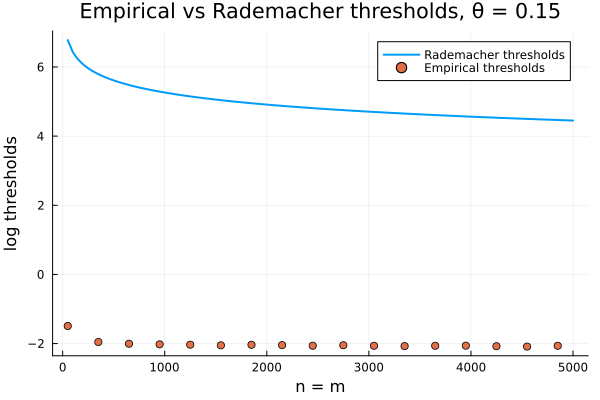
\includegraphics[width = \linewidth]{chapters/two-sample-testing/figures/ch4/emp_radem_plot_fixed_theta.png}
    \end{subfigure}
    \begin{subfigure}{0.32\textwidth}
        \centering
        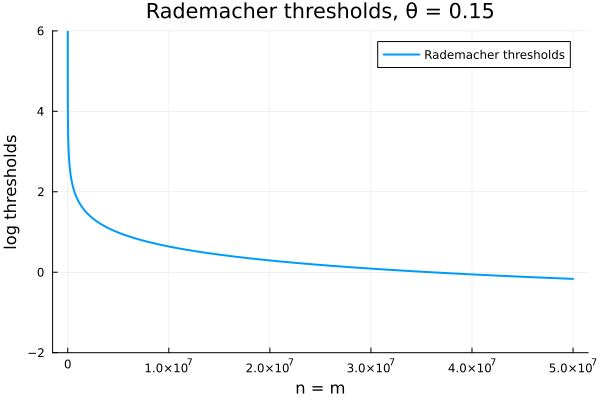
\includegraphics[width = \linewidth]{chapters/two-sample-testing/figures/ch4/radem_plot_vary_theta.png}
    \end{subfigure}
    \caption{}
    \label{fig:radem_threshold_plots}
\end{figure}

% polished end



% This section develops a uniform, nonparametric threshold for hypothesis testing derived from Rademacher complexity. The primary objective is to establish a concentration inequality for the distance between two hierarchical estimators. Intuitively, given two laws of random probability measure $Q_1, Q_2,$ whether the distance function $d$ is WoW or HIPM, $d\left(Q^1_{n,m}, Q^2_{n,m} \right)$ should be close to $d\left(Q^1, Q^2\right).$ Concentration inequality quantifies how close it will be for a given probability level. In particular, for $\theta \in (0,1)$, it gives us the radius $r(n, m, \theta)$ depending on $n, m$ and $\theta$ such that probability that $d\left(Q^1_{n,m}, Q^2_{n,m} \right)$ is within $r(n, m, \theta)$ radius from $d\left(Q^1, Q^2\right)$ is higher than $1 - \theta.$ This implies that under the null hypothesis, for every $\theta \in (0, 1),$ we know that $d\left(Q^1_{n,m}, Q^2_{n,m} \right)$ will be smaller than radius $r(n, m, \theta)$ with probability at least $1 - \theta.$ So, if we use $r(n, m, \theta)$ as a threshold function, and reject $H_0$ whenever 
% \[
% d\left(Q^1_{n,m}, Q^2_{n,m} \right) > r(n, m, \theta),
% \]
% we are guaranteed that the probability of making a Type I error is at most $\theta.$ Let us now discuss how to obtain the threshold function $r(n, m, \theta)$ and how it is related to the Rademacher complexity of the function class which defines the distance function.

% The main tool for obtaining such a result is Talagrand’s inequality (see Proposition B.1 in \cite{sriperumbudur2012empirical}). The radius function, as described above, is provided for a random variable that has a specific form, which also includes integral probability metrics. The dominant term in the radius function is the expected value of the random variable of interest. Following standard symmetrization arguments from empirical process theory, we bound this expectation using the Rademacher complexity of the underlying function class. This approach yields the following theoretical results:








% Recall that our focus is on the nonparametric setting, meaning that we do not make any assumptions on the laws of random probability measures. Given two such laws, $Q^1, Q^2 \in \probprobx$, we observe hierarchical samples from which we compute the distance between hierarchical estimators, $d(Q^1_{n,m}, Q^2_{n,m})$. In this section, we study testing schemes based on two distance functions: the Wasserstein-over-Wasserstein distance and the Hierarchical IPM. Recall that both of these distances are special cases of Integral Probability Metric.  

% The main idea of our testing scheme is to construct a rejection region such that the probability of observing a random variable falling into this region under the null hypothesis is small. Typically, this is achieved by comparing $d(Q^1_{n,m}, Q^2_{n,m})$ to its quantile under $H_0$. In our setting, however, the quantile is unknown. Instead, for a fixed probability level $\theta$ and sample sizes $n$ and $m$, we obtain a threshold $f(n, m, \theta)$ such that the probability of observing $d(Q^1_{n,m}, Q^2_{n,m})$ exceeding this threshold is at most $\theta$. Therefore, the corresponding rejection region takes the form $(f(n,m, \theta), \infty).$



% Although Talagrand’s theorem is quite general, in that it allows random variables taking values in abstract spaces beyond $\R^d$, we still face the challenge that we do not observe i.i.d. samples from $Q^1$ and $Q^2$. To overcome this issue, we decompose the gap
% \begin{align*}
% \left| \dlip(Q_{n,m}^1,Q_{n,m}^2) - \dlip(Q^1,Q^2) \right| 
% &\leq \left| \dlip(Q_{n,m}^1,Q_{n,m}^2) - \dlip(Q_n^1,Q_n^2) \right| \\
% &\quad + \left| \dlip(Q_n^1,Q_n^2) - \dlip(Q^1,Q^2) \right|,
% \end{align*}
% where $Q^1_n = \frac{1}{n}\sum_{i = 1}^n\delta_{\widetilde{P}^1_i}$, $Q^2_n = \frac{1}{n}\sum_{i = 1}^n\delta_{\widetilde{P}^2_i}$, and $\widetilde{P}^1_1,\ldots,\widetilde{P}^1_n\overset{\mathrm{i.i.d.}}{\sim}Q^1, \widetilde{P}^2_1,\ldots,\widetilde{P}^2_n\overset{\mathrm{i.i.d.}}{\sim}Q^2.$ 
% \par The first term in the upper bound quantifies the difference between the empirical distance derived from exchangeable sequences of random variables and the distance that would be obtained from i.i.d. samples drawn from the laws of RPMs. The second term measures the discrepancy between the empirical distance obtained from i.i.d. samples from the laws of random measures and the true distance. We decompose the gap in this way because each of the deviations can be controlled in probability. Bounding the second term in probability is studied in \cite{sriperumbudur2012empirical} for the general IPM, and the corresponding threshold depends on the Rademacher complexity of the function class over which the IPM is defined.
% in the theorem below if we just say bounded, we need the closed set. Otherwise it is not polish.
% \begin{theorem}[Threshold for HIPM] \label{theorem::radem_threshold_hipm}
% Let $\X$ be a compact subset of  $\R^d$, and $Q^1,Q^2 \in \probprobx.$ Then, there exists a function $r_d(n, m, \theta)$ such that for all $n, m \geq 1$ and $\theta \in (0,1)$
% \[
% \mathbb{P}\Big( \big|\dlip Q^1_{n,m}, Q^2_{n,m}) - \dlip Q^1, Q^2) \big| \geq r_d(n,m,\theta)\Big) \leq \theta,
% \]
% where for fixed $\theta$,
% \[
% r_d(n, m, \theta) = 
% \begin{cases}
%     O \left( \frac{1}{\sqrt{n}} + \frac{1}{\sqrt{m}}\right) ,\ & \text{if } d= 1 \\
%     O \left( \frac{1}{\sqrt{n}}\log(n) + \frac{1}{\sqrt{m}}\log(m)\right) ,\ & \text{if } d = 2 \\
%     O \left( \frac{1}{n^{\frac{1}{d}}} + \frac{1}{m^{\frac{1}{d}}}\right) ,\ & \text{if } d > 2
% \end{cases}
% \]







% \label{theorem::radem_threshold_hipm}
% Given $\X = [a,b]$, let $ K = b-a,$ and $Q^1,Q^2 \in \probprobx$. Then, $\forall \theta \in (0,1)$ 
% $$
% \mathbb{P}\left( \left| \dlip(Q_{n,m}^1, Q_{n,m}^2) - \dlip(Q^1, Q^2) \right| \geq 2 \left( 2c_2\left(n, m, \frac{\theta}{2}\right) + c_1\left(n, \frac{\theta}{2}\right) \right) \right) \leq \theta,
% $$
% where 
% \begin{align*}
%     &c_1(n, \theta) = \frac{1280K\sqrt{\log(2)}}{\sqrt{n}} + \sqrt{\frac{4K^2\log\left(\frac{1}{\theta}\right)}{n}} + \frac{4K}{3n}\log\left(\frac{1}{\theta}\right) + \frac{32\sqrt{10K^2\log\left(\frac{1}{\theta}\right)\sqrt{\log(2)}}}{n^{3/4}}, \\
%     &c_2(n,m, \theta) = \frac{256K \sqrt{\log (2)}}{\sqrt{m}} + \sqrt{\frac{K^2 \log (\frac{1}{\theta})}{2n}}.
% \end{align*}
% A similar theorem is obtained for the Wasserstein over Wasserstein distance. 
% \begin{theorem}[Threshold for WoW]
% \label{theorem::radem_threshold_wow}
% Let $\X$ be a compact subset of  $\R^d$, and $Q^1,Q^2 \in \probprobx.$ Then, there exists an integer $N \geq 1$ and a function $r_d(n, m, \theta)$ such that for all $n \geq N, m \geq 1$ and $\theta \in (0, 1)$
% \[
% \mathbb{P}\left( \left| \WW(Q^1_{n,m}, Q^2_{n,m}) - \WW(Q^1, Q^2)\right| \geq r_d(n, m, \theta) \right) \leq \theta,
% \]
% where for fixed $\theta$
% \[
% r_d(n, m, \theta) = 
% \begin{cases}
%     O \left(\frac{\log(\log(n))}{\log(n)} +  \frac{1}{\sqrt{n}} + \frac{1}{\sqrt{m}}\right) ,\ & \text{if } d= 1 \\
%     O \left(\frac{\log(\log(n))}{\log(n)} + \frac{1}{\sqrt{n}}\log(n) + \frac{1}{\sqrt{m}}\log(m)\right) ,\ & \text{if } d = 2 \\
%     O \left(\frac{\log(\log(n))}{\log(n)} + \frac{1}{n^{\frac{1}{d}}} + \frac{1}{m^{\frac{1}{d}}}\right) ,\ & \text{if } d > 2
% \end{cases}
% \]

% \end{theorem}
% \begin{theorem}[Threshold for WoW]
% \label{theorem::radem_threshold_hipm}
% Given $\X = [a,b]$, Let $ K = b-a,$ and $Q^1,Q^2 \in \probprobx$. Then, there exist constants $C,N$ such that for all $n \geq N$ and for all $\theta \in (0,1)$ 
% $$
% \mathbb{P}\left( \left| \WW(Q_{n,m}^1, Q_{n,m}^2) - \WW(Q^1, Q^2) \right| \geq 2 \left( 2c_2\left(n, m, \frac{\theta}{2}\right) + c_1\left(n, \frac{\theta}{2}\right) \right) \right) \leq \theta,
% $$
% where 
% \begin{align*}
%     &c_1(n, \theta) = C \frac{\log (\log(n))}{\log (n)} + \sqrt{\frac{4K^2 \log \left( \frac{1}{\theta}\right)}{n}} + \frac{4K\log  \left( \frac{1}{\theta}\right)}{3n} + 2 \sqrt{\frac{2K\log \left(\frac{1}{\theta} \right)}{n}C \frac{\log (\log(n))}{\log (n)}}, \\
%     &c_2(n,m, \theta) = \frac{256K \sqrt{\log (2)}}{\sqrt{m}} + \sqrt{\frac{K^2 \log (\frac{1}{\theta})}{2n}}.
% \end{align*}
% \end{theorem}
% \begin{remark}
% If $\X = [a,b]$, then the exact form of the threshold function in Theorem \ref{theorem::radem_threshold_hipm} can be obtained as the bound for the Rademacher complexity is known in exact form. Then we have a finite sample guarantee for the Type I error. Note that in the case of WoW, even if the exact threshold was known, we would have a finite sample guarantee only after some integer $N \geq 1.$ 
% \end{remark}
% \begin{remark}
%     Theorems \ref{theorem::radem_threshold_hipm} and \ref{theorem::radem_threshold_wow} can be extended to more general spaces $\X$ as long as one can bound the Rademacher complexity of the function class over which the IPM is defined. Whether an exact threshold can be obtained depends on whether the bound on the Rademacher complexity is exact or not.
% \end{remark}
% Note that in the theorem for WoW, a finite-sample guarantee is obtained only after some integer $N$, and the threshold is known up to a constant.

% Let us start with HIPM. For fixed $\theta,$ the function $c_1(n, \theta)$ decays to $0$ at the rate $O\!\left(\frac{1}{\sqrt{n}}\right).$ The function $c_2(n,m, \theta)$ converges to $0$ at the rate $O\!\left(\frac{1}{\sqrt{m}} + \frac{1}{\sqrt{n}}\right).$ Therefore, the threshold function for HIPM decays to $0$ at the rate $O\left(\frac{1}{\sqrt{m}} + \frac{1}{\sqrt{n}}\right).$

% On the other hand, for WoW, the function $c_1(n,\theta)$ has convergence rate $O\left(\frac{\log (\log (n))}{\log(n)}\right).$ Note that $c_2(n, m, \theta)$ is the same as in HIPM, since the bound we use is exactly the same as for HIPM (see proof in \ref{appendix:rademacher}). Therefore, the threshold function for WoW decays to $0$ at the rate  $O\left(\frac{1}{\sqrt{n}} + \frac{1}{\sqrt{m}} + \frac{\log( \log(n))}{\log(n)}\right).$

% Let us also note why we have two different functions $c_1$ and $c_2.$ Recall that we decompose the gap 
% \begin{align*}
% \left| \dlip(Q_{n,m}^1,Q_{n,m}^2) - \dlip(Q^1,Q^2) \right| 
% &\leq \left| \dlip(Q_{n,m}^1,Q_{n,m}^2) - \dlip(Q_n^1,Q_n^2) \right| \\
% &\quad + \left| \dlip(Q_n^1,Q_n^2) - \dlip(Q^1,Q^2) \right|.
% \end{align*}
% The function $c_1(n, \theta)$ corresponds to the bound for the gap $\left|d(Q^1_n, Q^2_n) - d(Q^1, Q^2)\right|.$ The bound for this gap includes the Rademacher complexity of the function class over which the Integral Probability Metric is defined, along with some terms arising from Talagrand's inequality. These additional terms have the convergence rate $O\left(\frac{1}{\sqrt{n}}\right).$ Since the Rademacher complexity of the function class for HIPM also has the rate $O\left(\frac{1}{\sqrt{n}}\right)$ and therefore does not worsen the rate coming from Talagrand's inequality, using HIPM is favorable over WoW. The function $c_2(n, m, \theta)$ corresponds to the bound for the gap $\left|d(Q^1_{n,m}, Q^2_{n,m}) - d(Q^1_n, Q^2_n)\right|.$ The bound we use for this gap is the same for both HIPM and WoW, and that is why the threshold function for this term is the same in both cases.


% The consequence of the theorems above is the testing scheme which, given some significance level $\theta,$ rejects the null hypothesis whenever the observed distance between hierarchical estimators exceeds the threshold from the above theorems. In addition to controlling the Type I error, these theorems also ensure consistency. Intuitively, under $H_1,$ the observed distance $d(Q^1_{n,m}, Q^2_{n,m}),$ whether $d$ is WoW or HIPM, will be close to $d(Q^1,Q^2).$ Hence, as long as the threshold $f(n, m, \theta)$ converges to $0$ as $n,m \to \infty,$ we will eventually have $d(Q^1_{n,m}, Q^2_{n,m}) > f(n, m, \theta).$ The theorem below formalizes this intuition. Note that in the limits below, there is no dependency between $n$ and $m$ in how they converge to infinity.
% \begin{theorem}[Consistency for HIPM]
% \label{theorem::radem_consistency_hipm}
% Let $\X$ be a compact subset of  $\R^d$, and $Q^1,Q^2 \in \probprobx.$ Let also $\theta$ denote the significance level, and let $r_d(n, m, \theta)$ be the threshold function from Theorem \ref{theorem::radem_threshold_hipm}. Then:
% \begin{itemize}
%     \item Type I error: if $Q^1 = Q^2$, then  
%     $$\mathbb{P}\left( \dlip(Q_{n,m}^1, Q_{n,m}^2) > r_d(n,m, \theta) \right) \leq \theta \quad \text{for all } n, m \geq 1.$$
%     \item Consistency: if $Q^1 \neq Q^2$ then,  
%     $$\lim_{n,m\to \infty}\mathbb{P}\left( \dlip(Q_{n,m}^1, Q_{n,m}^2) > r_d(n,m, \theta) \right) = 1.$$
% \end{itemize}
% \end{theorem}
% \begin{theorem}[Consistency for WoW]
% \label{theorem::radem_consistency_wow}
% Let $\X$ be a compact subset of  $\R^d$, and $Q^1,Q^2 \in \probprobx.$ Let also $\theta$ denote the significance level, and let $r_d(n, m, \theta)$ be the threshold function from Theorem \ref{theorem::radem_threshold_wow}. Then, there exists $N\geq 1$ such that
% \begin{itemize}
%     \item Type I error: if $Q^1 = Q^2$, then  
%     $$\mathbb{P}\left( \WW(Q_{n,m}^1, Q_{n,m}^2) > r_d(n,m, \theta) \right) \leq \theta \quad \text{for all } n\geq N, m \geq 1.$$
%     \item Consistency: if $Q^1 \neq Q^2$ then,  
%     $$\lim_{n,m\to \infty}\mathbb{P}\left( \WW(Q_{n,m}^1, Q_{n,m}^2) > r_d(n,m, \theta) \right) = 1.$$
% \end{itemize}
% \end{theorem}
% While theoretically appealing, the aforementioned theorems have practical limitations. Achieving high power requires the threshold to decay to zero at a sufficiently fast rate. However, the logarithmic terms present in the threshold using WoW distance result in a threshold function that converges to zero at a suboptimal rate. Although using the HIPM, we obtain a parametric rate, the constant term within the function makes the testing scheme impractical.

% These limitations are demonstrated by our numerical simulations. We restrict our simulations to the HIPM as the threshold associated WoW is even more conservative than that of the HIPM. 

% Suppose that we have two different laws of RPM, $Q^1, Q^2 \in \probprobx.$ For fixed probability level $\theta\in(0,1)$, to obtain the low type II error, that is, the probability of not rejecting null hypothesis when it is false, it is desired to have the theoretical threshold less than the empirical threshold, which is defined as the $(1-\theta)$-quantile of the random variable $\dlip(Q_{n,m}^1, Q_{n,m}^2)$. In the figure below, we display how theoretical and empirical thresholds differ for fixed $\theta$ when we increase $n $ and $m.$

% Fix $\theta = 0.15$ and consider the two Dirichlet processes $Q^1 = \text{DP}(1.0, P_0)$, $Q^2 = \text{DP}(1.5, P_0)$, where $P_1 = \law \left(Z \right)$,
% \[
% Z = \begin{cases}
% 0.25X - 1, & \text{with probability } 0.5, \\[6pt]
% 0.25X + 0.75, & \text{with probability } 0.5.
% \end{cases}
% \]
% $X \sim \text{Unif}(0,1).$

% As we see in Figure \ref{fig:radem_threshold_plots}, the theoretical threshold is very large compared to the empirical threshold even when $n$ and $m$ are big. The consequence of this is that the null hypothesis is never rejected when it is false. The reason behind the very large theoretical threshold is that it is uniform over all laws of random probability measures.

% \begin{figure}[H]
%     \centering
%     \begin{subfigure}{0.32\textwidth}
%         \centering
%         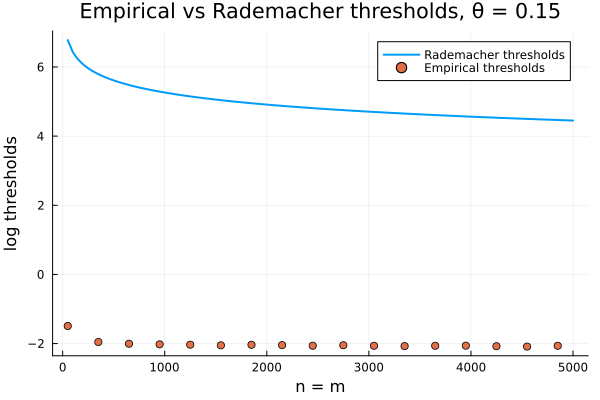
\includegraphics[width = \linewidth]{chapters/two-sample-testing/figures/ch4/emp_radem_plot_fixed_theta.png}
%     \end{subfigure}
%     \begin{subfigure}{0.32\textwidth}
%         \centering
%         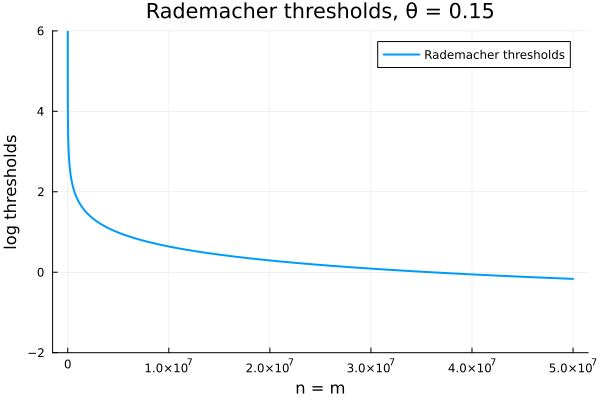
\includegraphics[width = \linewidth]{chapters/two-sample-testing/figures/ch4/radem_plot_vary_theta.png}
%     \end{subfigure}
%     \caption{}
%     \label{fig:radem_threshold_plots}
% \end{figure}

% summary: uniform, nonparametric thresholds via Rademacher complexity, HIPM yields faster rates than WoW,thresholds are overly conservative in practice.




\section{Practical thresholds via a permutation approach}\label{section::permutation}

% Recall that the threshold via Rademacher complexity overestimates the quantile function of the observed distance for each $\theta \in (0,1)$ under the null hypothesis. Even though, for a fixed probability level $\theta,$ we can obtain a rejection region with probability $1 - \theta,$ as long as $n$ and $m$ are sufficiently large, that region is much smaller than the region corresponding to the true quantile. The remedy for this is to use the permutation approach. 

In this section, we introduce a permutation-based framework for two-sample testing that yields improved performance in practice. As discussed earlier, the threshold derived from Rademacher complexity is overly conservative, resulting in low power for finite sample sizes. The permutation approach alleviates this issue by providing a more accurate approximation of the quantile function of the test statistic under the null hypothesis $H_0,$ while typically yielding a much smaller threshold under the alternative.
% In this section, we introduce a more practical approach for two-sample testing via the permutation approach. Recall, that the main problem of the threshold obtained via Rademacher complexity was that it was very large for practical applications. Threshold via permutation approach remedies that problem. In particular, it provides a better approximation for the quantile function of the observed random variable under $H_0$, and whenever null hypothesis is false, it does not require as large an amount of data to make a rejection. The intuition behind this is that the threshold via permutation depends on the laws of random probabilities that generated the data, whereas the threshold via Rademacher complexity works uniformly over all laws of RPM's. Let us now introduce the permutation approach.
% This is done by first obtaining approximate samples of the observed distance and then computing the empirical quantile. The practical advantage of this approach is that, since the quantile is estimated from approximate samples of the test statistic, the rejection region is larger than that obtained via the threshold based on Rademacher complexity. This is intuitive, since the latter works uniformly over all laws of random probability measures, while the former is derived from the data-generating laws $Q^1$ and $Q^2.$ 
Recall that, given $Q^1,Q^2\in \probprobx$, we observe
\[
\widehat{P}^1_{1,m},\cdots, \widehat{P}^1_{n,m} \overset{\iid}{\sim} Q^{1,(m)}, \quad 
\widehat{P}^2_{1,m},\cdots, \widehat{P}^2_{n,m} \overset{\iid}{\sim} Q^{2,(m)}.
\]
Using these samples, we compute the distance $d(\widehat{Q}^1_{n,m}, \widehat{Q}^2_{n,m})$, where $d$ can be either WoW or HIPM. Our goal is to estimate the quantile function of the random variable $d(\widehat{Q}^1_{n,m}, \widehat{Q}^2_{n,m})$ assuming that $Q^1 = Q^2,$ and use it as a testing threshold. Ideally, such a quantile could be estimated empirically from multiple independent realizations of this random variable. In practice, however, only a single realization is available.

We circumvent this limitation by noting that under the null hypothesis $Q^1 = Q^2$, all random probability measures $\widehat{P}^k_{i,m}$ share the same distribution. Consequently, if we randomly shuffle these objects and recompute the distance, the resulting value constitutes another realization from the distribution of $d(\widehat{Q}^1_{n,m}, \widehat{Q}^2_{n,m})$. By repeating this process, we can obtain several samples of the distance between hierarchical estimators. Although these samples are not independent, this dependence is typically negligible in practice when the sample sizes $n$ and $m$ are sufficiently large.

We now formalize this procedure. Recall the hierarchical estimators 
\[
\widehat{Q}^1_{n,m} = \frac{1}{n} \sum_{i = 1}^n \delta_{\widehat{P}^1_{i,m}} \quad \text{and} \quad \widehat{Q}^2_{n,m} = \frac{1}{n} \sum_{i = 1}^n \delta_{\widehat{P}^2_{i,m}}.
\]
To implement the permutation test, we first form the pooled collection of random probability measures
\[
\left\{ \widehat{P}_{1,m},\cdots, \widehat{P}_{2n,m}  \right\} :=\left\{ \widehat{P}^1_{1,m}, \dots, \widehat{P}^1_{n,m}, \widehat{P}^2_{1,m}, \dots, \widehat{P}^2_{n,m} \right\} .
\]
A random permutation of this collection is induced by a vector $R = (R_1, \dots, R_{2n})$ sampled uniformly from the set of all permutations of $\{1, \dots, 2n\}$. For notational brevity, we omit the explicit dependence of $R$ on $n$ and $m$.

We then define the permuted hierarchical estimators as
\[
\widetilde{Q}^1_{n,m} = \frac{1}{n} \sum_{i = 1}^n \delta_{\widehat{P}_{R_i,m}} \quad \text{and} \quad \widetilde{Q}^2_{n,m} = \frac{1}{n} \sum_{i = n+1}^{2n} \delta_{\widehat{P}_{R_i,m}}.
\]
Finally, we compute the distance $d(\widetilde{Q}^1_{n,m}, \widetilde{Q}^2_{n,m}).$

Repeating this process, randomly permuting the pooled sample and recomputing the distance, yields the approximate samples of the distance between the hierarchical estimators of $Q^1$ and $Q^2$. Then, for a given significance level $\theta \in (0,1),$ we set the testing threshold equal to the empirical $(1-\theta)$-quantile of these values.

In practice, since we work with the hierarchical samples $\mathbf{X}_{n,m}, \mathbf{Y}_{n,m}$ permutation is implemented by exchanging the rows between or across them. The resulting procedure is summarized in Algorithm~\ref{algorithm::permutation_approach}.

\begin{center}
\begin{minipage}{0.85\textwidth} % Adjust 0.85 to make it narrower or wider
\begin{algorithm}[H]
\caption{Permutation test with $d \in \{\dlip,\WW\}$}
\label{algorithm::permutation_approach}
\begin{algorithmic}[1]
\Require Hierarchical samples $\mathbf{X}_{n,m},\mathbf{Y}_{n,m}$; significance level $\theta \in (0,1)$; number of permutations $n_\text{perm}$
\Ensure Decision: $1$ = reject $H_0$, $0$ = do not reject $H_0$

\State $T_{\mathrm{obs}} \gets d(\mathbf{X}_{n,m},\mathbf{Y}_{n,m})$ \Comment{Observed test statistic}
\State $\mathcal{Z} \gets \text{vcat}(\mathbf{X}_{n,m},\mathbf{Y}_{n,m})$ \Comment{Pool the $2n$ rows}
\For{$i=1,\ldots,n_\text{perm}$}
    \State $R \gets \text{permute}(\{1,\ldots,2n\})$
    \State $T_i \gets d(\mathcal{Z}_{R_{1:n}}, \mathcal{Z}_{R_{n+1:2n}})$ 
\EndFor

\State $r_\theta \gets \widehat{q}_{1-\theta}(T_1,\ldots,T_{n_\text{perm}})$ \Comment{Empirical $(1-\theta)$-quantile}
\State \Return $\mathbf{1}\{T_{\mathrm{obs}} > r_\theta\}$
\end{algorithmic}
\end{algorithm}
\end{minipage}
\end{center}

The theoretical properties of the proposed procedure are studied by analyzing the asymptotic distributions of the observed test statistic and the corresponding threshold under the null and alternative hypotheses. To this end, we appropriately rescale the observed distance and define the test statistic
\[
T_{n,m} = \sqrt{\frac{n}{2}}\dlip\left( \widehat{Q}^1_{n,m}, \widehat{Q}^2_{n,m} \right).
\]
The corresponding threshold is defined as
\[
r(n,m,\theta) = \inf \left\{ t \in \R : \mathbb{P}\left(\widetilde{T}_{n,m} > t \right) \leq \theta \right\},
\]
where 
\[
\widetilde{T}_{n,m} = \sqrt{\frac{n}{2}} \, d(\widetilde{Q}^1_{n,m}, \widetilde{Q}^2_{n,m}).
\]
Note that this scaling is introduced solely for theoretical analysis and is not required for the practical implementation of the algorithm.

In this section, we restrict attention to the case $d=\dlip$. Deriving the asymptotic distribution of $T_{n,m}$ depends on whether the function class over which the corresponding integral probability metric is defined is a Donsker class (see the proof of Theorem~\ref{theorem::asympt_distr_dlip}). At present, we are unable to verify this property for the WoW distance, and therefore do not establish the theoretical guarantees.

To conclude, we establish asymptotic level-$\theta$ control and consistency guarantees for the proposed testing scheme.
\begin{theorem}[Consistency of permutation approach]
\label{theorem::perm__consistency_dlip}
Given $\X = [a,b]$, and $Q^1, Q^2 \in \probprobx$. Let $\theta$ denote the significance level and $r(n,m, \theta)$ be a threshold from permutation approach. Then
\begin{itemize}
    \item if $Q^1 = Q^2,$ then $$ \limsup_{n,m\to \infty} \mathbb{P}\left(T_{n,m}>r(n,m, \theta)\right)\leq \theta.$$
    \item if $Q^1 \neq Q^2,$ then $$ \lim_{n,m\to \infty} \mathbb{P}\left(T_{n,m} > r(n,m,\theta) \right) = 1.$$
\end{itemize}
\end{theorem}
% Let us see how the threshold via the permutation approach works in practice. We are interested in the type I error, (false positive rate, FPR), and true positive rate (TPR) of the testing scheme, meaning:
% \begin{itemize}
%     \item Given two hierarchical samples from the same laws of RPM, how often does the testing scheme reject the null hypothesis?
%     \item Given two hierarchical samples from two different laws of RPM, how often does the testing scheme reject the null hypothesis?
% \end{itemize}
% In addition to Type I error and TPR, we look at the trade-off between them, i.e., we plot the ROC curve that shows the behaviour of TPR as a function of the FPR.
% In the first figure we are working with the random probability measure defined as
% \begin{align*}
% &\widetilde{P}^1  = \text{TN}(\mu_1, 1) \quad \text{where }\mu_1\sim \mathcal{N}(1.0, 1)\\
% &\widetilde{P}^2  = \text{TN}(\mu_2, 1) \quad \text{where }\mu_2\sim \mathcal{N}(1.5, 1),
% \end{align*}
% where TN denotes the truncated normal distribution on [0,1]. We set the number of permutations equal to $80.$ To get the false positive and true positive rates, we simulate hierarchical measures from the pairs $\left(\mathcal{L}\left(\widetilde{P}^1 \right),\mathcal{L}\left(\widetilde{P}^1 \right) \right)$ and $\left(\mathcal{L}\left(\widetilde{P}^1 \right),\mathcal{L}\left(\widetilde{P}^2 \right) \right).$ We study the two cases: On the first row of Figure~\ref{fig:normal_normal}, $n = 35, m = 10$, and on the second row $n = 70, m = 15.$

% \begin{figure}[h!]
%     \centering
%     \begin{subfigure}{0.32\textwidth}
%         \centering
%         
\includegraphics[width = \linewidth]{figures/ch5/normal_normal/falsepositive_rates_normal_normal_mu_1=1.0_n=35_m=10_s=150_permutations=80_samemeasures.png}
%     \end{subfigure}
%     \begin{subfigure}{0.32\textwidth}
%         \centering
%         
\includegraphics[width = \linewidth]{figures/ch5/normal_normal/truepositive_rates_normal_normal_mu_1=1.0_mu_2=1.5_n=35_m=10_s=150_permutations=80_diffmeasures.png}
%     \end{subfigure}
%     \begin{subfigure}{0.32\textwidth}
%         \centering
%         
\includegraphics[width = \linewidth]{figures/ch5/normal_normal/ROC_normal_normal_mu_1=1.0_mu_2=1.5_n=35_m=10_s=150_permutations=80.png}
%     \end{subfigure}

%     \begin{subfigure}{0.32\textwidth}
%         \centering
%         
\includegraphics[width = \linewidth]{figures/ch5/normal_normal/falsepositive_rates_normal_normal_mu_1=1.0_n=70_m=15_s=150_permutations=80_samemeasures.png}
%     \end{subfigure}
%     \begin{subfigure}{0.32\textwidth}
%         \centering
%         
\includegraphics[width = \linewidth]{figures/ch5/normal_normal/truepositive_rates_normal_normal_mu_1=1.0_mu_2=1.5_n=70_m=15_s=150_permutations=80_diffmeasures.png}
%     \end{subfigure}
%     \begin{subfigure}{0.32\textwidth}
%         \centering
%         
\includegraphics[width = \linewidth]{figures/ch5/normal_normal/ROC_normal_normal_mu_1=1.0_mu_2=1.5_n=70_m=15_s=150_permutations=80.png}
%     \end{subfigure}
%     \caption{}
%     \label{fig:normal_normal}
% \end{figure}

% As we see from the plot, for both of the distance functions, the Type I error is well controlled. Also, type II error is becoming low as we increase $n$ and $m$. In addition, the ROC curve is much better for both distance functions than the random guessing.

% What is not expected from the simulations is that we also control Type I error for the Wasserstein over Wasserstein. In theory, we could not show that under the null hypothesis, the test statistic has the same convergence properties as that with HIPM; however, in practice, it performs well. 

% In Figure~\ref {fig:DP_DP}, we are working with the same Dirichlet processes as the ones we used for Figure~\ref{fig:radem_threshold_plots}.

% Here, on the first row $n = 70, m = 7$, and on the second row $n = 120, m = 70.$ 

% \begin{figure}[H]
%     \centering
%     \begin{subfigure}{0.32\textwidth}
%         \centering
%         
\includegraphics[width = \linewidth]{figures/ch5/dirichlet/falsepositive_rates_dirichlet_diffalpha_n=70_m=7_s=150_permutations=80_samemeasures.png}
%     \end{subfigure}
%     \begin{subfigure}{0.32\textwidth}
%         \centering
%         
\includegraphics[width = \linewidth]{figures/ch5/dirichlet/truepositive_rates_dirichlet_diffalpha_n=70_m=7_s=150_permutations=80_diffmeasures.png}
%     \end{subfigure}
%     \begin{subfigure}{0.32\textwidth}
%         \centering
%         
\includegraphics[width = \linewidth]{figures/ch5/dirichlet/ROC_dirichlet_diffalpha_alpha_1=1.0_alpha_2=1.5_n=70_m=7_s=150_permutations=80.png}
%     \end{subfigure}

%     \begin{subfigure}{0.32\textwidth}
%         \centering
%         
\includegraphics[width = \linewidth]{figures/ch5/dirichlet/falsepositive_rates_dirichlet_diffalpha_n=120_m=70_s=150_permutations=80_samemeasures.png}
%     \end{subfigure}
%     \begin{subfigure}{0.32\textwidth}
%         \centering
%         
\includegraphics[width = \linewidth]{figures/ch5/dirichlet/truepositive_rates_dirichlet_diffalpha_n=120_m=70_s=150_permutations=80_diffmeasures.png}
%     \end{subfigure}
%     \begin{subfigure}{0.32\textwidth}
%         \centering
%         
\includegraphics[width = \linewidth]{figures/ch5/dirichlet/ROC_dirichlet_diffalpha_alpha_1=1.0_alpha_2=1.5_n=120_m=70_s=150_permutations=80.png}
%     \end{subfigure}
%     \caption{}
%     \label{fig:DP_DP}
% \end{figure}


% As we see from the plot, for both of the distance functions, the Type I error is well controlled. Also, type II error is becoming low as we increase $n$ and $m$. In addition, the ROC curve is much better for both distance functions than the random guessing.

% What is not expected from the simulations is that we also control Type I error for the Wasserstein over Wasserstein. In theory, we could not show that under the null hypothesis, the test statistic has the same convergence properties as that with HIPM; however, in practice, it performs well. 

% In Figure~\ref {fig:DP_DP}, we are working with the same Dirichlet processes as the ones we used for Figure~\ref{fig:radem_threshold_plots}.
% Similarly to the Figure~\ref{fig:normal_normal}, in Figure~\ref{fig:DP_DP}, we also see that the Type I error is well controlled. Here, the true positive rate is improving slowly as we increase $n$ and $m$ but this is because the $\alpha$'s we chose for random probability measures are very close to each other. 







% For a given probability level $\theta,$ if the frequency of those samples exceeding the observed distance is smaller than $\theta,$ this means that the observed distance is larger than the empirical $(1-\theta)$-quantile from those samples. Even though in practice we consider a finite number of permutations, to study the theoretical properties of this approach we define the permutation threshold at probability level $\theta$ as the $(1 - \theta)$-quantile of the random variable 
% $$ 
% \widetilde{T}_{n,m} = \sqrt{\frac{n}{2}} \, d(\widetilde{Q}^1_{n,m}, \widetilde{Q}^2_{n,m}), 
% $$
% where the only source of randomness is the permutation, and $\{ \widehat{P}^1_{1,m},\ldots,\widehat{P}^1_{n,m},\widehat{P}^2_{1,m},...\widehat{P}^2_{n,m} \}$ are fixed. Note that here we have the factor $\sqrt{\frac{n}{2}}.$ Note that in this case, the test statistic is 
% \[
% T_{n,m} = \frac{n}{2}\dlip\left( \widehat{Q}^1_{n,m}, \widehat{Q}^2_{n,m} \right).
% \]
% Comparing empirical quantile from permuted samples to the observed distance $d(\widehat{Q}^1_{n,m}, Q^2_{n,m
% })$ is equivalent to comparing their associated scaled versions to each other. This scaling factor is needed to study the asymptotic distribution of random variables $T_{n,m}$ and $\widetilde{T}_{n,m}.$

% The testing scheme has the following structure: after observing hierarchical samples $\mathbf{X}\sim Q^1$ and $\mathbf{Y}\sim Q^2,$ we obtain the samples $\widetilde{T}^1_{n,m}, ..., \widetilde{T}^S_{n,m}$ from the permutation approach, and reject the null hypothesis if 
% \[
% T_{n,m} > \widehat{c}(n,m,\theta),
% \]
% where $\widehat{c}(n,m,\theta)$ is the empirical quantile of the random variable $\widehat{T}_{n,m}$ computed from the samples $\widetilde{T}^1_{n,m}, ..., \widetilde{T}^S_{n,m}.$ 

% Note that it is equivalent to reject $H_0$ if 
% $$
% \frac{1}{S}\sum_{i = 1}^S \mathbf{1}\!\left(T_{n,m} < \widetilde{T}^i_{n,m}\right) \leq \theta.
% $$
% To sum up, the algorithm has the following structure: 

% \begin{algorithm}
% \caption{Permutation Test: Reject/Do Not Reject $H_0$, $ d \in \{\dlip,\WW\}$ }
% \label{algorithm:permutation_approach}
% \begin{algorithmic}[1]
% \Require Hierarchical samples $X, \mathbf{Y}$; significance level $\theta$; number of permutations $n_{\mathrm{perm}}$
% \Ensure Decision: $1=$Reject $H_0$, $0=$Do not reject $H_0$

% \State $d_{\mathrm{obs}} \gets d(X, \mathbf{Y})$ \hfill \Comment{Compute observed distance}
% \State $Pooled\_sample \gets \mathrm{concat}(X, \mathbf{Y})$ \hfill \Comment{Pool both samples}
% \State $n \gets \text{number of rows in } X$
% \State $permuted\_distances \gets [\ ]$ \hfill \Comment{Initialize storage for permuted distances}

% \For{$b = 1$ to $n_{\mathrm{perm}}$}
%   \State $R \gets$ random permutation of $\{1, \dots, 2n\}$
%   \State $X' \gets Pooled\_sample[{R(1:n)}]$ \hfill \Comment{choose first $n$ random rows from pooled samples}
%   \State $\mathbf{Y}' \gets Pooled\_sample[{R(n+1:2n)}]$ \hfill \Comment{choose second $n$ random rows from pooled samples}
%   \State append $d(X', \mathbf{Y}')$ to $permuted\_distances$
% \EndFor

% \State $t_{\theta} \gets \operatorname{Quantile}(permuted\_distances,\,1 - \theta)$ \hfill \Comment{Compute threshold}
% \State \Return $\mathbbm{1}\{\,d_{\mathrm{obs}} > t_{\theta}\,\}$ \hfill \Comment{Reject if observed distance exceeds threshold}
% \end{algorithmic}
% \end{algorithm}
% To study the theoretical properties of this testing scheme, we consider the behaviour of 
% $$
% \mathbb{P}\!\left(T_{n,m} > c(n,m,\theta)\right)
% $$
% under the null and alternative hypotheses, where $c(n,m,\theta)$ is the theoretical quantile of $\widetilde{T}_{n,m},$ defined as
% $$
% c(n,m,\theta) = \inf \left\{ t \in \R : \mathbb{P}\left(\widetilde{T}_{n,m} > t \right) \leq \theta \right\}.
% $$
% We will call $c(n,m,\theta)$ the permutation threshold.

% The theoretical guarantees are obtained by studying the asymptotic distributions of $T_{n,m}$ and $c(n,m,\theta).$ 
\section{Simulation Studies}\label{section:simulations}
In this section, we examine the finite-sample performance of the proposed HIPM and WoW testing procedures. Our numerical analysis is organized into three parts. First, we investigate the validity of the permutation-based test by evaluating the Type I error rate and statistical power of both HIPM and WoW using a synthetic dataset. Second, we compare our methods with existing methods from the literature. Finally, we demonstrate the practical utility of the proposed framework through an application to a mortality dataset.

\subsection{Empirical Comparison Between HIPM and WoW}\label{subsection:hipm_wow_comparison}

We compare the use of HIPM and WoW within our permutation-based test by analysing the Type I error and the power in several simulated settings, considering both parametric and nonparametric data-generating processes, in settings that satisfy the assumptions of Theorem~\ref{theorem:perm_consistency_dlip} and in settings that do not, notably $\X = \R$, but are still of practical interest. We consider the following baselines for parametric and nonparametric models.
\begin{enumerate}
\item Parametric model that fulfills the assumptions:
\[
Q^1 = \mathcal{L}(\tilde P), \qquad \tilde P| \tilde \mu = \mathrm{Beta}( \tilde \mu, 1- \tilde \mu), \qquad \tilde \mu \sim \mathrm{Beta}(a_0 = 1, b_0 = 1);
\]
\item Parametric model that does not fulfill the assumptions:
\[
Q^1 = \mathcal{L}(\tilde P), \qquad \tilde P| \tilde \mu = \mathcal{N}(\tilde \mu, \sigma^2 = 1), \qquad \tilde \mu \sim \N(\mu_0 = 0, \sigma^2_0 = 1);
\]

\item Nonparametric model that fulfills the assumptions:
\[
Q^1 = \mathrm{DP}(\alpha = 1, P_0 = \mathrm{Unif}[0,1]);
\]
\item Nonparametric model that does not fulfill the assumptions:
\[
Q^1 = \mathrm{DP}(\alpha = 1, P_0 = N(0,1)),
\]
\end{enumerate}
where $\mathrm{Beta}(a,b)$ is the Beta distribution with shape parameters $a,b$, $\mathcal{N}(\mu, \sigma^2)$ is the Gaussian distribution with mean $\mu$ and variance $\sigma^2$, $\mathrm{Unif}[0,1]$ is the Uniform distribution on the interval $[0,1]$, and $\mathrm{DP}(\alpha, P_0)$ denotes the Dirichlet process with concentration $\alpha>0$ and base measure $P_0 \in \probx$. Note that if $P_0$ has full support on $\X$, $\mathrm{DP}(\alpha, P_0)$ has full weak support on $\probx$.

To investigate the behaviour of the Type I error, we simulate data $S = 1000$ times with $Q^1 = Q^2$ set equal to each of the four models above, perform our permutation-based test for both WoW and HIPM, and report the percentage of times it rejects the (correct) $H_0: Q^1 = Q^2$ for each significance level $\theta$. In each simulation, we set $n=m=n_{\text{perm}}= 100$.

The results are shown in Figure~\ref{figure:fp_wow_vs_hipm}, where we see that both WoW and HIPM control the Type I error at approximately the significance level $\theta$ across all simulation settings. We report only one of the four graphs, as the remaining graphs show no qualitative differences. Interestingly, WoW also appears to control the Type I error even though our theory does not guarantee it, and both methods behave well in unbounded settings.
\begin{figure}[H]
    \centering
      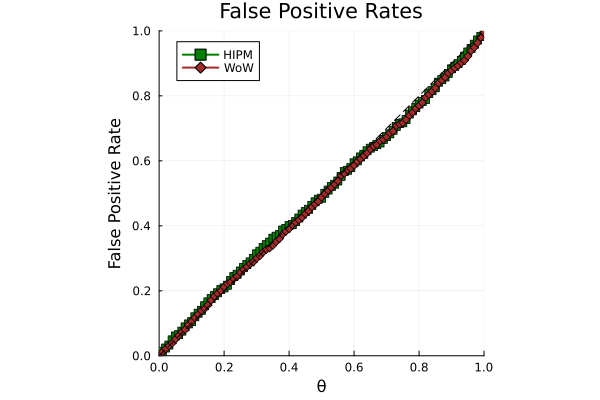
\includegraphics[width = 0.49\linewidth]{chapters/two-sample-testing/figures/wow_vs_hipm/fp_label=1_n=100_m=100_S=1000_n_perm=100.png}
    \caption{False Positive Rates for HIPM and WoW}
    \label{figure:fp_wow_vs_hipm}
\end{figure}
To investigate the power of the test, we simulate the data under the alternative hypothesis $Q^1 \neq Q^2$. For each of the four laws considered above, we associate an alternative law and estimate the power, resulting in the following four cases:
\begin{align*}
\text{A.} \quad & Q^1 = \mathcal{L}(\tilde P), \quad \tilde P| \tilde \mu = \mathrm{Beta}(\tilde \mu, 1-\tilde \mu), \quad \tilde \mu \sim \mathrm{Beta}(a_0 = 1, b_0 = 1) \\
                & Q^2 = \mathcal{L}(\tilde P), \quad \tilde P| \tilde \mu = \mathrm{Beta}(\tilde{\mu}, 1-\tilde{\mu}), \quad \tilde \mu \sim \mathrm{Beta}(a_0 = 1, b_0 = 1.5) \\[1em]
\text{B.} \quad & Q^1 = \mathcal{L}(\tilde P), \quad \tilde P| \tilde \mu = \N(\tilde \mu, \sigma^2 = 1), \quad \tilde \mu \sim \N(\mu_0 = 0, \sigma^2_0 = 1) \\
                & Q^2 = \mathcal{L}(\tilde P), \quad \tilde P| \tilde \mu = \N(\tilde \mu, \sigma^2 = 1), \quad \tilde \mu \sim \N(\mu_0 = 0, \sigma^2_0 = 1.5) \\[1em]
\text{C.} \quad & Q^1 = \mathrm{DP}(\alpha = 1, P_0 = \mathrm{Unif}[0,1]) \\
                & Q^2 = \mathrm{DP}(\alpha = 1, P_0 = \mathrm{Beta}(a_0 = 1, b_0 = 1.4)) \\[1em]
\text{D.} \quad & Q^1 = \mathrm{DP}(\alpha = 1, P_0 = \N(0,1)) \\
                & Q^2 = \mathrm{DP}(\alpha = 2, P_0 = \N(0,1))
\end{align*}
As before, we simulate data $S = 1000$ times, perform our permutation-based test for both WoW and HIPM, and report the empirical power, that is, the percentage of times it rejects the (incorrect) null $H_0: Q^1 = Q^2$, for each significance level $\theta$, setting $n=m=n_{\text{perm}}= 100$.

\begin{figure}[H]
    \centering
    \begin{subfigure}{0.49\textwidth}
        \centering
        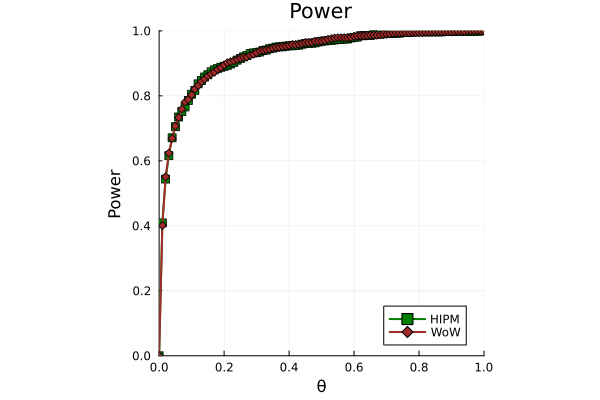
\includegraphics[width = \linewidth]{chapters/two-sample-testing/figures/wow_vs_hipm/tp_label_1=1_label_2=1_n=100_m=100_S=1000_n_perm=100.png}
        \caption{Case A}
    \end{subfigure}
    \begin{subfigure}{0.49\textwidth}
        \centering
        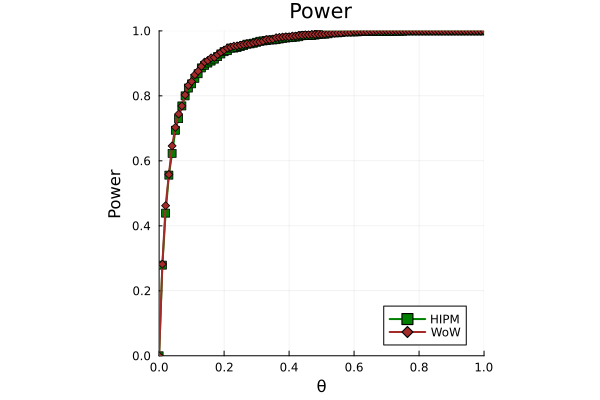
\includegraphics[width = \linewidth]{chapters/two-sample-testing/figures/wow_vs_hipm/tp_label_1=2_label_2=2_n=100_m=100_S=1000_n_perm=100.png}
        \caption{Case B}
    \end{subfigure}
    \begin{subfigure}{0.49\textwidth}
        \centering
        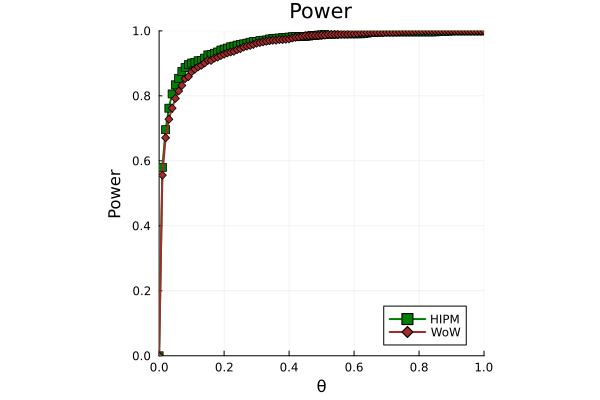
\includegraphics[width = \linewidth]{chapters/two-sample-testing/figures/wow_vs_hipm/tp_label_1=3_label_2=3_n=100_m=100_S=1000_n_perm=100.png}
        \caption{Case C}
    \end{subfigure}
    \begin{subfigure}{0.49\textwidth}
        \centering
        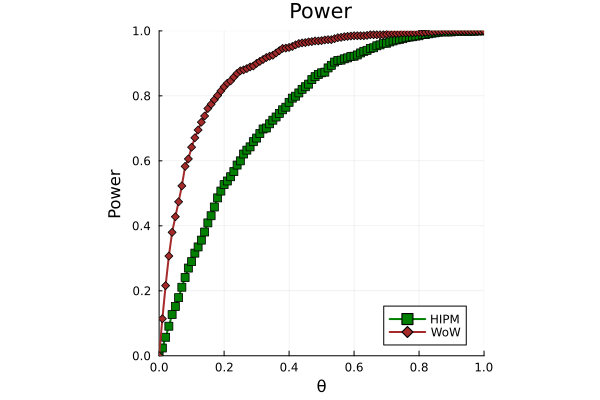
\includegraphics[width = \linewidth]{chapters/two-sample-testing/figures/wow_vs_hipm/tp_label_1=4_label_2=4_n=100_m=100_S=1000_n_perm=100.png}
        \caption{Case D}
    \end{subfigure}
    \caption{Power for WoW and HIPM}
    \label{figure:tp_wow_vs_hipm}
\end{figure}

The results presented in Figure~\ref{figure:tp_wow_vs_hipm} indicate that HIPM and WoW achieve comparable power in Cases A and B. In Case C, HIPM exhibits slightly higher power than WoW. A more pronounced difference emerges in Case D, where WoW achieves substantially higher power than HIPM. Understanding the conditions under which one method dominates the other remains an open question. One possible direction is to examine the signal-to-noise ratio of the underlying testing problem.


\subsection{Empirical comparison with existing methods}\label{subsection:comparison_of_all_methods}

Several frameworks for two-sample testing in general metric spaces have been developed in the literature. As $(\probx, \W)$ is a metric space, those methods can be specialized to that setting. We benchmark our proposed scheme against two existing methods. The first is that of \cite{dubey2019frechet}, which we refer to as the Fr\'echet test. The second is the Energy test introduced in \cite{szekely2004testing}.

The Fr\'echet test uses the concepts of Fr\'echet mean and variance for random probability measures. Recall that the mean of a real-valued random variable $X$ is the number $a \in \R$ such that
\[
a = \argmin_{a' \in \R}\E (X-a')^2.
\]
This characterization generalizes to a general metric space. In the space $(\probx,\W_2)$, the analogous notion is referred to as the Fr\'echet mean, defined as
\begin{definition}[Fr\'echet Mean]
\label{definition:Frechet_mean}
Let $Q \in \probprobx$. The Fr\'{e}chet mean is the probability measure $\mu_{F} \in \probxtwo$ defined as
\[
\mu_{F} = \argmin_{P \in \probxtwo} \E_{\widetilde{P}\sim Q} \left[\W^2_2(P, \widetilde{P})\right].
\]
\end{definition}
Accordingly, we describe the dispersion around that point, which is referred to as the Fr\'echet variance.
\begin{definition}[Fr\'echet Variance]
\label{definition:Frechet_variance}
Let $Q \in \probprobx$. The Fr\'echet variance $V_{F}$ is defined as
\[
V_{F} = \min_{P \in \probxtwo}\E_{\widetilde{P}\sim Q} \left[\W^2_2(P, \widetilde{P})\right] 
= \E_{\widetilde{P}\sim Q} \left[\W^2_2(\mu_F, \widetilde{P})\right]
\]
\end{definition}
The asymptotic theory of the Fr\'echet test is developed for bounded metric spaces under additional regularity assumptions. In the case of $\probx$, these assumptions are known to hold when the Wasserstein distance is of order $2$ and $\X$ is a compact interval of the real line. It is important to note that the Fr\'echet test targets the surrogate null hypothesis of equality of Fr\'echet means and Fr\'echet variances associated to laws of random probability measures.


The Energy test was first developed as a testing procedure for samples taking values in Euclidean spaces. It can be extended to a general metric space $(\Y,d)$, provided that the underlying space is of strongly negative type (see \cite{lyons2013distance} for a comprehensive overview).

We compare the methods in two different scenarios using the same baseline as \cite{dubey2019frechet}. In each scenario, we examine the rejection rates of each testing scheme for several pairs of laws of random probability measures. The random probability measures we consider are
\begin{equation}\label{equation:tnormal_normal_model}
\tilde P^i| \tilde \mu^{(i)} = \mathcal{N}(\tilde \mu^{(i)}, 1), \qquad \tilde \mu^{(i)} \sim  \mathcal{N}_T(\mu_{0i}, \sigma^2_{0i} , a, b),
\end{equation}
for $i = 1,2$, where $\mathcal{N}_T (\cdot, \cdot, a,b)$ denotes the truncated normal distribution on $[a,b]$. To obtain the set of pairs, we vary a parameter governing the random means. In particular, we consider the following settings:
\begin{enumerate}
\item The difference between two distributions is dictated by changing the mean parameter of the random mean, reproducing the setting of Figure~1 in \cite{dubey2019frechet}, where $Q^i$ are as in \eqref{equation:tnormal_normal_model} with $\sigma_{01} = \sigma_{02} = 0.5$, $a = -10$, $b = 10$ and
\[
\mu_{01} = 0, \qquad \mu_{02} = \delta, \qquad \delta \in [-1, 1]. 
\]
\item The difference between two distributions is dictated by changing the variance parameter of the random mean, reproducing the setting of Figure~1 in \cite{dubey2019frechet}, where $Q^i$ are as in \eqref{equation:tnormal_normal_model} with $\mu_{01} = \mu_{02} = 0$, $a = -10$, $b = 10$ and
\[
\sigma_{01} = 0.2, \qquad \sigma_{02} = 0.2\tau, \qquad  \tau \in [0, 3].
\]
\end{enumerate}
A low type I error is reflected by a low rejection rate under $H_0$, corresponding respectively to $\delta = 0$ and  $\tau = 1$. High power is reflected by a steep increase in the rejection curve away from $H_0$.

For each setting we simulate the data $S=1000$ times, perform all tests on the same data, and report the percentage of times they reject the corresponding null hypothesis. We set the hierarchical sample sizes to $n = 100$, $m = 200$. Our tests use a permutation approach with $n_{\text{perm}} = 100$ re-samples, while the Fr\'echet test uses a bootstrap approach with $n_{\text{boot}} = 100$ re-samples. For the Fr\'echet test, we work directly with samples from the Gaussian distributions rather than hierarchical samples. Results are reported in Figure~\ref{figure:rejections_mean_variance}.
\begin{figure}[H]
    \centering
    \begin{subfigure}{0.49\textwidth}
        \centering
        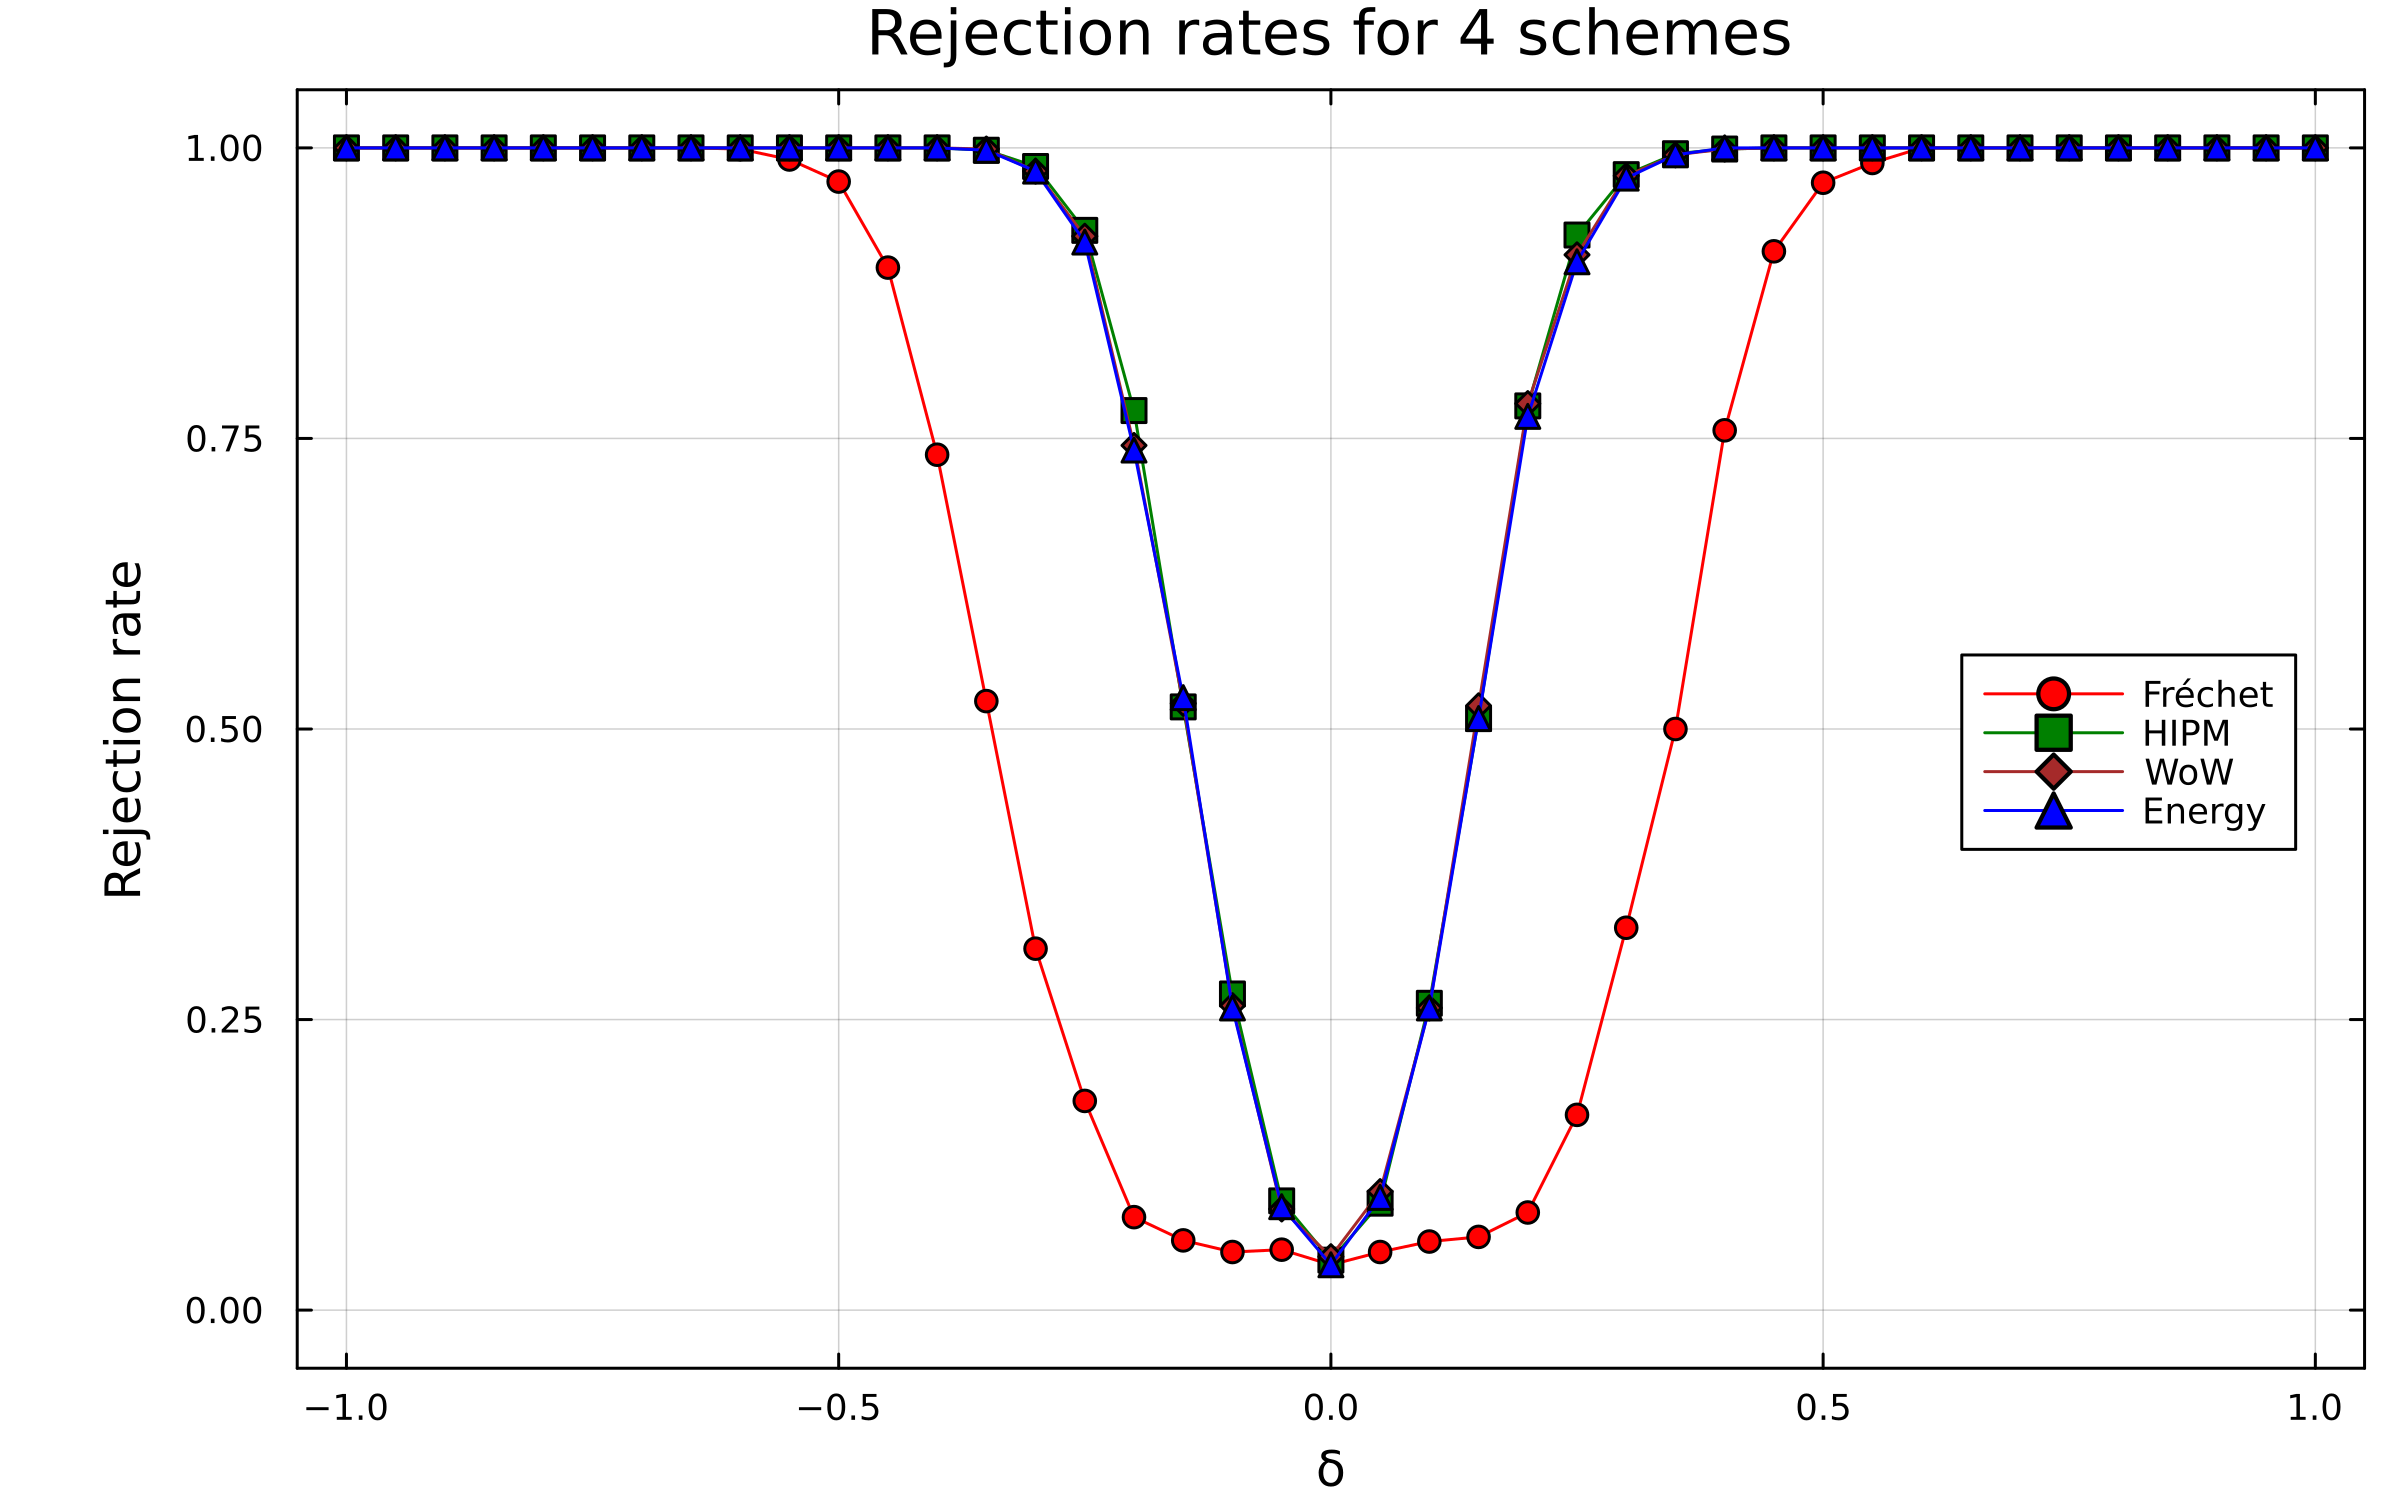
\includegraphics[width = \linewidth]{chapters/two-sample-testing/figures/all_schemes/mean_n=100_m=200_S=1000_bootstrap=false_n_samples=100.png}
    \end{subfigure}
    \begin{subfigure}{0.49\textwidth}
        \centering
        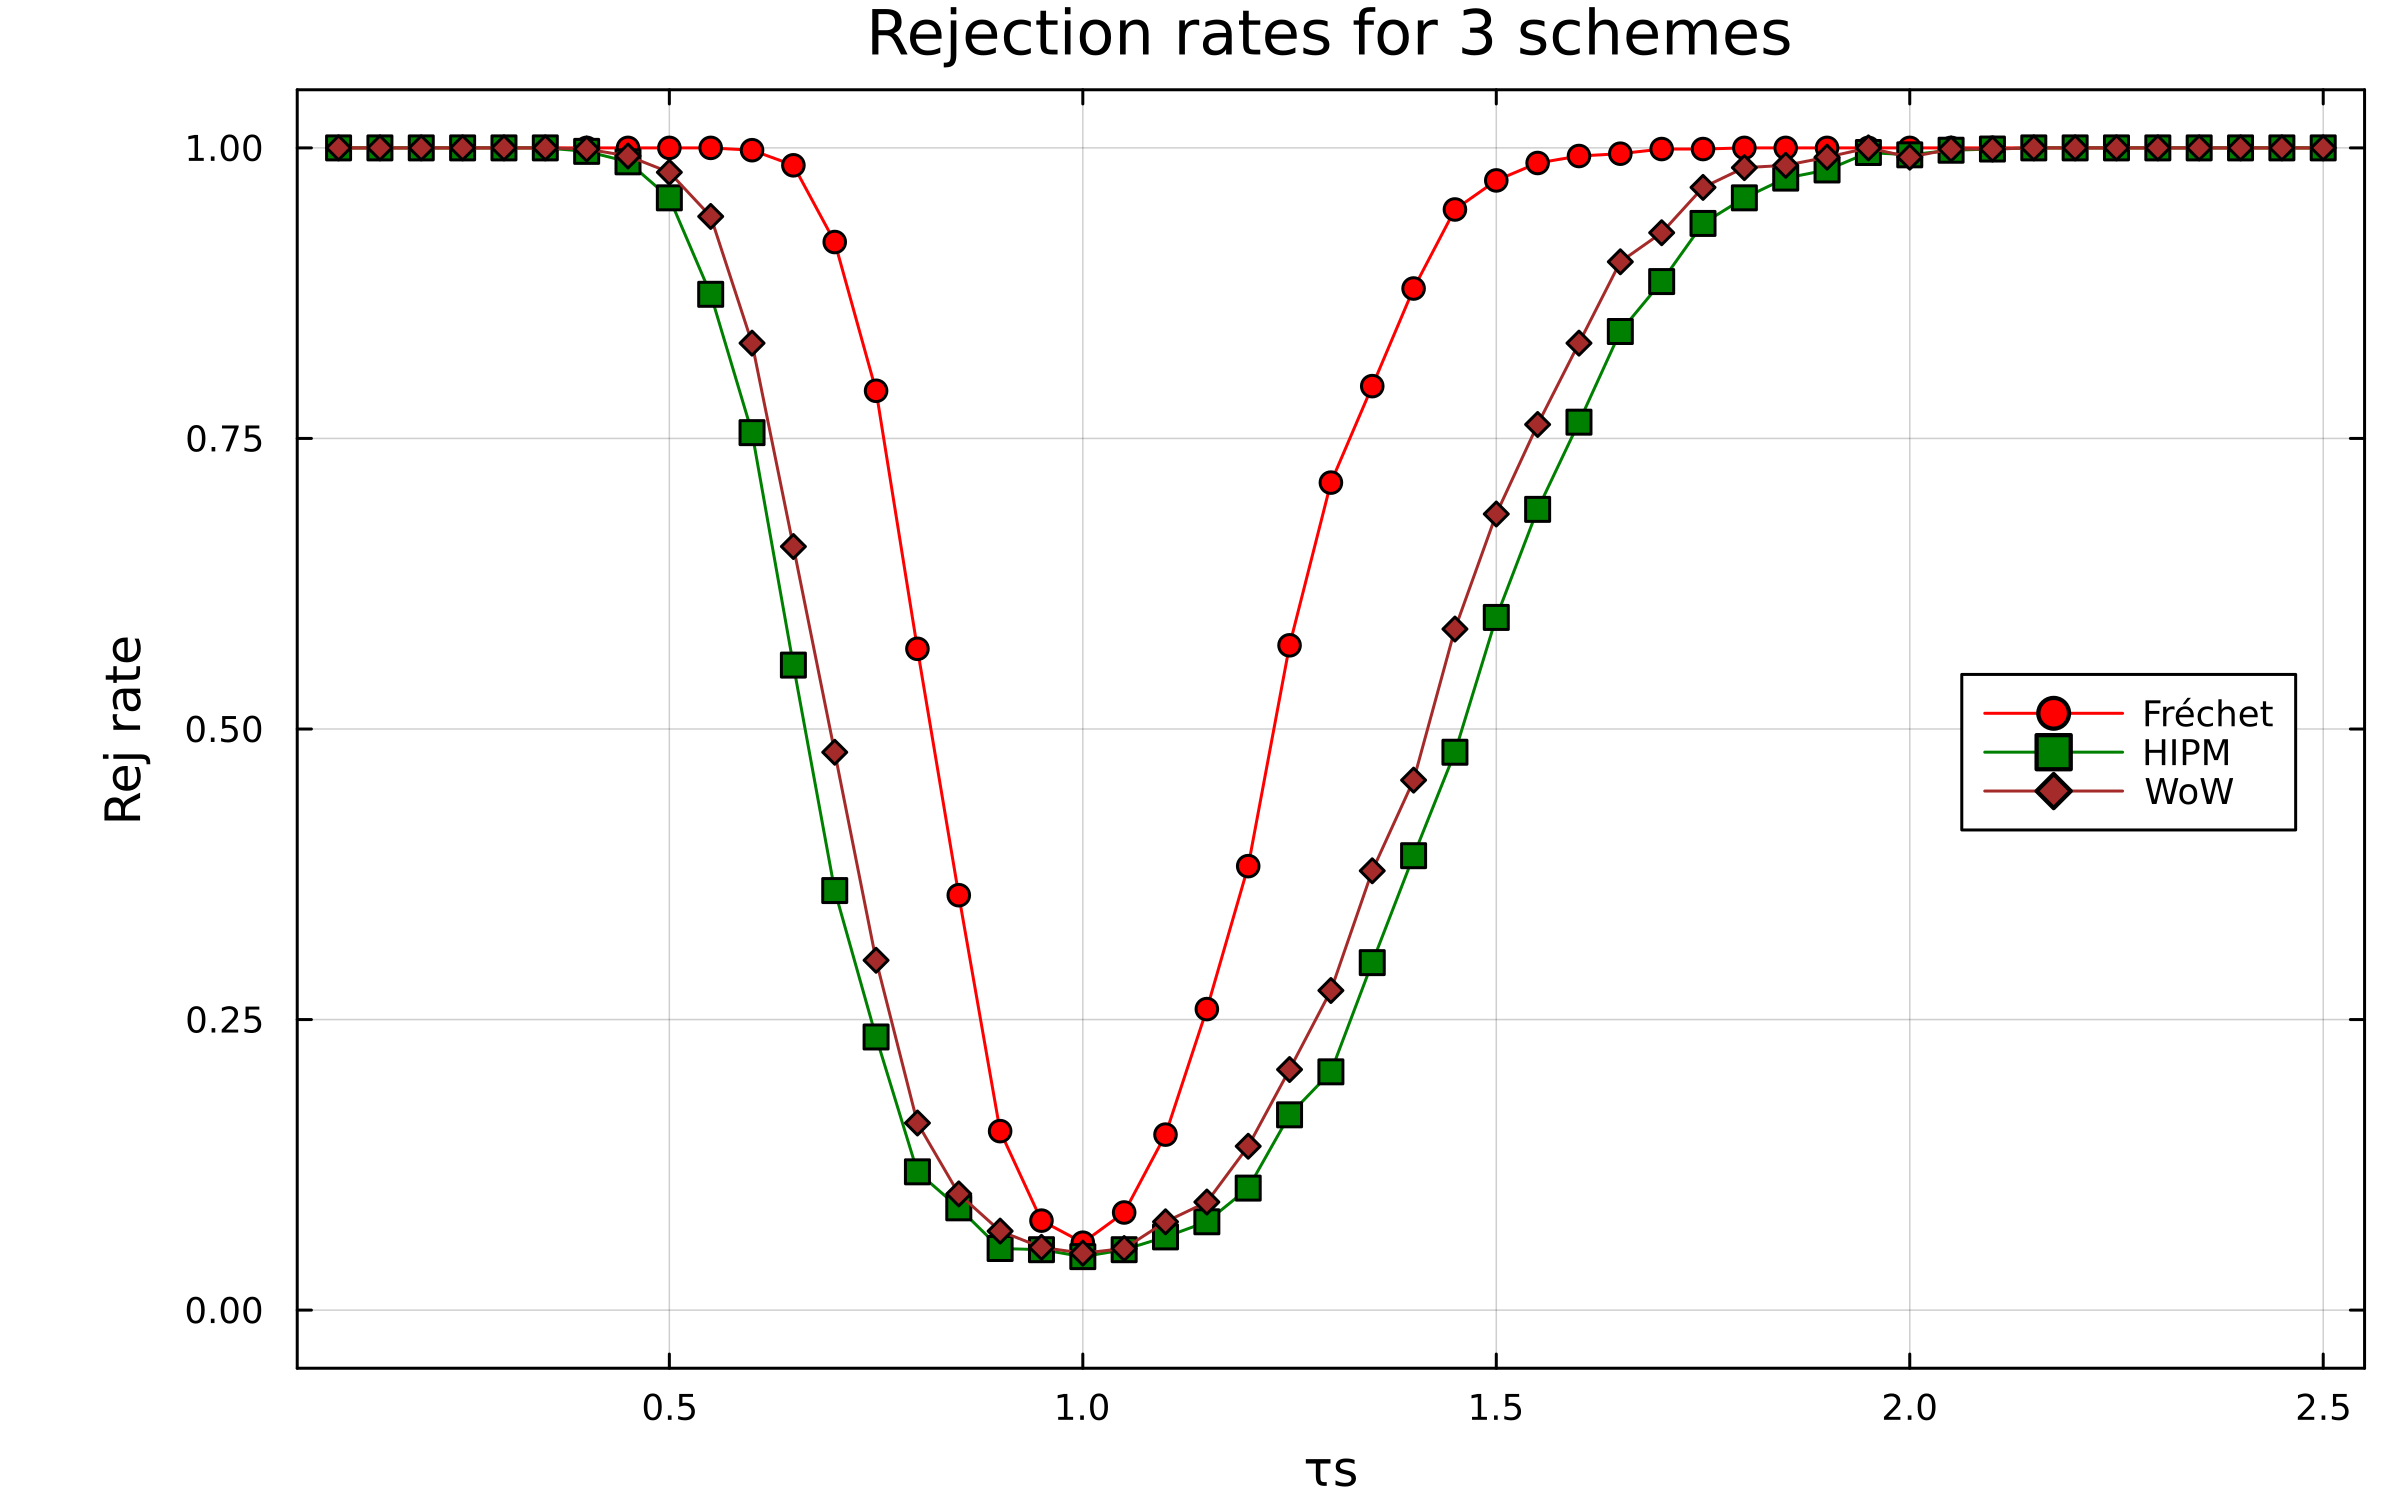
\includegraphics[width = \linewidth]{chapters/two-sample-testing/figures/all_schemes/variance_n=100_m=200_S=1000_bootstrap=false_n_samples=100.png}
    \end{subfigure}
    \caption{Rejection rates for WoW, HIPM, Fr\'echet and Energy tests}
    \label{figure:rejections_mean_variance}
\end{figure}
As seen in Figure~\ref{figure:rejections_mean_variance}, all testing schemes maintain low Type I error across both settings. When the distributions differ in mean (left plot), the Energy, WoW, and HIPM tests achieve higher power than the Fr\'echet test. In contrast, when the distributions differ in variance (right plot), the Fr\'echet test attains the highest power among all methods. Furthermore, in the variance setting, both HIPM and WoW outperform the Energy test.


The final simulation on the synthetic dataset is designed to demonstrate the necessity of distance-based testing. Note that the underlying assumption behind the Fr\'echet test is that the Fr\'echet mean and variance are sufficient to distinguish between two different laws of random probability measures. However, laws of RPMs are not always uniquely characterized by their Fr\'echet means and variances.

Indeed, we can construct a simple counterexample. Consider
\begin{align*}
   &Q^1 = \law\widetilde{P}^1 \quad \text{where} \quad \widetilde{P}^1 | \tilde{\mu} = \N\left( \widetilde{\mu}^1, 1\right), \quad \widetilde{\mu}^1 \sim \tfrac{1}{2}\delta_{-1} + \tfrac{1}{2}\delta_{1}, \\
   &Q^2 = \law \widetilde{P}^2 \quad \text{where} \quad \widetilde{P}^2 | \tilde{\mu}  = \N\left( \widetilde{\mu}^2, 1\right), \quad \widetilde{\mu}^2 \sim  \tfrac{1}{8}\delta_{-2} + \tfrac{3}{4}\delta_{0} + \tfrac{1}{8}\delta_{2},
\end{align*}
where $Q^1 \neq Q^2$, yet their associated Fr\'echet means and variances coincide (see Remark~\ref{remark:frechet_mean_variance_special_case_variance_1}).

Moreover, if we compare $Q^1$ with a mixture of $Q^1$ and $Q^2$, the resulting laws remain different while still inducing the same Fr\'echet means and variances (see Remark~\ref{remark:frechet_mean_variance_mixture_of_laws}). Specifically, letting
\[
M_\lambda = \lambda Q^1 + (1-\lambda)Q^2,
\]
we consider the family of pairs
\[
\{(Q^1, M_\lambda) : \lambda \in [0,1]\}.
\]
Note that $\lambda = 1$ corresponds to estimating the Type~I error, while other values of $\lambda$ correspond to estimating the power of the testing procedures. We consider mixtures of the two laws because, as the parameter varies, it becomes more challenging for the testing schemes to detect the presence of different laws. We plot the rejection rates in Figure~\ref{figure:counterexample}, where the simulation parameters are the same as those used in Figure~\ref{figure:rejections_mean_variance}.
\begin{figure}[H]
    \centering
    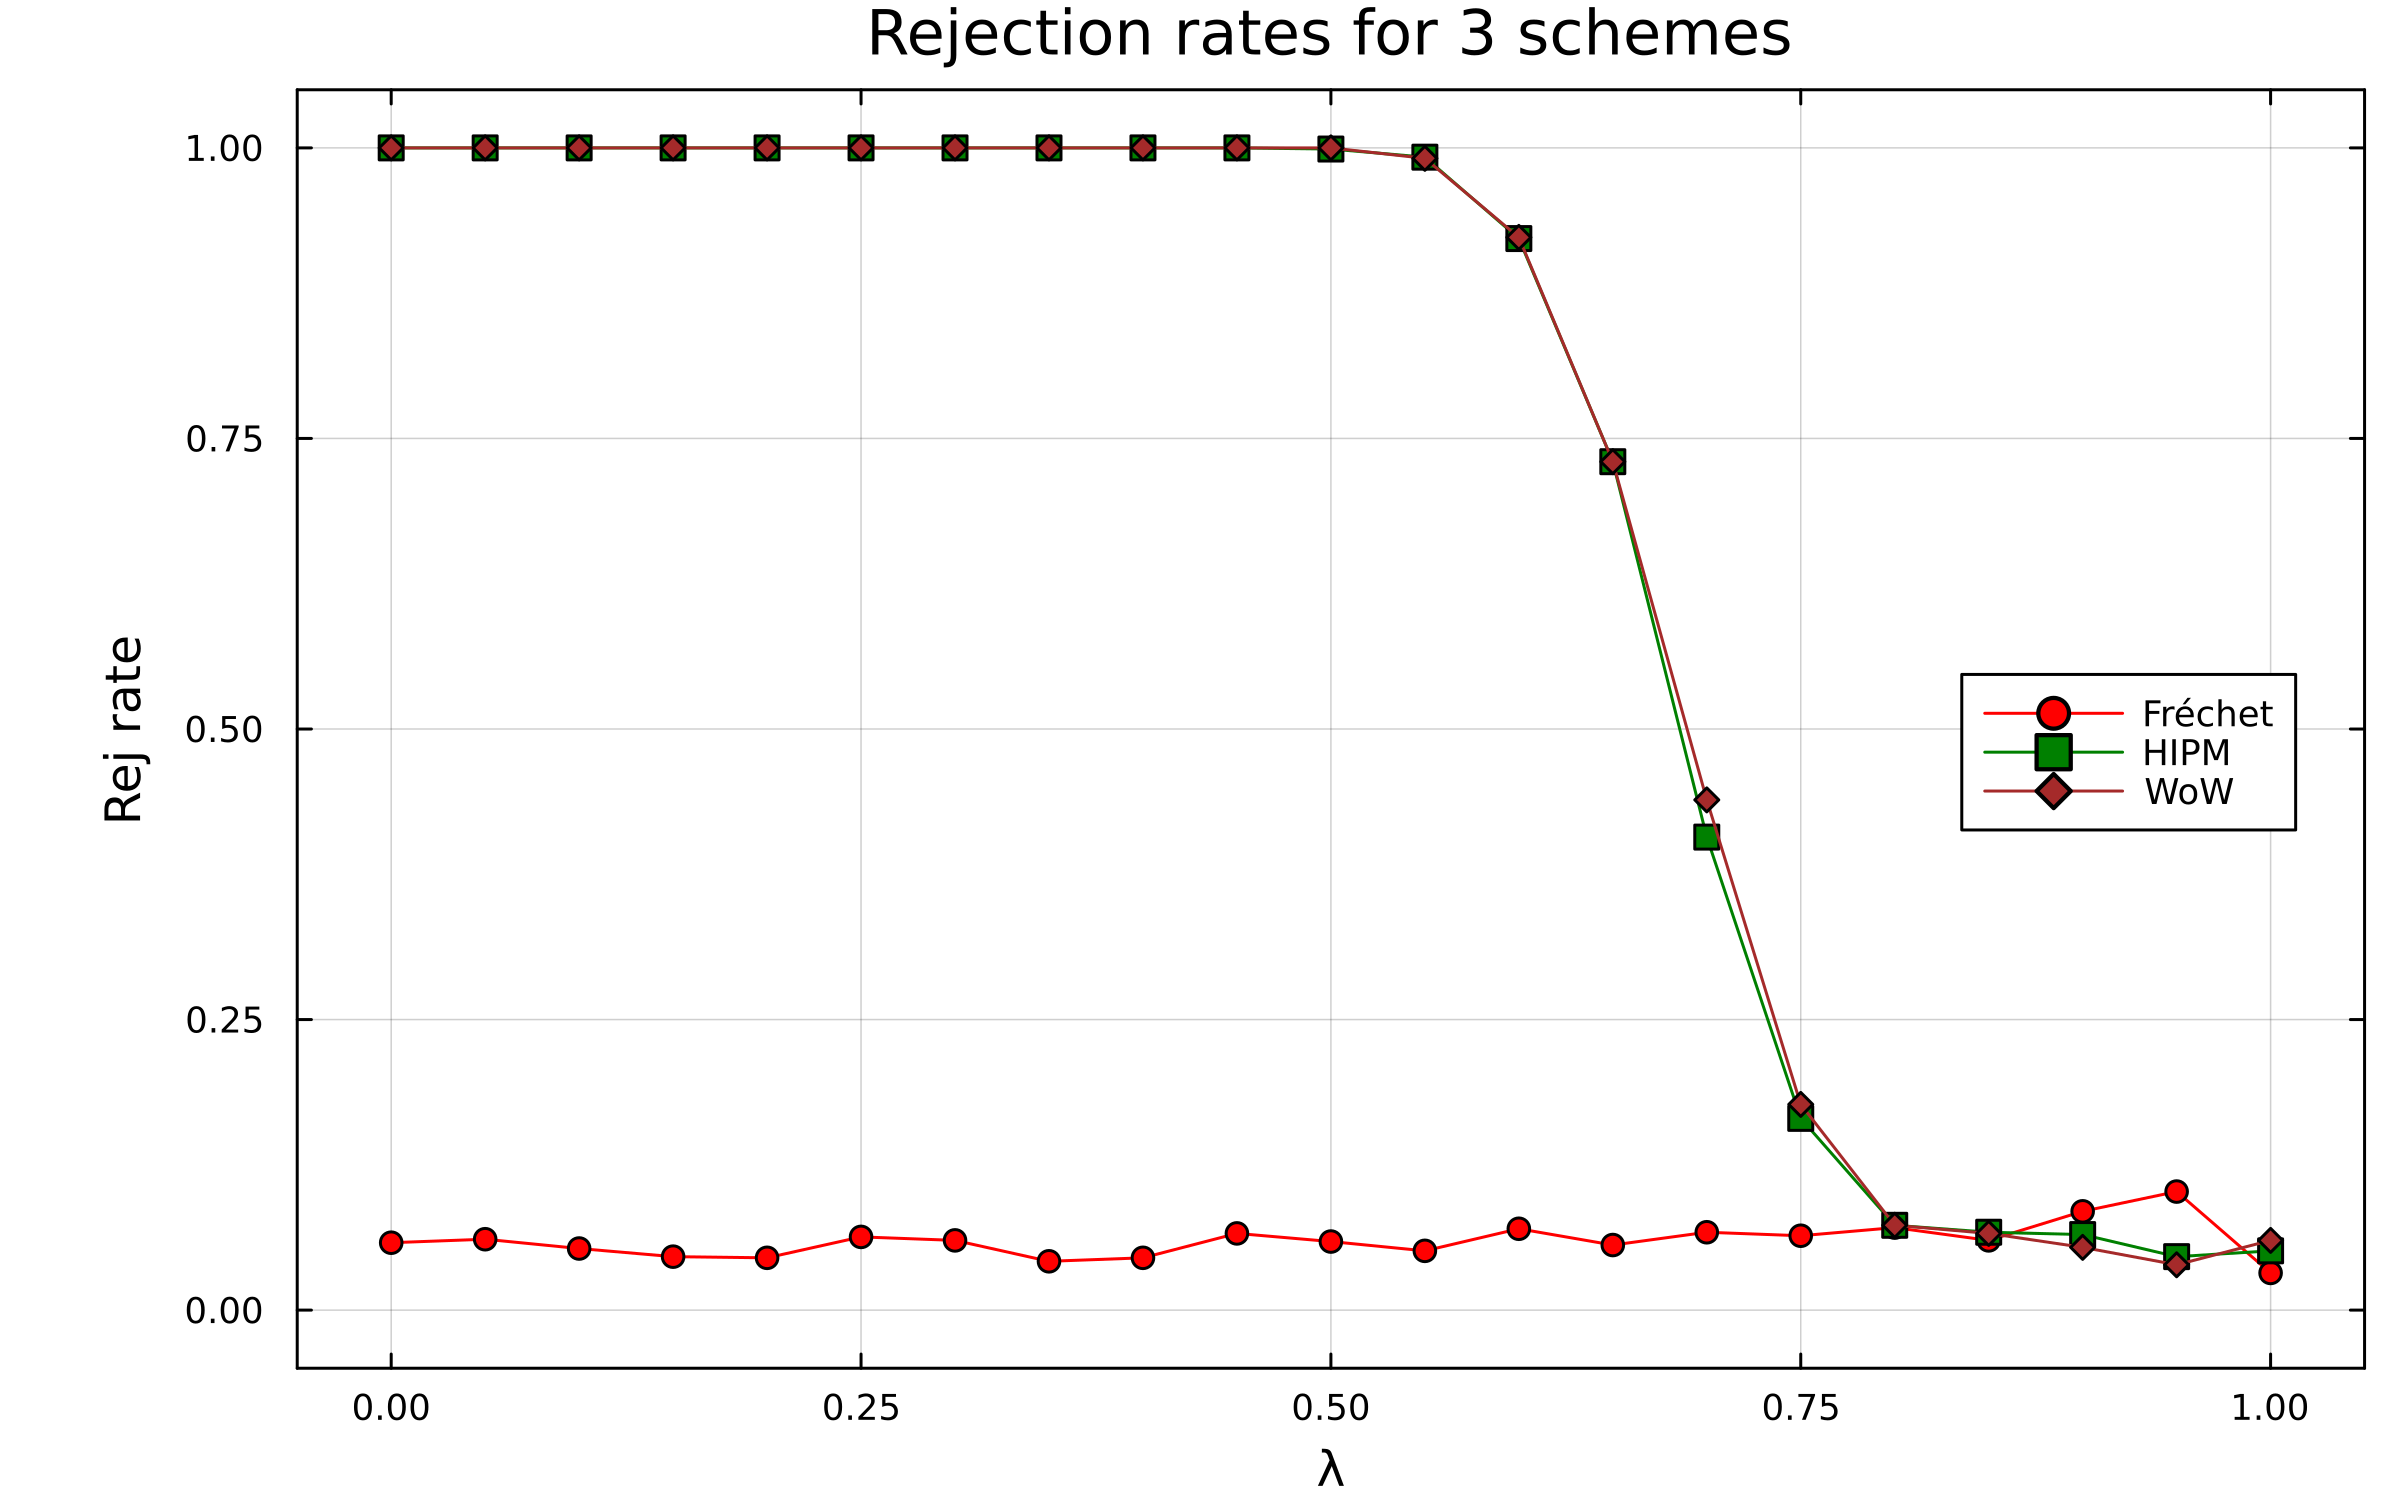
\includegraphics[width=0.43\textwidth]{chapters/two-sample-testing/figures/all_schemes/counterexample_n=100_m=200_S=1000_bootstrap=false_n_samples=100.png}
    \caption{Rejection rates for WoW, HIPM, Fr\'echet and Energy tests}
    \label{figure:counterexample}
\end{figure}

As observed in Figure~\ref{figure:counterexample}, since the two distributions induce the same Fr\'echet means and variances, the method proposed in \cite{dubey2019frechet} fails to detect the presence of different laws. In contrast, the HIPM and WoW tests perform slightly better than the Energy test in identifying the discrepancy.

To conclude, although the Fr\'echet test can exhibit higher power than the other testing schemes in certain settings, its main limitation is that it fails to detect the difference when the laws of random probability measures are not fully characterized by the Fr\'echet mean and variance. The Energy test, as well as permutation tests based on HIPM or WoW, mitigate this limitation. Moreover, HIPM and WoW may be preferable to the Energy test in practice, since the underlying metric space, in our case, the space of probability measures, may fail to be of strongly negative type, or this property may be difficult to verify.


\subsection{Mortality Data}\label{subsection:mortality_data}

We apply our proposed testing scheme to human mortality data obtained from the Human Mortality Database (https://www.mortality.org/). The dataset contains period life tables for various countries and calendar years. A period life table summarizes mortality conditions in a given calendar year by describing how a hypothetical cohort would die if it faced the age-specific mortality proportions observed in that year. The resulting mortality proportions are then used to derive the age-at-death distribution of the hypothetical cohort.

Our analysis compares mortality proportions from 1960 to 2010 between two historically motivated groups of countries. Following the classification in \cite{dubey2019frechet}, the first group consists of countries that were either part of the Soviet Union or belonged to the Soviet-aligned Eastern Bloc during much of the 20th century. The second group consists mainly of Western or non-Soviet high-income countries, including several countries that were politically neutral during the Cold War.
\begin{itemize}
    \item Group 1 : Belarus, Bulgaria, Czechia, Estonia, Hungary, Latvia, Lithuania, Poland, Russia, Slovakia, and Ukraine.
    \item Group 2 : Australia, Austria, Belgium, Canada, Denmark, Finland, France, Iceland, Ireland, Italy, Japan, Luxembourg, Netherlands, New Zealand, Norway, Spain, Sweden, Switzerland, United Kingdom, and United States of America.
\end{itemize}
The age range is $\{0,1,\cdots,110\}$, where $110$ denotes that death occurred at that age or later. We choose not to truncate the age range for the following reasons. First, visual inspection of the probability mass functions and quantiles does not reveal any abnormalities, particularly at higher ages (see Figure~\ref{figure:quantile_for_mortality_rates}). Second, truncating the age range leads to significant data loss. For example, among females, the maximum percentage of data lost across countries is at least $20$ percent for all time periods when the age interval is truncated to $\{0,1,\dots,85\}$.

In Figure~\ref{figure:quantile_for_mortality_rates}, we present the quantile plots of the probability mass functions corresponding to age at death for both males and females. We consider the years 1960, 1992, and 2008 to capture different historical periods: the Cold War era closer to the post-war period, the years shortly after the collapse of the Soviet Union, and a more recent period following the breakup. The plots are shown separately for females and males. As observed, noticeable differences can be visually identified, particularly in the more recent time periods.
\begin{figure}[htbp]
    \centering
    \begin{subfigure}{0.5\textwidth} % Increased width since they are stacked
        \centering
        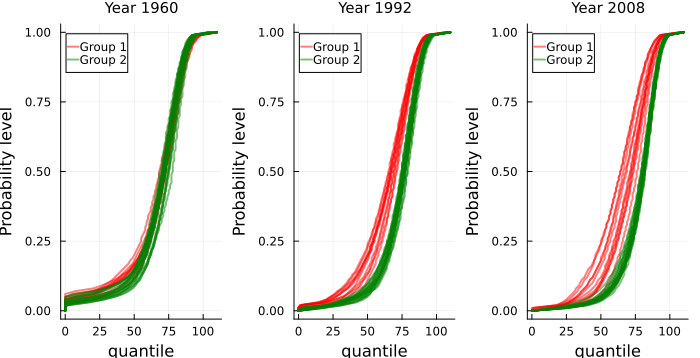
\includegraphics[width=\linewidth]{chapters/two-sample-testing/figures/mortality/males_allquantiles_0_110.png}
        \caption{Males}
    \end{subfigure}
    \\ % <--- This line break forces the next subfigure down
    \begin{subfigure}{0.5\textwidth}
        \centering
        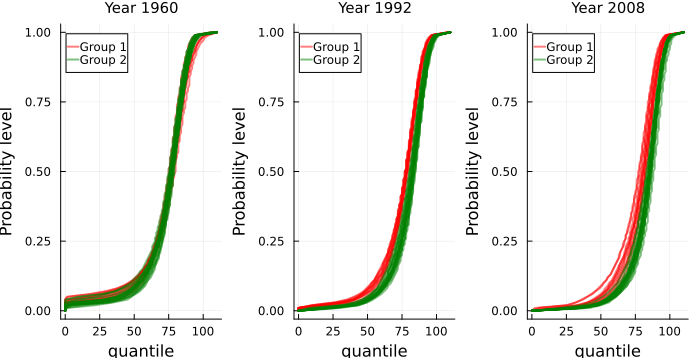
\includegraphics[width=\linewidth]{chapters/two-sample-testing/figures/mortality/females_allquantiles_0_110.png}
        \caption{Females}
    \end{subfigure}
    \caption{Quantile plots of the age-at-death probability mass functions for the two country groups}
    \label{figure:quantile_for_mortality_rates}
\end{figure}
To assess whether there is a difference in mortality proportions between the two groups of countries in each time period, we apply tests using HIPM and WoW separately for males and females. We set the significance level to $\theta = 0.05$ and use $n_{\text{perm}} = 100$ permutations to compute a p-value for each year.

We also compare the p-values obtained from our approach with those derived from the following alternative methods:
\begin{itemize}
\item Averaging: Given $\widehat{P}^1_1,\cdots, \widehat{P}^1_{n_1}$ from group 1 and $\widehat{P}^2_1,\cdots, \widehat{P}^2_{n_2}$ from group 2, we obtain average probability measures inside each group, i.e.
\[
\overline{P}^1 = \frac{1}{n_1}\sum_{i = 1}^{n_1}\widehat{P}^1_i, \quad
\overline{P}^2 = \frac{1}{n_2}\sum_{i = 1}^{n_2}\widehat{P}^2_i.
\]
The test statistic is obtained by computing Wasserstein-1 distance between $\overline{P}^1$ and $\overline{P}^2.$ The threshold is obtained via a permutation approach, in which the observed probability measures are permuted across the two groups.
\item Pooling: This approach is included to emphasize the importance of preserving the probability-measure structure within each group. Since the goal is to compare mortality proportions across the two groups, one might instead ignore the country-level distributional structure and simply aggregate deaths within each group. This aggregation produces a single probability measure for each group, and the test statistic is then computed as the Wasserstein-1 distance between these two measures. As before, the significance threshold is obtained using a permutation procedure. Because the data for each country consist of death counts by age, we first convert these counts into observations of age at death. Specifically, if there are $k$ deaths at age $a$, we generate $k$ observations equal to $a$. This is done separately for each group. The resulting age-at-death observations are then permuted across the two groups, which allows the permutation procedure to operate directly on individual age-at-death observations rather than on aggregated counts.
\end{itemize}
Note that the test statistic is identical for both the pooling and averaging approaches; the difference between the two testing schemes lies in the permutation procedure. In particular, the averaging approach preserves the probability measure structure within each group, whereas the pooling approach does not.

Examining the p-values from all methods in Figure~\ref{figure::p_values_mortality}, we observe that for females, the difference between the groups is statistically significant in 1960. During the following decade, this difference becomes less significant under the methods based on HIPM, WoW, and Averaging, which may be explained by economic growth. After the 1970s, the disparity in mortality proportions between the groups increases again, potentially reflecting the economic decline in the countries of Group~1. Following the breakup of the Soviet Union, the observed differences may be associated with countries that were unable to integrate well into the Western bloc.

A similar trend is observed for males; however, the key difference is that during the period from 1960 to 1970, although the differences in mortality proportions were decreasing, this was not statistically significant in all of those years.
\begin{figure}[htbp]
    \centering
    \begin{subfigure}{0.5\textwidth} % Increased width since they are stacked
        \centering
        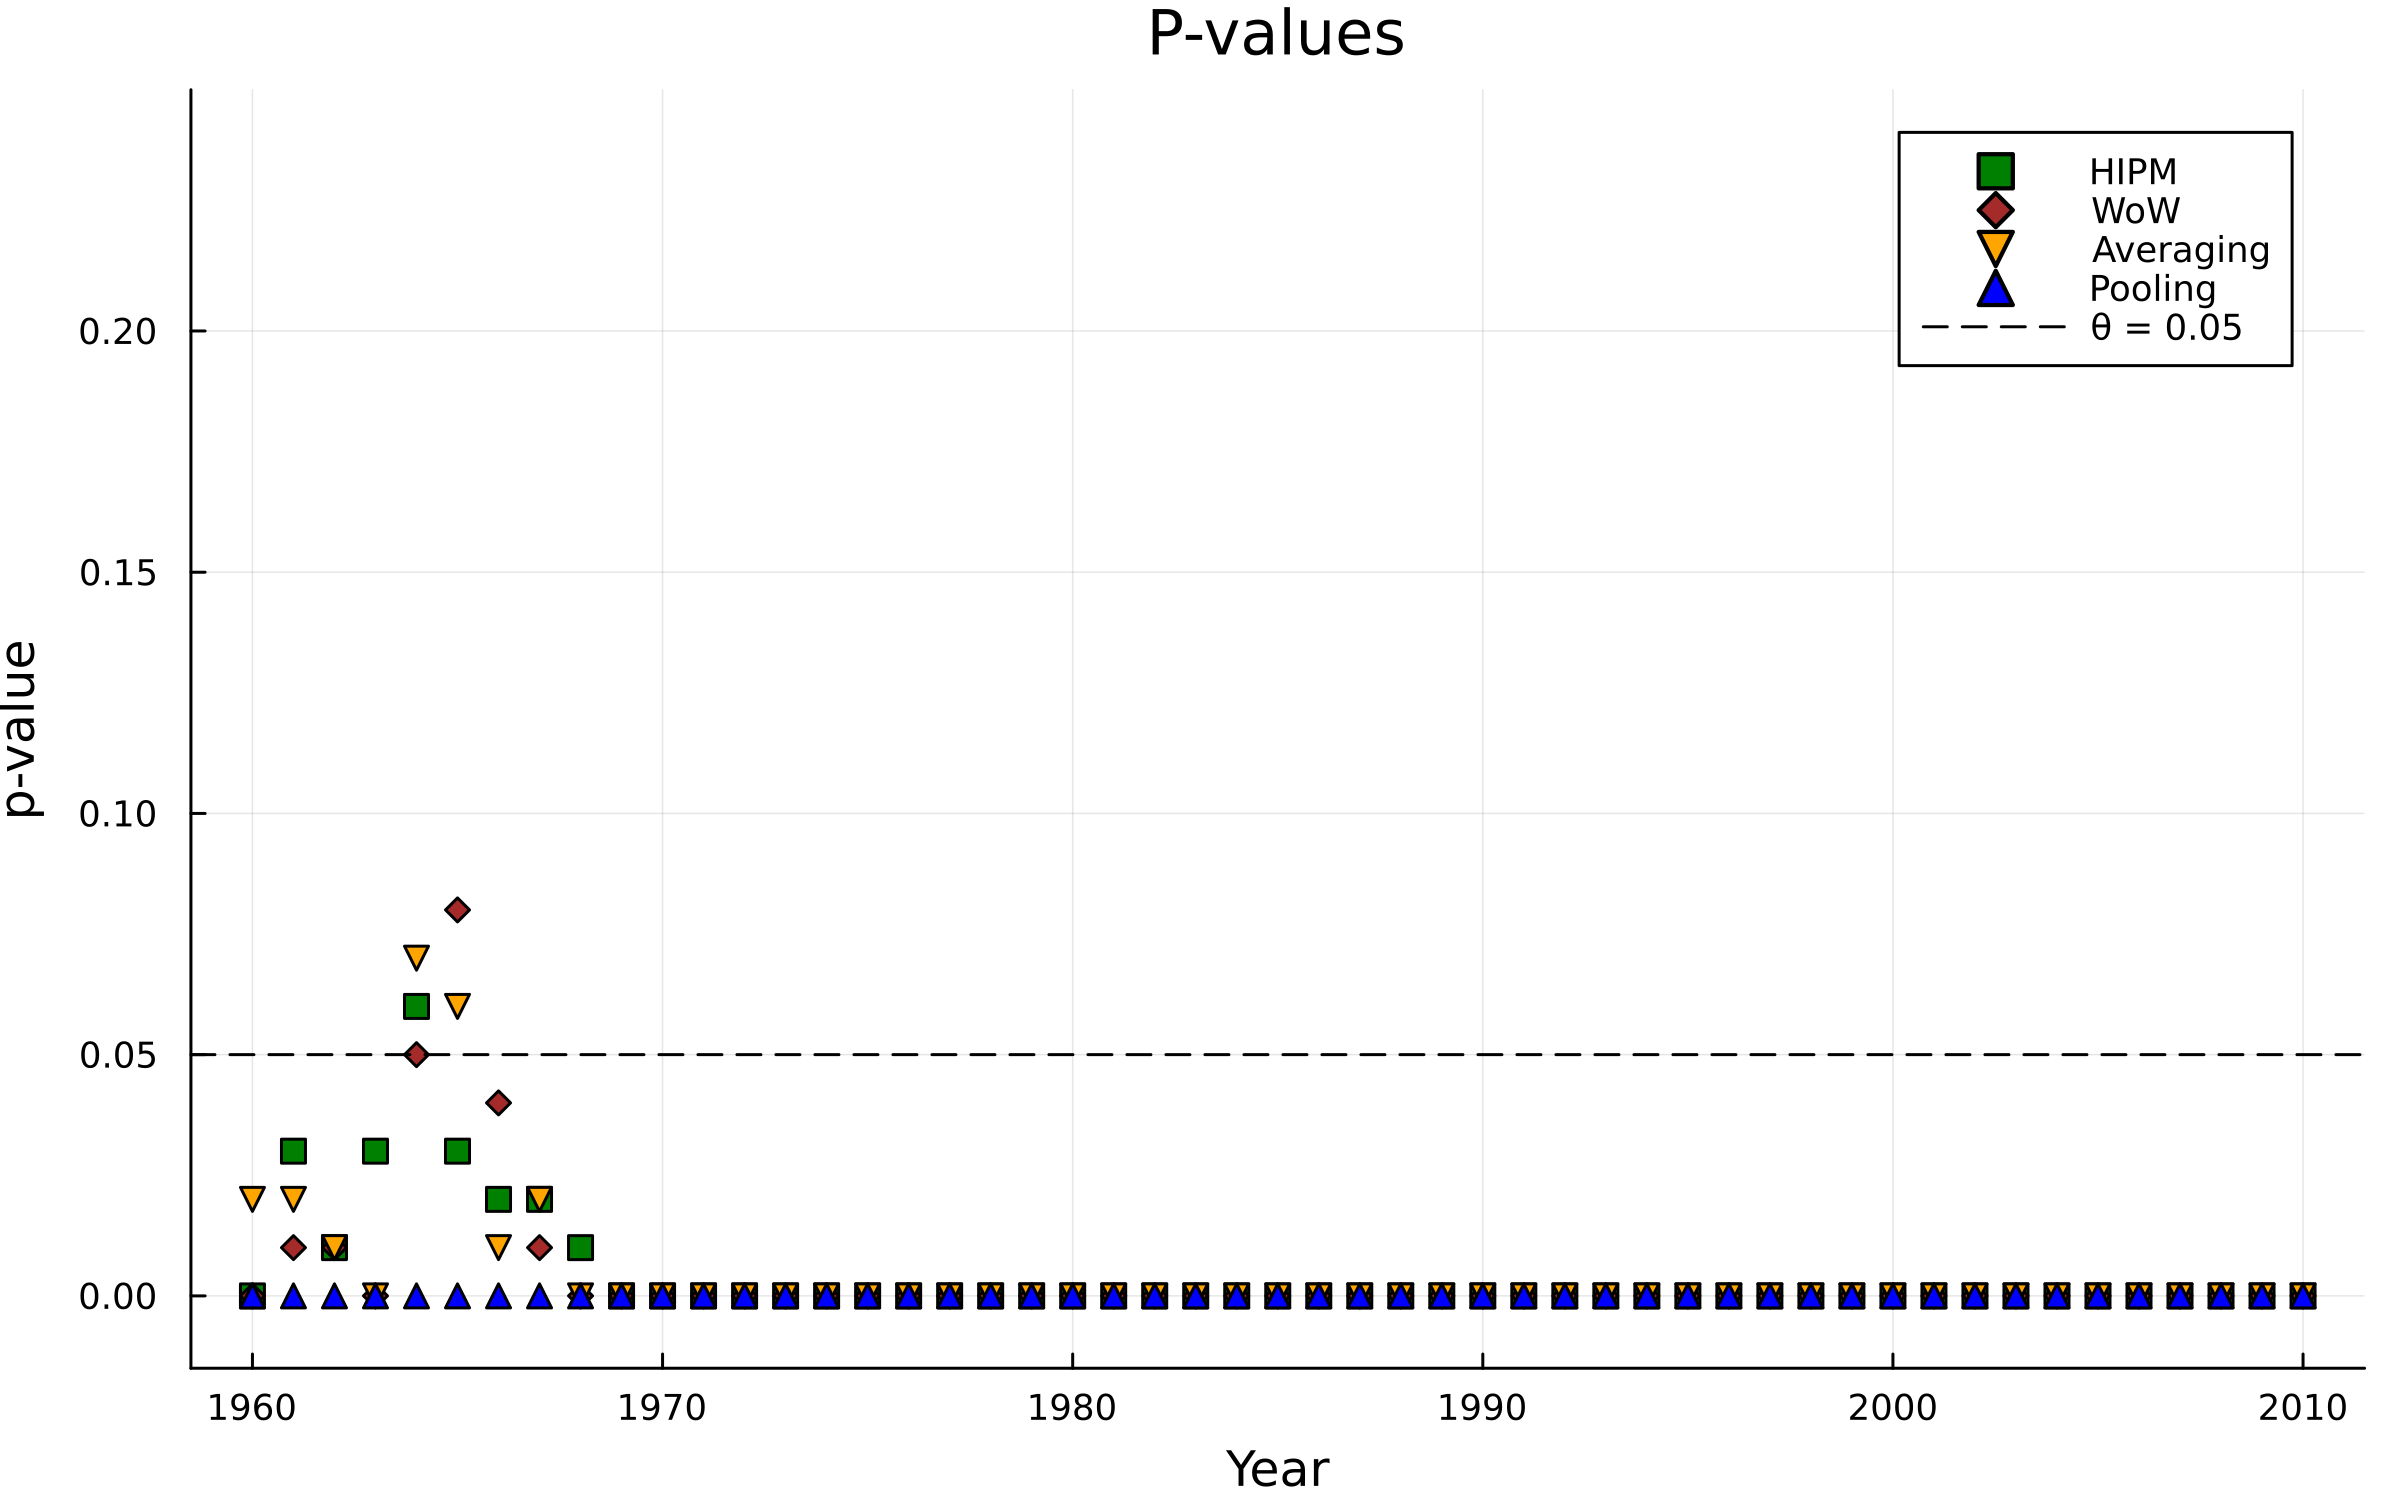
\includegraphics[width=\linewidth]{chapters/two-sample-testing/figures/mortality/pvalues_males.png}
        \caption{Males}
    \end{subfigure}
    \\ % <--- This line break forces the next subfigure down
    \begin{subfigure}{0.5\textwidth}
        \centering
        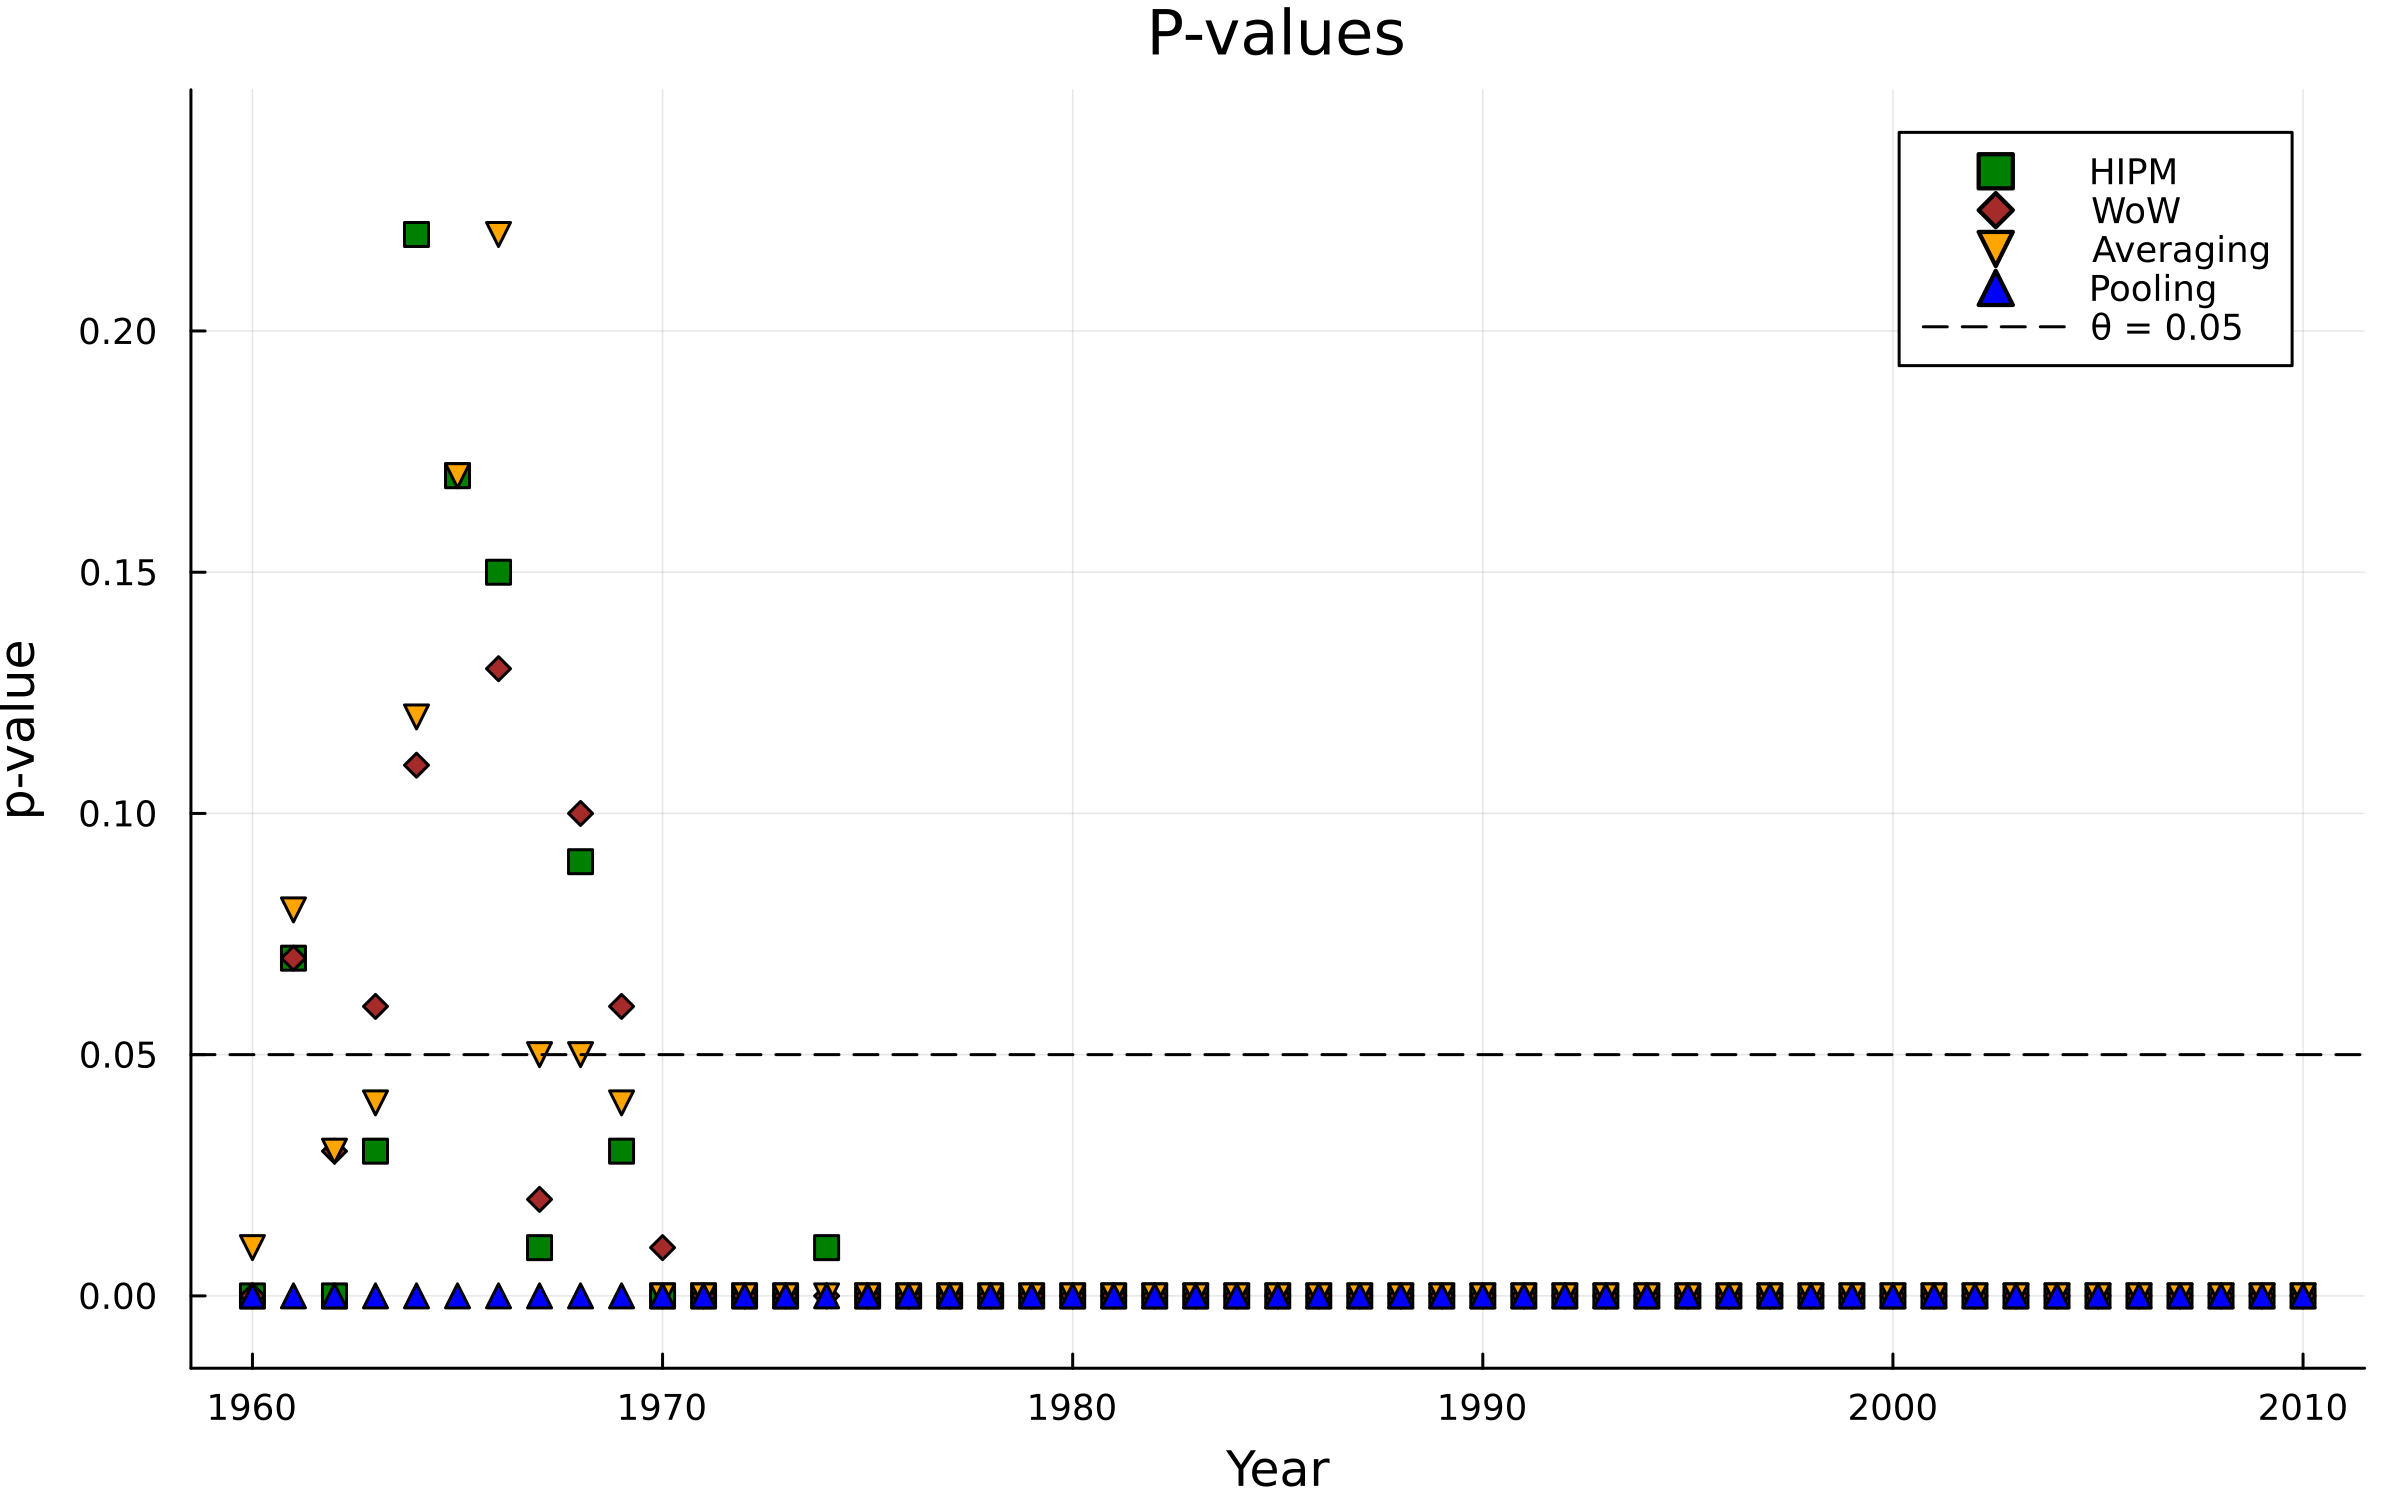
\includegraphics[width=\linewidth]{chapters/two-sample-testing/figures/mortality/pvalues_females.png}
        \caption{Females}
    \end{subfigure}
    \caption{P-values for mortality proportions}
    \label{figure::p_values_mortality}
\end{figure}

Note also that the p-values for Averaging, HIPM, and WoW follow a similar trend. This is because the average measure is in this case sufficient to detect the difference between the two groups.


We also observe an important issue concerning the pooling approach, which is of broader relevance to hierarchical sampling settings. In particular, the pooling procedure may fail to control the Type I error in hierarchical sampling settings. This is because pooling ignores the fact that observations within each country are generated from a latent random probability measure. Under hierarchical sampling, where we observe $n$ sequences of length $m$, each generated from a different latent random probability measure, the empirical distribution obtained by pooling all observations converges to the mean measure of the law of the random probability measure. Hence, the pooled test statistic converges to the Wasserstein distance between the two group-level mean measures. In contrast, the permutation samples behave as if they were drawn directly from this mean measure, with an effective sample size of $nm$. As a result, the permutation threshold converges to zero faster than the observed distance, leading to systematically small p-values. This issue disappears when the latent probability measures are identical.











        
        


        
      


        
       


        









\begin{subappendices}
\section{Function class for HIPM}\label{appendix:reductionD}
Recall that $(\X,d_\X)$ is a Polish space with bounded diameter $\mathrm{diam}(\X) = K.$ Recall also the definition of the function class $\D$ on which HIPM is defined.
\[
\D = \{h:\probx\to \R: h(P) = g(P(f)),  g\in\lipR, f\in \lipX \}
\]
Note that, as $g$ can be any constant function, $\D$ is not uniformly bounded. However, as we are working with Lipschitz functions and the sample space has bounded diameter, intuition suggests that we can obtain a uniformly bounded function class starting from $\D$ without changing the distance function. 

We show that after reducing the function class $\D$ to another function class $\dstar,$ where 
\begin{equation}\label{definition:dstar}
\dstar = \{h:\probx \to \R : h = g(P(f)), \ f \in \lipXstar, \ g \in \lipKzero \},
\end{equation}
with, for a fixed $x_0 \in \X$,
$$
\lipXstar = \{ f^* = f - f(x_0) : f \in \lipX \},
$$
and
$$
\lipKzero = \{ g^* = g - g(0) : g \in \lipK \},
$$
the HIPM distance is unchanged when the supremum is taken over $\dstar.$ 

Recall that 
$$
\dlip(Q^1,Q^2) = \sup_{h\in \D}\left| \int_{\probx} h(P)\,\mathrm{d}Q^1(P) - \int_{\probx} h(P)\,\mathrm{d}Q^2(P) \right|.
$$  
\begin{itemize}
    \item Step 1: Reduce $\D$ to
    \[
    \D' =  \{h : \probx \to \R : h(P) = g(P(f)) \text{ s.t. } g \in \lipR, f \in \lipXstar \}.
    \]
\end{itemize}
As $\lipX$ contains all constant functions, it is not uniformly bounded. Because of that, for a fixed $x_0 \in \X$, we consider
$$\lipXstar = \{ f^* = f - f(x_0) : f\in \lipX\}.$$
Note that the functions in $\lipXstar$ are $1$-Lipschitz, and they are uniformly bounded by $K$, because for all $f^*\in \lipXstar$,
\[
\sup_{x\in\X}|f^*(x)| = \sup_{x\in\X}|f(x) - f(x_0) |\leq \sup_{x\in \X}d_\X(x,x_0)\leq K.
\]
The question is whether the distance changes when we replace $\lipX$ by $\lipXstar.$ It therefore suffices to verify that $\D \subset \D'$, since the reverse inclusion is immediate.    

Let $h(P) = g(P(f))$ where $f\in\lipX, g\in \lipR$. Define $\widetilde{g}(x) = g(x + f(x_0))$ and $f^*(x) = f(x) - f(x_0)$. Note that $\widetilde{g}\in \lipR$, because for every $x, y \in \R,$
$$
|\widetilde{g}(x) - \widetilde{g}(y)| = |g(x+f(x_0)) - g(y+f(x_0))| \leq |(x+f(x_0)) - (y + f(x_0))| = |x-y|.
$$
Hence,
$$
\widetilde{g}(P(f^*)) = \widetilde{g}(P(f) - f(x_0)) = g(P(f))= h(P).
$$
\begin{itemize}
    \item Step 2: Reduce the function class $\D'$ to the function class
    \[
    \D'' = \{ h : \probx \to \R: h(P) = g(P(f)) \text{ s.t. } g \in \lipK, f \in \lipXstar \}.
    \]
\end{itemize}
Since $\lipXstar$ is uniformly bounded by $K$, every function $g\in\lipR$ receives an input that takes values in $[-K,K]$. Indeed, for every $f^*\in\lipXstar$
$$
\sup_{P\in\probx}|P(f^*)|\leq \sup_{P\in\probx}P|f^*|\leq K.
$$
Consequently, we restrict attention to $\lipK$ in place of $\lipR.$

\begin{itemize}
    \item Step 3: Reduce $\D''$ to
    \[
    \dstar = \{ h : \probx \to \R: h(P) = g(P(f)) \text{ s.t. } g \in \lipKzero, f \in \lipXstar \}.
    \]
\end{itemize}

Note that $\lipK$ is not uniformly bounded, as it contains all constant functions. So, we instead consider  
$$\lipKzero= \{g^* = g - g(0): g \in \lipK\}.$$  
This function class is uniformly bounded, because for all $g^* \in \lipKzero$
$$
\sup_{x\in[-K,K]}|g^*(x)| = \sup_{x\in[-K,K]}|g(x) - g(0)| \leq \sup_{x\in[-K,K]} |x| \leq K.
$$
It remains to verify that the supremum is unchanged when $\lipK$ is replaced by $\lipKzero.$ To this end, we show that
\begin{align*}
\sup_{h' \in \D''} \left|\int_{\probx} h'(P)\,\mathrm{d}Q^1(P) - \int_{\probx} h'(P)\,\mathrm{d}Q^2(P)\right|
&= \sup_{h \in \dstar} \left|\int_{\probx} h(P)\,\mathrm{d}Q^1(P) - \int_{\probx}h(P)\,\mathrm{d}Q^2(P)\right|.
\end{align*}
Note that the right-hand side is at most the left-hand side, since $\dstar \subset \D''.$

Now let $h' \in \D''$, i.e.\ $h'(P) = g(P(f^*))$ for $f^* \in \lipXstar$, $g \in \lipK$. Define $g^*(x):= g(x) - g(0)$. We have,
\begin{align*}
    \bigg|\int_{\probx} h'(P)\,\mathrm{d}Q^1(P) &- \int_{\probx} h'(P)\,\mathrm{d}Q^2(P) \bigg| \\
    & = \bigg|\int_{\probx} g(P(f^*))\,\mathrm{d}Q^1(P) - \int_{\probx} g(P(f^*))\,\mathrm{d}Q^2(P) \bigg|\\
    & = \bigg|\int_{\probx} g^*(P(f^*))\,\mathrm{d}Q^1(P) - \int_{\probx} g^*(P(f^*))\,\mathrm{d}Q^2(P)\bigg|,
\end{align*}
since $Q^1$ and $Q^2$ are probability measures, so the constant $g(0)$ cancels in the difference. Consequently, for every $h' \in \D'',$
\begin{align*}
\bigg|\int_{\probx} h'(P)\,\mathrm{d}Q^1(P) - \int_{\probx} h'(P)\,\mathrm{d}Q^2(P) \bigg|
&\leq \sup_{h \in \dstar} \left|\int_{\probx} h(P)\,\mathrm{d}Q^1(P) - \int_{\probx}h(P)\,\mathrm{d}Q^2(P)\right|
\end{align*}

In summary, the function class we consider for computing HIPM is
\[
\dstar= \{h:\probx \to \R : h = g(P(f)), \; f \in \lipXstar, \; g \in \lipKzero\}.
\] 
Since $\lipKzero$ is uniformly bounded by $K$, we get that $\dstar$ is also uniformly bounded by $K.$ When it is clear from the context, we will write $g$ and $f$ instead of $g^*$ and $f^*$.









\section{Weak Convergence of Empirical Processes}\label{appendix:weakconvergence}
In this section, we describe the general strategy for establishing weak convergence (also known as convergence in distribution) of empirical processes and discuss conditions under which this convergence can be metrized. Finally, we introduce the notion of uniform Donsker
classes of functions. 

\subsection{Weak convergence on $\ell_\infty(T)$}
Consider some set $T$ and $\ell_\infty(T)$, the space of bounded functions from $T$ to $\R$ equipped with the supnorm. The space $\left(\ell_\infty(T), \|\cdot\|_\infty\right)$ is equipped with the Borel sigma algebra. We consider $\ell_\infty(T)$ since empirical process contains random variables taking values in this space. Weak convergence on $\ell_\infty(T)$ is defined as follows.


\begin{definition}[Weak convergence on $\ell_\infty(T)$]\label{definition::weak_convergence}
A sequence of probability measures $(\mu_n)_{n \geq 1}$ on $\ell_\infty(T)$ converges weakly to a probability measure $\mu$ on $\ell_\infty(T)$ if for all $ f \in C_b(\ell_\infty(T), \R)$,
\[
\lim_{n \to \infty}\int_{\ell_\infty(T)} f \, \mathrm{d}\mu_n = \int_{\ell_\infty(T)} f \, \mathrm{d}\mu.
\]
\end{definition}
Consequently, a sequence of random variables $\left(\mathbb{Z}_n\right)_{n\geq 1}$ converges weakly to a random variable $\mathbb{Z}$ if their associated laws converge weakly. We will use the notations
\[
\lim_{n \to \infty} \mathbb{Z}_n = \mathbb{Z}, \qquad
\mathbb{Z}_n \overset{w}{\to} \mathbb{Z}, \qquad
\mathcal{L}(\mathbb{Z}_n) \overset{w}{\to} \mathcal{L}(\mathbb{Z}).
\]
In the case of a separable probability measure, weak convergence can be metrized by the bounded Lipschitz metric (see Definition~\ref{definition:bounded_lipschitz}). Recall the definition of a separable probability measure.
\begin{definition}[Separable probability measure]\label{definition::separable_probmeasure}
A probability measure $\mu$ on a measurable space $\left(\ell_\infty(T), \mathcal{B}\left(\ell_\infty(T)\right) \right)$ is separable if there exists a separable subset $A \subset \ell_\infty(T)$ such that $\mu\left(A\right) = 1$.
\end{definition}
Then, for a sequence of probability measures $(\mu_n)_{n\geq 1}$ on $\ell_\infty(T)$ and a separable probability measure $\mu \in \mathcal{P}(\ell_\infty(T))$, we have (see page~73 in~\cite{van1996weak})
\[
\mu_n \overset{w}{\to} \mu \quad \iff \quad \lim_{n \to \infty} \bl(\mu_n, \mu) = 0.
\]

Separability is closely related to the tightness of a probability measure. We recall the definition of tightness.

\begin{definition}[Tightness]\label{def::tight_probmeasure}
A probability measure $\mu$ on a metric space $(\ell_\infty(T), \|\cdot \|_\infty)$ is tight if, for every $\epsilon > 0$, there exists a compact subset $A \subset \ell_\infty(T)$ such that
\[
\mu\left(A\right) \geq 1 - \epsilon.
\]
\end{definition}
On complete metric spaces, separability of probability measures is equivalent to tightness (see Lemma~1.3.2 in~\cite{van1996weak}). This equivalence applies in our setting, since the space $\left(\ell_\infty(T), \|\cdot\|_\infty\right)$ is complete.

The general strategy for showing the weak convergence of random variables taking values in $\ell_\infty(T)$ is based on the following theorem.
\begin{theorem}\label{theorem::weak_conv_stochproc}
    The sequence $\mathbb{Z}_n : \Omega_n \to \ell_\infty(T)$ converges weakly to the tight limit $\mathbb{Z}$ if and only if the following conditions hold:
    \begin{itemize}
        \item i) (Finite-dimensional convergence) The marginals 
        \[
        \left(\mathbb{Z}_n(t_1),\cdots, \mathbb{Z}_n(t_k)\right) \overset{w}{\to} \left(\mathbb{Z}(t_1),\cdots,\mathbb{Z}(t_k)\right)
        \] for every $k\geq 1$ and $t_1,\cdots,t_k \in T.$
        \item ii) (Asymptotic equicontinuity) There exists a semimetric $\rho$ on $T$ such that $(T,\rho)$ is totally bounded and the sequence $\mathbb{Z}_n$ is asymptotically uniformly $\rho$-equicontinuous in probability, i.e.
        \[
        \lim_{\delta \to 0} \limsup_{n} \mathbb{P}\left( \sup_{s,t\in T, \rho(s,t)<\delta} \left| \mathbb{Z}_n(s)-\mathbb{Z}_n(t) \right| > \epsilon\right) = 0
        \]
    \end{itemize}
\end{theorem}
\begin{proof}
    The proof follows by combining Theorem 1.5.7, Theorem 1.5.4, and point (ii) of Lemma 1.3.8 from \cite{van1996weak}.
\end{proof}

\subsection{Empirical processes} 
Empirical processes generalize the central limit theorem to functions of random variables by establishing uniform convergence over classes of functions. The main object is the empirical measure constructed from observed random variables; from it, one defines a stochastic process indexed by a function class, for which we are interested in studying a uniform central limit theorem. In this subsection, we will consider the Polish space denoted by $\Y$.
\begin{definition}[Empirical process]\label{definition::empirical_process}
Let $\mathcal{H}$ be a class of measurable functions from $\Y$ to $\R$, let $P\in \mathcal{P}(\Y)$ be a probability measure, and let $Y_1,Y_2,\dots\overset{\iid}{\sim}P$. The empirical process is the sequence of random variables $(G_{n,P})_{n\geq 1}$, each taking values in $\R^\mathcal{H}$, defined by
\[
G_{n,P}(f) = \sqrt{n}(P_n(f) - P(f)),
\]
where $P_n =\frac{1}{n}\sum_{i = 1}^n\delta_{Y_i}$.
\end{definition}
Eventhough empirical process is a sequence of random variables, we will denote it as $G_{n,P}$. Note that, in this setting, $T = \mathcal{H}.$ To guarantee that such random variables take values in $\ell_\infty(\mathcal{H}),$ we assume that the function class $\mathcal{H}$ satisfies:
\begin{equation}\label{equation:assumption_for_empirical_proc}
\sup_{f\in\mathcal{H}} \left|f(y) - P(f) \right| < \infty
\end{equation}
for all $y \in \Y.$ For the definitions that follow, we will asume that the condition~\eqref{equation:assumption_for_empirical_proc} is satisfied.

Provided that the second moment exists for some fixed $f \in \mathcal{H}$, we have that $G_{n,P}(f)$ converges in distribution to a normally distributed random variable with mean $0$ and variance $P(f^2) - (P(f))^2$. If such convergence holds
uniformly over $f \in \mathcal{H}$, then the function class $\mathcal{H}$ has a special name:
\begin{definition}[Donsker class]\label{definition::donsker}
Let $G_{n,P}$ be an empirical process associated with $P \in \mathcal{P}(\mathbb{Y})$ and let $\mathcal{H}$ be a class of measurable functions from $\mathbb{Y}$ to $\R$. The class $\mathcal{H}$ is $P$-Donsker if the empirical process $G_{n,P}$ converges in distribution in the
space $\ell_\infty(\mathcal{H})$ to a tight random variable.
\end{definition}
If such convergence holds, the limiting random variable also has a special name.
\begin{definition}[Brownian bridge]\label{def::brownbridge}
Let $P \in \mathcal{P}\left(\mathbb{Y}\right)$ and let $\mathcal{H}$ be a class of measurable functions from $\mathbb{Y}$ to $\R$ satisfying. The $P$-Brownian bridge process indexed by $\mathcal{H}$ is the zero-mean
Gaussian process $(G_f)_{f \in \mathcal{H}}$ such that, for every $k \geq 1$ and
$f_1,\dots,f_k \in \mathcal{H}$,
\[
\left(G_{f_1},\dots, G_{f_k}\right) \sim \mathcal{N}\left(0, \Sigma^k\right),
\]
where the covariance matrix $\Sigma^k$ is given by
\[
\Sigma^k_{ij} = P(f_i f_j) - P(f_i)P(f_j)
\]
for $i,j = 1,\dots,k.$
\end{definition}
The main tool for establishing the weak convergence of empirical processes is Theorem~\ref{theorem::weak_conv_stochproc}. For marginal convergence, one typically uses the classical central limit theorem. For the asymptotic equicontinuity, the main tool we will use is the following maximal inequality (lemma 19.34 in~\cite{van2000asymptotic}).
\begin{lemma}\label{lemma:maximalineq}
Let $\mathcal{H}$ be a class of measurable functions $f : \mathbb{Y}\to\R$ such that $Pf^2 < \delta^2$ for all $f \in \mathcal{H}$, and let $G_{n,P}$ be empirical process. Let $F$ be an envelope function of $\mathcal{H}$ and define
\[
\alpha(\delta) = \frac{\delta}{\sqrt{\log \mathcal{N}_{[]}\left(\delta, \mathcal{H}, \mathrm{L}_2(P) \right)}}.
\]
Then
\[
\E\left\| G_{n,P} \right\|_{\mathcal{H}}
\lesssim
J_{[]} (\delta, \mathcal{H}, \mathrm{L}_2(P))
+ \sqrt{n}\,P\left\{F\mathbf{1}\big(F > \sqrt{n}\alpha(\delta)\big) \right\},
\]
where $\left\|G_{n,P} \right\|_{\mathcal{H}} = \sup_{f \in \mathcal{H}} \left|G_{n,P}(f) \right|$,
\[
J_{[]} (\delta, \mathcal{H}, \mathrm{L}_2(P))
= \int_0^\delta \sqrt{\log \mathcal{N}_{[]}\left(\epsilon, \mathcal{H}\cup\{0\}, \mathrm{L}_2(P) \right)}\,\mathrm{d}\epsilon,
\]
and $\mathcal{N}_{[]}$ denotes the bracketing number.
\end{lemma}
\subsection{Uniform Donsker Classes}
In the previous subsection, we introduced the notion of a Donsker class, where the property is defined relative to a fixed probability measure. The concept of a uniform Donsker class extends this idea by requiring that weak convergence hold uniformly over a family of probability measures. This notion will be useful in the context of hierarchical sampling because, as the number of columns in a hierarchical sample increases, the distributions of the random probability measures constructed from exchangeable sequences also vary.
\begin{definition}\label{definition::donsker_uniform}
Let $\mathcal{H}$ be a class of real-valued measurable functions on $\mathbb{Y}$, and let $(G_{n,P})_{P \in \mathcal{P}}$ be family of empirical processes associated with set of probability measures $\mathcal{P} \subset \mathcal{P}(\mathbb{Y})$. The class $\mathcal{H}$ is Donsker uniformly over $\mathcal{P}$ if
\[
\lim_{n \to \infty} \sup_{P \in \mathcal{P}}
\bl\!\left( \mathcal{L}(G_{n,P}), \mathcal{L}(G_P) \right) = 0,
\]
where $G_P$ is a tight Gaussian process for every $P \in \mathcal{P}$.
\end{definition}

The main tool for establishing that a function class is uniformly Donsker is Theorem~2.8.4 in~\cite{van1996weak}, which we state as follows.
\begin{theorem}\label{theorem::uniform_donsker}
Let $\mathcal{H}$ be a class of measurable functions with envelope function $F$ and $\mathcal{P}$ some class of probability measures such that 
\[
\lim_{M\to \infty} \sup_{P \in \mathcal{P}} PF^2\left\{ F > M \right\} = 0
\]
\[
\int_0^\infty \sup_{P \in \mathcal{P}}\sqrt{\log \N_{[]}\left(\epsilon \|F\|_{P,2}, \mathcal{H}, \mathrm{L}_2(P) \right)}\,\mathrm{d}\epsilon < \infty,
\]
where $\|F\|_{P,r} = \left(\int_{\mathbb{Y}}|F|^r\, \mathrm{d}P\right)^{1/r}$, and $\N_{[]}$ denotes the bracketing number.

Then, $\mathcal{H}$ is Donsker and pre-Gaussian uniformly in $P \in \mathcal{P}$.    
\end{theorem}
\begin{definition}\label{definition::pre_gaussian}
The function class $\mathcal{H}$ is pre-Gaussian uniformly in $P \in \mathcal{P}$ if the associated Brownian bridge processes satisfy the two conditions:
\[
\sup_{P \in \mathcal{P}} \E \| G_P \|_\mathcal{H} < \infty, \quad \lim_{\delta \to 0}\sup_{P \in \mathcal{P}} \E \sup_{\rho_P\left(f,g\right)<\delta} \left|G_P(f)-G_P(g) \right| = 0,
\]
where 
\[
\rho_P(f,f') = \left[ \int_{\mathbb{Y}} \left(f(y) -f'(y) \right)^2 \mathrm{d}P(y) - \left(\int_{\mathbb{Y}}\left(f(y) - f'(y) \right)\mathrm{d}P(y) \right)^2 \right]^{\frac{1}{2}}.
\]
\end{definition}
\begin{remark}\label{remark::seminorm_l_2_supnorm}
There is a relation between the semi-metric $\rho_P(\cdot, \cdot)$, the $\mathrm{L}_2(P)$ norm, and the supnorm. In particular, since
\[
\rho_P(f,f')^2 = \|f - f'\|_{\mathrm{L}_2(P)}^2 - \left(\int_{\mathbb{Y}}\left(f(y) - f'(y) \right)\mathrm{d}P(y) \right)^2,
\]
this implies that 
\[
\|f-f'\|_\infty \geq \|f - f'\|_{\mathrm{L}_2(P)} \geq \rho_P(f,f').
\]
\end{remark}





\section{Proofs for Section~\ref{section:permutation_approach}}\label{section:proofs_for_permutation_section}
In this section, we define the empirical process related to our setting and prove the main Theorem~\ref{theorem:perm_consistency_dlip}.

We consider the space $(\ellstar, \| \cdot \|_{\dstar})$ (see Appendix~\ref{appendix:reductionD} for the definition of $\dstar$) with $\|G\|_{\dstar} = \sup_{h \in \dstar} |G(h)|.$ We equip this space with the Borel sigma-algebra generated by the distance function induced by the norm $\| \cdot \|_{\dstar},$ and work with random variables taking values in $\ellstar.$ Finally, we denote $K = \operatorname{diam}\X.$

Recall the formulation of our problem~\eqref{eq:equivalent_sampling_Tm}. Using the hierarchical estimators $\widehat{Q}_{n,m},$ we define the sequence of empirical processes, i.e. for each $m \geq 1$, empirical process $G_{n,m,Q}$ is defined as 
$$
h\in \dstar \mapsto G_{n,m,Q}(h) = \sqrt{n} \left( \widehat{Q}_{n,m}(h) - Q^{(m)}(h)\right).
$$
To show that it takes values in $\ellstar$, note that
\begin{align*}
\sup_{h \in \dstar} \left|G_{n,m,Q}(h)\right| = \sqrt{n} \sup_{h \in \dstar} \left| \widehat{Q}_{n,m}(h) - Q^{(m)}(h)\right| & \leq  \sqrt{n} \sup_{h \in \dstar} \widehat{Q}_{n,m}(|h|) + \sqrt{n} \sup_{h \in \dstar} Q^{(m)}(|h|) \\
& \leq 2K\sqrt{n},
\end{align*}
since $\dstar$ is uniformly bounded by $K.$



Note also that, as $\dstar$ is uniformly bounded, we get 
\[
\sup_{h \in \dstar} \left|h(P) - Q^{(m)}(h)\right| < \infty \quad \text{for all }Q\in\probprobx.
\]
Before proving the main Theorem~\ref{theorem:perm_consistency_dlip}, we study the asymptotic distribution of the test statistic and the threshold via the permutation approach.
\begin{theorem}[Asymptotic distribution of test statistic]
\label{theorem::asympt_distr_dlip}
Given $\X = [a,b]$ and $Q^1,Q^2\in\probprobx.$ Let $T_{n,m} = \sqrt{\frac{n}{2}}\dlip \left(\widehat{Q}^1_{n,m}, \widehat{Q}^2_{n,m} \right)$ for $n,m \geq 1$. Then the following statements hold:
\begin{itemize}
    \item If $Q^1 = Q^2,$ then $T_{n,m} \overset{w}{\to} \left\| G_{Q^1} \right\|_{\dstar}$ as $n,m \to \infty$, where $G_{Q^1}$ is a tight $Q^1$-Brownian bridge process indexed by $\dstar$.
    \item If $Q^1 \neq Q^2$, then $T_{n,m} \overset{p}{\to}\infty $ as $n,m \to \infty$.
\end{itemize}
\end{theorem}
\begin{proof}










































We first consider the case $Q^1 = Q^2$.

Our setting is as follows:
\[
\widehat{P}^1_{1,m},\dots,\widehat{P}^1_{n,m}
\overset{\iid}{\sim} Q^{1,(m)}
\quad \text{and} \quad
\widehat{P}^2_{1,m},\dots,\widehat{P}^2_{n,m}
\overset{\iid}{\sim} Q^{2,(m)}.
\]
Under the null hypothesis, we have
\[
Q^{1,(m)} = Q^{2,(m)}.
\]

We write the test statistic $T_{n,m}$ as
\begin{align*}
T_{n,m}
= \sqrt{\frac{n}{2}}\dlip(\widehat{Q}^1_{n,m},\widehat{Q}^2_{n,m})
&= \sup_{h \in \dstar} \Bigg|\sqrt{\frac{n}{2}}\left(\widehat{Q}^1_{n,m}(h) - \widehat{Q}^2_{n,m}(h) \right) \Bigg| \\
&= \sup_{h \in \dstar} \Bigg|
\frac{1}{\sqrt{2}}\sqrt{n}\left(\widehat{Q}^1_{n,m}(h) - Q^{1,(m)}(h) \right) \\ 
& - \frac{1}{\sqrt{2}}\sqrt{n}\left(\widehat{Q}^2_{n,m}(h) - Q^{2,(m)}(h) \right)
\Bigg|.
\end{align*}

Since we let $n$ and $m$ diverge to infinity without any dependence between them, let $(n_q)_{q\geq 1}$ and $(m_q)_{q\geq 1}$ be sequences such that
\[
\lim_{q \to \infty} n_q = \infty
\quad \text{and} \quad
\lim_{q \to \infty} m_q = \infty.
\]
Our goal is to show that
\[
\lim_{q \to \infty} T_{n_q,m_q} = \left\|G_{Q^1}\right\|_{\dstar}.
\]

As we have
\[
T_{n_q, m_q}
= \sup_{h \in \dstar} \left|
\frac{1}{\sqrt{2}}\sqrt{n_q}\left(Q^1_{n_q,m_q}(h) - Q^{1,(m_q)}(h)\right)
- \frac{1}{\sqrt{2}}\sqrt{n_q}\left(Q^2_{n_q,m_q}(h) - Q^{2,(m_q)}(h)\right)
\right|,
\]

In what follows, we use the notation $G_{Q}$ for a tight $Q$-Brownian bridge process indexed by $\dstar$, for $Q \in \probprobx.$ We decompose the proof into four steps: for $k = 1, 2,$ we first show
\begin{enumerate}[label=(\arabic*)]
  \item Empirical processes converge uniformly:
    \[
    \lim_{n \to \infty}\sqrt{n}\left(Q^k_{n,m}(h) - Q^{k,(m)}(h)\right) =G_{Q^{k,(m)}}\quad \text{uniformly over } m\geq 1.
    \]
  \item $\lim_{m \to \infty} G_{Q^{k,(m)}} =G_{Q^k}$
  \item $\lim_{q\to\infty} \sqrt{n_q}\left( Q^k_{n_q,m_q}(h) - Q^{k,(m_q)}(h)\right) = G_{Q^k}$
\end{enumerate}
and finally we show 
\begin{itemize}
    \item [(4)] $\lim_{q \to \infty} T_{n_q, m_q} =\left\| G_{Q^1} \right\|_{\dstar}$
\end{itemize}
We show (1), (2), and (3) for $Q^1$, as the arguments for $Q^2$ are the same. Let us start with (1). 

Denote by $G_{n,m,Q^1} = \sqrt{n}(\widehat{Q}^1_{n,m} - Q^{1,(m)})$ the empirical process for each $n, m \geq 1$. To show that the function class $\dstar$ is uniformly Donsker over the laws of RPM $Q^{1,(m)}$ for all $m = 1,2,\dots$, we use Theorem~\ref{theorem::uniform_donsker}.

The envelope function of the class $\dstar$ is the constant function
\[
K = \operatorname{diam}(\X).
\]
Hence, the first assumption is trivially satisfied. Moreover,
\[
\|F\|_{P,2} = K.
\]

By Lemma~\ref{lemma::bracketing-number_covering_number}, we obtain
\[
\int_0^\infty \sup_{m \geq 1}\sqrt{\log \N_{[]}\!\left(\epsilon K, \dstar, \mathrm{L}_2(Q^{1,(m)}) \right)}\, d\epsilon
\leq
\int_0^\infty \sup_{m \geq 1}\sqrt{\log \N\!\left(\tfrac{\epsilon}{2} K, \dstar, \|\cdot\|_\infty \right)}\, d\epsilon .
\]
Since $\|h-h'\|_\infty \leq 2K$ for all $h,h' \in \dstar$, it follows that for all $\epsilon \geq 4$,
\[
\N\!\left(\tfrac{\epsilon K}{2}, \dstar, \|\cdot\|_\infty\right)=1.
\]
Consequently, it suffices to consider
\[
\int_0^4 \sup_{m \geq 1}\sqrt{\log \N\!\left(\tfrac{\epsilon}{2} K, \dstar, \|\cdot\|_\infty \right)}\, d\epsilon,
\]
since the remainder of the integral vanishes. By Lemma~\ref{lemma::covnumbdstar}, there exists a constant $C'>0$ such that
\[
\int_0^4 \sup_{m \geq 1}\sqrt{\log \N\!\left(\tfrac{\epsilon}{2} K, \dstar, \|\cdot\|_\infty \right)}\, d\epsilon
\leq
\int_0^4 C' \epsilon^{-1/2}\, d\epsilon < \infty.
\]

Therefore, by Theorem~2.8.4 in~\cite{van1996weak},
\[
G_{n,m,Q^1} \overset{w}{\to} G_{Q^{1,(m)}} \quad \text{uniformly in } m,
\]
where $\{G_{Q^{1,(m)}}\}_{m\ge1}$ is a family of tight Gaussian processes and the class $\dstar$ is uniformly pre-Gaussian in the sense that
\begin{itemize}
\item $\displaystyle \sup_{m \geq 1} \E \|G_{Q^{1,(m)}}\|_{\dstar} < \infty$,
\item $\displaystyle \lim_{\delta \to 0} \sup_{m \geq 1} \E \sup_{\rho_m(h,h')<\delta} \bigl|G_{Q^{1,(m)}}(h)-G_{Q^{1,(m)}}(h')\bigr| = 0,$
\end{itemize}
where
\[
\rho_m(h,h') :=
\left(
\|h-h'\|^2_{\mathrm{L}_2(Q^{1,(m)})}
-
\Bigl(\int_{\probx} (h(P)-h'(P))\, Q^{1,(m)}(dP)\Bigr)^2
\right)^{1/2}.
\]

We now prove~(2).

By Lemma~\ref{lemma::convergence_Qm},
\[
\lim_{m \to \infty} \dlip(Q^{1,(m)},Q^1)=0.
\]
To show convergence of the corresponding Gaussian processes, we apply Theorem~\ref{theorem::weak_conv_stochproc}. We equip $\dstar$ with the supremum norm $\|\cdot\|_\infty$. Since the covering number of $\dstar$ is finite, $(\dstar,\|\cdot\|_\infty)$ is totally bounded. It therefore suffices to verify convergence of finite-dimensional distributions and asymptotic equicontinuity.

Fix $h_1,\dots,h_N \in \dstar$ for some integer $N\geq 1$. For each $m$,
\[
\bigl(G_{Q^{1,(m)}}(h_1),\dots,G_{Q^{1,(m)}}(h_N)\bigr)
\sim \mathcal{N}(0,\Sigma^m),
\]
where
\[
\Sigma^m_{ij}
=
Q^{1,(m)}(h_i h_j) - Q^{1,(m)}(h_i)Q^{1,(m)}(h_j).
\]
Let
\[
\Sigma_{ij}
=
Q^{1}(h_i h_j) - Q^{1}(h_i)Q^{1}(h_j)
\]
denote the covariance matrix of $\bigl(G_{Q^{1}}(h_1),\dots,G_{Q^{1}}(h_N)\bigr)$.

Note that $\lim_{m\to\infty}\dlip(Q^{1,(m)},Q^1) = 0$ implies that $\lim_{m \to \infty}Q^{1,(m)}(h_i) = Q^1(h_i)$ for all $i = 1,\dots,N.$ Hence the second terms in the covariance matrices $\Sigma_{i,j}^m$ and $\Sigma_{i,j}$ converge.

Since $\dlip$ metrizes weak convergence on $\probprobx$, we have
\[
Q^{1,(m)}(h) \to Q^1(h)
\]
for every function $h$ that is bounded and continuous with respect to weak convergence on $\probx.$ Therefore, to show the convergence of the first terms of the covariance matrices, it suffices to show that the product $h_ih_j$ is continuous and bounded.

Each $h_i$ is bounded by $K$, hence $\|h_i h_j\|_\infty \le K^2$. Moreover, if $P_n \overset{w}{\to} P$ in $\probx$, then
\[
\lim_{n \to \infty} h_i(P_n) 
= \lim_{n \to \infty} g_i(P_n(f_i)) 
= g_i \left(\lim_{n \to \infty} P_n(f_i)  \right) 
= g_i\left(P(f_i)\right) 
= h_i(P),
\]
since both $f_i$ and $g_i$ are continuous and $f_i$ is bounded. Thus $h_i h_j$ is bounded and continuous, implying
\[
\Sigma^m_{ij} \to \Sigma_{ij}.
\]
Therefore, finite-dimensional distributions converge.

Uniform pre-Gaussianity yields asymptotic equicontinuity. Indeed, since
\[
\rho_m(h,h') \le \|h-h'\|_\infty,
\]
we have
\[
\lim_{\delta\to0}\sup_{m\ge1}
\E\sup_{\|h-h'\|_\infty<\delta}
|G_{Q^{1,(m)}}(h)-G_{Q^{1,(m)}}(h')|
=0.
\]
Hence, by Theorem~\ref{theorem::weak_conv_stochproc},
\[
\mathcal{L}(G_{Q^{1,(m)}}) \overset{w}{\longrightarrow} \mathcal{L}(G_{Q^1}).
\]

Next, we show (3). Since $\ellstar$ is complete, the law of the tight Gaussian process $G_{Q^1}$ is separable (see Lemma~1.3.2 in~\cite{van1996weak}); therefore, we can use the metrization of weak convergence on $\ellstar$ (see Appendix~\ref{appendix:weakconvergence}).

Consider the sequences $(n_q)_{q\geq 1}$ and $(m_q)_{q\geq 1}$ defined above. Then
\begin{align*}
\bl\left( \mathcal{L}\left(G_{n_q,m_q,Q^1}\right), \mathcal{L}\left(G_{Q^1} \right)\right)
& \leq \bl\left( \mathcal{L}\left(G_{n_q,m_q,Q^1}\right), \mathcal{L}\left(G_{Q^{1,(m_q)}} \right)\right) \\
& \quad + \bl\left( \mathcal{L}\left(G_{Q^{1,(m_q)}}\right), \mathcal{L}\left(G_{Q^{1}} \right)\right) \\
& \leq \sup_{m \geq 1} \bl\left( \mathcal{L}\left(G_{n_q,m}\right), \mathcal{L}\left(G_{Q^{1,(m)}} \right)\right) \\
& \quad + \bl\left( \mathcal{L}\left(G_{Q^{1,(m_q)}}\right), \mathcal{L}\left(G_{Q^{1}} \right)\right)
\to 0
\end{align*}
by (1) and (2) as $q \to \infty$. 

Now we show (4). Recall that
\[
T_{n_q,m_q}
= \sup_{h \in \dstar} \left| \frac{1}{\sqrt{2}}\sqrt{n_q}\left(Q^1_{n_q,m_q}(h) - Q^{1,(m_q)}(h) \right)
- \frac{1}{\sqrt{2}}\sqrt{n_q} \left(Q^2_{n_q,m_q}(h) - Q^{2,(m_q)}(h) \right)\right|.
\]
The term inside the absolute value converges weakly in the space $\ellstar$ to the difference of Gaussian processes
\[
\frac{1}{\sqrt{2}}G_{Q^1} - \frac{1}{\sqrt{2}}G_{Q^2}
\;\overset{d}{=}\;
G_{Q^1}.
\]
Since $\|\cdot\|_{\dstar}$ is a continuous function from $\ellstar$ to $\mathbb{R}$, the Continuous Mapping Theorem yields
\[
T_{n_q,m_q} \overset{w}{\to} \|G_{Q^1}\|_{\dstar}
\quad \text{as } q \to \infty.
\]

We now address the case $Q^1 \neq Q^2$.

We aim to show that $T_{n_q,m_q} \overset{p}{\to} \infty$. Recall that
\begin{align*}
T_{n_q,m_q}
&= \sup_{h \in \dstar}\left| \sqrt{\frac{n_q}{2}} \left(Q^1_{n_q,m_q}(h) - Q^2_{n_q,m_q}(h) \right)\right| \\
&= \sup_{h \in \dstar} \Bigg|
\frac{1}{\sqrt{2}}\sqrt{n_q}\left(Q^1_{n_q,m_q}(h) - Q^{1,(m_q)}(h) \right)
- \frac{1}{\sqrt{2}}\sqrt{n_q} \left(Q^2_{n_q,m_q}(h) - Q^{2,(m_q)}(h) \right) \\
& \qquad\qquad
+ \frac{1}{\sqrt{2}}\sqrt{n_q} \left(Q^{1,(m_q)}(h) - Q^{2,(m_q)}(h) \right)
\Bigg|.
\end{align*}

Let $T_{n_q,m_q} = \|a - b + c\|_{\dstar}$, where for $h \in \dstar$,
\begin{align*}
a(h) &= \frac{1}{\sqrt{2}}\sqrt{n_q}\left(Q^1_{n_q,m_q}(h) - Q^{1,(m_q)}(h) \right),\\
b(h) &= \frac{1}{\sqrt{2}}\sqrt{n_q}\left(Q^2_{n_q,m_q}(h) - Q^{2,(m_q)}(h) \right),\\
c(h) &= \frac{1}{\sqrt{2}}\sqrt{n_q} \left(Q^{1,(m_q)}(h) - Q^{2,(m_q)}(h) \right).
\end{align*}
Since
\[
\|c\|_{\dstar}
= \|(a - b + c) - (a - b)\|_{\dstar}
\leq \|a - b + c\|_{\dstar} + \|a - b\|_{\dstar},
\]
we obtain
\[
\|a - b + c\|_{\dstar}
\geq \|c\|_{\dstar} - \|a - b\|_{\dstar}
\geq \|c\|_{\dstar} - \|a\|_{\dstar} - \|b\|_{\dstar}.
\]

Thus,
\begin{align*}
T_{n_q,m_q}
&\geq \sup_{h \in \dstar} \left| \frac{1}{\sqrt{2}}\sqrt{n_q} \left(Q^{1,(m_q)}(h) - Q^{2,(m_q)}(h) \right)\right| \\
&\quad - \sup_{h\in \dstar} \left| \frac{1}{\sqrt{2}}\sqrt{n_q}\left(Q^1_{n_q,m_q}(h) - Q^{1,(m_q)}(h) \right)\right| \\
&\quad - \sup_{h\in \dstar} \left| \frac{1}{\sqrt{2}}\sqrt{n_q} \left(Q^2_{n_q,m_q}(h) - Q^{2,(m_q)}(h) \right)\right|.
\end{align*}

From part (a), we showed that
\begin{align*}
\sup_{h \in \dstar}\left|\sqrt{n_q}\left(Q^1_{n_q,m_q}(h) - Q^{1,(m_q)}(h) \right)\right|
&\overset{w}{\to} \| G_{Q^1}\|_{\dstar}, \\
\sup_{h \in \dstar}\left|\sqrt{n_q}\left(Q^2_{n_q,m_q}(h) - Q^{2,(m_q)}(h) \right)\right|
&\overset{w}{\to} \| G_{Q^2}\|_{\dstar},
\end{align*}
where $G_{Q^1}$ and $G_{Q^2}$ are tight Gaussian processes. By Lemma~\ref{lemma::tightness_under_continuity}, the random variables $\| G_{Q^1} \|_{\dstar}$ and $\| G_{Q^2} \|_{\dstar}$ are almost surely bounded.

For brevity, define
\begin{align*}
A_q &= \sup_{h\in \dstar} \left|\sqrt{n_q}\left(Q^1_{n_q,m_q}(h) - Q^{1,(m_q)}(h) \right)\right|,\\
B_q &= \sup_{h\in \dstar} \left|\sqrt{n_q}\left(Q^2_{n_q,m_q}(h) - Q^{2,(m_q)}(h) \right)\right|,\\
C_q &= \sup_{h\in \dstar} \left| \sqrt{n_q} \left(Q^{1,(m_q)}(h) - Q^{2,(m_q)}(h) \right)\right|.
\end{align*}
Note that $C_q = \sqrt{n_q} \dlip\left(Q^{1,(m_q)},Q^{2,(m_q)}\right) \to \infty.$ Indeed,
\begin{align*}
\Big| \dlip(Q^{1,(m_q)},Q^{2,(m_q)})  &- \dlip(Q^{1},Q^{2})\Big|\\
&= \left| \sup_{h \in \dstar} \left| Q^{1,(m_q)}(h) -  Q^{2,(m_q)}(h)\right|
- \sup_{h \in \dstar} \left| Q^{1}(h) -  Q^{2}(h)\right|\right| \\
& \leq \sup_{h \in \dstar} \Bigg|
\left| Q^{1,(m_q)}(h) -  Q^{2,(m_q)}(h) \right|
- \left| Q^{1}(h) -  Q^{2}(h) \right|
\Bigg| \\
& \leq \sup_{h \in \dstar}  \left| \left(Q^{1,(m_q)}(h) -  Q^{2,(m_q)}(h)\right) - \left(Q^{1}(h) -  Q^{2}(h)\right) \right| \\
& \leq \sup_{h \in \dstar} \left| Q^{1,(m_q)}(h) -  Q^{1}(h)\right|
+ \sup_{h \in \dstar} \left| Q^{2,(m_q)}(h) -  Q^{2}(h)\right|,
\end{align*}
which converges to $0$ by Lemma~\ref{lemma::convergence_Qm}. As $\dlip(Q^1,Q^2) > 0,$ we get that $C_q \to \infty$ as $q \to \infty$.

Recall that our goal is to show that for every $M > 0$ and $\delta \in (0,1)$, there exists $q_0 \geq 1$ such that for all $q \geq q_0$,
\[
\mathbb{P}\left( T_{n_q,m_q} > M\right) > \delta.
\]
Now fix $M > 0$ and $\delta \in (0,1)$. Also fix $\delta' > \frac{\delta + 1}{2}$. As $\| G_{Q^1} \|_{\dstar}$ and $\| G_{Q^2} \|_{\dstar}$ are almost surely bounded, there exists a constant $c' \in \mathbb{R}$ such that
\[
\mathbb{P} \left( \|G_{Q^1}\|_{\dstar} < c' \right) > \delta'
\quad \text{and} \quad
\mathbb{P} \left( \|G_{Q^2}\|_{\dstar} < c' \right) > \delta'.
\]
As $A_q \overset{w}{\to} \|G_{Q^1}\|_{\dstar}$ and $B_q \overset{w}{\to} \|G_{Q^2}\|_{\dstar}$ as $q \to \infty$, by the Portmanteau Theorem we get that there exists $q' \geq 1$ such that for all $q \geq q'$,
\[
\mathbb{P}\left(A_q < c' \right) > \delta'
\quad \text{and} \quad
\mathbb{P}\left(B_q < c' \right) > \delta'.
\]
Note that
\begin{align*}
\mathbb{P}\left( A_q < c' , B_q < c'\right)
&= 1 - \mathbb{P}\left( A_q > c' \text{ or } B_q > c'\right)
\geq 1 - \mathbb{P}\left( A_q > c'\right) - \mathbb{P}\left( B_q > c'\right) \\
& \geq 1 - (1 - \delta') - (1 - \delta') = 2\delta' - 1.
\end{align*}
Recall that $C_q \to \infty$. This implies that there exists $q''$ such that
\[
C_q > \sqrt{2}M + c' + c'
\quad \text{for all } q \geq q''.
\]

Now, let $S_1 = \left\{A_q < c' \right\}$ and $S_2 = \left\{B_q < c' \right\}$ and take $q \geq \max\{q',q''\}$. Then
\begin{align*}
\mathbb{P}\left(T_{n_q, m_q} > M \right)
& \geq \mathbb{P}\left( \frac{1}{\sqrt{2}}C_q - \frac{1}{\sqrt{2}}A_q - \frac{1}{\sqrt{2}}B_q > M \right) \\
& \geq \mathbb{P}\left( \left\{C_q  > \sqrt{2}M + A_q + B_q\right\}\cap S_1\cap S_2 \right) \\
& \geq \mathbb{P}\left( \left\{C_q > \sqrt{2}M + c' + c'\right\}\cap S_1\cap S_2 \right) \\
& = \mathbb{P}\left( S_1\cap S_2\right) \geq 2\delta' - 1> \delta.
\end{align*}




\end{proof}
We now study the asymptotic behaviour of the threshold under the permutation approach. As in the case of the test statistic, to derive the asymptotic distribution of the threshold, we first analyse the asymptotic distribution of the underlying empirical process. Before stating the result, let us set up some notation.

Recall the definition of the permuted hierarchical estimators $\widetilde{Q}^1_{n,m}$ and $\widetilde{Q}^2_{n,m}$ from Section~\ref{section:permutation_approach}.

Define also the pooled probability measures using the hierarchical estimators as
\[
H_{n,m} = \frac{1}{2}\widehat{Q}^1_{n,m} + \frac{1}{2}\widehat{Q}^2_{n,m}.
\]
Note that given the hierarchical samples $\mathbf{X}_{n,m}, \mathbf{Y}_{n,m}$,
\[
\frac{1}{2}\widetilde{Q}^1_{n,m} + \frac{1}{2}\widetilde{Q}^2_{n,m} = \frac{1}{2}\widehat{Q}^1_{n,m} + \frac{1}{2}\widehat{Q}^2_{n,m}.
\]
Finally we define the pooled probability measure using $Q^1$ and $Q^2$ as
\[
H = \frac{1}{2}Q^1 + \frac{1}{2}Q^2.
\]

\begin{theorem}\label{theorem::asympt_distr_perm_emp_process}
Let $\X = [a,b]$ and $Q^1,Q^2 \in \probprobx.$ For $n,m \geq 1,$ Define the permuted empirical process 
\[
\widetilde{G}_{n,m} = \sqrt{n}(\widetilde{Q}^1_{n,m} - H_{n,m}).
\]
Then, for almost every sequence of hierarchical samples $(\mathbf{X}_{n,m})_{n,m\geq 1}$,$(\mathbf{Y}_{n,m})_{n,m\geq 1}$ from $Q^1$ and $Q^2,$
\[
\widetilde{G}_{n,m} \overset{w}{\to}\sqrt{\frac{1}{2}}G_H \quad \text{as } n,m\to\infty,
\]
where $G_H$ is the $H$-Brownian bridge process indexed by $\dstar.$
\end{theorem}
\begin{proof}




Let us consider the sequences $(n_q)_{q\geq1}$ and $(m_q)_{q\geq1}$ such that
\[
\lim_{q \to \infty} n_q = \lim_{q \to \infty} m_q = \infty.
\]
Accordingly, we slightly adapt the notation from Section~\ref{section:permutation_approach}.

For $q \geq 1$, denote by $Z_q$ the random vector of length $2n_q$, defined by
\[
Z_q = \left(Z_{q,1},\dots,Z_{q,2n_q}\right)
= \left(\widehat{P}^1_{1,m_q},\dots,\widehat{P}^1_{n_q,m_q},
\widehat{P}^2_{1,m_q},\dots,\widehat{P}^2_{n_q,m_q}\right).
\]
Denote by $R_q = \left(R_{q,1},\dots,R_{q,2n_q}\right)$ a random vector taking values uniformly over the set of all permutations of $\{1,\dots,2n_q\}$. We also denote
\[
Q^1_q = Q^1_{n_q,m_q}, \qquad Q^2_q = Q^2_{n_q,m_q},\qquad 
\widetilde{Q}^1_q = \widetilde{Q}^1_{n_q,m_q},
\qquad
\widetilde{Q}^2_q = \widetilde{Q}^2_{n_q,m_q}.
\]
Define the pooled probability measure of the permuted hierarchical estimators as
\[
H_q = \frac{1}{2}\widetilde{Q}^1_q + \frac{1}{2}\widetilde{Q}^2_q.
\]
Note that given the hierarchical samples,
\[
\frac{1}{2}\widetilde{Q}^1_q + \frac{1}{2}\widetilde{Q}^2_q = \frac{1}{2}Q^1_q + \frac{1}{2}Q^2_q.
\]
Finally, we define the pooled probability measure associated with the laws of the random probability measures as
\[
H = \frac{1}{2}Q^1 + \frac{1}{2}Q^2.
\]
We divide the proof of the convergence of the permuted empirical process
\[
\widetilde{G}_q = \widetilde{G}_{n_q,m_q}
\]
into two main steps: finite-dimensional convergence and asymptotic equicontinuity. By Theorem~\ref{theorem::weak_conv_stochproc}, these suffice. We begin with the first.

\begin{itemize}
    \item Step 1) Finite-dimensional convergence.
\end{itemize}

This part is further divided into two steps: first, we show convergence for a single function in $\dstar$, and then, using the Cramér--Wold theorem, we extend the result to a finite number of functions.

\begin{itemize}
    \item Step 1.1) Marginal convergence.
\end{itemize}

Fix a measurable function $h : \probx \to \R$ such that $\|h\|_\infty < \infty$. Note that every function in $\dstar$ has a bounded sup norm. We want to show that
\[
\widetilde{G}_q(h) \overset{w}{\to} \N \left(0, \frac{1}{2}\var_H(h) \right),
\]
where $\var_H(h) = H\left(h^2\right) - \left(H(h)\right)^2.$

If $h = 0$, then the result follows trivially. Assume that $h \neq 0$. We have
\begin{align*}
    \widetilde{G}_q(h)
    &= \frac{1}{\sqrt{n_q}}\sum_{i = 1}^{n_q}\left(\delta_{Z_{q, R_{q,i}}}(h) - H_q(h)\right) \\
    &= \frac{1}{\sqrt{n_q}}\sum_{i = 1}^{n_q}\left(h\left(Z_{q, R_{q,i}}\right) - H_q(h)\right) \\
    &= \frac{1}{\sqrt{n_q}}\left(\sum_{i = 1}^{n_q}h\left(Z_{q, R_{q,i}}\right) - n_qH_q(h) \right).
\end{align*}

Define, for $q \geq 1$,
\[
S_q = \sum_{i = 1}^{2n_q} a_{q,R_{q,i}} b_{q,i},
\]
where
\[
a_q = \left(h\left(Z_{q,1}\right),\dots,h\left(Z_{q,2n_q}\right)\right)
= \left(h\left(\widehat{P}^1_{1,m_q}\right),\dots, h\left(\widehat{P}^1_{n_q,m_q}\right), h\left(\widehat{P}^2_{1,m_q}\right),\dots, h\left(\widehat{P}^2_{n_q,m_q}\right)\right),
\]
and $b_q = \left(b_{q,1},\dots, b_{q,2n_q} \right)$, where
\[
b_{q,i} =
\begin{cases}
1, & \text{if } i \leq n_q, \\
0, & \text{if } i > n_q .
\end{cases}
\]
Note that both vectors have length $2n_q$.

We compute
\[
\E_{R_q} S_q
= \sum_{i = 1}^{2n_q} \E_{R_q} a_{q,R_{q,i}} b_{q,i}
= \sum_{i = 1}^{n_q} \E_{R_q} a_{q,R_{q,i}}
= \sum_{i = 1}^{n_q} H_q(h)
= n_q H_q(h).
\]
Thus,
\[
\widetilde{G}_q(h)
= \frac{1}{\sqrt{n_q}}\left( S_q - \E_{R_q}S_q\right)
= \frac{\sqrt{\var\left(S_q\right)}}{\sqrt{n_q}}
\frac{\left( S_q - \E_{R_q}S_q\right)}{\sqrt{\var\left(S_q\right)}}.
\]

First, we show that
\[
\frac{\left( S_q - \E_{R_q}S_q\right)}{\sqrt{\var\left(S_q\right)}}
\overset{w}{\to} \N\left(0,1\right),
\]
using Theorem~4.1 in~\cite{hajek1961some} \textcolor{red}{(Theorem~\ref{thm::rank_clt} in these notes)}

\begin{theorem}[Rank central limit theorem]\label{thm::rank_clt}
Let $\left(R_{v,1}, R_{v,2},\dots, R_{v,N_v} \right)$ be a random vector taking values uniformly in the space of permutations of $\left\{1,\dots, N_v\right\}.$

Let $\{a_{v,i} : 1\leq i \leq N_v, v \geq 1\}$ and $\{b_{v,i} : 1\leq i \leq N_v, v \geq 1\}$ be double sequences of real numbers. Define
\[
S_v = \sum_{i = 1}^{N_v} b_{v,i} a_{v, R_{v,i}}.
\]
Denote by $\bar{a}_v$ and $\bar{b}_v$ the averages of the sequences $a_v$ and $b_v$, respectively. Suppose that
\[
\lim_{v \to \infty}\frac{\max_{1 \leq i \leq N_v}\left( a_{v,i} - \bar{a}_v \right)^2}{\sum_{i = 1}^{N_v}\left( a_{v,i} - \bar{a}_v \right)^2} = 0
\]
and
\[
\lim_{v \to \infty}\frac{\max_{1 \leq i \leq N_v}\left( b_{v,i} - \bar{b}_v \right)^2}{\sum_{i = 1}^{N_v}\left( b_{v,i} - \bar{b}_v \right)^2} = 0.
\]
Then
\[
\frac{S_v - \E S_v}{\sqrt{\var\left(S_v\right)}} \overset{w}{\to} \N\left(0,1\right)
\]
if and only if, for any $\tau > 0$,
\[
\lim_{v \to \infty}\frac{1}{N_v}\sum_{i,j : |\delta_{v,i,j}|>\tau}\delta^2_{v,i,j} = 0,
\]
where
\[
\delta_{v,i,j} =
\frac{\left(a_{v,j} - \bar{a}_v\right)\left( b_{v,i} - \bar{b}_v \right)}
{\left[\frac{1}{N_v}\sum_{i = 1}^{N_v}\left( b_{v,i} - \bar{b}_v \right)^2
\sum_{i = 1}^{N_v}\left( a_{v,i} - \bar{a}_v \right)^2\right]^{1/2}},
\quad \text{for all } 1 \leq i,j \leq N_v,\ v \geq 1.
\]
\end{theorem}

To apply the theorem above, define
\begin{align*}
    A_q^2 &= \sum_{i = 1}^{2n_q} \left(a_{q,i} - \bar{a}_q \right)^2, \\
    B_q^2 &= \sum_{i = 1}^{2n_q} \left(b_{q,i} - \bar{b}_q \right)^2.
\end{align*}
We verify the three conditions of Theorem~\ref{thm::rank_clt}.
\begin{itemize}
    \item i) $\displaystyle \lim_{q \to \infty} \frac{\max_{1 \leq i \leq 2n_q}\left( a_{q,i} - \bar{a}_q \right)^2}{A_q^2} = 0.$
    
    For fixed $q \geq 1$,
    \[
    \frac{\max_{1 \leq i \leq 2n_q}\left( a_{q,i} - \bar{a}_q \right)^2}{A_q^2}
    = \dfrac{\frac{\max_{1 \leq i \leq 2n_q}\left( a_{q,i} - \bar{a}_q \right)^2}{2n_q}}
    {\frac{\sum_{i = 1}^{2n_q}\left( a_{q,i} - \bar{a}_q \right)^2}{2n_q}}.
    \]
    Consider the denominator:
    \begin{align*}
    \frac{A_q^2}{2n_q}
    = \frac{\sum_{i = 1}^{2n_q}\left( a_{q,i} - \bar{a}_q \right)^2}{2n_q}
    = \frac{1}{2}\frac{1}{n_q}\sum_{i = 1}^{n_q}
    \left(h\left( \widehat{P}^1_{i,m_q}\right)- H_q(h) \right)^2
    + \frac{1}{2}\frac{1}{n_q}\sum_{i = 1}^{n_q}
    \left(h\left( \widehat{P}^2_{i,m_q}\right)- H_q(h) \right)^2.
    \end{align*}
    
    Let us study the behavior of each term:
    \begin{align*}
    \frac{1}{2}\frac{1}{n_q}\sum_{i = 1}^{n_q}
    \left(h\left( \widehat{P}^1_{i,m_q}\right)- H_q(h) \right)^2
    &= \frac{1}{2}\frac{1}{n_q}\sum_{i = 1}^{n_q}h^2\left(\widehat{P}^1_{i,m_q} \right)
    - \frac{1}{2}\left(H_q(h)\right)^2 \\ 
    &\overset{a.s.}{\to}
    \frac{1}{2}Q^1(h^2) - \frac{1}{2}\left(H(h)\right)^2,
    \end{align*}
    by Lemma~\ref{lemma::triangularslln}, since $h$ is bounded.

    The same holds for the second term. Therefore,
    \[
    \frac{A_q^2}{2n_q}
    \overset{a.s.}{\to}
    \frac{1}{2}Q^1(h^2) - \frac{1}{2}(H(h))^2
    + \frac{1}{2}Q^2(h^2) - \frac{1}{2}(H(h))^2
    = H(h^2) - \left(H(h)\right)^2
    = \var_H(h).
    \]

    For the numerator, note that
    \[
    \frac{\max_{1 \leq i \leq 2n_q}\left( a_{q,i} - \bar{a}_q \right)^2}{2n_q}
    \leq
    \max_{1 \leq i \leq 2n_q}
    \frac{a_{q,i}^2 + \bar{a}_q^2 + 2|a_{q,i}||\bar{a}_q|}{2n_q}.
    \]
    We have already shown that $\bar{a}_q \overset{a.s.}{\to} H(h)$. Hence, it suffices to show that
    \[
    \max_{1 \leq i \leq 2n_q} \frac{a_{q,i}^2}{2n_q}
    \overset{a.s.}{\to} 0
    \quad \text{and} \quad
    \max_{1 \leq i \leq 2n_q} \frac{|a_{q,i}|}{2n_q}
    \overset{a.s.}{\to} 0.
    \]
    Since $a_{q,i} = h\left(Z_{q,i}\right)$ and the function $h$ is bounded, the desired conclusion follows.

    \item ii) $\displaystyle \lim_{q \to \infty}
    \frac{\max_{1 \leq i \leq 2n_q} \left(b_{q,i} - \bar{b}_q \right)^2}{B_q^2} = 0.$

    Note that
    \[
    B_q^2
    = \sum_{i = 1}^{2n_q} (b_{q,i} - \bar{b}_q)^2
    = \sum_{i = 1}^{n_q}\left( 1 - \frac{1}{2}\right)^2
    + \sum_{i = n_q + 1}^{2n_q}\left( - \frac{1}{2}\right)^2
    = \frac{n_q}{2}.
    \]
    Hence,
    \[
    \lim_{q \to \infty}
    \frac{\max_{1 \leq i \leq 2n_q} \left(b_{q,i} - \bar{b}_q \right)^2}{B_q^2}
    = \dfrac{\dfrac{1}{4}}{\dfrac{n_q}{2}}
    = 0.
    \]

    \item iii) For all $\tau > 0$,
    \[
    \lim_{q \to \infty}
    \frac{1}{2n_q}\sum_{i,j : |\delta_{q,i,j}| > \tau}\delta_{q,i,j}^2 = 0,
    \]
    where
    \[
    \delta_{q,i,j}
    = \frac{\left( b_{q,i} - \bar{b}_q\right)\left( a_{q,j} - \bar{a}_q\right)}
    {\left( \frac{1}{2n_q}A_q^2 B_q^2\right)^{1/2}},
    \quad 1 \leq i,j \leq 2n_q,\ q \geq 1.
    \]

    We show that there exists an almost sure set such that, for all $\tau > 0$, there exists $q' \geq 1$ with the property that, for all $q \geq q'$, there are no indices $i,j \in \{1,\dots,2n_q\}$ satisfying $|\delta_{q,i,j}| > \tau$. Indeed, note that
    \[
    \delta_{q,i,j}
    = \frac{\left(\big( b_{q,i} - \bar{b}_q\big)^2\big( a_{q,j} - \bar{a}_q\big)^2\right)^{1/2}}
    {\left( \frac{1}{2n_q}A_q^2 B_q^2\right)^{1/2}}
    \leq
    \left(
    \frac{\frac{1}{4}\max_{1\leq j \leq 2n_q}\left( a_{q,j} - \bar{a}_q\right)^2}
    {\frac{1}{2n_q}A_q^2 \frac{n_q}{2}}
    \right)^{1/2}
    \overset{a.s.}{\to} 0,
    \]
    by point~i). This implies that
    \[
    \max_{1 \leq i,j \leq 2n_q} |\delta_{q,i,j}|
    \overset{a.s.}{\to} 0.
    \]
\end{itemize}

Therefore, for almost every $(\mathbf{X}_{n,m})_{n,m\geq 1}$ and
$(\mathbf{Y}_{n,m})_{n,m\geq 1}$,
\[
\frac{\left( S_q - \E_{R_q}S_q\right)}{\sqrt{\var\left(S_q\right)}}
\overset{w}{\to} \N\left(0,1\right).
\]

Next, we show that, almost surely,
\[
\frac{\sqrt{\var\left(S_q\right)}}{\sqrt{n_q}}
\to \sqrt{\frac{1}{2}\var_H(h)}.
\]
By Lemma~\ref{lemma::sum_under_permutation},
\[
\var(S_q)
= \frac{n_q^2 A_q^2}{2n_q(2n_q - 1)}
= \frac{n_q}{2(2n_q - 1)} A_q^2.
\]
From point~i), we have shown that
\[
\frac{A_q^2}{2n_q} \overset{a.s.}{\to} \var_H(h).
\]
Therefore,
\[
\frac{\sqrt{\var\left(S_q\right)}}{\sqrt{n_q}}
= \sqrt{\frac{\frac{n_q}{2(2n_q - 1)} A_q^2}{n_q}}
\overset{a.s.}{\to}
\sqrt{\frac{1}{2}\var_H(h)}.
\]

Consequently,
\[
\widetilde{G}_q(h) \overset{w}{\to} \sqrt{\frac{1}{2}}\, G_H(h),
\]
for almost every sequence of hierarchical samples from $Q^1$ and $Q^2$.

Next, we use this result to show finite-dimensional convergence.

\begin{itemize}
    \item Step 1.2) Finite-dimensional convergence.
\end{itemize}

Let $k \geq 1$ and let $h_1,\dots,h_k \in \dstar$. We want to show that
\[
\left(\widetilde{G}_q\left(h_1\right),\dots, \widetilde{G}_q\left(h_k\right)\right)
\overset{w}{\to}
\sqrt{\frac{1}{2}}\left(G_H\left(h_1\right),\dots, G_H\left(h_k\right)\right)
\]
for almost every hierarchical sample $\{\mathbf{X}_{n,m}: n,m \geq 1\}, \{\mathbf{Y}_{n,m}:n,m\geq 1\}$ from $Q^1$ and $Q^2$ respectively.

Note that, by Theorem~29.4 in~\cite{billingsley2017probability}, the above convergence is equivalent to
\[
\sum_{i = 1}^k t_i\widetilde{G}_q\left(h_i\right)
\overset{w}{\to}
\sum_{i = 1}^k \sqrt{\frac{1}{2}}\,t_i G_H\left(h_i\right)
\quad \text{for all } t_1,\dots,t_k \in \R.
\]
Therefore, it suffices to prove the latter.

Observe that
\[
\sum_{i = 1}^k t_i \widetilde{G}_q(h_i)
= \sum_{i = 1}^k t_i\sqrt{n_q}\left( \widetilde{Q}^1_q - H_q\right)\left(h_i\right)
= \sqrt{n_q}\left( \widetilde{Q}^1_q - H_q\right)\left(\sum_{i = 1}^k t_i h_i\right)
= \widetilde{G}_q\left(\sum_{i = 1}^k t_i h_i\right).
\]
Moreover, $\left\|\sum_{i = 1}^k t_i h_i\right\|_\infty < \infty$. By Step~1,
\[
\sum_{i = 1}^k t_i \widetilde{G}_q(h_i)
= \widetilde{G}_q\left(\sum_{i = 1}^k t_i h_i\right)
\overset{w}{\to}
\N\left(0, \frac{1}{2}\var_H\left( \sum_{i = 1}^k t_i h_i\right) \right),
\]
for almost every hierarchical sample from $Q^1$ and $Q^2.$

It remains to show that
\[
\sum_{i = 1}^k \sqrt{\frac{1}{2}}\,t_i G_H\left(h_i\right)
\sim
\N\left(0, \frac{1}{2}\var_H\left( \sum_{i = 1}^k t_i h_i\right) \right).
\]

Note that
\begin{align*}
    \var_H\left( \sum_{i = 1}^k t_i h_i\right)
    &= H\left(\left(\sum_{i = 1}^k t_i h_i \right)^2\right)
    - \left(H \left( \sum_{i = 1}^k t_i h_i\right) \right)^2 \\
    &= H \left( \sum_{i = 1}^k \sum_{j = 1}^k t_i t_j h_i h_j\right)
    - \left( \sum_{i = 1}^k t_i H(h_i) \right)^2 \\
    &= \sum_{i = 1}^k \sum_{j = 1}^k t_i t_j H\left(h_i h_j\right)
    - \sum_{i = 1}^k \sum_{j = 1}^k t_i t_j H(h_i) H(h_j) \\
    &= \sum_{i = 1}^k \sum_{j = 1}^k
    t_i t_j \left( H\left(h_i h_j\right) - H(h_i) H(h_j) \right) \\
    &= t^\top \Sigma^k t,
\end{align*}
where $\Sigma^k$ is the covariance matrix of the random vector
$\left(G_H\left(h_1\right),\dots, G_H\left(h_k\right)\right)$.

Consequently,
\[
\frac{1}{2}\var_H\left( \sum_{i = 1}^k t_i h_i\right)
= \frac{1}{2} t^\top \Sigma^k t
= \var\left( \sum_{i = 1}^k \sqrt{\frac{1}{2}}\,t_i G_H(h_i)\right).
\]
Since this is a sum of centered Gaussian random variables, we obtain
\[
\sum_{i = 1}^k \sqrt{\frac{1}{2}}\,t_i G_H(h_i)
\sim
\N\left(0, \frac{1}{2}\var_H\left( \sum_{i = 1}^k t_i h_i\right) \right).
\]
\begin{itemize}
    \item Step 2) Asymptotic equicontinuity.
\end{itemize}

For the metric, we consider $\|\cdot\|_\infty$. By Lemma~\ref{lemma::covnumbdstar}, the space $\left( \dstar, \|\cdot\|_\infty \right)$ is totally bounded.

Now fix $\epsilon > 0$ and any sequence of hierarchical samples $(\mathbf{X}_{n,m})_{n,m\geq1}, (\mathbf{Y}_{n,m})_{n,m\geq1}$ from $Q^1$ and $Q^2$ respectively. Note that, since we fix the hierarchical samples, the only randomness of the empirical process comes from the permutation. We want to show that
\[
\lim_{\delta \to 0}\limsup_{q\to\infty}\mathbb{P}_{R_q}\left(
\sup_{\substack{h,h'\in\dstar \\ \|h-h'\|_\infty < \delta}}
\left| \widetilde{G}_q(h) - \widetilde{G}_q(h') \right| > \epsilon
\right) = 0.
\]

Now fix $\delta > 0$. By Markov's inequality,
\[
\mathbb{P}_{R_q}\left(
\sup_{\substack{h,h'\in\dstar \\ \|h-h'\|_\infty < \delta}}
\left| \widetilde{G}_q(h) - \widetilde{G}_q(h') \right| > \epsilon
\right)
\leq \frac{1}{\epsilon}\E_{R_q}\sup_{\substack{h,h'\in\dstar \\ \|h-h'\|_\infty < \delta}}
\left| \widetilde{G}_q(h-h') \right|
= \frac{1}{\epsilon} \E_{R_q}\left\| \widetilde{G}_q \right\|_{\dstar_\delta},
\]
where $\dstar_\delta = \{ h - h' : h,h'\in\dstar,\ \|h - h'\|_\infty < \delta\}$.

To bound the expectation above, we would like to use a maximal inequality (Lemma~19.34 in~\cite{van2000asymptotic}). However, since the empirical process $\widetilde{G}_q$ does not sample i.i.d.\ random variables from $H_q$, we first bound it by an empirical process based on i.i.d.\ random variables. For this, we use Hoeffding's inequality (Proposition~A.1.10 in~\cite{van1996weak}, restated as Proposition~\ref{prop::hoeffding} below):

\begin{proposition}\label{prop::hoeffding}
Let $\{c_1,\dots, c_N\}$ be elements of an arbitrary vector space $\mathbb{V}$, and let $U_1,\dots, U_n$ and $V_1,\dots, V_n$ denote samples of size $n \leq N$ drawn without and with replacement, respectively, from $\{c_1,\dots,c_N\}$. Then, for every convex function $\phi : \mathbb{V}\to \R$,
\[
\E \phi\left( \sum_{j = 1}^n U_j\right) \leq \E \phi\left( \sum_{j = 1}^n V_j\right).
\]
\end{proposition}

Note that the function
\[
\ell_\infty\left(\dstar\right) \ni G \mapsto \left\|G\right\|_{\dstar_\delta}
\]
is convex.

Consider the set
\[
C_q := \left\{\frac{1}{\sqrt{n_q}}\left(\delta_{Z_{q,1}} - H_q \right),\dots,
\frac{1}{\sqrt{n_q}}\left(\delta_{Z_{q,2n_q}} - H_q \right) \right\}.
\]
Let $U_1,\dots,U_{n_q}$ and $V_1,\dots,V_{n_q}$ be random variables taking values in $C_q$ without and with replacement, respectively. Then, by Proposition~A.1.10 in~\cite{van1996weak}, we have
\[
\E \left\| \sum_{i = 1}^{n_q} U_i\right\|_{\dstar_\delta}
\leq
\E \left\| \sum_{i = 1}^{n_q} V_i\right\|_{\dstar_\delta}.
\]
Note that
\[
\sum_{i = 1}^{n_q} U_i = \widetilde{G}_q.
\]
Therefore,
\[
\E_{R_q}\left\| \widetilde{G}_q \right\|_{\dstar_\delta}
\leq
\E_{\widehat{Z}_q}\left\| \frac{1}{\sqrt{n_q}} \sum_{i = 1}^{n_q}\left(\delta_{\widehat{Z}_{q,i}} - H_q\right)\right\|_{\dstar_\delta},
\]
where $\widehat{Z}_{q,1},\dots, \widehat{Z}_{q,n_q}\overset{\iid}{\sim}H_q$.

Now we apply the maximal inequality (Lemma~19.34 in~\cite{van2000asymptotic}, restated as Lemma~\ref{lemma:maximalineq} above).

Note that $\|h - h'\|_\infty < \delta$ implies $H_q\left( (h - h')^2\right) < \delta^2$. Hence, by Lemma~\ref{lemma:maximalineq},
\[
\E_{\widehat{Z}_q}\left\| \frac{1}{\sqrt{n_q}} \sum_{i = 1}^{n_q}\left(\delta_{\widehat{Z}_{q,i}} - H_q\right)\right\|_{\dstar_\delta}
\lesssim
J_{[]} (\delta, \dstar_\delta, \mathrm{L}_2(H_q))
+ \sqrt{n_q}\,H_q\left\{K\mathbf{1}\big(K > \sqrt{n_q}\alpha_q(\delta)\big) \right\},
\]
where
\[
\alpha_q(\delta)
= \frac{\delta}{\sqrt{\log \N_{[]}\left(\delta, \dstar_\delta,\mathrm{L}_2(H_q)\right)}},
\]
and $K$ is an envelope function of $\dstar$, which is a constant function. The constant in the inequality is universal; it does not depend on the probability measures or the function class, so we ignore it.

First, we bound the second term. By Lemma~\ref{lemma::bracketing-number_covering_number},
\[
\N_{[]}\left(\delta, \dstar_\delta,\mathrm{L}_2(H_q)\right)
\leq
\N\left(\frac{\delta}{2}, \dstar_\delta,\|\cdot\|_\infty\right).
\]
This implies that
\[
\alpha_q(\delta)
\geq
\frac{\delta}{\sqrt{\log \N\left(\frac{\delta}{2}, \dstar_\delta,\|\cdot\|_\infty\right)}}
=: \alpha(\delta).
\]
Therefore,
\[
H_q\left\{K\mathbf{1}\big(K > \sqrt{n_q}\alpha_q(\delta)\big) \right\}
\leq
H_q\left\{K\mathbf{1}\big(K > \sqrt{n_q}\alpha(\delta)\big) \right\}.
\]
Since $K$ is a constant function, the set over which we integrate is empty for sufficiently large $q$. Hence,
\[
\lim_{\delta \to 0} \limsup_{q \to \infty}
\sqrt{n_q}\,H_q\left\{K\mathbf{1}\big(K > \sqrt{n_q}\alpha_q(\delta)\big) \right\} = 0.
\]

Now we focus on the first term in the maximal inequality. By Lemmas~\ref{lemma::bracketing-number_covering_number} and \ref{lemma::covnumbdstar},
\begin{align*}
J_{[]} (\delta, \dstar_\delta, \mathrm{L}_2(H_q))
&= \int_0^\delta \sqrt{\log \mathcal{N}_{[]}\left(\epsilon, \dstar_\delta, \mathrm{L}_2(H_q) \right)}\,d\epsilon \\
&\leq \int_0^\delta \sqrt{\log \mathcal{N}\left(\frac{\epsilon}{2}, \dstar, \|\cdot\|_\infty \right)}\,d\epsilon
= C' \sqrt{\delta}
\overset{\delta \to 0}{\to} 0,
\end{align*}
for some constant $C'$ that does not depend on $q$ or on $\delta$. Therefore,
\[
\lim_{\delta \to 0} \limsup_{q \to \infty}
J_{[]} (\delta, \dstar_\delta, \mathrm{L}_2(H_q)) = 0.
\]

We conclude that
\[
\lim_{\delta \to 0} \limsup_{q \to \infty}
\frac{1}{\epsilon}\E_{R_q}\left\| \widetilde{G}_q \right\|_{\dstar_\delta} = 0.
\]
Finally, by Theorem~\ref{theorem::weak_conv_stochproc}, we conclude that for almost every sequence of hierarchical samples from $Q^1$ and $Q^2$,
\[
\widetilde{G}_q \overset{w}{\to}\sqrt{\frac{1}{2}}G_H.
\]
\end{proof}












    


    
































Now we show the convergence of the threshold via the permutation approach.

\begin{theorem}\label{theorem::asympt_distr_perm_threshold}
Given $\X = [a,b]$ and $Q^1, Q^2 \in \probprobx$, let $r(n,m,\theta)$ be the permutation threshold defined in Section~\ref{section:permutation_approach}. Then,
\[
r(n,m,\theta) \overset{a.s.}{\to} q_{1-\theta}\!\left( \left\| G_{H} \right\|_{\dstar} \right)
\quad \text{as } n,m \to \infty,
\]
where $q_{1-\theta}$ denotes the $1-\theta$ quantile.
\end{theorem}

\begin{proof}
Recall that
\[
r(n,m,\theta)
= \inf\left\{ t \in \R :
\mathbb{P}_{R_{n,m}}\!\left(
\sqrt{\frac{n}{2}}\,\dlip\!\left(\widetilde{Q}^1_{n,m}, \widetilde{Q}^2_{n,m}\right) > t
\right) \leq \theta
\right\}.
\]
Note that, as 
\[
H_{n,m} = \frac{1}{2}\widetilde{Q}^1_{n,m} + \frac{1}{2}\widetilde{Q}^2_{n,m},
\]
the empirical process satisfies
\[
\sqrt{\frac{n}{2}}\left(\widetilde{Q}^1_{n,m} - \widetilde{Q}^2_{n,m}\right)
= \sqrt{2}\,\sqrt{n}\left(\widetilde{Q}^1_{n,m} - H_{n,m}\right).
\]
By Theorem~\ref{theorem::asympt_distr_perm_emp_process},
\[
\sqrt{n}\left(\widetilde{Q}^1_{n,m} - H_{n,m}\right)
\overset{w}{\to} \sqrt{\frac{1}{2}}\, G_H
\] 
for almost every sequence of hierarchical samples $(\mathbf{X}_{n,m})_{n,m\geq 1}, (\mathbf{Y}_{n,m})_{n,m\geq 1}$.
This implies that
\[
\sqrt{\frac{n}{2}}\left(\widetilde{Q}^1_{n,m} - \widetilde{Q}^2_{n,m}\right)
\overset{w}{\to} G_H.
\]
Since $\|\cdot\|_{\dstar}$ is a continuous function from $\ellstar$ to $\mathbb{R}$, the Continuous Mapping Theorem yields
\[
\sqrt{\frac{n}{2}}\,
\dlip\!\left(\widetilde{Q}^1_{n,m}, \widetilde{Q}^2_{n,m}\right)
\overset{w}{\to}
\left\| G_H \right\|_{\dstar}.
\]
Finally, as the random variable $\left\| G_H \right\|_{\dstar}$ has an absolutely continuous density (see Proposition~2 of \cite{beran1986confidence}), its associated quantiles converge for every $\theta$ by Lemma~21.2 in \cite{van2000asymptotic}.
\end{proof}






\begin{lemma}\label{lemma::general__asympt_level}
Let $T$ be an almost surely bounded and absolutely continuous random variable, and let $\{T_n\}_{n\geq 1}$ be a sequence of random variables such that $T_n \overset{w}{\to} T$. Let $q(\theta)$ denote the $(1-\theta)$-quantile of $T$, and let $r(n,\theta)$ be a sequence of random variables such that
\[
r(n,\theta) \overset{p}{\to} q(\theta)
\quad \text{as } n \to \infty
\]
for every $\theta \in (0,1)$. Then,
\[
\limsup_{n \to \infty} \mathbb{P}\!\left(T_n > r(n,\theta)\right) \leq \theta
\quad \text{for all } \theta \in (0,1).
\]
\end{lemma}

\begin{proof}
Fix $\theta \in (0,1)$. Since $r(n,\theta) \overset{p}{\to} q(\theta)$, for every $\epsilon > 0$ and $\delta \in (0,1)$, there exists $N \geq 1$ such that, for all $n \geq N$,
\[
\mathbb{P}\!\left(\left| r(n,\theta) - q(\theta) \right| < \epsilon \right) > \delta.
\]
In particular,
\[
\mathbb{P}\!\left(r(n,\theta) > q(\theta) - \epsilon\right)
\geq \mathbb{P}\!\left(\left| r(n,\theta) - q(\theta) \right| < \epsilon \right)
> \delta.
\]
Define the event
\[
A_n = \left\{ r(n,\theta) > q(\theta) - \epsilon \right\}.
\]
Then $\mathbb{P}(A_n^c) < 1 - \delta$ for every $n \geq N$. For such $n$, we have
\begin{align*}
\mathbb{P}\!\left(T_n > r(n,\theta)\right)
&= \mathbb{P}\!\left(\{T_n > r(n,\theta)\} \cap A_n\right)
  + \mathbb{P}\!\left(\{T_n > r(n,\theta)\} \cap A_n^c\right) \\
&\leq \mathbb{P}\!\left(\{T_n \geq q(\theta) - \epsilon\} \cap A_n\right)
  + \mathbb{P}(A_n^c) \\
&\leq \mathbb{P}\!\left(T_n \geq q(\theta) - \epsilon\right) + 1 - \delta.
\end{align*}
Since $[q(\theta) - \epsilon, \infty)$ is a closed set, the Portmanteau theorem implies that
\[
\limsup_{n \to \infty}
\mathbb{P}\!\left(T_n \geq q(\theta) - \epsilon\right)
\leq
\mathbb{P}\!\left(T \geq q(\theta) - \epsilon\right).
\]
Therefore, for every $\epsilon > 0$ and $\delta \in (0,1)$,
\[
\limsup_{n \to \infty}
\mathbb{P}\!\left(T_n > r(n,\theta)\right)
\leq
\mathbb{P}\!\left(T \geq q(\theta) - \epsilon\right) + 1 - \delta.
\]
Since $\epsilon > 0$ and $\delta \in (0,1)$ were arbitrary, taking $\epsilon \to 0$ and $\delta \to 1$, and invoking the continuity of probability measures together with the absolute continuity of $T$, yields the desired result.
\end{proof}




\begin{lemma}\label{lemma::general_consist}
Let $\{T_n\}_{n\geq 1}$ be a sequence of random variables such that $T_n \overset{p}{\to} \infty$. Let $r(n,\theta)$ be a sequence of random variables such that
\[
r(n,\theta) \overset{p}{\to} r(\theta) < \infty
\quad \text{as } n \to \infty
\]
for every $\theta \in (0,1)$, where $r(\theta)\in\R.$ Then,
\[
\lim_{n \to \infty} \mathbb{P}\!\left(T_n > r(n,\theta)\right) = 1
\quad \text{for all } \theta \in (0,1).
\]
\end{lemma}

\begin{proof}
Fix $\epsilon > 0$ and $\delta \in (0,1)$. Since $T_n \overset{p}{\to} \infty$ and $r(n,\theta) \overset{p}{\to} r(\theta)$, there exists $N \geq 1$ such that for all $n \geq N$,
\begin{align*}
\mathbb{P}\!\left(T_n > r(\theta) + \epsilon\right) &> \delta, \\
\mathbb{P}\!\left(r(n,\theta) < r(\theta) + \epsilon\right) &> \delta.
\end{align*}
Define the events
\[
A_n = \{T_n > r(\theta) + \epsilon\},
\qquad
B_n = \{r(n,\theta) < r(\theta) + \epsilon\}.
\]
Then, for every $n \geq N$,
\[
\mathbb{P}(A_n \cap B_n)
= 1 - \mathbb{P}(A_n^c \cup B_n^c)
\geq 1 - \mathbb{P}(A_n^c) - \mathbb{P}(B_n^c)
> 2\delta - 1.
\]
On the event $A_n \cap B_n$, we have $T_n > r(\theta) + \epsilon > r(n,\theta)$, and hence $T_n > r(n,\theta)$. Therefore, for all $n \geq N$,
\[
\mathbb{P}\!\left(T_n > r(n,\theta)\right)
\geq \mathbb{P}\!\left(\{T_n > r(n,\theta)\} \cap A_n \cap B_n\right)
= \mathbb{P}(A_n \cap B_n)
> 2\delta - 1.
\]
Since $\delta \in (0,1)$ was arbitrary, the claim follows.
\end{proof}








\subsection*{Proof of Theorem~\ref{theorem:perm_consistency_dlip}}
\begin{proof}
Suppose first that $Q^1 = Q^2$. Let $(n_q)_{q \geq 1}$ and $(m_q)_{q \geq 1}$ be sequences such that
\[
\lim_{q \to \infty} n_q = \lim_{q \to \infty} m_q = \infty.
\]
By the first part of Theorem~\ref{theorem::asympt_distr_dlip}, the sequence of random variables $T_{n_q,m_q}$ converges in distribution to $\left\| G_{Q^1} \right\|_{\dstar}$, which is an almost surely bounded random variable by Lemma~\ref{lemma::tightness_under_continuity} and has an absolutely continuous density (see Proposition~2 of \cite{beran1986confidence}).

In addition, by Theorem~\ref{theorem::asympt_distr_perm_threshold}, the sequence of random variables $r(n_q,m_q,\theta)$ obtained from the permutation approach converges almost surely to the $(1-\theta)$-quantile of the random variable $\left\| G_{Q^1} \right\|_{\dstar}$ for all $\theta \in (0,1)$.

Then, by Lemma~\ref{lemma::general__asympt_level}, we obtain
\[
\limsup_{q \to \infty}\mathbb{P}\!\left(T_{n_q,m_q} > r(n_q,m_q,\theta)\right)
\leq \theta
\quad \text{for all } \theta \in (0,1).
\]

Now suppose that $Q^1 \neq Q^2$. By the second part of Theorem~\ref{theorem::asympt_distr_dlip}, the sequence of random variables $T_{n_q,m_q}$ converges in probability to $\infty$.

Moreover, by Theorem~\ref{theorem::asympt_distr_perm_threshold}, the sequence of random variables $r(n_q,m_q,\theta)$ from the permutation approach converges almost surely to the $(1-\theta)$-quantile of the random variable $\left\| G_{\frac{1}{2}Q^1 + \frac{1}{2}Q^2} \right\|_{\dstar}$ for all $\theta \in (0,1)$. The random variable $\left\| G_{\frac{1}{2}Q^1 + \frac{1}{2}Q^2} \right\|_{\dstar}$ is almost surely bounded by Lemma~\ref{lemma::tightness_under_continuity}, and hence its $(1-\theta)$-quantile is finite.

Therefore, by Lemma~\ref{lemma::general_consist}, we obtain
\[
\lim_{q \to \infty}
\mathbb{P}\!\left(T_{n_q, m_q} > r(n_q, m_q, \theta)\right)
= 1
\quad \text{for all } \theta \in (0,1).
\]
\end{proof}









Now we prove the rest of the auxiliary Lemmas.


\begin{lemma}\label{lemma::sum_under_permutation}
Let $n \geq 1$ and let $\{a_1, \dots, a_{2n}\} \subset \R$. Consider a random permutation
$R = (R_1, \dots, R_{2n})$ of $\{1, \dots, 2n\}$, and define
\[
S_n = \sum_{i = 1}^n a_{R_i}.
\]
Then
\[
\var(S_n) = \frac{n^2\,\var(a_{R_1})}{2n - 1},
\]
where $\bar{a} = \frac{1}{2n}\sum_{i = 1}^{2n} a_i.$

\end{lemma}

\begin{proof}
We have
\[
\var(S_n)
= \sum_{i = 1}^n \var(a_{R_i}) + 2 \sum_{i < j} \cov(a_{R_i}, a_{R_j})
= n\,\var(a_{R_1}) + n(n-1)\,\cov(a_{R_1}, a_{R_2}).
\]
We now compute $\cov(a_{R_1}, a_{R_2})$:
\[
\cov(a_{R_1}, a_{R_2})
= \E[a_{R_1} a_{R_2}] - \bar{a}^{\,2}.
\]
For the first term, we have
\begin{align*}
\E[a_{R_1} a_{R_2}]
&= \sum_{i = 1}^{2n} \sum_{j \neq i}
\frac{1}{2n}\frac{1}{2n - 1} a_i a_j \\
&= \sum_{i = 1}^{2n} \frac{1}{2n - 1} a_i
\left( \sum_{j = 1}^{2n} \frac{a_j}{2n} - \frac{a_i}{2n} \right) \\
&= \sum_{i = 1}^{2n} \frac{1}{2n - 1} a_i \bar{a}
- \frac{1}{2n - 1}\frac{1}{2n} \sum_{i = 1}^{2n} a_i^2 \\
&= \frac{2n}{2n - 1} \bar{a}^{\,2}
- \frac{1}{2n - 1}\left(\var(a_{R_1}) + \bar{a}^{\,2}\right) \\
&= \bar{a}^{\,2} - \frac{1}{2n - 1}\var(a_{R_1}).
\end{align*}
Therefore,
\[
\cov(a_{R_1}, a_{R_2})
= \bar{a}^{\,2} - \frac{1}{2n - 1}\var(a_{R_1}) - \bar{a}^{\,2}
= -\frac{1}{2n - 1}\var(a_{R_1}).
\]
Substituting this into the expression for $\var(S_n)$ yields
\begin{align*}
\var(S_n)
&= n\,\var(a_{R_1})
+ n(n-1)\left(-\frac{1}{2n - 1}\var(a_{R_1})\right) \\
&= n\,\var(a_{R_1})
\left(1 - \frac{n-1}{2n - 1}\right)
= \frac{n^2\,\var(a_{R_1})}{2n - 1}.
\end{align*}
\end{proof}

\begin{lemma}\label{lemma::bracketing-number_covering_number}
Let $\mathcal{H}$ be a class of functions from $\mathbb{Y}$ to $\R$, and let $P$ be a probability measure on $\mathbb{Y}$. Then
\[
\N_{[]}\!\left(\epsilon, \mathcal{H}, \mathrm{L}_2(P)\right)
\leq
\N\!\left(\frac{\epsilon}{2}, \mathcal{H}, \|\cdot\|_\infty\right).
\]
\end{lemma}

\begin{proof}
Let $\{h_1, \dots, h_N\}$ be an $\epsilon/2$-cover of $\mathcal{H}$ with respect to the $\|\cdot\|_\infty$ norm. Define
\[
l_i = h_i - \frac{\epsilon}{2},
\qquad
u_i = h_i + \frac{\epsilon}{2},
\quad \text{for } i = 1, \dots, N.
\]
Then $\|u_i - l_i\|_{\mathrm{L}_2(P)} = \epsilon$ for each $i$.
Moreover, for every $h \in \mathcal{H}$ there exists an index $i$ such that
$\|h - h_i\|_\infty \leq \epsilon/2$, which implies
\[
h_i(y) - \frac{\epsilon}{2} \leq h(y) \leq h_i(y) + \frac{\epsilon}{2}
\quad \text{for all } y \in \mathbb{Y}.
\]
Thus, $h \in [l_i, u_i]$, and the collection $\{[l_i, u_i]\}_{i=1}^N$
forms a family of $\epsilon$-brackets that covers $\mathcal{H}$.
\end{proof}








    


\begin{lemma}\label{lemma::convergence_Qm}
Let $\X$ be a compact Polish space with bounded diameter, let $Q \in \probprobx$, and define
\[
Q^{(m)} = \mathcal{L}\!\left( \frac{1}{m}\sum_{j = 1}^m \delta_{X_j} \right),
\quad m \geq 1,
\]
where, for each $m \geq 1$, the random variables $(X_1, \dots, X_m)$ are generated as
\[
P \sim Q,
\qquad
X_1, \dots, X_m \mid P \sim P.
\]
Then
\[
\lim_{m \to \infty} \dlip\!\left(Q^{(m)}, Q\right) = 0.
\]
\end{lemma}

\begin{proof}
By de Finetti’s theorem,
\[
\frac{1}{m}\sum_{j = 1}^m \delta_{X_j}
\overset{w}{\to} \widetilde{P}
\quad \text{almost surely},
\]
where $\widetilde{P} \sim Q$. Since almost sure convergence implies weak convergence, we obtain
\[
\mathcal{L}\!\left( \frac{1}{m}\sum_{j = 1}^m \delta_{X_j} \right)
\overset{w}{\to}
\mathcal{L}(\widetilde{P}).
\]
Note that this weak convergence takes place on $\probprobx$, whereas the previous convergence was on $\probx$. Since $\dlip$ metrizes weak convergence (see Theorem~3.1 and Lemma~3.2 in \cite{catalano2024hierarchical}), the desired result follows.
\end{proof}

\begin{lemma}\label{lemma::finite_exchseq_equivalent_infinite_exchseq}
Let $Q^1, Q^2 \in \probprobx$. Then there exists $m_0 \geq 1$ such that, for all $m \geq m_0$,
\[
Q^1 = Q^2
\quad \text{if and only if} \quad
Q^{1,(m)} = Q^{2,(m)}.
\]
\end{lemma}

\begin{proof}
The implication $Q^1 = Q^2 \Rightarrow Q^{1,(m)} = Q^{2,(m)}$ is immediate.

Now suppose that $Q^1 \neq Q^2$. By Lemma~\ref{lemma::convergence_Qm}, we have
\[
\lim_{m \to \infty} \dlip\!\left(Q^1, Q^{1,(m)}\right) = 0,
\qquad
\lim_{m \to \infty} \dlip\!\left(Q^2, Q^{2,(m)}\right) = 0.
\]
Let
\[
\epsilon = \frac{\dlip(Q^1, Q^2)}{2}.
\]
Then there exists $m_0 \geq 1$ such that, for all $m \geq m_0$,
\[
\dlip\!\left(Q^1, Q^{1,(m)}\right) < \epsilon,
\qquad
\dlip\!\left(Q^2, Q^{2,(m)}\right) < \epsilon.
\]
For all $m \geq m_0$, we therefore have
\begin{align*}
\dlip\!\left(Q^{1,(m)}, Q^{2,(m)}\right)
&\geq \dlip(Q^1, Q^2)
     - \dlip\!\left(Q^2, Q^{2,(m)}\right)
     - \dlip\!\left(Q^1, Q^{1,(m)}\right) \\
&> \dlip(Q^1, Q^2) - 2\epsilon
= 0.
\end{align*}
Hence $Q^{1,(m)} \neq Q^{2,(m)}$.
\end{proof}

As a consequence of the above lemma, for any two distinct laws of random probability measures $Q^1, Q^2 \in \probprobx$, there exists an integer $m \geq 1$ such that the laws of their associated exchangeable sequences are different if and only if $Q^1 \neq Q^2$.
\begin{lemma}\label{lemma::tightness_under_continuity}
Let $G$ be a tight random variable taking values in $\ellstar$, and let $f$ be a continuous function from $\ellstar$ to $\R$. Then $f(G)$ is a tight random variable taking values in $\R$ and it is almost surely bounded.
\end{lemma}

\begin{proof}
Fix $\epsilon \in (0,1)$. Since $G$ is tight, we know that there exists a compact subset $S \subset \ellstar$ such that
\[
\mathbb{P}\left(G \in S\right) > \epsilon.
\]
Since $f$ is continuous, we also have that
\[
f(S) = \{ t \in \R : \exists g \in \ellstar \text{ such that } f(g) = t \}
\]
is compact. Indeed, let $(A_i)_{i \in \mathcal{I}}$ be an open cover of $f(S)$. If $x \in S$, then $f(x) \in A_i$ for some $i \in \mathcal{I}$, meaning that $x \in f^{-1}(A_i)$. Thus, $\left(f^{-1}(A_i)\right)_{i \in \mathcal{I}}$ is also an open cover of $S$, since $f$ is continuous.

As $S$ is compact, the sets $f^{-1}\left(A_{i_1}\right), \dots, f^{-1}\left(A_{i_N}\right)$ form a finite open cover of $S$. Let $t \in f(S)$, meaning that there exists $x \in S$ such that $f(x) = t$. This implies that $x \in f^{-1}(A_{i_j})$ for some $j$, and hence $t = f(x) \in A_{i_j}$. Therefore, $A_{i_1}, \dots, A_{i_N}$ is a finite subcover of $f(S)$.

Now,
\[
\mathbb{P}\left\{ f(G) \in f(S) \right\}
= \mathbb{P}\left\{ G \in f^{-1}\left(f(S)\right) \right\}
\geq \mathbb{P}\left\{ G \in S \right\}
> \epsilon,
\]
since $S \subset f^{-1}\left(f(S)\right)$. This shows that $f(G)$ is tight.

Now we show that $f(G)$ is almost surely bounded, that is,
\[
\lim_{M \to \infty} \mathbb{P}\left\{ f(G) \in [-M, M] \right\} = 1.
\]
Suppose that
\[
\lim_{M \to \infty} \mathbb{P}\left\{ f(G) \in [-M, M] \right\} = \delta
\]
for some $\delta < 1$ (note that the limit always exists, as the sets are increasing). Take $\epsilon > \delta$. We know that there exists a compact subset $B \subset \R$ such that
\[
\mathbb{P}\left(f(G) \in B\right) > \epsilon.
\]
Since $B$ is bounded, there exists $M' > 0$ such that $B \subset [-M', M']$, and hence
\[
\mathbb{P}\left(f(G) \in [-M', M']\right)
\geq \mathbb{P}\left(f(G) \in B\right)
> \epsilon
> \delta,
\]
which leads to a contradiction. Therefore, $f(G)$ is almost surely bounded.
\end{proof}
\begin{lemma}[Triangular SLLN]\label{lemma::triangularslln}
Let $P, P^q \in \mathcal{P}\left(\mathbb{Y}\right)$, and let
$X_{q,1}, X_{q,2}, \dots \overset{\text{i.i.d.}}{\sim} P^q$
for $q \geq 1$. Let also $X_q \sim P^q$ and $X \sim P$.

Assume that $X_{q,i}$ is bounded for all $q \geq 1$ and $i \geq 1$, and that
$P^q \overset{w}{\to} P$. Then, for any sequence $(n_q)_{q \geq 1}$ such that
$\lim_{q \to \infty} n_q = \infty$, we have
\[
\left|\frac{1}{n_q}\sum_{i = 1}^{n_q} X_{q,i} - EX \right|
\overset{a.s.}{\to} 0.
\]
\end{lemma}

\begin{proof}
Take any sequence $(n_q)_{q \geq 1}$ such that $\lim_{q \to \infty} n_q = \infty$.
We decompose the quantity of interest as
\[
\left|\frac{1}{n_q}\sum_{i = 1}^{n_q} X_{q,i} - EX \right|
\leq
\left|\frac{1}{n_q}\sum_{i = 1}^{n_q} X_{q,i} - EX_q \right|
+
\left| \E X_q - \E X \right|.
\]
Note that, since $X_q$ is bounded for all $q \geq 1$, the sequence $\{X_q\}_{q \geq 1}$
is uniformly integrable, which implies that
\[
\E X_q \to \E X.
\]
Now define
\[
S_q := \frac{1}{n_q}\sum_{i = 1}^{n_q} X_{q,i} - EX_q
= \frac{1}{n_q}\sum_{i = 1}^{n_q} \left(X_{q,i} - EX_q\right).
\]
We aim to show that $S_q \overset{a.s.}{\to} 0$. We show that for every subsequence
$(q_k)_{k \geq 1}$, there exists a further subsequence
$\left(q_{k_l}\right)_{l \geq 1}$ of $q_k$ such that $S_{q_{k_l}}$ converges almost surely
to $0$ as $l \to \infty$.

Consider
\[
S_{q_k} = \frac{1}{n_{q_k}}\sum_{i = 1}^{n_{q_k}}
\left(X_{q_k,i} - \E X_{q_k}\right).
\]
Recall that, in general, $Y_q \overset{a.s.}{\to} Y$ is implied by showing that, for all
$\epsilon > 0$,
\[
\sum_{q = 1}^\infty \mathbb{P}\left(\left|Y_q - Y\right| > \epsilon \right) < \infty.
\]
Fix $\epsilon > 0$ and $p > 2$. By Markov’s inequality,
\begin{align*}
\sum_{k = 1}^\infty
\mathbb{P}\left(
\left|\frac{1}{n_{q_k}}\sum_{i = 1}^{n_{q_k}}
\left(X_{q_k,i} - \E X_{q_k,i}\right)\right| > \epsilon
\right)
&\leq
\sum_{k = 1}^\infty
\frac{1}{n_{q_k}^p \epsilon^p}
\E\left|
\sum_{i = 1}^{n_{q_k}}
\left(X_{q_k,i} - \E X_{q_k,i}\right)
\right|^p.
\end{align*}
By the Marcinkiewicz--Zygmund inequality (see Theorem~2 in Section~10.3 of
\cite{chow2012probability}), there exists a constant $B_p \in \R$ such that
\[
\E\left|
\sum_{i = 1}^{n_{q_k}}
\left(X_{q_k,i} - \E X_{q_k,i}\right)
\right|^p
\leq
B_p \E\left[
\left(
\sum_{i = 1}^{n_{q_k}}
\left(X_{q_k,i} - \E X_{q_k,i}\right)^2
\right)^{\frac{p}{2}}
\right].
\]
Therefore,
\begin{align*}
\sum_{k = 1}^\infty
\mathbb{P}\left(
\left|\frac{1}{n_{q_k}}\sum_{i = 1}^{n_{q_k}}
\left(X_{q_k,i} - \E X_{q_k,i}\right)\right| > \epsilon
\right)
&\leq
\sum_{k = 1}^\infty
\frac{B_p}{\epsilon^p}
\frac{1}{n_{q_k}^p}
\E\left[
\left(
\sum_{i = 1}^{n_{q_k}}
\left(X_{q_k,i} - \E X_{q_k,i}\right)^2
\right)^{\frac{p}{2}}
\right] \\
&\leq
\sum_{k = 1}^\infty
\frac{B_p}{\epsilon^p}
\frac{1}{n_{q_k}^p}
\E\left[
\left(
n_{q_k}
\max_{1 \leq i \leq n_{q_k}}
\left(X_{q_k,i} - \E X_{q_k,i}\right)^2
\right)^{\frac{p}{2}}
\right] \\
&\leq
\sum_{k = 1}^\infty
\frac{B_p}{\epsilon^p}
\frac{1}{n_{q_k}^p}
\left(n_{q_k}\right)^{\frac{p}{2}}
\E\left[
\left(
\max_{1 \leq i \leq n_{q_k}}
\left(X_{q_k,i} - \E X_{q_k,i}\right)^2
\right)^{\frac{p}{2}}
\right] \\
&\leq
\sum_{k = 1}^\infty
\frac{C_p}{n_{q_k}^{\frac{p}{2}}},
\end{align*}
for some constant $C_p \in \R$.

Since $n_q \to \infty$, we can extract a subsequence $q_{k_l}$ from $q_k$ such that
\[
\sum_{l = 1}^\infty \frac{1}{n_{q_{k_l}}^{\frac{p}{2}}}
\]
converges. Hence, $S_{q_{k_l}} \overset{a.s.}{\to} 0$.
\end{proof}
























\end{subappendices}


\chapter{Merging Rate of Opinions}

\section{Introduction to Merging}\label{section:merging_introduction}

In Bayesian statistics, learning about the data-generating mechanism begins with the specification of a prior distribution over a class of probability distributions that could have generated the data. This prior may be uninformative (e.g., uniform over a suitable class), reflecting limited prior information, or more concentrated when substantive prior knowledge is available. Upon observing data, the statistician updates these beliefs via Bayes' rule, obtaining a posterior distribution over the candidate data-generating laws.

The goal of this section is to compare posterior beliefs arising from different prior distributions. This problem is commonly referred to as the merging of opinions. To study it rigorously, several modeling choices must be clarified. In particular, what assumptions are made about the sequence of observations? Are restrictions imposed on the class of prior distributions?

% In finite-dimensional parametric settings, aspects of this problem have been investigated; see \cite{ley2017distances}. The authors use a distance-based approach and conclude that merging occurs when prior distributions are defined over finite-dimensional parameters.

This problem was studied in \cite{blackwell1962merging}, where the convergence of predictive distributions is analyzed. Their framework considers probability measures defined on the space of infinite sequences of observations. After observing the first $n$ observations, one forms a predictive distribution over future observations via conditional probabilities. They show that if one probability measure $Q$ is absolutely continuous with respect to another probability measure $P$, then their corresponding predictive distributions merge almost surely with respect to $Q$. This result applies to Bayesian settings in which priors are defined over infinite-dimensional spaces and implies that the corresponding predictive distributions, and hence posterior beliefs, merge. However, it relies on a key restriction: one probability distribution on the sequence of infinite observations induced by a prior must be absolutely continuous with respect to the other. A sufficient condition guaranteeing this is to impose absolute continuity at the level of prior distributions. However, this condition can fail even in standard Bayesian nonparametric models; for example, two Dirichlet process priors with mutually singular base measures may themselves be mutually singular. Moreover, the result is formulated under the assumption that the observations are generated according to one of the probability measures under consideration. If the objective is instead to compare posterior updating procedures themselves, it is natural to avoid strong assumptions about the true data-generating mechanism.

This perspective is adopted in \cite{catalano2026merging}, and the goal of this chapter is to extend the study of merging to another example of a Bayesian nonparametric model.
% \textcolor{red}{Missing: consequence of no assumption on the data-generating mechanism. Merging might occur, but not consistency? Merging might not occur at all if the data are not generated from the prior-likelihood law.}



% We then complement them with a new result concerning the merging between the Pitman--Yor process and the Dirichlet process. 

In this section, we summarize known results on merging between two posterior distributions arising from the Bayesian model \ref{model:bayesian_model_crm} when different priors are used. As discussed earlier, we investigate merging independently of the data-generating mechanism. That is, for a fixed sequence of observations, we compare how the corresponding posterior distributions differ under different prior specifications.

Since we work with distances between random measures, the key step is to quantify the distance between posterior distributions. To this end, we consider two priors given by completely random measures, derive the corresponding posterior distributions, and then compare them. Due to the identifiability issue discussed in Subsection \ref{subsection:identifiability}, we compute distances between scaled versions of these posterior distributions.

We start with the case of merging between two Dirichlet processes. Recall that the Dirichlet process is obtained by normalizing a Gamma CRM. By Theorem 15 in \cite{catalano2023merging}, for two Gamma CRMs $\tilde{\mu}^1$ and $\tilde{\mu}^2$ with parameters $(\alpha_i, 1,  P_0^i)$, $i=1,2$, and for any sequence of observations $(x_n)_{n \geq 1}$ in $\X$, it holds that
\[
\ad(\nu_S^{1,*}, \nu_S^{2,*}) \asymp \frac{1}{n}, 
\qquad
\wbl\bigl(\law(\tilde{\mu}_S^{1,*}), \law(\tilde{\mu}_S^{2,*})\bigr) \lesssim \frac{1}{n},
\]
where $\tilde{\mu}_S^{k,*}$ denotes the scaled version of the posterior CRM associated with $\tilde{\mu}^k$ and $\nu_S^{k,*}$ denotes the associated L\'evy intensity for $k = 1,2$. It is important to note that the L\'evy intensities associated with scaled posterior CRMs are not random, since the posterior CRMs are no longer Cox CRMs after scaling.

The result says that the posterior distributions always merge at rate $1/n$, regardless of the observed data and independently of the data-generating mechanism.

This behavior admits an intuitive explanation. The posterior distribution induced by a Dirichlet process converges weakly to the corresponding predictive distribution, which in turn converges to the empirical measure. Equivalently, one can say that the posterior distribution concentrates around the empirical measure as the sample size increases. Since this limiting object does not depend on the prior, different posterior distributions merge.

We now discuss another known result on merging between the Dirichlet process and the generalized Gamma CRM.
\begin{definition}
\label{definition:generalizd_gamma_crm}
A completely random measure is said to be a generalized Gamma CRM if its L\'evy intensity is given by
\[
d\nu(s,x) = \frac{\alpha}{\Gamma(1-\sigma)}\frac{e^{-s}}{s^{1+\sigma}}\,\mathrm{d}s \,\mathrm{d}P_0(x),
\]
where $\alpha > 0$ is the total mass parameter, $\sigma \in (0,1)$ is the discount parameter, and $P_0 \in \probx$ is the base probability measure.
\end{definition}

By Theorem 19 in \cite{catalano2023merging}, let $\tilde{\mu}^1$ be a generalized Gamma CRM with parameters $(\alpha, \sigma, P_0)$ and let $\tilde{\mu}^2$ be a Gamma CRM with parameters $(\alpha, 1, P_0)$. Then,
\[
\wad\big(\law(\tilde{\nu}_S^{1,*}), \law(\tilde{\nu}_S^{2,*})\big) \asymp \max\left\{n^{-\frac{1}{1+\sigma}}, \frac{k_n}{n}\right\},
\]
and
\[
\wbl\bigl(\law(\tilde{\mu}_S^{1,*}), \law(\tilde{\mu}_S^{2,*})\bigr) \lesssim \max\left\{n^{-\frac{1}{1+\sigma}}, \frac{k_n}{n}\right\},
\]
where $k_n$ denotes the number of distinct observations among $x_1,\dots, x_n$.

This result shows that merging occurs provided that the number of distinct observations does not grow at the same rate as the sample size. In such cases, the rate of merging depends on the parameter $\sigma$. In contrast to the Dirichlet process versus Dirichlet process case, merging may fail when $k_n \sim n$. This situation can arise, for instance, when the data are generated i.i.d. from a continuous distribution.






\section{Merging between the Pitman--Yor and Dirichlet Processes}\label{section:py_dp_merging}

We now present a result on merging between the Pitman--Yor and Dirichlet processes. We first recall the posterior distribution derived from the Pitman--Yor process. The strategy for establishing the merging rate is to first obtain the scaled version of the posterior distributions from each completely random measure, and then study the adapted Wasserstein discrepancy.

Let $\tilde{\mu}$ be a Cox CRM with random L\'evy intensity $\tilde{\nu}$, as in Definition~\ref{definition:Pitman_Yor_2}. The random L\'evy intensity has the form
\[
\mathrm{d}\tilde{\nu}_\xi(s,x) = \frac{\xi \sigma}{\Gamma(1-\sigma)}\frac{e^{-s}}{s^{1+\sigma}}\mathrm{d}s\,\mathrm{d}P_0(x),
\]
where $\xi \sim \Gamma\left(\frac{\theta}{\sigma}, 1 \right)$.

The posterior distribution of $\tilde{\mu}$ under the Bayesian model~\ref{model:bayesian_model_crm} has the following form \cite[p.~114]{hjort2010bayesian}:

Given observations $x_1,\dots, x_n$ from model~\ref{model:bayesian_model_crm}, the posterior $\mustar$ of $\tilde{\mu}$ is a Cox CRM characterized by
\[
\mustar \mid U \overset{d}{=} \tilde{\mu} + \sum_{i = 1}^k J_i^U \delta_{x_i^*},
\]
where
\begin{itemize}
    \item $\tilde{\mu}$ is a generalized Gamma CRM with L\'evy intensity
    \[
    \mathrm{d}\tilde{\nu}(s,x) = \frac{\sigma}{\Gamma(1 - \sigma)} \frac{e^{-Us}}{s^{1+\sigma}} \mathrm{d}s\,\mathrm{d}P_0(x).
    \]
    Note that we have omitted the subscript $U$ for brevity.
    \item $J_i^U \sim \mathrm{Gamma}(n_i - \sigma, U)$
    \item $f_U(u) = \frac{\sigma}{\Gamma\left(k+\frac{\theta}{\sigma}\right)} u^{\theta + k\sigma - 1}e^{-u^\sigma}\mathbf{1}_{(0,\infty)}(u)$
\end{itemize}
and $(x_1^*,\dots, x_k^*)$ are the distinct atoms with multiplicities $n_1,\dots, n_k$.

Note that both $k$ and $U$ implicitly depend on $n$ and are thus sequences; however, since we do not need to track this dependence explicitly before deriving the merging rate, we drop the subscript $n$ for brevity.
\begin{proposition}
    \label{proposition:posterior_pitmanyor}
    Let $\tilde{\mu}$ be a Cox CRM associated with the Pitman--Yor process with parameters $(\sigma, \theta, P_0)$, and let $\mustar$ denote its posterior. Then the scaled version of $\mustar$ has random L\'evy intensity
    \[
    \mathrm{d}\tilde{\nu}^*_{S}(s,x) =  \mathrm{d}\rho_x^*(s)\,\mathrm{d}P^*_0(x),
    \]
    where
    \begin{align*}
        & P^*_0 = \frac{\sigma U^\sigma}{C}P_0 + \frac{1}{C}\sum_{i = 1}^k (n_i - \sigma) \delta_{x_i^*},\\
        & \mathrm{d}\rho^*_x(s) = \frac{C^{1-\sigma}}{\Gamma(1-\sigma)}\frac{e^{-Cs}}{s^{1+\sigma}}\mathbf{1}_{\X \setminus\{x_1^*,\dots, x_k^*\}}(x)\,\mathrm{d}s + C\frac{e^{-Cs}}{s}\mathbf{1}_{\{x_1^*,\dots, x_k^*\}}(x)\,\mathrm{d}s, \\
        & C = C(\sigma, n, k, U) =  \sigma U^\sigma + n - k\sigma,
    \end{align*}
    and $U$ is as defined above.
\end{proposition}
\begin{proof}

Since $\mustar \mid U$ is a sum of CRMs, we compute its L\'evy intensity.

By iteratively applying Lemma~SM4 in \cite{catalano2026merging}, for a general CRM $\tilde{\mu}$ with L\'evy intensity $\nu$, independent and infinitely divisible random variables $J_1,\dots, J_k$ with L\'evy measures $\pi_i,$ and fixed atoms $y_1,\dots, y_k,$ the L\'evy intensity of $\tilde{\mu} + \sum_{i = 1}^k J_i \delta_{y_i}$ is
\[
\mathrm{d}\nu(s,x) + \sum_{i = 1}^k \mathrm{d}\left( \pi_i \otimes \delta_{y_i} \right)(s,x),
\]
where $\nu$ is the L\'evy intensity of $\tilde{\mu}$.

The L\'evy measure of $J_i^U \sim \mathrm{Gamma}(n_i - \sigma, U)$ is
\[
\mathrm{d}\pi_i(s) = \frac{n_i - \sigma}{s} e^{-Us}\mathbf{1}_{(0,\infty)}(s)\,\mathrm{d}s.
\]
Then, for $(s,x) \in (0,\infty)\times\X,$
\begin{align*}
    \mathrm{d}\nu(s,x) + &\sum_{i = 1}^k \mathrm{d}\left( \pi_i \otimes \delta_{x_i^*} \right)(s,x)  \\
    & = \frac{\sigma}{\Gamma(1-\sigma)}\frac{e^{-Us}}{s^{1+\sigma}}\mathrm{d}s\,\mathrm{d}P_0(x) + \sum_{i=1}^k \frac{n_i - \sigma}{s}e^{-Us}\,\mathrm{d}s\,\mathrm{d}\delta_{x_i^*}(x) \\
    & = \frac{\sigma}{\Gamma(1-\sigma)}\frac{e^{-Us}}{s^{1+\sigma}}\mathrm{d}s\,\mathrm{d}P_0(x) + \frac{e^{-Us}}{s}\,\mathrm{d}s\sum_{i = 1}^k (n_i - \sigma)\,\mathrm{d}\delta_{x_i^*}(x) =: \mathrm{d}\tilde{\nu}^*(s,x).
\end{align*}
So $\mustar$ is a Cox CRM with random L\'evy intensity $\tilde{\nu}^*$. Denote
\begin{align*}
    & \mathrm{d}\rho^1(s) = \frac{\sigma}{\Gamma(1-\sigma)}\frac{e^{-Us}}{s^{1+\sigma}}\,\mathrm{d}s,\\
    & \mathrm{d}\rho^2(s) = \frac{e^{-Us}}{s}\,\mathrm{d}s.
\end{align*}
Then,
\[
\mathrm{d}\tilde{\nu}^*(s,x) = \mathrm{d}\rho^1(s)\,\mathrm{d}P_0(x) + \mathrm{d}\rho^2(s)\sum_{i = 1}^k (n_i - \sigma)\,\mathrm{d}\delta_{x_i^*}(x).
\]
The next step is to obtain the scaled version of $\mustar$. By Definition~\ref{definition:scaled_cox_crm}, we obtain the scaled version of the latent CRM for fixed $U$.

As discussed in Subsection~\ref{subsection:bnp_toolbox_normalization_identifiability}, if $\nu$ is the L\'evy intensity of a CRM $\tilde{\mu}$, then the L\'evy intensity of its scaled version is
\[
\mathrm{d}\nu_S(s,x) = \E\!\left(\tilde{\mu}(\X)\right) \rho_x\!\left( \E\!\left(\tilde{\mu}(\X)\right)s\right)\mathrm{d}P_0(x),
\]
by Lemma~SM3 in \cite{catalano2026merging}. By applying the same argument to 
\[
\mathrm{d}\tilde{\nu}^*(s,x) = \mathrm{d}\rho^1(s)\,\mathrm{d}P^1_0(x) + \mathrm{d}\rho^2(s)\,\mathrm{d}P^2_0(x),
\] we get
\[
\mathrm{d}\tilde{\nu}^*_S(s,x) =  \E\!\left(\mustar(\X) \mid U\right) \rho^1_x\!\left(\E\!\left(\mustar(\X) \mid U\right)s\right)\mathrm{d}P^1_0(x) +
                   \E\!\left(\mustar(\X) \mid U\right) \rho^2_x\!\left(\E\!\left(\mustar(\X) \mid U\right)s\right)\mathrm{d}P^2_0(x).
\]
We therefore first compute $\E\!\left(\mustar(\X) \mid U\right)$. By Campbell's theorem,
\[
\E\!\left(\mustar(\X) \mid U\right) = \int_{(0,\infty)\times\X}s\,\mathrm{d}\tilde{\nu}^*(s,x).
\]
So,
\begin{align*}
    \E\!\left(\mustar(\X) \mid U\right) & = \int_{(0,\infty)\times\X}s\frac{\sigma}{\Gamma(1-\sigma)}\frac{e^{-Us}}{s^{1+\sigma}}\mathrm{d}s\,\mathrm{d}P_0(x)
    + \int_{(0,\infty)\times\X}s\frac{e^{-Us}}{s}\,\mathrm{d}s\sum_{i = 1}^k(n_i - \sigma)\,\mathrm{d}\delta_{x_i^*}(x) \\
    & = \frac{\sigma}{\Gamma(1-\sigma)}\int_0^\infty s^{-\sigma} e^{-Us}\,\mathrm{d}s + (n-k\sigma)\int_0^\infty e^{-Us}\,\mathrm{d}s \\
    & = \frac{\sigma}{\Gamma(1-\sigma)} \frac{\Gamma(1-\sigma)}{U^{1-\sigma}} + \frac{n - k\sigma}{U} \\
    & = \frac{\sigma U^\sigma}{U} + \frac{n - k\sigma}{U} = \frac{C}{U},
\end{align*}
where $C = C(\sigma, n, k, U) = \sigma U^\sigma + n - k\sigma$.

Plugging this into the scaling formula, we obtain the scaled L\'evy intensity of the latent CRM:
\begin{align*}
    \mathrm{d}\tilde{\nu}^*_{S}(s,x) &= \frac{C}{U}\,\mathrm{d}\rho^1\!\left(\frac{C}{U}s \right)\mathrm{d}P_0(x) +
    \frac{C}{U}\,\mathrm{d}\rho^2\!\left(\frac{C}{U}s \right)\sum_{i = 1}^k(n_i-\sigma)\,\mathrm{d}\delta_{x_i^*}(x) \\
    & = \frac{C}{U}\frac{\sigma}{\Gamma(1-\sigma)}\frac{e^{-Cs}}{C^{1+\sigma}s^{1+\sigma}}U^{1+\sigma}\,\mathrm{d}s\,\mathrm{d}P_0(x)
    + \frac{e^{-Cs}}{s}\,\mathrm{d}s \sum_{i = 1}^k(n_i-\sigma)\,\mathrm{d}\delta_{x_i^*}(x) \\
    & = \frac{\sigma}{\Gamma(1-\sigma)}\frac{e^{-Cs}}{s^{1+\sigma}}\left(\frac{U}{C} \right)^\sigma\,\mathrm{d}s\,\mathrm{d}P_0(x) 
    +\frac{e^{-Cs}}{s}\,\mathrm{d}s\sum_{i=1}^k (n_i - \sigma)\,\mathrm{d}\delta_{x_i^*}(x).
\end{align*}
The above expression is not yet in canonical form; we wish to express it as a product of a transition kernel for jumps and a density for atoms.

Note that
\[
\mathcal{M}_1\!\left(\tilde{\nu}^*_{S}\right) = \int_{(0, \infty)\times \X}s\,\mathrm{d}\tilde{\nu}^*_{S}(s,x) = 1,
\]
since it is the L\'evy intensity of a scaled CRM. The measure $s\,\mathrm{d}\tilde{\nu}^*_{S}$ can therefore be disintegrated as
\[
s\,\mathrm{d}\tilde{\nu}^*_{S}(s,x) = \mathrm{d}\varrho_x(s)\,\mathrm{d}Q(x),
\]
where $Q$ is the second marginal of $s\,\mathrm{d}\tilde{\nu}^*_{S}$ and $\varrho_x$ is the probability transition kernel.

Since
\[
Q(\X) = \int_{(0,\infty)\times \X}s\,\mathrm{d}\tilde{\nu}^*_{S}(s,x) = 1,
\]
$Q$ is a probability measure. It follows that
\[
\mathrm{d}\tilde{\nu}^*_{S}(s,x) = \frac{1}{s}\,\mathrm{d}\varrho_x(s)\,\mathrm{d}Q(x).
\]
To find the terms in this decomposition, we first determine $Q$. For $A \in \mathcal{B}(\X),$
\begin{align*}
    Q(A) &= \int_{(0,\infty)\times A}s\,\mathrm{d}\tilde{\nu}^*_{S}(s,x) \\
    & = \frac{\sigma}{\Gamma(1-\sigma)}\left( \frac{U}{C} \right)^\sigma P_0(A) \int_0^\infty s^{-\sigma}e^{-Cs}\,\mathrm{d}s
    + \sum_{i = 1}^k (n_i - \sigma) \delta_{x_i^*}(A) \int_0^\infty e^{-Cs}\,\mathrm{d}s \\
    &= \frac{\sigma}{\Gamma(1-\sigma)}\left( \frac{U}{C}\right)^\sigma P_0(A) \frac{\Gamma(1-\sigma)}{C^{1-\sigma}}
    + \frac{1}{C} \sum_{i = 1}^k(n_i - \sigma)\delta_{x_i^*}(A) \\
    & = \frac{\sigma U^\sigma}{C} P_0(A) + \frac{1}{C}\sum_{i = 1}^k (n_i - \sigma) \delta_{x_i^*}(A).
\end{align*}
We denote
\[
P_0^*(\cdot) = \frac{\sigma U^\sigma}{C} P_0(\cdot) + \frac{1}{C}\sum_{i = 1}^k (n_i - \sigma) \delta_{x_i^*}(\cdot).
\]
It remains to determine $\varrho_x$, which must satisfy
\[
\frac{\sigma}{\Gamma(1-\sigma)}\frac{e^{-Cs}}{s^{\sigma+1}}\left( \frac{U}{C} \right)^\sigma\,\mathrm{d}s\,\mathrm{d}P_0(x) +
\frac{e^{-Cs}}{s}\,\mathrm{d}s\sum_{i = 1}^k(n_i - \sigma)\,\mathrm{d}\delta_{x_i^*}(x) = \frac{1}{s}\,\mathrm{d}\varrho_x(s)\,\mathrm{d}P^*_0(x).
\]
Since $P_0$ is non-atomic, we obtain
\[
\mathrm{d}\varrho_x(s) = \frac{C^{1-\sigma}}{\Gamma(1-\sigma)}s^{-\sigma}e^{-Cs}\mathbf{1}_{\X \setminus\{x_1^*,\dots, x_k^*\}}(x)\,\mathrm{d}s +
Ce^{-Cs}\mathbf{1}_{\{x_1^*,\dots, x_k^*\}}(x)\,\mathrm{d}s.
\]
The conclusion follows by setting
\[
\mathrm{d}\rho_x^*(s) = \frac{1}{s}\mathrm{d}\varrho_x(s) = \frac{C^{1-\sigma}}{\Gamma(1-\sigma)}\frac{e^{-Cs}}{s^{1+\sigma}}\mathbf{1}_{\X \setminus\{x_1^*,\dots, x_k^*\}}(x)\,\mathrm{d}s + C\frac{e^{-Cs}}{s}\mathbf{1}_{\{x_1^*,\dots, x_k^*\}}(x)\,\mathrm{d}s.
\]
\end{proof}


We are now ready to study the merging between the Pitman--Yor and Dirichlet processes.
\begin{proposition}\label{proposition:distance_pitmanyor_gamma}
    Let $\tilde{\mu}^1$ be a Pitman--Yor CRM with parameters $(\sigma, \theta, P_0)$ and let $\tilde{\mu}^2$ be a Gamma CRM with parameters $(\alpha, 1, P_0)$. Then
    \[
    \wad\left( \law\left(\tilde{\nu}^{*,1}_{S}\right),  \law\left(\tilde{\nu}^{*,2}_{S}\right) \right) = \E_U\!\left(\mathcal{A}^U + J_1^U + J_2^U \right),
    \]
    where
    \begin{align*}
        & \mathcal{A}^U = \wtr\left( \frac{\sigma U^\sigma}{C}P_0 + \frac{1}{C}\sum_{i = 1}^{k_n}(n_i - \sigma)\delta_{x_i^*}, \frac{\alpha}{\alpha + n}P_0 + \frac{1}{\alpha + n}\sum_{i = 1}^n \delta_{x_i}\right), \\
        & J_1^U = \frac{\sigma U^\sigma}{C}\wext\left( \frac{C^{1-\sigma}}{\Gamma(1-\sigma)}\frac{e^{-Cs}}{s^{1+\sigma}}\,\mathrm{d}s, (\alpha+n)\frac{e^{-(\alpha+n)s}}{s}\,\mathrm{d}s\right), \\
        & J_2^U = \frac{n - k\sigma}{C}\wext\left( \frac{Ce^{-Cs}}{s}\,\mathrm{d}s, (\alpha + n)\frac{e^{-(\alpha+n)s}}{s}\,\mathrm{d}s\right),
    \end{align*}
    where $U$ and $C$ are as defined in Proposition~\ref{proposition:posterior_pitmanyor}.
\end{proposition}
\begin{proof}
    Denote by $\tilde{\nu}^{*,2}_{S}$ the L\'evy intensity of the scaled Gamma posterior; its derivation can be found in the proof of Lemma~12 in \cite{catalano2026merging}, and it has the following form:
    \[
    \mathrm{d}\tilde{\nu}^{*,2}_{S}(s,x) = (\alpha + n)\frac{e^{-(\alpha + n)s}}{s}\,\mathrm{d}s\left( \frac{\alpha}{\alpha + n}\,\mathrm{d}P_0(x) + \frac{1}{\alpha + n}\sum_{i = 1}^n \mathrm{d}\delta_{x_i}(x) \right).
    \]
    Note that the scaled Gamma posterior is no longer a Cox CRM. Since it is homogeneous, Remark~\ref{remark:adapted_extwas_homogeneous_crms} gives
    \begin{align*}
    \wad\left( \law\left(\tilde{\nu}^{*,1}_{S}\right),  \law\left(\tilde{\nu}^{*,2}_{S}\right) \right) &= \E_{U \sim f_U}\!\left[\ad\!\left(\tilde{\nu}^{*,1}_{S}, \tilde{\nu}^{*,2}_{S}\right)\right] \\
    &= \E_{U \sim f_U}\wtr\!\left(P_0^{*,1}, P_0^{*,2} \right) + \E_{U \sim f_U}\E_{X \sim P_0^{*,1}}\wext\!\left(\rho_X^{*,1} , \rho^{*,2}\right),
    \end{align*}
    where
    \begin{align*}
        & \mathrm{d}\rho_x^{*,1}(s) = \frac{C^{1-\sigma}}{\Gamma(1-\sigma)}\frac{e^{-Cs}}{s^{1+\sigma}}\mathbf{1}_{\X \setminus\{x_1^*,\dots, x_k^*\}}(x)\,\mathrm{d}s 
        + C\frac{e^{-Cs}}{s}\mathbf{1}_{\{x_1^*,\dots, x_k^*\}}(x)\,\mathrm{d}s, \\
        & \mathrm{d}\rho^{*,2}(s) = (\alpha + n)\frac{e^{-(\alpha + n)s}}{s}\,\mathrm{d}s, \\
        & P_0^{*,1}(\cdot) = \frac{\sigma U^\sigma}{C} P_0(\cdot) + \frac{1}{C}\sum_{i = 1}^k (n_i - \sigma) \delta_{x_i^*}(\cdot), \\
        & P_0^{*,2}(\cdot) = \frac{\alpha}{\alpha + n} P_0(\cdot) + \frac{1}{\alpha + n}\sum_{i = 1}^n \delta_{x_i}(\cdot).
    \end{align*}
    The first term is
    \[
    \E_{U \sim f_U}\wtr\!\left(\frac{\sigma U^\sigma}{C}P_0 + \frac{1}{C}\sum_{i = 1}^{k_n}(n_i - \sigma) \delta_{x_i^*},
                         \frac{\alpha}{\alpha + n}P_0 + \frac{1}{\alpha + n}\sum_{i = 1}^n\delta_{x_i}\right) = \E_{U \sim f_U} \mathcal{A}^U.
    \]
    The second term is
    \begin{align*}
        \E_{U \sim f_U}\E_{X \sim P_0^{*,1}}\wext\!\left(\rho_X^{*,1} , \rho^{*,2}\right) & = \E_{U \sim f_U} \frac{\sigma U^\sigma}{C}\E_{X \sim P_0}\wext\!\left(\rho_X^{*,1} , \rho^{*,2} \right)
        + \E_{U \sim f_U}\frac{1}{C}\sum_{i = 1}^{k_n} (n_i - \sigma)\wext\!\left(\rho_{x_i^*}^{*,1} , \rho^{*,2} \right) \\
        & =  \E_{U \sim f_U} \frac{\sigma U^\sigma}{C}\wext\!\left(\frac{C^{1-\sigma}}{\Gamma(1-\sigma)}\frac{e^{-Cs}}{s^{1+\sigma}}\,\mathrm{d}s,
                (\alpha + n)\frac{e^{-(\alpha + n)s}}{s}\,\mathrm{d}s\right) \\
        & \quad +  \E_{U \sim f_U} \frac{n-k\sigma}{C}\wext\!\left( \frac{Ce^{-Cs}}{s}\,\mathrm{d}s, (\alpha + n)\frac{e^{-(\alpha + n)s}}{s}\,\mathrm{d}s\right) \\
        & = \E_{U \sim f_U} J_1^U + \E_{U \sim f_U} J_2^U.
    \end{align*}
\end{proof}

\begin{theorem}\label{theorem:merging_pitmanyor_gamma}
    Let $\tilde{\mu}^1$ and $\tilde{\mu}^2$ be as in Proposition~\ref{proposition:distance_pitmanyor_gamma} and let $(x_n)_{n\geq 1}$ be any sequence in $\X$.
    Then, as $n \to \infty,$
    \[
    \wad\!\left( \law\left(\tilde{\nu}^{*,1}_{S}\right),  \law\left(\tilde{\nu}^{*,2}_{S}\right) \right) \asymp \frac{k_n}{n}.
    \]
    In particular, $\wbl\!\left( \law\left(\tilde{\mu}^{*,1}_{S}\right), \law\left(\tilde{\mu}^{*,2}_{S}\right) \right)\lesssim \frac{k_n}{n}.$

\end{theorem}
\begin{proof}
    First, note that the $\wbl$ bound follows from Theorem~6 of \cite{catalano2026merging}.

    From now on, we attach the subscript $n$ to $k$, $U$, and $C$, writing $k_n$, $U_n$, and $C_n$. Recall that $U_n$ has density function $f_U(u) = \frac{\sigma}{\Gamma\left(k_n+\frac{\theta}{\sigma}\right)} u^{\theta + k_n\sigma - 1}e^{-u^\sigma}\mathbf{1}_{(0,\infty)}(u)$. By the change of variables $y = u^\sigma$, the random variable $U_n^\sigma \sim \mathrm{Gamma}\left(k_n + \frac{\theta}{\sigma}, 1\right)$.

    In view of Proposition~\ref{proposition:distance_pitmanyor_gamma}, we study the behaviour of each term in $\E_U\left(J_1^{U_n} + J_2^{U_n} + \mathcal{A}^{U_n}\right)$.
    \begin{itemize}
        \item First term: $\E_{U_n} J_1^{U_n}$.
    \end{itemize}
    Recall that
    \[
    J_1^{U_n} = \frac{ \sigma U_n^\sigma}{C_n}\wext\left( \frac{C_n^{1-\sigma}}{\Gamma(1-\sigma)}\frac{e^{-C_ns}}{s^{1+\sigma}}\mathrm{d}s, (\alpha+n)\frac{e^{-(\alpha+n)s}}{s}\mathrm{d}s\right) =  \frac{ \sigma U_n^\sigma}{C_n} W_n,
    \]
    where $C_n = \sigma U_n^\sigma + n - k_n\sigma$ and
    \[
    W_n = \wext\left( \frac{C_n^{1-\sigma}}{\Gamma(1-\sigma)}\frac{e^{-C_ns}}{s^{1+\sigma}}\mathrm{d}s, (\alpha+n)\frac{e^{-(\alpha+n)s}}{s} \mathrm{d}s\right).
    \]

    We first establish an upper bound for the expected value.

    The extended Wasserstein distance satisfies
    \begin{align*}
        W_n &=
        \int_0^\infty \left| \int_s^\infty \frac{C_n^{1-\sigma}}{\Gamma(1-\sigma)}\frac{e^{-C_nt}}{t^{1+\sigma}}\mathrm{d}t -
        \int_s^\infty (\alpha+n)\frac{e^{-(\alpha+n)t}}{t} \mathrm{d}t \right| \mathrm{d}s\\
        & \leq \int_0^\infty  \int_s^\infty \frac{C_n^{1-\sigma}}{\Gamma(1-\sigma)}\frac{e^{-C_nt}}{t^{1+\sigma}}\mathrm{d}t\,\mathrm{d}s +
        \int_0^\infty\int_s^\infty (\alpha+n)\frac{e^{-(\alpha+n)t}}{t} \mathrm{d}t\,\mathrm{d}s \\
        & \leq \int_0^\infty s \frac{C_n^{1-\sigma}}{\Gamma(1-\sigma)}\frac{e^{-C_ns}}{s^{1+\sigma}}\mathrm{d}s +
        \int_0^\infty s  (\alpha+n)\frac{e^{-(\alpha+n)s}}{s} \mathrm{d}s,
    \end{align*}
    where the last inequality follows from Fubini's theorem. Since both integrals equal $1$, we conclude that $W_n \leq 2$.

    Note also that
    \[
    \frac{\sigma U_n^\sigma}{C_n} = \frac{\sigma U_n^\sigma}{\sigma U_n^\sigma + n - k_n\sigma} \leq \frac{\sigma}{1-\sigma}\frac{U_n^\sigma}{n}.
    \]
    Taking expectations, we obtain
    \[
    \E \frac{\sigma U_n^\sigma}{C_n} \leq \frac{\sigma}{1-\sigma}\frac{k_n + \frac{\theta}{\sigma}}{n}.
    \]
    Therefore,
    \[
    \E J_1^{U_n} \leq 2\frac{\sigma}{1-\sigma}\frac{k_n + \frac{\theta}{\sigma}}{n},
    \]
    implying that $\E J_1^{U_n}\lesssim \frac{k_n}{n}.$

    We now turn to the lower bound. To this end, we distinguish two cases:
    \[
    \sup k_n < \infty \quad \text{and} \quad \sup k_n = \infty.
    \]
    \begin{itemize}
        \item Case: $\sup k_n < \infty$
    \end{itemize}
    Since $k_n$ is a nondecreasing sequence of integers, there exists $N \geq 1$ such that $k_n = k$ for all $n \geq N$, where $k = \sup k_n$. This implies that for all $n \geq N$,
    \[
    U_n^\sigma \sim \mathrm{Gamma}\left(k +\frac{\theta}{\sigma},1\right).
    \]
    Let $p \in (0,1)$ and $t_1 < t_2$ be such that for all $n \geq N$,
    \[
    \mathbb{P}\left(t_1 < U_n^\sigma < t_2\right) = p.
    \]
    Denote $A_n = \left\{ t_1 < U_n^\sigma < t_2 \right\}$. Then on $A_n$,
    \[
    \frac{\sigma U_n^\sigma}{C_n} = \frac{\sigma U_n^\sigma}{\sigma U_n^\sigma + n - k_n\sigma} \geq \frac{t_1 \sigma}{t_2 \sigma + n - k_n\sigma}.
    \]
    We now obtain a positive lower bound for $W_n$ on the set $A_n$.

    \begin{align*}
        \wext\Bigg(\frac{C_n^{1-\sigma}}{\Gamma(1-\sigma)}&\frac{e^{-C_ns}}{s^{1+\sigma}}\mathrm{d}s,
                  (\alpha + n)\frac{e^{-(\alpha + n)s}}{s}\mathrm{d}s\Bigg)  \\
        & =\int_0^\infty \left| \int_s^\infty \frac{C_n^{1-\sigma}}{\Gamma(1-\sigma)}\frac{e^{-C_nt}}{t^{1+\sigma}}\mathrm{d}t - \int_s^\infty (\alpha + n)\frac{e^{-(\alpha + n)t}}{t}\mathrm{d}t\right|\mathrm{d}s \\
        & = \int_0^\infty \left|\int_{C_ns}^\infty \frac{C_n^{1-\sigma}}{\Gamma(1-\sigma)}\frac{e^{-y}}{y^{1+\sigma}}C_n^{1+\sigma} \frac{1}{C_n}\mathrm{d}y -
        \int_{(\alpha+n)s}^\infty (\alpha + n) \frac{e^{-y}}{y}\mathrm{d}y\right|\mathrm{d}s \\
        & = \int_0^\infty \left| \frac{C_n}{\Gamma(1-\sigma)}\Gamma\left(-\sigma, C_ns\right) - (\alpha + n)\Gamma(0, (\alpha + n)s)\right|\mathrm{d}s,
    \end{align*}
    where $\Gamma(z,t) = \int_t^\infty x^{z-1}e^{-x}\,\mathrm{d}x$ denotes the incomplete gamma function.

    By the change of variables $t = C_ns$, the last expression reduces to
    \[
    \int_0^\infty \left| \frac{\Gamma(-\sigma, t)}{\Gamma(1-\sigma)}- \frac{\alpha + n}{C_n}\Gamma\left( 0, \frac{\alpha + n}{C_n}t\right)\right|\mathrm{d}t.
    \]
    Note that on $A_n$,
    \[
    \frac{n}{t_2\sigma + n}\leq \frac{\alpha + n}{\sigma U_n^\sigma + n - k_n \sigma} \leq \frac{\alpha + n}{t_1 \sigma + n(1-\sigma)},
    \]
    implying that there exists $N' \geq N$ such that for all $n \geq N'$, on $A_n$, we have $\frac{\alpha + n}{C_n} \in \left[\frac{1}{2},c^*\right]$ for some $c^* \in \left(1,\frac{1}{1-\sigma}\right)$.
    Define the function $F : (0,\infty) \to \R$,
    \[
    F(r) = \int_0^\infty \left| \frac{\Gamma(-\sigma, t)}{\Gamma(1-\sigma)}- r\Gamma\left( 0, rt\right)\right|\mathrm{d}t.
    \]
    The function $F$ is continuous. We wish to show that $F$ is bounded below by a positive constant on $\left[\frac{1}{2},c^*\right]$, which will allow us to deduce that $W_n$ is bounded below on $A_n$.

    Suppose that $F(r) = 0$ for some $r \in \left(\frac{1}{2}, c^*\right)$. Since the integrand is continuous, it follows that for every $t \in (0,\infty)$,
    \[
    \left| \frac{\Gamma(-\sigma, t)}{\Gamma(1-\sigma)}- r\Gamma\left( 0, rt\right)\right| = 0.
    \]
    Hence,
    \[
    \frac{\Gamma(-\sigma, t)}{\Gamma(1-\sigma)} = r \Gamma(0, rt).
    \]
    Differentiating with respect to $t$, we obtain, for all $t > 0$,
    \[
    -\frac{t^{-(1+\sigma)}e^{-t}}{\Gamma(1-\sigma)} = -r^2 (rt)^{-1}e^{-rt},
    \]
    that is,
    \[
    t^{-\sigma}e^{t(r-1)} = r\Gamma(1-\sigma).
    \]
    Since the left-hand side is not constant while the right-hand side is, we obtain a contradiction. Therefore, $F(r) > 0$ for all $r \in \left[\frac{1}{2},c^*\right]$. Since $F$ is continuous, it attains its minimum on this compact interval; denote this minimum by $w > 0$. Consequently, since $\frac{\alpha + n}{C_n} \in \left[\frac{1}{2},c^*\right]$ on $A_n$, we have $W_n \geq w$ on $A_n$.

    Combining the above,
    \[
    \E J_1^{U_n} = \E \frac{\sigma U_n^\sigma W_n}{C_n} \geq \E \frac{\sigma U_n^\sigma W_n}{C_n}\mathbf{1}_{A_n} \geq \frac{t_1 \sigma}{t_2 \sigma + n-k_n\sigma}\,w\,p
    \]
    for $n \geq N'$. Together with the upper bound, we deduce that $\E J_1^{U_n} \asymp \frac{1}{n}$.

    \begin{itemize}
        \item Case: $\sup k_n = \infty$
    \end{itemize}
    Our strategy is to show that $\frac{n}{k_n}J_1^{U_n}$ converges in probability to a positive constant and is uniformly integrable. This will yield $L^1$ convergence and allow us to bound the expectation asymptotically.

    We begin by establishing the $L^1$ convergence of $\frac{U_n^\sigma}{k_n}$ to $1$.
    \[
    \E \left| \frac{U_n^\sigma}{k_n} - 1\right|^2 = \E \left| \frac{U_n^\sigma-k_n}{k_n}\right|^2 = \E \left| \frac{U_n^\sigma - \E U_n^\sigma + \frac{\theta}{\sigma}}{k_n}\right|^2 = \frac{\var(U_n^\sigma)}{k_n^2} + \left(\frac{\frac{\theta}{\sigma}}{k_n} \right)^2.
    \]
    Since $\var(U_n^\sigma) = k_n + \frac{\theta}{\sigma}$, we get
    \[
    \lim_{n\to \infty}\E \left|\frac{U_n^\sigma}{k_n} - 1 \right|^2 = 0.
    \]
    Since $L^2$ convergence implies $L^1$ convergence, the desired result follows.

    We now show that $\frac{n}{C_n}$ converges in probability to a positive value.
    \[
    \frac{n}{C_n} = \frac{n}{\sigma U_n^\sigma + n - k_n\sigma} = \frac{1}{\frac{\sigma U_n^\sigma}{n}+ 1 - \frac{k_n\sigma}{n}}.
    \]
    Note that if $k_n \asymp n$, then by the above, $\frac{U_n^\sigma}{k_n} \overset{P}{\to} 1$, so $\frac{\sigma U_n^\sigma}{n} - \frac{k_n\sigma}{n} \overset{P}{\to} 0$; otherwise both $\frac{U_n^\sigma}{n}$ and $\frac{k_n\sigma}{n}$ converge to $0$. In either case, the denominator converges in probability to $1$, so
    \[
    \frac{n}{C_n} \overset{P}{\to} 1.
    \]

    We now establish the convergence in probability of $W_n$. As shown above,
    \[
    W_n = \int_0^\infty \left| \frac{\Gamma(-\sigma, t)}{\Gamma(1-\sigma)}- \frac{\alpha + n}{C_n}\Gamma\left( 0, \frac{\alpha + n}{C_n}t\right)\right|\mathrm{d}t.
    \]
    Since $\frac{n}{C_n}$ converges in probability, so does $\frac{\alpha+n}{C_n}$. By the continuous mapping theorem, the last expression converges in probability to
    \[
    \int_0^\infty \left| \frac{\Gamma(-\sigma, t)}{\Gamma(1-\sigma)} - \,\Gamma(0,t) \right|\mathrm{d}t>0.
    \]
    

    We have thus shown that $\frac{n}{k_n}J_1^{U_n}$ converges in probability to some positive constant $c$. We now establish uniform integrability. Using $W_n \leq 2$ and $C_n \geq n - k_n\sigma$,
    \[
    \frac{n}{k_n}\frac{\sigma U_n^\sigma}{C_n} W_n \leq 2\frac{n\sigma U_n^\sigma}{k_n(n-k_n\sigma)}\leq \frac{n \sigma U_n^\sigma}{k_n n(1-\sigma)} = \frac{\sigma}{1-\sigma}\frac{U_n^\sigma}{k_n}.
    \]
    Since the last term converges in $L^1$, we obtain uniform integrability.

    Therefore,
    \[
    \E \frac{n}{k_n}J_1^{U_n} \to c,
    \]
    from which we deduce that $\E J_1^{U_n} \asymp \frac{k_n}{n}$.

   
    \begin{itemize}
        \item Second term: $\E_{U_n} J_2^{U_n}$.
    \end{itemize}
    Note that 
    \[
    \frac{n-k_n\sigma}{C_n} = \frac{n-k_n\sigma}{ \sigma U_n^\sigma + n - k_n\sigma} \leq \frac{n-k_n\sigma}{n-k_n\sigma} = 1.
    \]
    It therefore suffices to bound the extended Wasserstein distance.
    \begin{align*}
    \wext\Bigg( C_n\frac{e^{-C_ns}}{s}\mathrm{d}s, & (\alpha + n)\frac{e^{-(\alpha +n)s}}{s}\mathrm{d}s\Bigg) \\
    & = \int_0^\infty \left| \int_s^\infty C_n \frac{e^{-C_nt}}{t}\mathrm{d}t - \int_s^\infty (\alpha + n)\frac{e^{-(\alpha +n)t}}{t}\mathrm{d}t\right|\mathrm{d}s \\ 
    & = \int_0^\infty \left| \int_{C_ns}^\infty C_n \frac{e^{-y}}{y}\mathrm{d}y - \int_{(\alpha+n)s}^\infty (\alpha + n)\frac{e^{-y}}{y}\mathrm{d}y\right|\mathrm{d}s\\
    & = \int_0^\infty \left| C_n\Gamma\left(0,C_ns\right) - (\alpha + n)\Gamma(0, (\alpha + n)s) \right|\mathrm{d}s \\
    & = J\left(C_n-n,\alpha, n\right),
    \end{align*}
    where $J\left(\alpha_1, \alpha_2,n\right)$ is defined as
    \[
    J\left(\alpha_1, \alpha_2, n\right) = \int_0^\infty \left| (\alpha_1 + n)\Gamma(0,(\alpha_1 + n)s) - (\alpha_2+n)\Gamma(0,(\alpha_2 +n)s) \right|\mathrm{d}s.
    \] 
    By point~2 of Proposition~14 in \cite{catalano2026merging}, we have that for every $n \geq 1,$
    \[
    J\left(C_n - n, \alpha, n\right) \leq c \max\left\{ \log\left( \frac{C_n}{\alpha + n}\right), \log\left( \frac{\alpha + n}{C_n}\right)\right\},
    \]
    where $c  =\int_0^\infty \left| \Gamma(0, t) - e^{-t} \right|\mathrm{d}t.$

    Using the fact that $\log x \leq x - 1,$ we have that 
    \[
    J\left(C_n - n, \alpha, n\right) \leq c \max \left\{ \frac{C_n}{\alpha + n}-1, \frac{\alpha + n}{C_n} - 1\right\}.
    \]
    We bound each term in the maximum separately.

    \[
    \frac{C_n}{\alpha + n} - 1 = \frac{ \sigma U_n^\sigma - k_n \sigma - \alpha}{\alpha + n} \leq  \sigma \frac{U_n^\sigma}{\alpha + n}.
    \]
    Since
    \[
    \E \frac{ \sigma U_n^\sigma}{\alpha + n} = \frac{\sigma\left(k_n + \frac{\theta}{\sigma}\right)}{\alpha + n},
    \]
    we have that
    \[
    \E \left( \frac{C_n}{\alpha + n} - 1\right) \lesssim \frac{k_n}{n}.
    \]
    We now bound the second term in the maximum.

    
    \[
    \frac{\alpha + n}{C_n} - 1 = \frac{\alpha -  \sigma U_n^\sigma + k_n \sigma}{n +  \sigma U_n^\sigma - k_n \sigma}\leq
    \frac{\alpha + k_n \sigma}{n(1- \sigma)}.
    \]
    Therefore,
    \[
    \E \left(\frac{\alpha + n}{C_n} - 1\right) \lesssim \frac{k_n}{n}.
    \]
    \begin{itemize}
        \item Third term: $\mathcal{A}^{U_n}$.
    \end{itemize}
    Finally, we bound
    \[
    \mathcal{A}^{U_n} = \W_{\mathrm{d}_{\X,t}} \left( \frac{ \sigma U_n^\sigma}{C_n}P_0 + \frac{1}{C_n}\sum_{i = 1}^{k_n}(n_i - \sigma)\delta_{x_i^*}, \frac{\alpha}{\alpha + n}P_0 + \frac{1}{\alpha + n}\sum_{i = 1}^n \delta_{x_i}\right)
    \]
    The proof uses two convexity properties of the Wasserstein distance. The first is that for all $\lambda \in (0,1)$ and $P^1,P^2,Q^1,Q^2 \in \probx$,
    \[
    \wtr\left( \lambda P^1 + (1-\lambda)Q^1, \lambda P^2 + (1-\lambda)Q^2 \right) \leq \lambda \wtr(P^1,P^2) + (1-\lambda)\wtr(Q^1,Q^2).
    \]
    The second is that for all $\lambda \in (0,1)$ and $P,Q^1,Q^2 \in \probx$,
    \[
    \wtr (\lambda  P + (1-\lambda)Q^1, \lambda P + (1-\lambda)Q^2) = (1-\lambda)\wtr(Q^1,Q^2).
    \]
    Since both measures share $P_0$, we aim to match the coefficient of $P_0$ in order to apply the second property. Since the relative magnitudes of these coefficients are not known a priori, we consider two cases:
    \[
    \frac{ \sigma U_n^\sigma}{C_n} > \frac{\alpha}{\alpha + n} \quad \text{and} \quad 
    \frac{ \sigma U_n^\sigma}{C_n} < \frac{\alpha}{\alpha + n}.
    \]
 
    We decompose the expectation over the sets where these conditions hold. As shown below, on both sets the expectations are asymptotically bounded by
    \[
    \frac{k_n}{n}.
    \]

    Define the set 
    \[
    A_n = \left\{ \frac{ \sigma U_n^\sigma}{C_n} > \frac{\alpha}{\alpha + n}\right\}.
    \]
    It follows that
    \[
    \E \mathcal{A}^U = \E \mathcal{A}^U\mathbf{1}_{A_n} + \E \mathcal{A}^U\mathbf{1}_{A^c_n}.
    \]
    On $A_n$, we decompose
    \[
    \frac{ \sigma U_n^\sigma}{C_n} P_0 = \frac{\alpha}{\alpha + n}P_0 + \left( \frac{ \sigma U_n^\sigma}{C_n} - \frac{\alpha}{\alpha + n} \right) P_0 = \frac{\alpha}{\alpha + n}P_0 + \lambda_1 P_0,
    \]
    where
    \[
    \lambda_1 = \frac{ \sigma U_n^\sigma}{C_n} - \frac{\alpha}{\alpha + n}.
    \]    
    Note that $\lambda_1 \in (0,1)$. Then
    \begin{align*}
        \wtr \Big(\frac{\alpha}{\alpha + n}&P_0 +  \frac{n}{\alpha + n} \left( \frac{\alpha + n}{n}\lambda_1 P_0 + \frac{\alpha + n}{n}\frac{n-k_n\sigma}{C_n}\sum_{i = 1}^{k_n}\frac{\left(n_i - \sigma\right)}{n-k_n\sigma} \delta_{x_i^*} \right), \\
        & \quad \frac{\alpha}{\alpha + n}P_0 + \frac{n}{\alpha + n}\sum_{i = 1}^n\frac{1}{n}\delta_{x_i}\Big) \\
        & = \frac{n}{\alpha + n}\wtr \left( \frac{\alpha + n}{n}\lambda_1 P_0 + \frac{\alpha + n}{n}\frac{n-k_n\sigma}{C_n}\sum_{i = 1}^{k_n}\frac{\left(n_i - \sigma\right)}{n-k_n\sigma}\delta_{x_i^*}, \sum_{i = 1}^n \frac{1}{n}\delta_{x_i}\right) \\ 
        & = \frac{n}{\alpha + n}\wtr \Big( \frac{\alpha + n}{n}\lambda_1 P_0 + \frac{\alpha + n}{n}\frac{n-k_n\sigma}{C_n}\sum_{i = 1}^{k_n}\frac{\left(n_i - \sigma \right)}{n-k_n\sigma}\delta_{x_i^*}, \\
        & \quad \frac{\alpha + n}{n}\lambda_1\sum_{i = 1}^n\frac{1}{n}\delta_{x_i} + \frac{\alpha + n}{n}\frac{n-k_n\sigma}{C_n}\sum_{i = 1}^n\frac{1}{n}\delta_{x_i}\Big) \\
        & \leq \lambda_1 \wtr\left(P_0, \sum_{i = 1}^n \frac{1}{n}\delta_{x_i}\right) + \lambda_2\wtr \left( \sum_{i = 1}^{k_n} \frac{(n_i-\sigma)}{n-k_n\sigma}\delta_{x_i^*},\sum_{i = 1}^n\frac{1}{n}\delta_{x_i}\right),
    \end{align*}
    where 
    \[
    \lambda_2 = \frac{n - k_n \sigma}{C_n}.
    \]
    We have shown that
    \[
    \E \mathcal{A}^{U_n}\mathbf{1}_{A_n} \leq \E \left[ \mathbf{1}_{A_n}\lambda_1 \wtr\left(P_0, \sum_{i = 1}^n \frac{1}{n}\delta_{x_i}\right) +  \mathbf{1}_{A_n}\lambda_2\wtr \left( \sum_{i = 1}^{k_n} \frac{(n_i-\sigma)}{n-k_n\sigma}\delta_{x_i^*},\sum_{i = 1}^n\frac{1}{n}\delta_{x_i}\right) \right].
    \]
    In the first term inside the expectation, since $d_{\X,t} \leq 2$ we can bound the Wasserstein distance by $2$ and $\lambda_1$ by $\frac{ \sigma U_n^\sigma}{C_n}$. Hence,
    \[
    \E \left[ \mathbf{1}_{A_n}\lambda_1 \wtr\left(P_0, \sum_{i = 1}^n \frac{1}{n}\delta_{x_i}\right)\right]\leq \E \frac{ \sigma U_n^\sigma}{C_n} \leq \frac{\sigma}{1-\sigma}\frac{k_n + \frac{\theta}{\sigma}}{n},
    \]
    so this term is asymptotically bounded by $\frac{k_n}{n}$.
    
    We now bound
    \[
    \E \left[\mathbf{1}_{A_n}\lambda_2\wtr \left( \sum_{i = 1}^{k_n} \frac{(n_i-\sigma)}{n-k_n\sigma}\delta_{x_i^*},\sum_{i = 1}^n\frac{1}{n}\delta_{x_i}\right)\right].
    \]
    Since $C_n \geq n - k_n\sigma$, we have $\lambda_2 \leq 1$, and the Wasserstein distance does not depend on $U_n$. Note also that $\sum_{i = 1}^n \frac{1}{n}\delta_{x_i} = \sum_{i = 1}^{k_n}\frac{n_i}{n}\delta_{x_i^*}$. Since we can decompose
    \[
    \sum_{i = 1}^{k_n}\frac{n_i}{n}\delta_{x_i^*} = \sum_{i = 1}^{k_n} \frac{n_i-\sigma}{n}\delta_{x_i^*} + \sum_{i = 1}^{k_n} \frac{\sigma}{n}\delta_{x_i^*} = 
    \frac{n-k_n\sigma}{n}\sum_{i = 1}^{k_n} \frac{n_i - \sigma}{n - k_n\sigma}\delta_{x_i^*} + \frac{k_n \sigma}{n}\sum_{i = 1}^{k_n}\frac{1}{k_n} \delta_{x_i^*},
    \]
    applying the convexity of the Wasserstein distance, we obtain
    \begin{align*}
        \wtr\Bigg( \sum_{i = 1}^{k_n} \frac{(n_i-\sigma)}{n-k_n\sigma}&\delta_{x_i^*},\sum_{i = 1}^{k_n}\frac{n_i}{n}\delta_{x_i^*}\Bigg) = \\
        & = \wtr \Bigg( \frac{n-k_n\sigma}{n}\sum_{i = 1}^{k_n} \frac{n_i - \sigma}{n - k_n\sigma}\delta_{x_i^*} + \frac{k_n \sigma}{n}\sum_{i = 1}^{k_n}\frac{n_i - \sigma}{n - k_n\sigma} \delta_{x_i^*}, \\ 
        & \quad  \frac{n-k_n\sigma}{n}\sum_{i = 1}^{k_n} \frac{n_i - \sigma}{n - k_n\sigma}\delta_{x_i^*} + \frac{k_n \sigma}{n}\sum_{i = 1}^{k_n}\frac{1}{k_n} \delta_{x_i^*}\Bigg) \\
        & = \frac{k_n \sigma}{n} \wtr\left( \sum_{i = 1}^{k_n} \frac{n_i - \sigma}{n - k_n\sigma}\delta_{x_i^*}, \sum_{i = 1}^{k_n}\frac{1}{k_n}\delta_{x_i^*}\right) \\
        & \leq 2 \frac{k_n\sigma}{n}.
    \end{align*}
    We conclude that $\E \mathcal{A}^U \mathbf{1}_{A_n} \lesssim \frac{k_n}{n}.$

    Now suppose we are on $A_n^c$. We decompose
    \[
    \frac{\alpha}{\alpha + n}P_0 = \frac{ \sigma U_n^\sigma}{C_n}P_0 + \left( \frac{\alpha}{\alpha + n}- \frac{ \sigma U_n^\sigma}{C_n}\right) P_0.
    \]
    Define
    \[
    \lambda_1' = \frac{\alpha}{\alpha + n} - \frac{\sigma U_n^\sigma}{C_n}.
    \]
    Note that, on $A_n^c$, $\lambda_1' \in (0,1)$. On $A_n^c$,
    \begin{align*}
        \wtr \Bigg( \frac{ \sigma U_n^\sigma}{C_n}P_0 & + \frac{n - k_n\sigma}{C_n}\sum_{i = 1}^{k_n}\frac{n_i - \sigma}{n - k_n\sigma}\delta_{x_i^*}, \\
        & \quad \frac{ \sigma U_n^\sigma}{C_n}P_0 + \frac{n - k_n\sigma}{C_n}\left( \frac{C_n}{n - k_n\sigma}\lambda_1'P_0 + \frac{C_n}{n-k_n\sigma}\frac{n}{\alpha + n}\sum_{i = 1}^{k_n}\frac{n_i}{n}\delta_{x_i^*}\right) \Bigg) \\
        & = \frac{n - k_n\sigma}{C_n}\wtr \left( \sum_{i = 1}^{k_n}\frac{n_i - \sigma}{n - k_n\sigma}\delta_{x_i^*}, 
        \frac{C_n}{n - k_n\sigma}\lambda_1'P_0 + \frac{C_n}{n - k_n\sigma}\frac{n}{\alpha + n}\sum_{i = 1}^{k_n}\frac{n_i}{n}\delta_{x_i^*}\right) \\
        & \leq \lambda_1'\wtr\left( \sum_{i = 1}^{k_n}\frac{n_i - \sigma}{n - k_n\sigma}\delta_{x_i^*}, P_0\right) + \frac{n}{\alpha + n}\wtr \left(\sum_{i = 1}^{k_n}\frac{n_i - \sigma}{n - k_n \sigma}\delta_{x_i^*}, \sum_{i = 1}^{k_n}\frac{n_i}{n}\delta_{x_i^*} \right).
    \end{align*}
    Since $\lambda_1' \leq \frac{\alpha}{\alpha + n}$, the first term is asymptotically bounded by $\frac{k_n}{n}$. As we have already bounded the second Wasserstein distance, we deduce that $\E \mathcal{A}^U \mathbf{1}_{A_n^c} \lesssim \frac{k_n}{n}.$
\end{proof}





% ============================================================
\backmatter
% ============================================================

\bibliographystyle{apalike}
\addcontentsline{toc}{chapter}{Bibliography}
\bibliography{references}

\end{document}
